\RequirePackage[hyphens]{url}

\documentclass[12pt, a4paper, twoside, openright, notitlepage]{report}
%\documentclass[11pt, a4paper]{report}

\usepackage[utf8]{inputenc}
\usepackage[T1]{fontenc}
\usepackage{lmodern}
\usepackage{listings}
\usepackage{amsmath}
\allowdisplaybreaks
\usepackage{amsfonts}
\usepackage{amstext}
\usepackage{amssymb}
\usepackage{amsthm}
\usepackage{empheq}
\usepackage{cases}
\usepackage{anyfontsize}
\usepackage{enumitem}
\usepackage{pdfpages}
\usepackage{fourier}	% Style
\usepackage{bm}
\usepackage{epstopdf}
\usepackage{lipsum}
\usepackage{authblk}
%\usepackage[top=3cm, bottom=3cm, left=2cm, right=2cm, scale=0.75]{geometry}	% Set the margins
\usepackage[inner=3cm, textwidth=445pt, scale=0.75, top=3cm, bottom=3cm]{geometry}	% Set the margins
\usepackage{fancyhdr}
\usepackage[letterspace=150]{microtype}
\usepackage{textcomp}
\usepackage{gensymb}
\usepackage{booktabs}
\usepackage{amsmath,etoolbox}
\usepackage{mathtools}
\usepackage{anyfontsize}
%\usepackage{enumerate}
\usepackage{graphicx}
\usepackage{epstopdf}
\usepackage{float}
\usepackage{subfig}
\usepackage[labelfont=bf,labelsep=period,font=small]{caption}
%\usepackage{subcaption}
\usepackage{newunicodechar}
\usepackage{nicefrac}	% For diagonal fractions
\usepackage{bbm}
\usepackage{csvsimple}
%\usepackage{floatrow}	% For notes below a figure

% Set header and footer
\usepackage{fancyhdr}
\pagestyle{fancy}
\fancyhf{}
\fancyhead[LE,RO]{\thepage}
\fancyhead[RE]{\nouppercase{\leftmark}}
\fancyhead[LO]{\nouppercase{\rightmark}}

% Packages needed for tables
\usepackage{longtable}
\usepackage{multicol}
\usepackage{multirow}
\usepackage{array}

\PassOptionsToPackage{hyphens}{url}\usepackage{hyperref}
\usepackage{breakurl}
\usepackage{url}

% To put footnotes at the bottom of the page
\usepackage[bottom]{footmisc}

% No indent
%\setlength\parindent{0pt}

% To enumerate subequations with arabic numbers (e.g. 1.1, 1.2, ecc)
%\patchcmd{\subequations}{\def\theequation{\theparentequation\alph{equation}}}{\def\theequation{\theparentequation.\arabic{equation}}}{}{}
\numberwithin{equation}{chapter}
%\usepackage{chngcntr}
%\counterwithout{equation}{section} % undo numbering system provided by phstyle.cls
%\counterwithin{equation}{chapter}  % implement desired numbering system

\DeclarePairedDelimiter\abs{\lvert}{\rvert}
\makeatletter
\let\oldabs\abs
\def\abs{\@ifstar{\oldabs}{\oldabs*}}

% Theorem and definition environment
\theoremstyle{theorem}
\newtheorem{theorem}{Theorem}[section]
\theoremstyle{definition}
\newtheorem{definition}{Definition}[chapter]
\theoremstyle{remark}
\newtheorem{remark}{Remark}[section]
\theoremstyle{proposition}
\newtheorem{proposition}{Proposition}[chapter]
%\newenvironment{definition}[1][Definition]{\begin{trivlist}
%\item[\hskip \labelsep {\bfseries #1}]}{\end{trivlist}}

% To enumerate the equations and the figures according to the section they are in
%\numberwithin{equation}{section}
\numberwithin{figure}{chapter}

% Path to images folder
\graphicspath{{./img/}}

% To modify the space between figure and caption
%\setlength{\abovecaptionskip}{-4pt}
%\setlength{\belowcaptionskip}{3pt}

\renewcommand{\textfraction}{0.1}
\renewcommand{\topfraction}{0.9}

\usepackage{empheq}

\usepackage{tikz}

% Python
% Default fixed font does not support bold face
\DeclareFixedFont{\ttb}{T1}{txtt}{bx}{n}{10.25} % for bold
\DeclareFixedFont{\ttm}{T1}{txtt}{m}{n}{10.25}  % for normal

% Custom colors
\usepackage{color}
\definecolor{deepblue}{rgb}{0,0,0.5}
\definecolor{deepred}{rgb}{0.6,0,0}
\definecolor{deepgreen}{rgb}{0,0.5,0}

\usepackage{listings}

% Python style for highlighting
\newcommand\pythonstyle{\lstset{
	language=Python,
	basicstyle=\ttm,
	otherkeywords={self},             % Add keywords here
	keywordstyle=\ttb\color{deepblue},
	emph={MyClass,__init__},          % Custom highlighting
	emphstyle=\ttb\color{deepred},    % Custom highlighting style
	stringstyle=\color{deepgreen},
	frame=tb,                         % Any extra options here
	showstringspaces=false            % 
}}


% Python environment
\lstnewenvironment{python}[1][]
{
	\pythonstyle
	\lstset{#1}
}
{}

% Python for external files
\newcommand\pythonexternal[2][]{{
		\pythonstyle
		\lstinputlisting[#1]{#2}}}

% Python for inline
\newcommand\pythoninline[1]{{\pythonstyle\lstinline!#1!}}

% C++ style for highlighting
\newcommand\cppstyle{\lstset{
	language=C++,
	basicstyle=\ttm,
	otherkeywords={},             % Add keywords here
	keywordstyle=\ttb\color{deepred},
	emph={int,double,bool,const,void,auto},          % Custom highlighting
	emphstyle=\ttb\color{deepgreen},    % Custom highlighting style
	stringstyle=\color{purple},
	commentstyle=\color{blue}\ttfamily,
	frame=tb,                         % Any extra options here
	showstringspaces=false            % 
}}

% C++ environment
\lstnewenvironment{cpp}[1][]
{
	\cppstyle
	\lstset{#1}
}
{}

% C++ for external files
\newcommand\cppexternal[2][]{{
		\cppstyle
		\lstinputlisting[#1]{#2}}}

% C++ for inline
\newcommand\cppinline[1]{{\cppstyle\lstinline!#1!}}

% Set listings options for R code
\lstset{
	language=R,
	basicstyle=\ttm,
	commentstyle=\ttfamily\color{blue},
	backgroundcolor=\color{white},
	frame=tb,
	showstringspaces=false,
	showtabs=false,
	tabsize=2,
	keywordstyle=\ttb\color{deepred},
	stringstyle=\color{purple},
	emph={NULL},          % Custom highlighting
	emphstyle=\ttb\color{purple},
}

% For argmin
\DeclareMathOperator*{\argmin}{arg\,min}

% To insert verbatim within a command
\usepackage{fancyvrb}

% For pseudocode
\usepackage[chapter]{algorithm}
\usepackage{algpseudocode}

\usepackage[many]{tcolorbox}

\makeatletter
	\renewcommand*\l@figure{\@dottedtocline{1}{1em}{3.2em}}
\makeatother

% Define norm symbol
\newcommand{\norm}[1]{\left\lVert#1\right\rVert}

% Define mod symbol
\newcommand{\Mod}[1]{\ (\mathrm{mod}\ #1)}

% Aliases for \boldsymbol and \widetilde
\newcommand{\wt}[1]{\widetilde{#1}}
\newcommand{\bg}[1]{\boldsymbol{#1}}

% Redefine \Require and \Ensure for algorithm environment
\renewcommand{\algorithmicrequire}{\textbf{Input:}}
\renewcommand{\algorithmicensure}{\textbf{Output:}}

% Make \big| adapt to the context
\makeatletter
\let\amstexbig\big
\def\newbig#1{%
  \ifx#1|%
    \expandafter\@firstoftwo
  \else
    \expandafter\@secondoftwo
  \fi
  {\big@bar}%
  {\amstexbig{#1}}%
}
\AtBeginDocument{\let\big\newbig}
\def\big@bar{\bBigg@{1.1}|}
\makeatother

% Define the do-while loop
\algdef{SE}[DOWHILE]{DoWhile}{EndDoWhile}{\algorithmicdo}[1]{\algorithmicwhile\ #1}

\usepackage{stackengine}

\newcommand{\NewPage}{\newpage\null\thispagestyle{empty}\newpage}

\begin{document}

	\pagenumbering{roman}
	
	\begin{center}
		
		\vspace*{-2cm}
	
		\begin{figure}[H]
			\center
			
\includegraphics[scale = 1, trim = {0 2.5cm 0 2cm}, clip]{polimi}
		\end{figure}
		
		\vspace*{-0.4cm}
		
		\fontsize{15}{20}\selectfont{\textsc{Politecnico di Milano}} \\ 
		\fontsize{15}{20}\selectfont{\textsc{Scuola di Ingegneria Industriale e dell'Informazione}} \\
	
		\vspace*{0.85cm}
		
		\begin{figure}[H]
			\center
			
\includegraphics[scale = 1]{EPFL-Logo-CMJN} 
		\end{figure}
		
		\vspace*{-0.2cm}
	
		\fontsize{15}{20}\selectfont{\textsc{\'Ecole Polytechnique F\'ed\'erale de Lausanne}} \\ 
		\fontsize{15}{20}\selectfont{\textsc{Chair of Computational Mathematics and Simulation Science}} \\
	
		\vspace{1.75cm}
		
		\fontsize{26}{32}\selectfont{\textbf{Reduced order modeling of}} \\
		\fontsize{26}{32}\selectfont{\textbf{nonlinear problems}} \\ 
		\fontsize{26}{32}\selectfont{\textbf{using neural networks}} \\
		
		\vspace*{1.5cm}
		
		\fontsize{17}{22}\selectfont{Master of Science in} \\
		\fontsize{17}{22}\selectfont{Computational Science and Engineering} \\
		
		\vspace*{1.6cm}
		
		\begin{minipage}{0.45\textwidth}
			%\vspace*{-2.85cm}
			\begin{center}
				\fontsize{17}{22}\selectfont{\textbf{Candidate}:} \\
				\fontsize{17}{22}\selectfont{Stefano Ubbiali} \\
				\fontsize{17}{22}\selectfont{ID Number 836697}
			\end{center}
		\end{minipage}
		\hfill
		\begin{minipage}{0.45\textwidth}
			\begin{center}
				\fontsize{17}{22}\selectfont{\textbf{Supervisors}:} \\
				\fontsize{17}{22}\selectfont{Prof. Jan S. Hesthaven} \\
				\fontsize{17}{22}\selectfont{Prof. Paolo Zunino} \\
				%\vspace*{0.5cm}
				%\fontsize{17}{22}\selectfont{\emph{Advisor}} \\
				%\fontsize{17}{22}\selectfont{???}
			\end{center}
		\end{minipage}
		
		\vspace*{2.5cm}
		
		\fontsize{17}{22}\selectfont{Academic Year 2016 - 2017} 		
	\end{center}
		
	\thispagestyle{empty}
	
	\NewPage
	
	\clearpage
	
	\renewcommand{\abstractname}{\Large Abstract}
	\begin{abstract}
		\addcontentsline{toc}{chapter}{Abstract}
		
		\vspace*{0.6cm}
		
		\normalsize{
			\noindent In this thesis, we develop a non-intrusive reduced basis (RB) method for pa\-ra\-me\-tri\-zed partial differential equations (PDEs). The proposed method extracts a reduced basis from a collection of high-fidelity solutions via proper orthogonal decomposition (POD) and employs artificial neural networks (ANNs), particularly multi-layer perceptrons (MLPs), to accurately approximate the coefficients of the reduced model. The search for the optimal network configuration, i.e., the optimal amount of neurons per hidden layer, is carried out in the offline phase through an automatic routine, relying upon the Levenberg-Marquardt training algorithm. This guarantees a complete offline-online decoupling, leading to an efficient RB method - referred to as POD-NN - suitable also for nonlinear problems featuring a non-affine parametric dependence. Numerical studies are presented for the one- and two-dimensional (nonlinear) Poisson equation and for driven cavity viscous flows, modeled through the steady uncompressible Navier-Stokes equations. Both physical and geometrical parametrizations are considered. Several results confirm the accuracy of the POD-NN method and show the substantial speed-up enabled at the online stage with respect to a traditional RB strategy based on the Galerkin projection process. \\ \\
		
			\vspace*{-0.3cm}
		
			\noindent \textbf{Key words}: non-intrusive reduced basis method, proper orthogonal decomposition, multi-layer perceptron, Levenberg-Marquardt algorithm, Poisson equation, driven cavity flow.
		}
	\end{abstract}
	
	\thispagestyle{empty}
	
	\NewPage
	
	\clearpage
	
	\renewcommand{\abstractname}{\Large Sommario}
	\begin{abstract}
		\addcontentsline{toc}{chapter}{Sommario}
		
		\vspace*{0.6cm}
		
		\normalsize{
			\noindent In questa tesi, si propone un metodo a basi ridotte (\emph{reduced basis}, RB in inglese) non intrusivo per equazioni alle derivate parziali parametriche. Il metodo estrae una base ridotta da un insieme di soluzioni altamente accurate tramite decomposizione ortogonale propria (\emph{proper orthogonal decomposition}, POD) ed utilizza una rete neurale artificiale (\emph{artificial neural network}, ANN), in particolare un percettrone multistrato (\emph{multi-layer perceptron}, MLP), per approssimare accuratamente i coefficienti del modello ridotto. La ricerca della configurazione ottimale per la rete neurale, in termini di numero di neuroni per strato nascosto, viene portata a termine nella fase \emph{offline} tramite una routine automatica, utilizzando l'algoritmo di apprendimento di Levenberg-Marquardt. Questo garantisce un totale disaccoppiamento tra la fase \emph{offline} e quella \emph{online} che porta ad un metodo a basi ridotte efficiente - denominato POD-NN - adatto anche per problemi non lineari con una dipendenza non affine dai parametri. Si presentano studi numerici per l'equazione di Poisson (non lineare) in una e due dimensioni spaziali e per fluidi viscosi in cavità, modellati tramite le equazioni di Navier-Stokes stazionarie ed incomprimibili. Diversi risultati confermano l'accuratezza del metodo POD-NN e mostrano il sostanziale vantaggio computazionale offerto nella fase \emph{online} rispetto ad un metodo a basi ridotte tradizionale basato su un processo di proiezione alla Galerkin. \\ \\
			
			\vspace*{-0.3cm}
		
			\noindent \textbf{Parole chiavi}: metodi a basi ridotte non intrusivi, decomposizione ortogonale propria, percettrone multistrato, algoritmo di Levenberg-Marquardt, equazione di Poisson, fluido in cavità. 
		}
	\end{abstract}
	
	\thispagestyle{empty}
	
	\NewPage
	
	\tableofcontents
	\addcontentsline{toc}{chapter}{\listfigurename}
	\listoffigures
	\addcontentsline{toc}{chapter}{\listalgorithmname}
	\listofalgorithms
	
	\NewPage
	%\clearpage
	
	
	\chapter*{Introduction}
	\addcontentsline{toc}{chapter}{Introduction}
	\markboth{Introduction}{}
	
		\pagenumbering{arabic}
		
		Several applications arising in engineering and applied sciences involve mathematical models expressed as parametrized partial differential equations (PDEs) \cite{HSR16}, with the parameteres addressing boundary conditions, material properties, source terms, loads or geometrical factors of the underlying physical problem \cite{Eft08}. In this context, one is typically interested in a real-time evaluation of an \emph{output of interest}, defined as a functional of the state variable \cite{Dep08}, for many parameter entries, i.e., for many configurations of the problem. At this regard, a list of notable examples includes parameter estimation \cite{Bro93}, topology optimization \cite{Ben04}, optimal control \cite{LM67} and uncertainty quantification \cite{LeM10}. 
		
		The continuously growing availability of computational power and the simultaneous algorithmic improvements make possible nowadays the \emph{high-fidelity} numerical resolution of complex problems via standard discretization procedures as finite difference (FD), finite volume (FV), finite element (FE), or spectral methods \cite{QMN15}. However, these schemes remain prohibitevely expensive in many-query and real-time contexts, both in terms of CPU time and memory demand. This follows from the large amount of degrees of freedom (DOFs) they imply, resulting from the (fine) spatial discretization needed to accurately solve the underpinning PDE \cite{Ams10}. In light of this, \emph{reduced order modeling} (ROM) methods have received a significant attention in the last decades. The objective of these methods is to replace the full-order system by one of significant smaller dimension, thus to decrease the computational burden while leading to a reasonable loss of accuracy \cite{Chen17}. 
		
		\emph{Reduced basis} (RB) methods constitute a well-known and widely-used instance of reduced order modeling techniques. They are generally implemented pursuing the offline-online paradigm \cite{Mad06}. Based upon an ensemble of \emph{snapshots}, i.e., high-fidelity solutions to the parametrized differential problem, the goal of the \emph{offline} step is to construct a solution-dependent basis, yielding a reduced space of globally approximating functions capable of representing the main dynamics of the full-order model \cite{Bal14, Chen17}. For this purpose, two major approaches have been proposed in the literature: proper orthogonal decomposition (POD) \cite{Vol08} and greedy algorithms \cite{HSZ14}. The former relies on a deterministic or random sample to generate the snapshots and then employs a singular value decomposition (SVD) to recover the reduced basis. Whereas, the latter adopt a different strategy, as the basis vectors coincide with the snapshots themselves, carefully selected according to some optimality criterion. As a result, a greedy strategy is typically more effective and efficient than POD, as it enables the exploration of a wider region of the parameter space while involving the computation of a considerably smaller amount of high-fidelity solutions \cite{HSR16}. However, there may exist problems for which a greedy approach is not feasible, simply because a natural criterion for the choice of the snapshots is not available \cite{Bal14}. %Hence, in this project we resort to a POD process to generate the reduced basis.
		
		Once a reduced-order setting has been properly built up, given a new parameter input, an approximation to the \emph{truth} solution is sought \emph{online} as a linear combination of the reduced basis functions, with the coefficients determined via projection of the full-order system onto the reduced space \cite{Buf12}. To this end, a Galerkin procedure is the most popular choice. 
		
		Despite their established effectiveness, for complex nonlinear problems with a non-affine dependence on the parameters, projection-based RB methods typically do not provide any computational gain with respect to a direct (expensive) approach 	, as the cost to compute the projection coefficients depends on the dimension of the full-order model. In fact, a full decoupling between the online stage and the high-fidelity scheme is the ultimate secret for the success of any RB procedure \cite{QMN15}. For this purpose, one may recover an affine expansion of the differential operator through the empirical interpolation method (EIM) \cite{Bar04} or its discrete variants \cite{Cha10, NMA15}. 
		
		A valuable alternative to address this concern is represented by \emph{non-intrusive} RB methods, which refer to the high-fidelity model solely to generate the snapshots, without involving it in the projection process \cite{Chen17}. Instead, the projection coefficients are obtained via interpolation over the parameter domain of a database of reduced-order informations \cite{Cas15}. However, it should be noted that reduced bases generally belong to nonlinear, matrix manifolds. Hence, standard interpolation techniques, as splines \cite{Deb78} or Hermite \cite{Deb87} interpolation, may fail, as they cannot enforce the constraints characterizing those manifolds \cite{Ams10}. Moreover, the amount of samples required to ensure a given level of accuracy might not scale with the dimension of the parametric space, even using, e.g., sparse grids \cite{BNR00}. 
		
		In this project, we develop a non-intrusive RB method, employing POD for the generation of the reduced basis and resorting to (artificial) neural networks, in particular multi-layer perceptrons, in the interpolation step. Hence, in the following we refer to the proposed RB procedure as the POD-NN method. Being of non-intrusive nature, POD-NN is suitable for a fast and reliable resolution of complex nonlinear PDEs, featuring a non-affine parametric dependence. To test its accuracy and efficiency, the POD-NN method is applied to the (nonlinear) Poisson equation and to the steady uncompressible Navier-Stokes equations; both physical and geometrical parametrizations are considered.
		
		As their biological counterpart, \emph{artificial neural networks} (ANNs) \cite{Hay05} are computing systems consisting of information-processing units, called \emph{neurons}, interconnected through \emph{weighted synapses}. The attractive feature of ANNs lies in their capability of \emph{learning} from experience \cite{Kri07}. As a result, ANNs have found most used in those applications, as cluster detection, image identification, or speech recognition, which are difficult to address via computer algorithms using rule-based programming \cite{Mat16}. However, ANNs have been successfully applied also in more traditional contexts, e.g., continuous function approximation, as a valid alternative to the programming approach to investigate complexity, nonlinearity and uncertainties of a high order \cite{Nie15}. 
		
		The learning of an ANN is accomplished through a \emph{training} process, during which the network is exposed to a collection of examples and its weights are properly adjusted so that it can provide reasonable responses in similar (yet not identical) situations. As we will see, the training and the subsequent evaluation of neural networks perfectly fit the offline-online framework, offering the POD-NN method a significant online speed-up with respect to the standard projection-based POD-Garlerkin (POD-G) RB procedure.
		
		\clearpage
		
		\section*{Outline of the thesis}
		
		The dissertation is organized as follows. In Chapter \ref{chapter:Introduction to neural networks}, we offer an overview on (artificial) neural networks, focusing on the similarities with the human nervous system (Section \ref{section:Biological motivation}), the mathematical modeling of a neuron (Section \ref{section:Neuronal model}) and how neurons can be interconnected in a network (Section \ref{section:Network topologies}), and the backpropagation of error training algorithm for multi-layer perceptrons (Section \ref{section:Training a multi-layer feedforward neural network}). 
		
		The theoretical rational behind the POD-NN RB method is provided in Section \ref{section:A POD-based RB method using neural networks} of Chapter \ref{chapter:Reduced basis methods for nonlinear partial differential equations}. Preliminary to this, Sections \ref{section:Parametrized nonlinear PDEs}, \ref{section:From the original to the reference domain} and \ref{section:Well-posedness of the test cases} rigorously define the functional framework, Section \ref{section:Finite element method} introduces the finite element method and Section \ref{section:POD-Galerkin reduced basis method} details the standard POD-Galerkin RB strategy. 
		
		Numerical studies concerning the POD-G and the POD-NN method are presented in Chapter \ref{chapter:Numerical results} for (nonlinear) diffusion problems in one (Section \ref{section:One-dimensional Poisson equation (results)}) and two (Section \ref{section:Two-dimensional Poisson equation (results)}) spatial dimension, and for two-dimensional driven cavity flows (Section \ref{section:The lid-driven cavity problem}). The one-dimensional test cases considered in this work involve a physical parametrization, whereas the two-dimensional benchmarks are characterized by a purely geometrical parametrization. In Section \ref{section:poisson2d-3}, we also provide a comparison (in terms of accuracy and performance) with a traditional interpolation technique, based on Chebyshev points and cubic splines.
		
		Lastly, we draw some concluding considerations and suggest possible future developments.
		
				
	\chapter{Biological and artificial neural networks}
	\label{chapter:Introduction to neural networks}
	
		Let us start this dissertation by introducing the key components of an artificial neural network and discussing the way it can be configured for a specific application. Please note that this chapter is not meant to provide a comprehensive overview on neural networks, rather to investigate some aspects and concepts functional to the following chapters. For further reading, we refer the reader to, e.g., \cite{Hag14, Hay05, Kri07}, from which we retrieved many of the informations provided in this chapter.
		
		Throughout this work we confine the attention to the most popular neural network paradigm - the \emph{feedforward} neural network, presented in Section \ref{section:Network topologies} - employing the well-known \emph{backpropagation of error} as learning rule, derived in Section \ref{section:Training a multi-layer feedforward neural network}. In our numerical experiments, whose results will be discussed in Chapter \ref{chapter:Numerical results}, we mainly resort to a variant of backpropagation: the Levenberg-Marquardt algorithm.
		
		Before moving to the description of technical neural networks, let us provide a brief introduction to their biological counterparts. The goal is to highlight the basic features of the human nervous system, focusing on the working principles of neurons and the way informations are processed, thus to extract the key concepts which should be taken into account for a mathematical representation.
		
	\vspace*{0.3cm} 
		
	\section{Biological motivation}
	\label{section:Biological motivation} 
	
		\begin{figure}[t]
			\center
			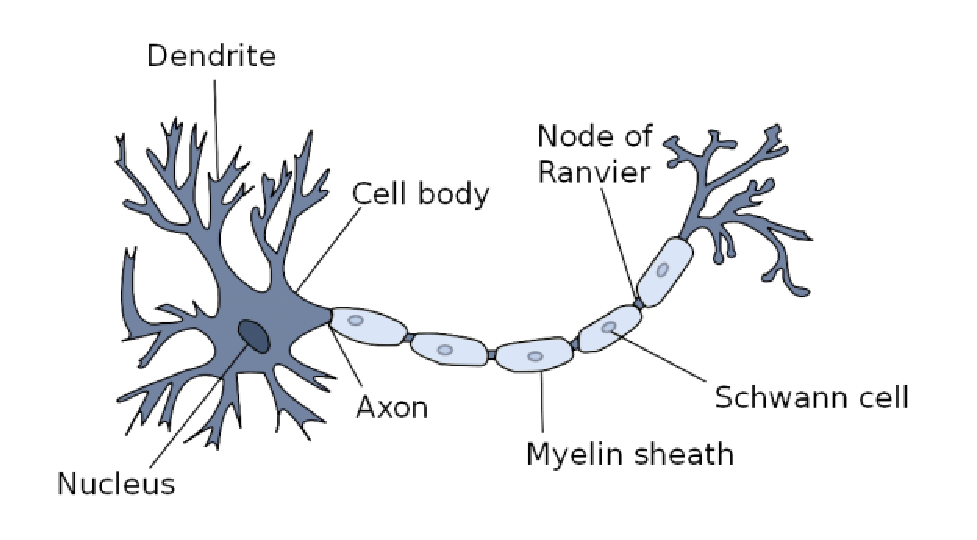
\includegraphics[scale = 0.5]{neuron.eps}
			
			\caption{Simplified representation of a biological neuron, with the components discussed in the text; retrieved from \cite{Kri07}.}
			\label{fig:neuron}
		\end{figure}
		
		The information processing system of a vertebrate can coarsely be divided into the \emph{central nervous system} (CNS) and the \emph{peripheral nervous system} (PNS). The former consists of the \emph{brain} and the \emph{spinal cord}, while the latter mainly comprises the \emph{nerves}, which transmit informations from all other parts of the body to the CNS (\emph{sensory nerves}) and viceversa (\emph{motor nerves}). When an output stimulus hits the sensory cells of an organ sense, these generate an electric signal, called \emph{sensory signal}, which is transfered to the central nervous system via the \emph{sensory nerves}. Within the CNS, informations are stored and managed to provide the muscles with a suitable \emph{motor signal}, broadcast through the \emph{motor nerves} and finally converted by the effectors into a system output \cite{Hay05}.
		
		Hence, both the central and peripheral nervous system are directly involved in the information processing workflow. At the cellular level, this is accomplished through a huge amount of modified cells called \emph{neurons}. These processing elements continuosly communicate with each other by means of electric signals, traveling through a thick net of connections. For instance, in a human being each neuron is linked with $10^3 - 10^4$ other neurons in average. As detailed in the next paragraph, a neuron is characterized by a rather simple structure, specifically designed to rapidly collect input signals and generate an output pulse whenever the accumulated incoming signal exceeds a threshold: the \emph{action potential}. In other terms, a neuron acts as a switch, establishing a typically nonlinear input-output mapping \cite{Kri07}.
		
		From a simplifyed perspective, a neuron consists of three main components: the \emph{dendrites}, the \emph{nucleus} or \emph{soma}, and the \emph{axon}. Dendrites are tree-like networks of nerve fibers receiving input signals from many sources and conveying them directly to the nucleus of the neuron. Here, input signals are accumulated and thresholded, as mentioned before. The possible output pulse is then broadcast to the cells contiguous the neuron through the axon - a unique, slender fiber constituing an extension of the soma and splitting in many branches at the opposite extremity \cite{SD13}. To ease the electrical conduction of the signal, the axon is isolated through a myelin sheath which consists of Schwann cells (in the PNS) or oligodendrocytes (in the CNS). This insulating film is not continuous, rather presents gaps at regular intervals called \emph{nodes of Ranvier}, which allow the signal to be conducted in a saltatory way.
		
		The signal coming from the axon of another neuron or from another cell is transfered to the dendrites of a neuron through a particular connection called \emph{synapsis} \footnote{For the sake of completeness, we mention that there exist synapses directly connecting the axon of the sender neuron with either the soma or the axon of the receiver. Actually, a synapsis may also connect the axon of a neuron with the dendrite or soma of the same neuron (autosynapsis). However, for our purposes we can confine the attention to the axon-dendrite synapsis.}. A synaptic may be either electrical or chemical. In the former, the presynaptic side, i.e., the sender axon, and the postsynapic side, i.e., the receiver dendrite, are directly in contact, so that the potential can simply travel by electrical conduction. Conversely, a chemical synapsis consists of a synaptic \emph{cleft}, physically separating the presynaptic side from the postsynaptic side. Then, to let the action potential reach the postsynaptic side, at the presynaptic side the electrical pulse is converted into a chemical signal. This is accomplished by releasing some chemical substances called \emph{neurotransmitters}. These neurotransmitters then cross the cleft and bind to the receptors dislocated onto the membrane of the postsynaptic side, where the chemical signal is re-converted into an electrical potential. However, neurotransmitters do not simply broadcast the action potential. Indeed, we can distinguish between excitatory and inhibitory neurotransmitters, respectively amplifying or modulating the signal. Hence, the pulse outgoing a neuron is preprocessed within the synapsis before reaching the target cell. In other terms, a neuron receives as input many \emph{weighted} signals, which should then be collected.
		
		 Different studies have unveiled the tight correlation between the synapses which the neurons establish among each other, and the tasks a neural network can address \cite{Hag14}. That is, the set of interneuron connection strengths represent the information storage, i.e., the knowledge, of a neural network \cite{Kri07}. Knowledge is acquired through a \emph{learning} or \emph{training} process, entailing adjustments at the synaptic level to adapt to environmental situations. The adjustments may not only involve the modification of existing synapses, but also the creation of new synaptic connections. Hence, the nervous system is a distributed memory machine whose evolutionary structure is shaped by experience.
		 
		 As mentioned above, a biological neural network acquaints itself with problems of a specific class through a learning procedure. During the learning process, the network is exposed to a collection of situations, giving it the possiblity to derive a set of tools which will let it provide reasonable solutions in similar circumstances. In other terms, the cognitive system should be able to \emph{generalize}. Furthermore, after a successful training, a neural network should show a discrete level of \emph{fault tolerance} against external errors, e.g. noisy inputs. Notice that the nervous system is also naturally fault tolerant against \emph{internal} errors. Indeed, in case a neuron or a (relatively small) group of neurons is damaged or dies, the other processing nodes would take care of its tasks, so that the overall cognitive capabilities would be only slightly affected \cite{Kri07}. 
		 		 
	\vspace*{0.3cm}
		 		
	\section{Artificial neural networks}
	\label{section:Artificial neural networks}
				
		Inspired by the biological information processing system discussed so far, an artificial neural network (ANN), usually simply referred to as "neural network", is a computational model capable to learn from observational data, i.e., by example, thus providing an alternative to the algorithmic programming paradigm \cite{Nie15}. As its original counterpart, it consists of a collection of processing units, called (artificial) neurons, and directed weighted synaptic connections among the neurons. Data travel among neurons through the connections, following the direction imposed by the synapses. Hence, an artificial neural network is an \emph{oriented graph} to all intents and purposes, with the neurons as \emph{nodes} and the synapses as oriented \emph{edges}, whose weights are adjusted by means of a \emph{training} process to configure the network for a specific application \cite{SD13}. 
		
		Formally, a neural network could be defined as follows \cite{Kri07}.
		
		\begin{definition}[Neural network]
			\label{def:neural-network}
			\emph{
			A \emph{neural network} is a sorted triple $\left( \mathcal{N} \, , \mathcal{V} \, , w \right)$, where $\mathcal{N}$ is the set of \emph{neurons}, with cardinality $|\mathcal{N}|$, $\mathcal{V} = \big\lbrace (i \, , j), \, 1 \leq i \, , j  \leq |\mathcal{N}| \big\rbrace$ is the set of \emph{connections}, with $(i,j)$ denoting the oriented connection linking the sending neuron $i$ with the target neuron $j$, and $w : \mathcal{V} \rightarrow \mathbb{R}$ is the \emph{weight function}, defining the weight $w_{i,j} = w((i,j))$ of the connection $(i,j)$. A weight may be either positive or negative, making the underlying connection either excitatory or inhibitory, respectively. By convention, $w_{i,j} = 0$ means that neurons $i$ and $j$ are not directly connected.
			}
		\end{definition}
		
		\noindent In the following, we dive deeper into the structure and training of a neural network, starting by detailing the structure of an artificial neuron.  
		
	\vspace*{0.3cm}
														
	\subsection{Neuronal model}
	\label{section:Neuronal model}
	
		As its name may suggest, an artificial neuron represents a simplified model of a biological neuron, retaining its main features discussed in Section \ref{section:Biological motivation}. To introduce the components of the model, let us consider the neuron $j$ represented in Fig. \ref{fig:neural-model}. Suppose that it is connected with $m$ sending neurons $\big\lbrace s_1, \, \ldots \, , s_m \big\rbrace$, and $n$ receiving (target) neurons $\big\lbrace r_1, \, \ldots \, , r_n \big\rbrace$. Denoting by $y_{\Omega}(t) \in \mathbb{R}$ the scalar output fired by a generic neuron $\Omega$ at time $t$, neuron $j$ gets the weighted inputs $w_{s_k,j} \, y_{s_k}(t)$, $k = 1, \, \ldots \, , m$, at time $t$, and sends out the output $y_j(t + \Delta t)$ to the target neurons $\big\lbrace r_1, \, \ldots \, , r_n \big\rbrace$ at time $t + \Delta t$. In particular, neuron $r_i$, $i = 1, \, \ldots \, , n$, receives as input $w_{j,r_i} \, y_j(t + \Delta t)$. Please note that in the context of artificial neural networks the time is discretized by introducing the timestep $\Delta t$. This is clearly not plausible from a biological viewpoint; however, it substantially simplifies the implementation. In the following, we will avoid to specify the dependence on time unless strictly necessary, thus to lighten the notation.
		
		An artificial neuron $j$ is completely characterized by three functions: the propagation function, the activation function, and the output function. These will be defined and detailed below in the same order they get involved in the data flow. 
		
		\vspace*{0.3cm}
		
		\noindent \textbf{Propagation function}. The propagation function $f_{prop}$ converts the vectorial input \\ $\mathbf{p} = [y_{s_1}, \, \ldots \, , y_{s_m}]^T \in \mathbb{R}^m$ into a scalar $u_{j}$ often called \emph{net input}, i.e.,
		\begin{equation*}
			\label{eq:propagation-function}
			u_{j} = f_{prop}(w_{s_1,j}, \, \ldots \, , w_{s_m,j}, \, y_{s_1}, \, \ldots \, , y_{s_m}) \, .
		\end{equation*}
		A common choice for $f_{prop}$ (used also in this work) is the weighted sum, adding up the scalar inputs multiplied by their respective weights:
		\begin{equation}
			\label{eq:weighted-sum}
			f_{prop}(w_{s_1,j}, \, \ldots \, , w_{s_m,j}, \, y_{s_1}, \, \ldots \, , y_{s_m}) = \sum_{k = 1}^m w_{s_k,j} ~ y_{s_k} \, .
		\end{equation} 
		The function \eqref{eq:weighted-sum} provides a simple, yet effective way of modeling the accumulation of different input electric signals within a biological neuron; this motivates its popularity.
				
		\vspace*{0.3cm}
		
		\noindent \textbf{Activation or transfer function}. At each timestep, the \emph{activation state} $a_j$, often referred to as \emph{activation}, quantifies to which extent neuron $j$ is currently active or excited. It results from the activation function $f_{act}$, which combines the net input $u_j$ with a threshold $\theta_j \in \mathbb{R}$ \cite{Kri07}: 
		\begin{equation*}
			\label{eq:activation-function}
			a_j = f_{act}(u_j; \theta_j) = f_{act} \big( \sum_{k = 1}^m w_{s_k,j} ~ y_{s_k} \, ; \theta_j \big) \, ,
		\end{equation*}
		where we have employed the weighted sum \eqref{eq:weighted-sum} as propagation function. From a biological perspective, the threshold $\theta_j$ is the analogous of the action potential mentioned in Section \ref{section:Biological motivation}. Mathematically, it represents the point where the absolute value of the derivative of the activation function $|f'_{act}|$ is maximum. Then, the activation function reacts particularly sensitive when the net input $u_j$ hits the threshold value $\theta_j$ \cite{Kri07}. \\
		Furthermore, noting that $\theta_j$ is a parameter of the network, one may choose to adapt it through a training process, exactly as it can be done for the synaptic weights, as we shall see in Section \ref{section:Training a multi-layer feedforward neural network}. However, $\theta_j$ is currently included in the activation function, making its runtime access cumbersome. This is typically overcome by introducing a \emph{bias neuron} in the network. A bias neuron is a continuously firing neuron, with constant output $y_{b} = 1$, which gets directly connected with neuron $j$, assigning the \emph{bias weight} $w_{b,j} = - \theta_j$ to the connection. As can be deduced by Fig. \ref{fig:neural-model-bias}, $\theta_j$ is now treated as a synaptic weight, while the neuron threshold is set to zero. Hence, the net input becomes
		\begin{equation}
			\label{eq:net-input}
			u_j = \sum_{k = 1}^m w_{s_k,j} ~ y_{s_k} - \theta_j \, ,
		\end{equation}
		i.e., the threshold is included in the propagation function rather than in the activation function, which we can now express in the form
		\begin{equation*}
			a_j = f_{act} \big( \sum_{k = 1}^m w_{s_k,j} ~ y_{s_k} - \theta_j \big) \, .
		\end{equation*}
		Let us point out that this trick can be clearly applied to all neurons in the network which are characterized by a non-vanishing threshold: it suffices to connect the neuron with the bias, weighting the connection by the opposite of the threshold value. However, for ease of illustration, in the following we avoid to include the bias neuron in any graphical representation of a neural network.
		
		\begin{figure}[t]
			\center
			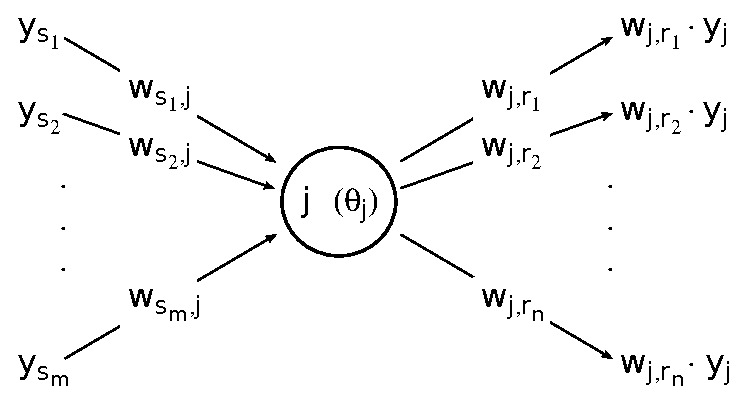
\includegraphics[scale = 0.6]{neural_model_ter.eps}
			
			\caption{Visualization of the generic $j$-th neuron of an artificial neural network. The neuron accumulates the weighted inputs $\big\lbrace w_{s_1,j} ~ y_{s_1}, \, \ldots \, , w_{s_m,j} ~ y_{s_m} \big\rbrace$ coming from the sending neurons $s_1, \, \ldots \, , s_m$, and fires $y_j$, sent to the target neurons $\big\lbrace r_1, \, \ldots \, , r_n \big\rbrace$ through the synapsis $\big\lbrace w_{j,r_1}, \, \ldots \, , w_{j,r_n} \big\rbrace$. The neuron threshold $\theta_j$ is reported within its body.} 
			\label{fig:neural-model}
		\end{figure}
		
		Conversely to the propagation function, there exist various choices for the activation function, e.g., the Heaviside or binary function, which assumes only two values, $0$ or $1$, according to whether the argument is negative or positive, respectively:
		\begin{equation}
			\label{eq:heaviside}
			f_{act}(v) = 
			\begin{cases}
				& 0 \, , \hspace*{0.3cm} \text{if $v < 0$,} \\
				& 1 \, , \hspace*{0.3cm} \text{if $v \geq 0$.}
			\end{cases}
		\end{equation}
		Neurons characterized by such an activation function are usually named McCulloch-Pitts neurons, after the seminal work of McCulloch and Pitts \cite{Hay05}. In addition, note that \eqref{eq:heaviside} is discontinuous, with a vanishing derivative everywhere except in the origin, thus not admissible for the backpropagation training algorithm, as it will explained in Section \ref{section:Training a multi-layer feedforward neural network}. 
		
		Among continuous activation maps, sigmoid functions have been widely used for the realization of artificial neural networks due to their graceful combination of linear and nonlinear behaviour \cite{Hay05}. Sigmoid functions are s-shaped, monotically increasing, and assume values in a bounded interval, typically $[0,1]$, as the logistic function,
		\begin{equation}
			\label{eq:logistic}
			f_{act}(v) = \dfrac{1}{1 + e^{\nicefrac{-v}{T}}} \hspace*{0.3cm} \text{with $T > 0$} \, ,
		\end{equation}
		or $[-1,1]$, as the hyperbolic tangent,
		\begin{equation}
			\label{eq:hyperbolic-tangent}
			f_{act}(v) = \dfrac{e^{v} - e^{-v}}{e^v + e^{-v}} \, .
		\end{equation}
		Both functions are displayed in Fig. \ref{fig:activation-functions}. Note that the logistic function resembles the Heaviside function as $T$ decreases, i.e.,
		\begin{equation*}
			\begin{aligned}
				& \lim_{T \to 0} f_{act}(v) = 0 && \forall v < 0 \, , \\
				& \lim_{T \to 0} f_{act}(v) = 1 && \forall v > 0 \, .
			\end{aligned}
		\end{equation*}
				
		\vspace*{0.3cm}
		
		\noindent \textbf{Output function}. Finally, the output function $f_{out}$ calculates the scalar \emph{output} $y_j \in \mathbb{R}$ based on the activation state $a_j$ of the neuron:
		\begin{equation*}
			\label{eq:output-function}
			y_j = f_{out}(a_j) \, .
		\end{equation*} 
		Typically, $f_{out}$ is the identity function, so that activation and output of a neuron coincides, i.e., $y_j = f_{out}(a_j) = a_j$. Let us point out that, while the input $\mathbf{p} = [y_{s_1}, \, \ldots \, , y_{s_m}]^T \in \mathbb{R}^m$ of the neuron is generally vectorial, i.e., $m > 1$, the output is scalar. The output $y_j$ could then be sent either to other neurons, including the outputting neuron itself (autosynapsis), or constitute a component of the overall output vector of the network, as for the neurons in the output layer of a feedforward neural network (see Section \ref{section:Network topologies}). \\
		It is worth mentioning here that, as the activation function, also the output function is usually \emph{globally} defined, i.e., all neurons in the network (or at least a group of neurons) are equipped with the same output function.
		
		\begin{figure}[t]
			\center
			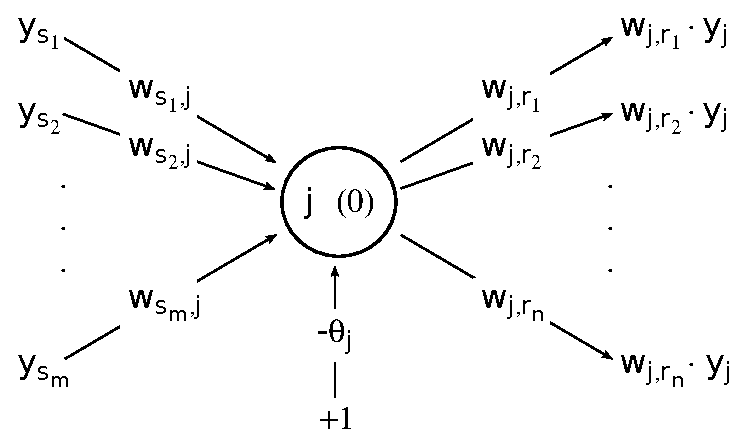
\includegraphics[scale = 0.6]{neural_model_bias.eps}
			
			\caption{Visualization of the generic $j$-th neuron of an artificial neural network. The neuron accumulates the weighted inputs $\big\lbrace w_{s_1,j} ~ y_{s_1}, \, \ldots \, , w_{s_m,j} ~ y_{s_m}, \, -\theta_j \big\rbrace$ coming from the sending neurons $s_1, \, \ldots \, , s_m, \, b$, respectively, with $b$ the bias neuron. The neuron output $y_j$ is then conveyed towards the target neurons $\big\lbrace r_1, \, \ldots \, , r_n \big\rbrace$ through the synapsis $\big\lbrace w_{j,r_1}, \, \ldots \, , w_{j,r_n} \big\rbrace$. Observe that, conversely to the model offered in Fig. \ref{fig:neural-model}, the neuron threshold is now set to $0$.} 
			\label{fig:neural-model-bias}
		\end{figure}
		
		\vspace*{0.3cm}
		
		The neural model presented so far refers to the so called \emph{computing} neuron, i.e., a neuron processing input informations to provide a response. However, in a neural network one may also identify \emph{source} neurons, supplying the network with the respective components of the activation pattern (input vector) \cite{Hay05}. The role of source neurons will become clearer in the next section, where we will introduce the multi-layer feedforward neural network. Here, we just mention that such neuron receives a scalar unweighted input, which is simply forwarded to the connected neurons without performing any computation.
		
	\vspace*{0.3cm}
		
	\subsection{Network topologies: the feedforward neural network}
	\label{section:Network topologies}
			
		The way neurons are interconnected within a network defines the \emph{topology} of the network itself, i.e., its design. In the literature, many network architectures have been proposed, sometimes tailored to a specific application or task. In this section, we expand our investigation for the two most common network topologies: the feedforward and the recurrent neural network.
		
		\begin{figure}[t]
			\center
			\hspace*{-0.4cm}
			\subfloat{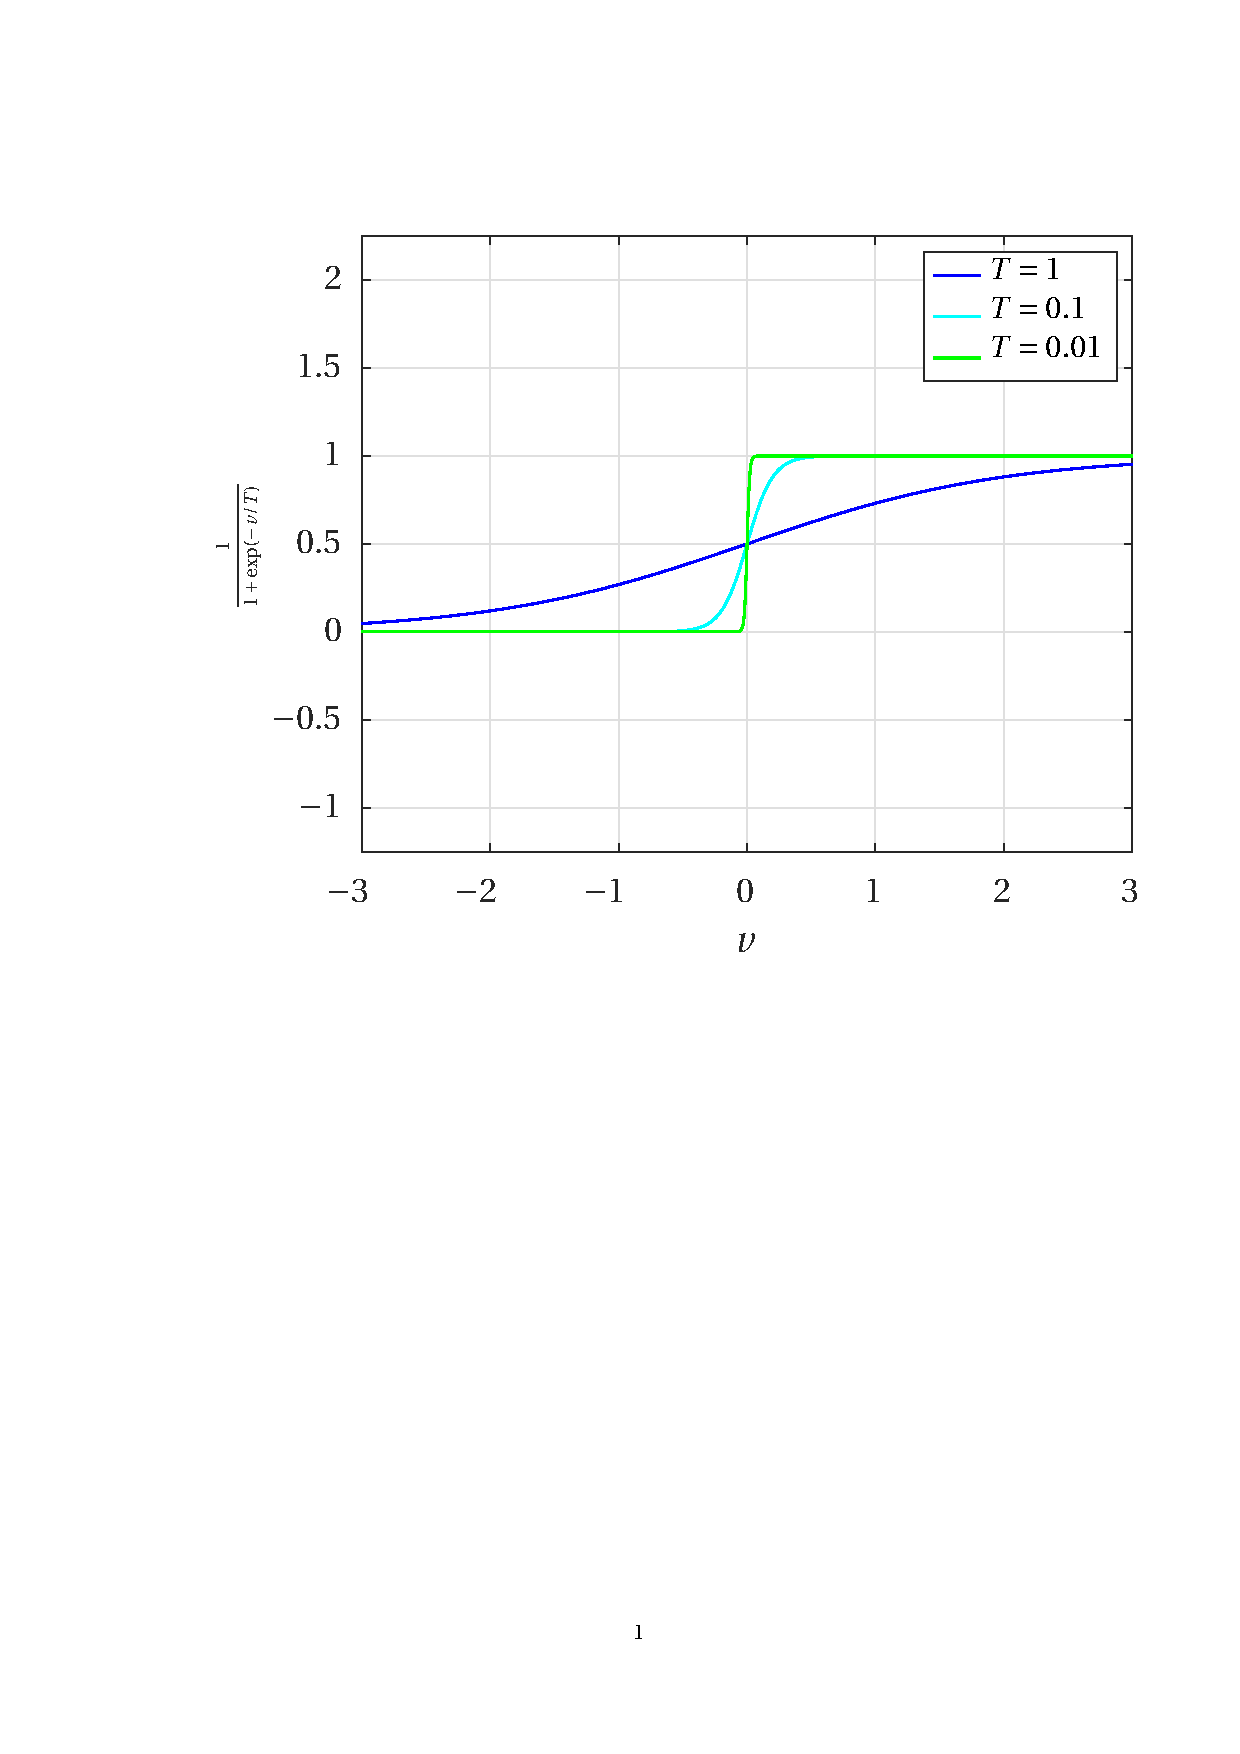
\includegraphics[scale = 0.4, trim = {1cm 11cm 1cm 3.5cm}, clip]{fermi_function_bis}}
			\subfloat{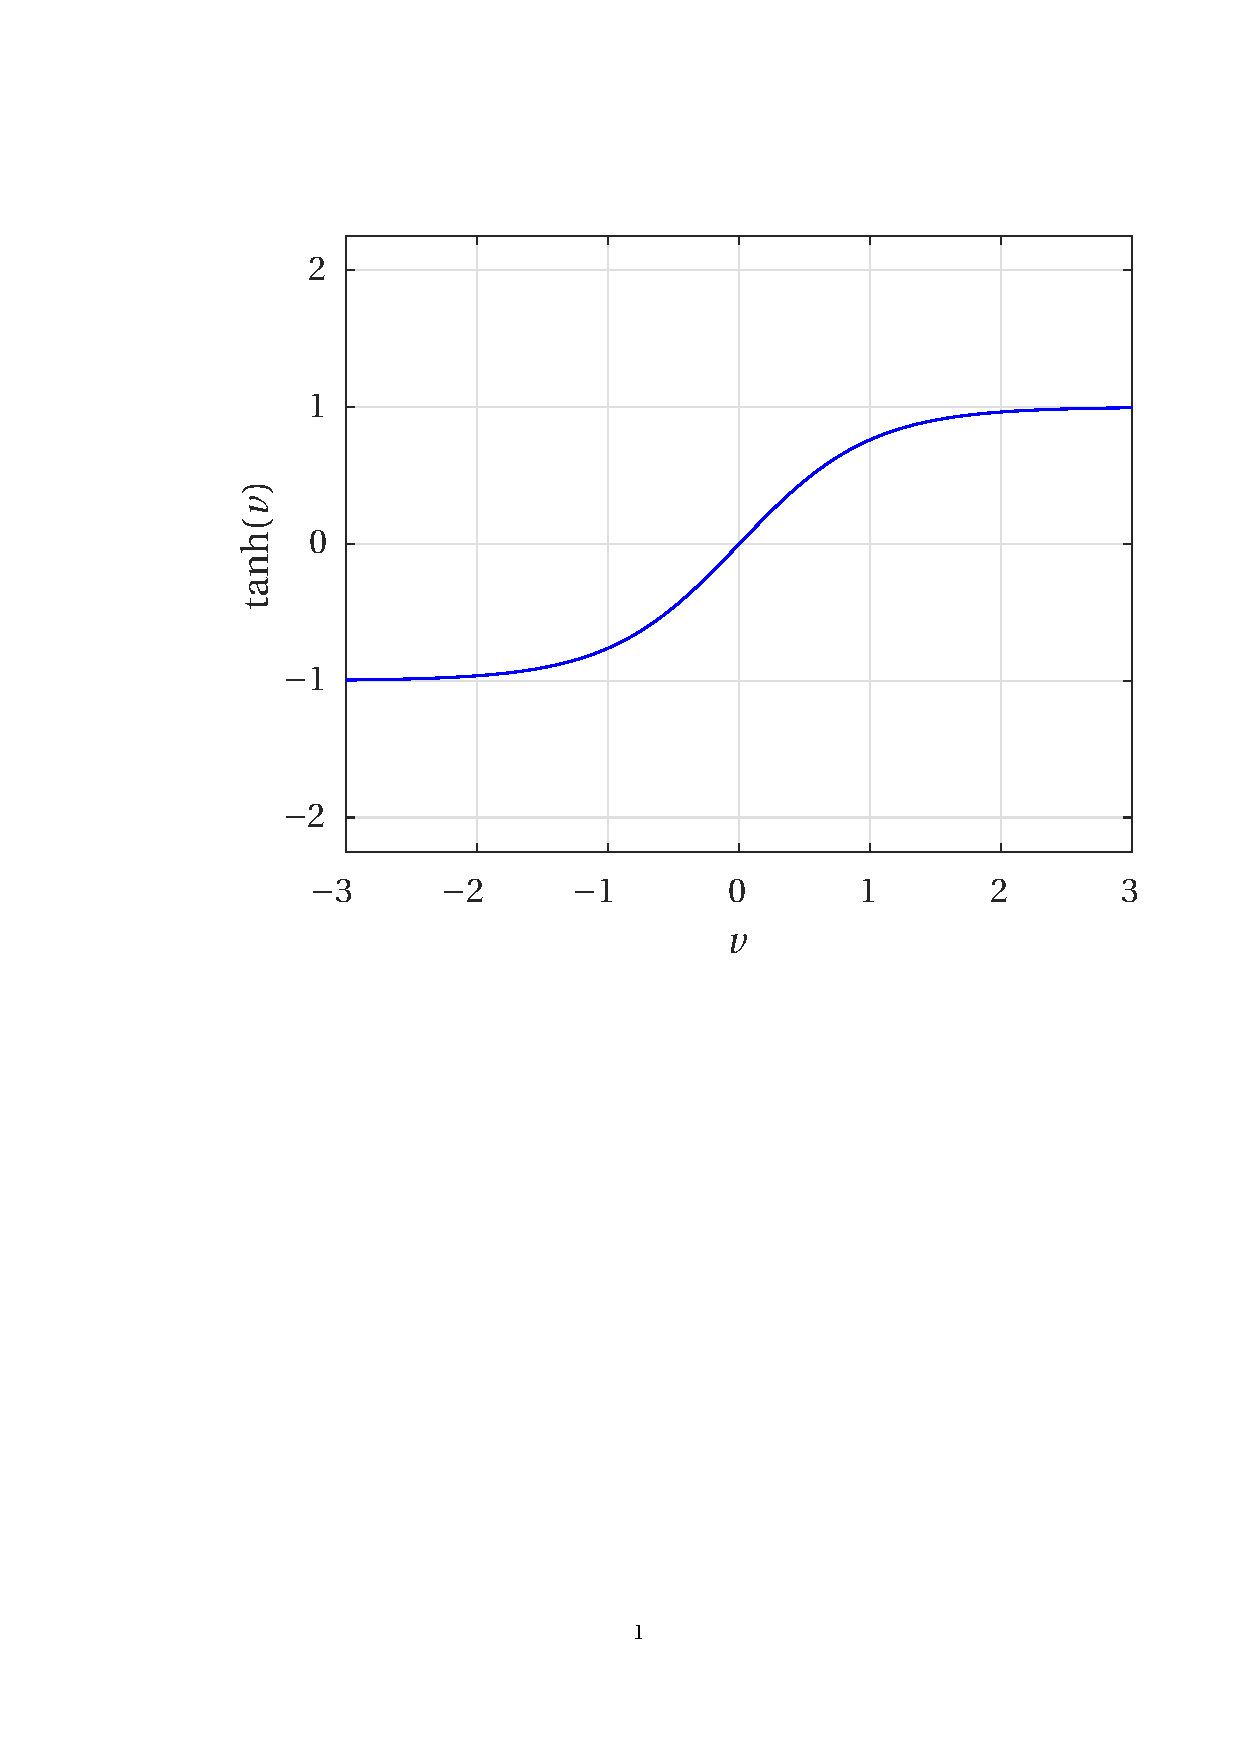
\includegraphics[scale = 0.4, trim = {1cm 11cm 1cm 3.5cm}, clip]{hyperbolic_tangent_bis}}
			
			\caption{Left: logistic function \eqref{eq:logistic} for three values of the parameter $T$; note that as $T$ decreases, the logistic function resembles the Heaviside function. Right: hyperbolic tangent \eqref{eq:hyperbolic-tangent}.}
			\label{fig:activation-functions}
		\end{figure}
		
		\vspace*{0.3cm}
		
		\noindent \textbf{Feedforward neural network}. In a feedforward neural network, also called \emph{perceptron} \cite{Ros58}, neurons are arranged into \emph{layers}, with one \emph{input layer} of $M_I$ source neurons, $K$ \emph{hidden layers}, each one consisting of $H_k$ computing neurons, $k = 1, \, \ldots \, , K$, and an \emph{output layer} of $M_O$ computing neurons. As a characteristic property, neurons in a layer can only be connected with neurons in the next layer towards the output layer, and not within the same layer. Then, an \emph{activation pattern} $\mathbf{p} \in \mathbb{R}^{M_I}$, supplied to the network through the source nodes in the first layer, provides the input signal for the neurons in the first hidden layer. For each hidden layer, its output signals give the input pattern for the following layer. In this way, informations travel towards the last layer of the network, i.e., the output layer, whose outputs constitute the components of the overall output $\mathbf{q} \in \mathbb{R}^{M_O}$ of the network, response to the input pattern $\mathbf{p}$ \footnote{Please note that while the output of a single neuron is denoted with the letter $y$, we use the letter $\mathbf{q}$ (bolded) to indicate the overall output of the network. Clearly, for the $j$-th output neuron the output $y_j$ coincides with the corresponding entry of $\mathbf{q}$, i.e., $q_j = y_j$, $j = 1, \, \ldots \, , M_O$.}. Hence, a feedforward network establishes a map between the \emph{input space} $\mathbb{R}^{M_I}$ and the \emph{output space} $\mathbb{R}^{M_O}$. This makes this network architecture particularly suitable for, e.g., classification and continuous function approximation.
		
		Feedforward networks can be classified according to the number of hidden layers or, equivalently, the number of layers of trainable weights. Single-layer perceptrons (SLPs) consist of the input and output layer, without any hidden layer. Note that the layer which the name SLP refers to is the output layer, while the input layer is not accounted for since no calculations, i.e., information processing operations, occur therein. Because of their quite simple structure, the range of application of SLPs is rather limited. For example, consider a binary input vector and a unique output neuron, with a binary activation function. The SLP network acts then as a classifier, splitting the input space (i.e., the unit hypercube) by means of a hyperplane. Therefore, only \emph{linearly separable} data can be properly represented using SLPs \cite{Kri07}. However, the share of linearly separable sets decreases as the space dimension increases, making SLPs seldom attractive.
		
		Conversely, multi-layer perceptrons (MLPs), with at least one hidden layer, are universal function approximators, as stated by Cybenko \cite{Cyb88, Cyb89}. In detail:
		\begin{enumerate}[label=(\roman*)]
			\item an MLP with one layer of \emph{hidden neurons} and differentiable activation functions can approximate any \emph{continuous} function \cite{Cyb89};
			\label{cybenko-first-rule}
			\item an MLP with two layers of \emph{hidden neurons} and differentiable activation functions can approximate \emph{any function} \cite{Cyb88}.
			\label{cybenko-second-rule}
		\end{enumerate}
		Therefore, in many practical applications there is no reason to employ MLPs with more than two hidden layers. Considering again the binary classifier discussed above, one can represent any convex polygon using one hidden layer and any arbitrary set by using two hidden layers; further increasing the number of hidden neurons would not improve the representation capability of the network. However, \ref{cybenko-first-rule} and \ref{cybenko-second-rule} do not give any practical advice neither on the number of hidden neurons nor the number of samples required to train the network.
		
		An instance of a three-layer (i.e., two hidden layer plus the output layer) feedforward network is offered in Fig. \ref{fig:neural-network}. In this case, we have $M_I = 3$ input neurons (denoted with the letter $i$), $H_1 = H_2 = 6$ hidden neurons (letter $h$ for both hidden layers), and $M_O = 4$ output neurons (letter $o$). In particular, it represents an instance of a \emph{completely linked} perceptron, since each neuron is directly connected with all neurons in the following layer.
		
		Finally, let us just mention that, although we have previously stated that in a feedforward neural network a synapses can only connect pairs of neurons in contiguous layers, recent years have seen the development of different variants. For instance, \emph{shortcut connections} skip one or more layers, while \emph{lateral connections} takes place between neurons within the same layer. However, throughout this work we shall be faithful to the original definition of the perceptron.
				
		\vspace*{0.3cm}
		
		\noindent \textbf{Recurrent neural network}. In recurrent networks any neuron can bind with any other neuron, but autosynapses are forbidden, i.e., the output of a neuron cannot be input into the same neuron at the next time step. If each neuron is connected with all other neurons, then the network is said \emph{completely linked}. As a consequence, one can not distinguish input neurons from output neurons. The input of the network is represented by the initial \emph{network state}, which is the set of activation states for all neurons in the network. Similarly, the overall network output is given by the final network state. Hence, communication between a recurrent neural network and the surrounding environment takes place through the states of the neurons. Examples of recurrent networks are the Hopfield networks \cite{Hop82}, inspired by the behaviour of electrically charged particles within a magnetic field, and the self-organizing maps by Kohonen \cite{Koh98}, highly suitable for cluster detection.
		
		\vspace*{0.3cm}
		
		As mentioned in the introductory chapter, in this work we refer to neural networks for the approximation of the unknown map linking the parameters of a parametrized partial differential equation with the coefficients of the corresponding reduced basis solution. To accomplish this task, we rely on a collection of samples generated through a high-fidelity model. Although a detailed explanation will be provided in Chapter \ref{chapter:Reduced basis methods for nonlinear partial differential equations}, it is worth noticing here that we are interested in a \emph{continuous function approximation} problem. Therefore, a multi-layer feedforward neural network is the most suitable network architecture. 
		
		We will now investigate the way the weights of a perceptron can be \emph{trained}.
		
	\vspace*{0.3cm}
		
	\subsection{Training a multi-layer feedforward neural network}
	\label{section:Training a multi-layer feedforward neural network}
	
		As widely highlighted so far, the principal characteristic of a neural network is its capability of \emph{learning} from the environment by storing the acquired knowledge through the network internal parameters, i.e., the synaptic and bias weights. Learning is accomplished through a training process, during which the network is exposed to a collection of examples, called \emph{training patterns}. According to some performance measure, the weights are then adjusted by means of a well-defined set of rules. Therefore, the learning procedure is an \emph{algorithm}, typically iterative, such that after a successfull training, the neural network provides reasonable responses for unknown problems of the same class of the training set. This property is known as \emph{generalization} \cite{Kri07}. 
		
		Training algorithms can be classified based on the nature of the training set, i.e., the set of training patterns. We can then distinguish three \emph{learning paradigms}.
		
		\vspace*{0.3cm}
		
		\noindent \textbf{Supervised learning}. The training set consists of a collection of \emph{input patterns} (i.e., input vectors) $\big\lbrace \mathbf{p}_i \big\rbrace_{i = 1}^{N_{tr}}$, and corresponding responses $\big\lbrace \mathbf{t}_i \big\rbrace_{i = 1}^{N_{tr}}$, called \emph{teaching inputs}. Then, $\mathbf{t}_i$ is the output the neural network should provide when it receives $\mathbf{p}_i$ as input. As we shall see, any training procedure aims to minimize (in some appropriate norm) the discrepancy between the \emph{desired} output $\mathbf{t}_i$ and the \emph{actual} output $\mathbf{q}_i$ given by the network as response to $\mathbf{p}_i$. 
		
		\vspace*{0.3cm}
		
		\begin{figure}[t]
			\center
			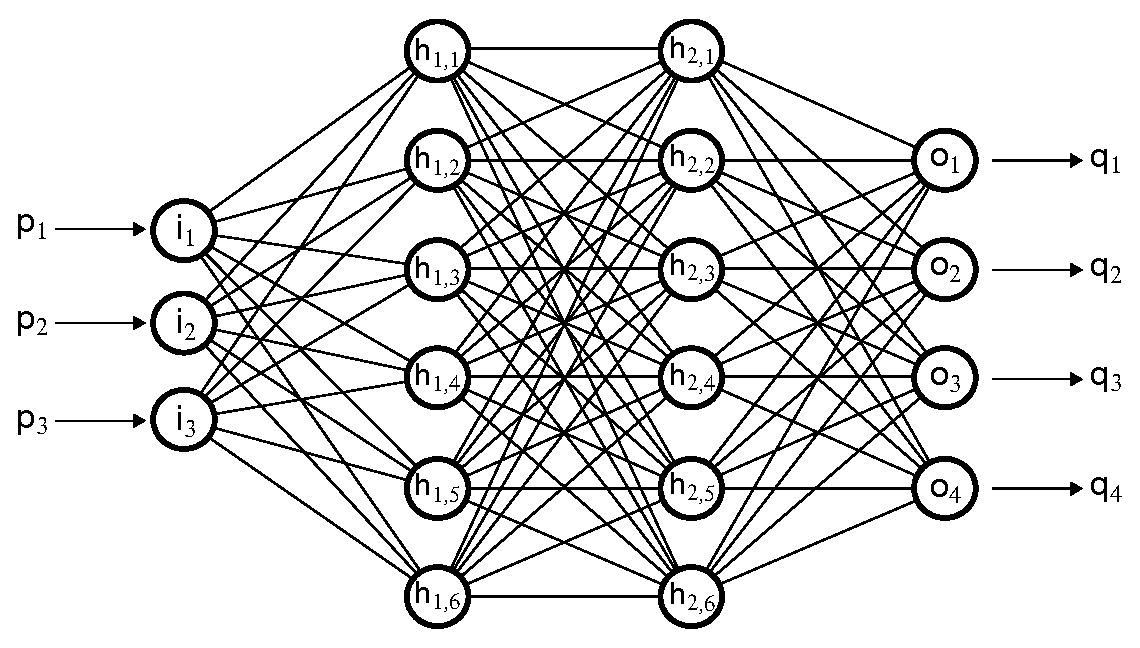
\includegraphics[scale = 0.6]{neural_network_bis.eps}
			
			\caption{A three-layer feedforward neural network, with $3$ input neurons, two hidden layers each one consisting of $6$ neurons, and $4$ output neurons. Within each connection, information flows from left to right.}
			\label{fig:neural-network}
		\end{figure}
		
		\noindent \textbf{Unsupervised learning}. Although supervised learning is a simple and intuitive paradigm, there exist many tasks which require a different approach, as, for instance, a cluster detection problem. Due to lack of prior knowledge, rather than telling the neural network how it should behave in certain situations, one would like the neurons to \emph{independently} identify rules to group items. Therefore, the training pattern is uniquely the input pattern. Since no associated output is provided, such a pattern is referred to as \emph{unlabeled}, as opposed to the \emph{labeled} examples involved in the supervised learning paradigm.
		
		\vspace*{0.3cm}
		
		\noindent \textbf{Reinforcement learning}. Reinforcement learning is the most plausible paradigm from a biological viewpoint. After the completion of a series of input patterns, the neural network is supplied with a boolean or a real number telling whether the behaviour of the network is wrong or right. In the former case, the \emph{feedback} or \emph{reward} may also indicate to which extent the network is wrong \cite{Kri07}. Conversely to the supervised and unsupervised paradigms, reinforcement learning focuses on finding a balance between exploration (of uncharted territory) and exploitation (of current knowledge). Hence, this paradigm particularly suits problems involving a trade-off between a long-term and a short-term reward \cite{KLM96}.
		
		\vspace*{0.3cm}
		
		Clearly, the choice of the learning paradigm is task-dependent. In particular, for function approximation, i.e., what we are interested in, the \emph{supervised learning} paradigm is the best choice. Consider the nonlinear unknown function $\boldsymbol{f}$,
		\begin{equation*}
			\begin{aligned}
				\boldsymbol{f} ~ : ~ & \mathbb{R}^{M_I} \hspace*{-0.3cm} && \rightarrow \mathbb{R}^{M_O} \\
								   & \mathbf{x} && \mapsto \mathbf{y} = \boldsymbol{f}(\mathbf{x}) \, ,
			\end{aligned}
		\end{equation*}
		and a set of labeled examples $\big\lbrace \mathbf{x}_i, \mathbf{y}_i = \bg{f}(\mathbf{x}_i)\big\rbrace_{i = 1}^{N_{tr}}$. The supervised learning paradigm aims at approximating $\boldsymbol{f}$ over a domain $V \subset \mathbb{R}^{M_I}$ up to a user-defined tolerance $\epsilon$, i.e.,
		\begin{equation*}
			||\boldsymbol{F}(\mathbf{x}) - \boldsymbol{f}(\mathbf{x})|| < \epsilon \hspace*{0.3cm} \text{$\forall \mathbf{x} \in V$} \, ,
		\end{equation*}
		where $\mathbf{F} : \mathbb{R}^{M_I} \rightarrow \mathbb{R}^{M_O}$ is the actual input-output map established by the neural network, and $||\cdot||$ is some suitable norm on $\mathbb{R}^{M_O}$. The system should provide accurate predictions for the input patterns, i.e., 
		\begin{equation*}
			\boldsymbol{F}(\mathbf{x}_i) \approx \mathbf{y}_i \, , \hspace*{0.3cm} \text{$\forall i = 1, \, \ldots \, , N_{tr}$} \, .
		\end{equation*} 
		Then, the network is trained through a supervised learning algorithm, employing $\big\lbrace \mathbf{x}_i \big\rbrace_{i = 1}^{N_{tr}}$ as input patterns and $\big\lbrace \mathbf{y}_i \big\rbrace_{i = 1}^{N_{tr}}$ as teaching inputs; that is, 
		\begin{equation*}
			\text{$\mathbf{p}_i = \mathbf{x}_i$ and $\mathbf{t}_i = \mathbf{y}_i$,} \hspace*{0.3cm} \text{$\forall i = 1, \, \ldots \, , N_{tr}$.}
		\end{equation*}
		As defined in the first part of this section, a training algorithm involves:
		\begin{enumerate}[label=(\alph*)]
			\item a set of well-defined rules to modify the synaptic and bias weights;
			\label{a}
			\item a \emph{performance function}, quantifying the current level of knowledge of the surrounding environment.
			\label{b}
		\end{enumerate}
		Regarding \ref{a}, a plethora of weight updating techniques have been proposed in the literature, sometimes tailored to specific applications. Nevertheless, most of them rely on the well-known Hebbian rule, proposed by Donal O. Hebb in 1949 \cite{Heb49}. Inspired by neurobiological considerations, the rule can be stated in a two-steps fashion \cite{Hay05}:
		\begin{enumerate}[label=(\roman*)]
			\item if two neurons on either side of a synapse (connection) are activated simultaneously, then the strength of that synapse is (selectively) increased;
			\label{first-rule}
			\item if two neurons on either side of a synapse are activated asynchronously, then that synapse is selectively weakened (or eliminated).
			\label{second-rule}
		\end{enumerate}
		Actually, \ref{second-rule} was not included in the original statement; nevertheless, it provides a natural extension to \label{first-rule} \cite{Hay05}.
		In mathematical terms, consider the synapsis between a sending neuron $i$ and a target neuron $j$. Then, at the $t$-th iteration (also called \emph{epoch}) of the training procedure, the weight $w_{i,j}(t)$ of the connection $(i,j)$ is modified by the quantity
		\begin{equation}
			\label{eq:hebbian-rule}
			\Delta w_{i,j}(t) \sim \eta ~ y_i(t) ~ a_j(t) \, ,
		\end{equation}
		where $\eta > 0$ is the \emph{learning rate}. We have also exploited the fact that $y_i = a_i$ since the output function is usually represented as the identity. Hence, at the subsequent iteration $t+1$ the synaptic weight is simply given by
		\begin{equation*}
			\label{eq:weight-update}
			w_{i,j}(t+1) = w_{i,j}(t) + \Delta w_{i,j}(t) \, .
		\end{equation*}
		Many of the supervised learning rules proposed in the literature, including the backpropagation of error, can be recast in the following form, which is a generalization of the Hebbian rule \eqref{eq:hebbian-rule} \cite{Kri07}:
		\begin{equation}
			\label{eq:generalized-hebbian-rule}
			\Delta w_{i,j} = \eta ~ h(y_i,w_{i,j}) ~ g(a_j,t_j) \, ,
		\end{equation}
		where $h$ and $g$ depend on the specific learning rule and $t_j$ is the $j$-th component of the teaching input $\mathbf{t}$. Note that all variables involved in \eqref{eq:generalized-hebbian-rule} are supposed to be evaluated at time $t$, i.e., the correction $\Delta w_{i,j}$ is time-dependent. In addition, let us remark that \eqref{eq:generalized-hebbian-rule} represents a \emph{local} and \emph{interactive} mechanism, since it involves both and only the neurons at the end-points of the synapse.
		
		The second ingredient required to define a training algorithm is the performance or error function $E$. This function measures the discrepancy between the neural network knowledge of the surrounding environment and the actual state of the environment itself. In other terms, the bigger the output of the performance function is, the farther the neural network representation of the world is from the actual reality. Therefore, every learning rule aims to \emph{minimize} the performance $E$. For this purpose, $E$ should be a scalar function of the free parameters, i.e., the weights, of the network, namely 
		\begin{equation}
			\label{eq:performance-function}
			E = E(\mathbf{w}) \in \mathbb{R} \, . 
		\end{equation}
		Recalling the notation and assumptions introduced in Definiton \ref{def:neural-network}, here $\mathbf{w} \in \mathbb{R}^{|\mathcal{V}|}$ is a vector collecting the weights $\big\lbrace w_{i,j} = w((i,j)) \big\rbrace_{(i,j) \in \mathcal{V}}$, with $\mathcal{V}$ the set of admissible connections in the network \footnote{Please note that while in Definiton \ref{def:neural-network} $\mathcal{V}$ denoted the set of all \emph{possible} connections, here $\mathcal{V}$ disregards those connections which are not consistent with the network topology in use. For instance, a feedforward neural network can not be endowed with connections oriented towards the input layer. Hence, such connections will not be included in $\mathcal{V}$. In this way, we reduce the size of $\mathbf{w}$ - which is a practical advantage.}. Thus, Eq. \eqref{eq:performance-function} implies that the point over the error surface reached at the end of a successful training process provides the \emph{optimal} configuration $\mathbf{w}_{opt}$ for the network.
		
		The steps for a generic supervised training procedure are listed by Algorithms \ref{alg:online-learning} and \ref{alg:offline-learning} for online and offline learning, respectively. \emph{Online} learning means that the weights are updated after the exposition of the network to each training pattern. In other terms, each epoch involves only one training pattern. Conversely, in an \emph{offline} learning procedure the modifications are based on the entire training set, i.e., the weights are adjusted when the network has received all input patterns and the corresponding errors have been accumulated. Therefore, we should distinguish between the \emph{specific error} $E_{\mathbf{p}}(\mathbf{w})$, specific to the activation pattern $\mathbf{p}$, and the \emph{total error} $E(\mathbf{w})$ that accounts for all specific errors, namely
		\begin{equation}
			\label{eq:accumulated-error}
			E(\mathbf{w}) = \sum_{\mathbf{p} \in P} E_{\mathbf{p}}(\mathbf{w}) \, ,
		\end{equation}
		with $P$ the training set. For instance, we could think of the specific error as the Mean Squared Error (MSE): 
		\begin{equation}
			\label{eq:mse}
			E_{\mathbf{p}}(\mathbf{w}) = \dfrac{1}{M_O} \sum_{j = 1}^{M_O} \left( t_{\mathbf{p},j} - q_{\mathbf{p},j} \right)^2 \, ,
		\end{equation}
		where the subscript $\mathbf{p}$ refers to the input pattern, $\mathbf{t}$ is the teaching input and $\mathbf{q}$ the actual output. Accordingly, the accumulated MSE is:
		\begin{equation}
			\label{eq:accumulated-mse}
			E(\mathbf{w}) = \sum_{\mathbf{p} \in P} E_{\mathbf{p}}(\mathbf{w}) = \sum_{\mathbf{p} \in P} \dfrac{1}{M_O} \sum_{j = 1}^{M_O} \left( t_{\mathbf{p}_i,j} - q_{\mathbf{p}_i,j} \right)^2 \, .
		\end{equation}
				
		\vspace*{0.3cm}
		
		\begin{algorithm}[t]
			\begin{algorithmic}[1]
				\Require neural network $\left( \mathcal{N}, \, \mathcal{V}, \, \mathbf{w}_0 \right)$, training set $P = \big\lbrace \mathbf{p}_i, \, \mathbf{t}_i \big\rbrace_{i = 1}^{N_{tr}}$, 
				\Statex \hspace*{0.535cm} metric $d(\cdot,\cdot) ~ : ~ \mathbb{R}^{M_O} \times \mathbb{R}^{M_O} \rightarrow \mathbb{R}$, tolerance $\epsilon$, maximum number of epochs $T$
				\Ensure trained neural network $\left( \mathcal{N}, \, \mathcal{V}, \, \mathbf{w}_{opt} \right)$
				\vspace*{0.2cm}
				\State $t = 0$, $i = 1$, $k = 0$
				\State $\mathbf{w}(0) = \mathbf{w}_0$
				\While{$t < T$ and $k < N_{tr}$}
					\State evaluate output vector $\mathbf{y}_{\mathbf{p}_i}(t)$, corresponding to input pattern $\mathbf{p}_i$
					\State $E_{\mathbf{p}_i}(\mathbf{w}(t))$ = $d(\mathbf{y}_{\mathbf{p}_i}(t), \, \mathbf{t}_i)$
					\If{$E_{\mathbf{p}_i}(\mathbf{w}(t)) < \epsilon$}
						\State $k \leftarrow k + 1$
					\Else
						\State $k = 0$
						\State compute weight update $\Delta \mathbf{w}(t)$ based on $E_{\mathbf{p}_i}(\mathbf{w}(t))$
						\State $\mathbf{w}(t+1) = \mathbf{w}(t) + \Delta \mathbf{w}(t)$
					\EndIf
					\State $t \leftarrow t+1$, $i \leftarrow i \Mod{N_{tr}} + 1$					
				\EndWhile		
				\State $\mathbf{w}_{opt} = \mathbf{w}(t)$
			\end{algorithmic}
			
			\caption{Online supervised learning algorithm; the procedure ends when all training patterns yield an error below a defined threshold.}
			\label{alg:online-learning}
		\end{algorithm}
		\begin{algorithm}[t]
			\begin{algorithmic}[1]
				\Require neural network $\left( \mathcal{N}, \, \mathcal{V}, \, \mathbf{w}_0 \right)$, training set $P = \big\lbrace \mathbf{p}_i, \, \mathbf{t}_i \big\rbrace_{i = 1}^{N_{tr}}$, 
				\Statex \hspace*{0.535cm} metric $d(\cdot,\cdot) ~ : ~ \mathbb{R}^{M_O} \times \mathbb{R}^{M_O} \rightarrow \mathbb{R}$, tolerance $\epsilon$, maximum number of epochs $T$
				\Ensure trained neural network $\left( \mathcal{N}, \, \mathcal{V}, \, \mathbf{w}_{opt} \right)$
				\vspace*{0.2cm}
				\State $t = 0$
				\State $\mathbf{w}(0) = \mathbf{w}_0$
				\State $E(\mathbf{w}(0))$ = \Call{OfflineError}{$\mathcal{N}$, $\mathcal{V}$, $\mathbf{w}(0)$, $P$, $d$}
				\While{$t < T$ and $E(\mathbf{w}(t)) > \epsilon$}
					\State compute weight update $\Delta \mathbf{w}(t)$ based on $E(\mathbf{w}(t))$
					\State $\mathbf{w}(t+1) = \mathbf{w}(t) + \Delta \mathbf{w}(t)$
					\State $E(\mathbf{w}(t+1))$ = \Call{OfflineError}{$\mathcal{N}$, $\mathcal{V}$, $\mathbf{w}(t+1)$, $P$, $d$}
					\State $t \leftarrow t+1$					
				\EndWhile		
				\State $\mathbf{w}_{opt} = \mathbf{w}(t)$
				\vspace*{0.2cm}
				\Function{$E(\mathbf{w}) = $ OfflineError}{$\mathcal{N}$, $\mathcal{V}$, $\mathbf{w}$, $P$, $d$}
					\State $E(\mathbf{w}) = 0$
					\For{$i = 1, \, \ldots \, , N_{tr}$}
						\State evaluate output vector $\mathbf{y}_{\mathbf{p}_i}$, corresponding to input pattern $\mathbf{p}_i$
						\State $E(\mathbf{w}) \leftarrow E(\mathbf{w}) + d(\mathbf{y}_{\mathbf{p}_i}, \, \mathbf{t}_i)$
					\EndFor
				\EndFunction
			\end{algorithmic}
			
			\caption{Offline supervised learning algorithm; the procedure to compute the accumulated error is also provided.}
			\label{alg:offline-learning}
		\end{algorithm}
		
		\noindent So far, we have not discussed how the update $\Delta w_{i,j}$ for the weight $w_{i,j}$ is practically computed at each iteration. To this end, we have to rigourously define the functions $h$ and $g$ involved in the generalized Hebbian rule \eqref{eq:generalized-hebbian-rule}. Let us recall that any operation of the neural network can be seen as a point over the error surface $E(\mathbf{w})$. Therefore, to increase the performance of the network, we need to iteratively move towards a (local) minimum of the surface \cite{Hay05}. For this purpose, we may employ a \emph{steepest descent} technique, thus following the direction of the anti-gradient, i.e.,
		\begin{equation}
			\label{eq:antigradient}
			\Delta w_{i,j} = - \eta \dfrac{\partial E(\mathbf{w})}{\partial w_{i,j}} \, ,
		\end{equation}
		where $\eta > 0$ is the learning rate that modulates the size of the step. Among the others, the \emph{backpropagation of error} \cite{MR86} is surely the most-known supervised, gradient-based training procedure for a multi-layer feedforward neural network whose neurons are equipped with a \emph{semi-linear}, i.e., continuous and differentiable, activation function \footnote{Therefore, backpropagation cannot be applied with a binary activation function.}. The derivation of the backpropagation algorithm is provided in the following.
		
	\subsubsection{Backpropagation of error}
	\label{section:Backpropagation of error}
		
		Let us consider the generic synapse $(i,j)$ of a multi-layer feedforward neural network, connecting the \emph{predecessor} neuron $i$ with the \emph{successor} neuron $j$. As mentioned before, suppose both $i$ and $j$ present a semi-linear activation function. By exploiting the chain rule, the backpropagation of error provides an operative formula for the evaluation of the antigradient of the error function $E(\mathbf{w})$ in an arbitrary point $\mathbf{w}$, thus allowing to compute the update $\Delta w_{i,j}$ for the weight $w_{i,j}$ according to \eqref{eq:antigradient}. For this purpose, we need to distinguish whether the successor neuron $j$ is either an output or an inner neuron. To improve the clarity of the following mathematical derivation, we add the subscript $\mathbf{p}$ to any variable concerning a neuron.
		
		Let $S = \big\lbrace s_1, \, \ldots \, , s_m \big\rbrace$ be the set of $m$ neurons sending their output to neuron $j$ through the synapses $\big\lbrace (s_1,j), \, \ldots \, , (s_m,j) \big\rbrace$. Recalling the definition \eqref{eq:accumulated-error} of the accumulated error, via the chain rule we can formulate the derivative of $E(\mathbf{w})$ with respect to the weight $w_{i,j}$ as follows:
		\begin{equation}
			\label{eq:bp-first-equation}
			\dfrac{\partial E(\mathbf{w})}{\partial w_{i,j}} = \sum_{\mathbf{p} \in P} \dfrac{\partial E_{\mathbf{p}}(\mathbf{w})}{\partial w_{i,j}} = \sum_{\mathbf{p} \in P} \dfrac{\partial E_{\mathbf{p}}(\mathbf{w})}{\partial u_{\mathbf{p},j}} \dfrac{\partial u_{\mathbf{p},j}}{\partial w_{i,j}} \, .
		\end{equation}
		Assuming the propagation function be represented as the weighted sum, so that the net input is given by \eqref{eq:net-input}, the last factor in \eqref{eq:bp-first-equation} can be written as
		\begin{equation}
			\label{eq:bp-third-equation}
			\dfrac{\partial u_{\mathbf{p},j}}{\partial w_{i,j}} = \dfrac{1}{\partial w_{i,j}} \left( \sum_{s \in S} w_{s,j} ~ y_{\mathbf{p},s} - \theta_j \right) = y_{\mathbf{p},i} \, .
		\end{equation}
		We then denote the opposite of the first term in \eqref{eq:bp-first-equation} by $\delta_{\mathbf{p},j}$, i.e.,
		\begin{equation}
			\label{eq:delta}
			\delta_{\mathbf{p},j} = - \dfrac{\partial E_{\mathbf{p}}(\mathbf{w})}{\partial u_{\mathbf{p},j}} \, .
		\end{equation} 
		$\delta_{\mathbf{p},j}$ is often referred to as the \emph{sensitivity} of the specific error $E_{\mathbf{p}}$ with respect to neuron $j$. Inserting \eqref{eq:delta} and \eqref{eq:bp-third-equation} into \eqref{eq:bp-first-equation} and embedding the resulting equation into \eqref{eq:antigradient}, the weight update can be written as:
		\begin{equation}
			\label{eq:bp-weight-update}
			\Delta w_{i,j} = \eta \sum_{\mathbf{p} \in P} \delta_{\mathbf{p},j} ~ y_{\mathbf{p},i} \, .
		\end{equation}
		We now proceed to derive an operative formula for $\delta_{\mathbf{p},j}$. When $j$ is an output neuron, and using an identity output function, it follows that: 
		\begin{equation}
			\label{eq:bp-fourth-equation}
			\begin{aligned}
				\delta_{\mathbf{p},j} & = - \dfrac{\partial E_{\mathbf{p}}(\mathbf{w})}{\partial y_{\mathbf{p},j}} ~ \dfrac{\partial y_{\mathbf{p},j}}{\partial u_{\mathbf{p},j}} \\
				& = - \dfrac{1}{\partial y_{\mathbf{p},j}} \dfrac{1}{M_O} \sum_{k = 1}^{M_O} \left( t_{\mathbf{p},k} - y_{\mathbf{p},k} \right)^2 ~ \dfrac{\partial a_{\mathbf{p},j}}{\partial u_{\mathbf{p},j}} \\
				& = \dfrac{2}{M_O} \left( t_{\mathbf{p},j} - y_{\mathbf{p},j} \right) ~ \dfrac{\partial f_{act}(u_{\mathbf{p},j})}{\partial u_{\mathbf{p},j}} \\
				& = \dfrac{2}{M_O} \left( t_{\mathbf{p},j} - y_{\mathbf{p},j} \right) ~ f'_{act}(u_{\mathbf{p},j}) \, ,
			\end{aligned}
		\end{equation}
		where we have used the specific error given in \eqref{eq:mse}. As appears in \eqref{eq:bp-fourth-equation}, we must require a differentiable transfer function.
				
		It is worth mentioning that \eqref{eq:bp-fourth-equation} does not apply when $j$ lies within a hidden layer as no teaching input is provided for a hidden neuron. In that case, we denote by $R = \big\lbrace r_1, \, \ldots \, , r_n \big\rbrace$ the set of $n$ neurons receveing the output generated by $j$, called the \emph{successors}. We then note that the output of any neuron can directly affect only its successors \cite{Kri07}. Hence: 
		\begin{equation}
			\label{eq:bp-fifth-equation}
			\begin{aligned}
				\delta_{\mathbf{p},j} & = \dfrac{\partial E_{\mathbf{p}}(\mathbf{w})}{\partial u_{\mathbf{p},j}} \\
				& = \dfrac{\partial E_{\mathbf{p}}(u_{\mathbf{p},r_1}, \, \ldots \, , u_{\mathbf{p},r_n})}{\partial u_{\mathbf{p},j}} \\
				& = \dfrac{\partial E_{\mathbf{p}}(u_{\mathbf{p},r_1}, \, \ldots \, , u_{\mathbf{p},r_n})}{\partial y_{\mathbf{p},j}} ~ \dfrac{\partial y_{\mathbf{p},j}}{\partial u_{\mathbf{p},j}} \\
				& = \sum_{k = 1}^{n} \dfrac{\partial E_{\mathbf{p}}}{\partial u_{\mathbf{p},r_k}} ~ \dfrac{\partial u_{\mathbf{p},r_k}}{\partial y_{\mathbf{p},j}} ~ \dfrac{\partial y_{\mathbf{p},j}}{\partial u_{\mathbf{p},j}} \, .
			\end{aligned}
		\end{equation}
		Applying the definition of sensitivity for neuron $r_k$, $k = 1, \, \ldots \, , n$, under the same assumptions of Eq. \eqref{eq:bp-fourth-equation} we can further develop \eqref{eq:bp-fifth-equation}:
		\begin{equation}
			\label{eq:bp-sixth-equation}
			\begin{aligned}
			\delta_{\mathbf{p},j} & = \sum_{k = 1}^n \left( - \delta_{\mathbf{p},r_k} \right) ~ \dfrac{1}{\partial y_{\mathbf{p},j}} \left( \sum_{l = 1}^{m_k} w_{s_l,r_k} y_{\mathbf{p},s_l} - \theta_{r_k} \right) ~ \dfrac{\partial f_{act}(u_{\mathbf{p},j})}{\partial u_{\mathbf{p},j}} \\
			& = - \sum_{k = 1}^n \delta_{\mathbf{p},r_k} ~ w_{j,r_k} ~ f'_{act}(u_{\mathbf{p},j}) \, .
			\end{aligned}
		\end{equation}
		Here, we have supposed that $r_k$ receives input signals from $m_k$ neurons $\big\lbrace s_1, \, \ldots \, s_{m_k} \big\rbrace$.
		
		Let us now summarize the results derived so far. At any iteration $t$ of the backpropagation learning algorithm, the weight $w_{i,j}(t)$ of a generic connection $(i,j)$ linking neuron $i$ with neuron $j$ is corrected by an additive quantity $\Delta w_{i,j}(t)$, i.e., 
		\begin{equation*}
			w_{i,j}(t+1) = w_{i,j}(t) + \Delta w_{i,j}(t) \, .
		\end{equation*}
		By using the accumulated MSE \eqref{eq:accumulated-mse} as performance function and understanding the dependence on time for the sake of clarity, the weight update $\Delta w_{i,j}$ reads:
		\begin{equation*}
			\Delta w_{i,j} = \eta \sum_{\mathbf{p} \in P} y_{\mathbf{p},i} ~ \delta_{\mathbf{p},j} \, ,
		\end{equation*}
		where $\eta > 0$ and $\delta_{\mathbf{p},j}$ is given by
		\begin{subnumcases}{\delta_{\mathbf{p},j} =}
			\label{eq:bp-inner-neuron}
		   	f'_{act}(u_{\mathbf{p},j}) \sum_{r \in R} \delta_{\mathbf{p},r} ~ w_{j,r} \, , & \text{if $j$ inner neuron} \, , \\
		   	\label{eq:bp-output-neuron}
			\dfrac{2}{M_O} f'_{act}(u_{\mathbf{p},j}) \left( t_{\mathbf{p},j} - y_{\mathbf{p},j} \right) \, , & \text{if $j$ output neuron} \, .
		\end{subnumcases}
		Some relevant remarks about the overall algorithm should be made. First, observe that \eqref{eq:bp-inner-neuron} defines $\delta_{\mathbf{p},j}$ for a hidden node $j$ by relying on the neurons in the following layer, whereas \eqref{eq:bp-output-neuron} only involves variables concerning the neuron itself (namely, $u_{\mathbf{p},j}$ and $y_{\mathbf{p},j}$) and the exact output $t_{\mathbf{p},j}$. Therefore, the coupled equations \eqref{eq:bp-inner-neuron}-\eqref{eq:bp-output-neuron} implicitly set the order in which the weights must be adjusted: starting from the output layer, update all the connections ending in that layer, then move backwards to the preceeding layer. In this way, the error is \emph{backpropagated} from the output down to the input, leaving traces in each layer of the network \cite{Kri07, WH60}.
		
		The weight updating procedure detailed above corresponds to the offline version of the backpropagation of error, since it involves the total error $E$. However, the online algorithm readly comes from \eqref{eq:bp-weight-update} by simply dropping the summation over the elements of the training set $P$.
		
		Although intuitive and very promising, backpropagation of error suffers from all drawbacks that are peculiar to gradient-based techniques. For instance, we may get stuck in a local minimum, whose level is possibly far from the global minimum of the error surface $E$. Furthermore, since the step size dictated by the gradient method is given by the norm of the gradient itself, minima close to steepest gradients are likely to be missed due to a large step size. This motivates the introduction in \eqref{eq:antigradient} of the learning rate $\eta \in (0,1]$, which acts as a reducing factor and thus enables a better control on the descent. As suggested by Kriesel \cite{Kri07}, in many applications reasonable values for $\eta$ lies in the range $[0.01,0.9]$. In particular, a time-dependent learning rate usually enables a more effective and more efficient training procedure. On the one hand, at the beginning of the process, when the network is far from the application goal, one often needs to span a large extent of the error landscape, to identify a region of interest. At that time, the learning rate should be large, i.e., close to $1$, to speed up the exploration. On the other hand, as we approach the optimal configuration, we may want to progressively reduce the learning rate, thus the step size, to fine-tune the weights of the neural network. 
		
		Nevertheless, selecting an appropriate value for $\eta$ remains more an art than a science. Furthermore, the derivative of sigmoidal activations functions (see Fig. \ref{fig:activation-functions}) is close to zero far from the origin. As a consequence, it becomes very difficult to move neurons away from the limits of the activation, which could extremely extend the learning time \cite{Kri07}. Hence, different alternatives to backpropagation have been proposed in the literature, either by modifying the original algorithm (as, e.g., the resilient backpropagation \cite{RB93} or the quickpropagation \cite{Fah88}), or pursuing a different numerical approach to the optimization problem. The latter class of algorithms includes the Levenberg-Marquardt algorithm, which we use extensively in our numerical tests.
				
		\subsubsection{Levenberg-Marquardt algorithm}
		\label{section:Levenberg-Marquardt algorithm}
		
		While backpropagation is a steepest descent algorithm, the Levenberg-Marquardt algorithm \cite{Mar63} is an approximation to Newton's method \cite{Hag94}. As for backpropagation, the learning procedure is driven by the loss function $E = E(\mathbf{w})$, $\mathbf{w} \in \mathbb{R}^{|\mathcal{V}|}$. Applying Newton's method for the minimization of $E$, at each iteration the \emph{search direction} $\Delta \mathbf{w}$ is found by solving the following linear system:
		\begin{equation}
			\label{eq:newton}
			\nabla^2 E(\mathbf{w}) \Delta \mathbf{w} = - \nabla E(\mathbf{w}) \, ,
		\end{equation}
		where $\nabla E(\mathbf{w})$ and $\nabla^2 E(\mathbf{w})$ denotes, respectively, the gradient vector and the Hessian matrix of $E$ with respect to its argument $\mathbf{w}$. Assume now that the loss function is represented as the accumulated MSE, 
		\begin{equation*}
			\label{eq:accumulated-mse-bis}
			E(\mathbf{w}) = \sum_{\mathbf{p} \in P} \dfrac{1}{M_O} \sum_{j = 1}^{M_O} \left( t_{\mathbf{p},j} - y_{\mathbf{p},j} \right)^2 = \sum_{\mathbf{p} \in P} \dfrac{1}{M_O} \sum_{j = 1}^{M_O} e_{\mathbf{p},j}(\mathbf{w})^2 \, ;
		\end{equation*}
		with $e_{\mathbf{p},j}$ the $j$-th component of the error vector $\mathbf{e}_{\mathbf{p}} = \mathbf{t}_{\mathbf{p}} - \mathbf{y}_{\mathbf{p}}$ corresponding to the input pattern $\mathbf{p}$. Then, introducing the Jacobian $J_{\mathbf{p}}$ of the specific error vector $\mathbf{e}_{\mathbf{p}}$ with respect to $\mathbf{w}$, i.e., 
		\begin{equation}
			\label{eq:jacobian}
			J_{\mathbf{p}}(\mathbf{w}) = 
			\begin{bmatrix}
				\vspace*{0.2cm}
				\hspace*{-0.3cm} & \dfrac{\partial e_{\mathbf{p},1}}{\partial w_1} & \dfrac{\partial e_{\mathbf{p},1}}{\partial w_2} & \ldots & \dfrac{\partial e_{\mathbf{p},1}}{\partial w_{|\mathcal{V}|}} \\
				\vspace*{0.2cm}
				\hspace*{-0.3cm} & \dfrac{\partial e_{\mathbf{p},2}}{\partial w_1} & \dfrac{\partial e_{\mathbf{p},2}}{\partial w_2} & \ldots & \dfrac{\partial e_{\mathbf{p},2}}{\partial w_{|\mathcal{V}|}} \\
				\vspace*{0.2cm}
				\hspace*{-0.3cm} & \vdots & \vdots & \ddots & \vdots \\
				\hspace*{-0.3cm} & \dfrac{\partial e_{\mathbf{p},M_O}}{\partial w_1} & \dfrac{\partial e_{\mathbf{p},M_O}}{\partial w_2} & \ldots & \dfrac{\partial e_{\mathbf{p},M_O}}{\partial w_{|\mathcal{V}|}}
			\end{bmatrix}
			\in \mathbb{R}^{M_O \times |\mathcal{V}|}
		\end{equation}
		simple computations yield:
		\begin{equation}
			\label{eq:gradient}
			\nabla E(\mathbf{w}) = \sum_{\mathbf{p} \in P} \dfrac{2}{M_0} J_{\mathbf{p}}(\mathbf{w})^T \mathbf{e}_{\mathbf{p}} \in \mathbb{R}^{|\mathcal{V}|}
		\end{equation}
		and
		\begin{equation}
			\label{eq:hessian}
			\nabla^2 E(\mathbf{w}) = \sum_{\mathbf{p} \in P} \dfrac{2}{M_O} \left[ J_{\mathbf{p}}(\mathbf{w})^T J_{\mathbf{p}}(\mathbf{w}) + S(\mathbf{w}) \right] \in \mathbb{R}^{|\mathcal{V}| \times |\mathcal{V}|} \, ,
		\end{equation}
		with
		\begin{equation*}
			S(\mathbf{w}) = \sum_{\mathbf{p} \in P} \dfrac{2}{M_O} \sum_{j = 1}^{M_O} e_{\mathbf{p},j} \nabla^2 e_{\mathbf{p},j} \, .
		\end{equation*}
		Assuming $S(\mathbf{w}) \approx 0$, inserting \eqref{eq:gradient} and \eqref{eq:hessian} into \eqref{eq:newton} we get the linear system
		\begin{equation}
			\label{eq:newton-quadratic-function}
			\left[ \sum_{\mathbf{p} \in P} J_{\mathbf{p}}(\mathbf{w})^T J_{\mathbf{p}}(\mathbf{w}) \right] \Delta \mathbf{w} = - \sum_{\mathbf{p} \in P} J_{\mathbf{p}}(\mathbf{w})^T \mathbf{e}_{\mathbf{p}}(\mathbf{w}) \, .
		\end{equation} 
		The Levenberg-Marquardt modification to Newton's method reads \cite{Hag94, Mar63}:
		\begin{equation}
			\label{eq:levenberg-marquardt}
			\left[ \sum_{\mathbf{p} \in P} J_{\mathbf{p}}(\mathbf{w})^T J_{\mathbf{p}}(\mathbf{w}) + \mu I \right] \Delta \mathbf{w} = - \sum_{\mathbf{p} \in P} J_{\mathbf{p}}(\mathbf{w})^T \mathbf{e}_{\mathbf{p}}(\mathbf{w}) \, ,
		\end{equation}
		with $\mu \geq 0$ and $I$ the identity matrix of size $|\mathcal{V}| \times |\mathcal{V}|$. Note that if $\mu = 0$ we recover Newton's method \eqref{eq:newton-quadratic-function}, while for $\mu \gg 1$ the search direction $\Delta \mathbf{w}$ approaches antigradient of $E$, i.e., we recover the backpropagation algorithm. Then, the Levenberg-Marquardt algorithm can be seen as an interpolation between Newton's method and the steepest descent method, aiming to retain the advantages of both techniques.
		
		The Levenberg-Marquardt training algorithm proceeds as follows. At each epoch $t$ of the training procedure, we solve the (potentially large) linear system \eqref{eq:levenberg-marquardt}. Whenever the step $\Delta \mathbf{w}(t)$ leads to a reduction in the performance function, i.e., $E(\mathbf{w}(t) + \Delta \mathbf{w}(t)) < E(\mathbf{w}(t))$, the parameter $\mu$ is reduced by a factor $\beta > 1$. Conversely, if $E(\mathbf{w}(t) + \Delta \mathbf{w}(t)) > E(\mathbf{w}(t))$ the parameter is multiplied by the same factor $\beta$. This reflects the idea that far from the actual minimum we should prefer the gradient method to Newton's method, since the latter may diverge. Yet, once in a neighborhood of the minimum, we switch to Newton's method so to exploit its faster convergence \cite{Mar63}.
		
		The key step in the algorithm is the computation of the Jacobian $J_{\mathbf{p}}(\mathbf{w})$ for each training vector $\mathbf{p}$. Suppose that the $k$-th element $w_k$ of $\mathbf{w}$ represents the weight $w_{i,j}$ of the connection $(i,j)$, for some $i$ and $j$, with $1 \leq i \, , j \leq |\mathcal{N}|$, i.e., $w_k = w_{i,j}$. Since
		\begin{equation*}
			\dfrac{\partial e_{\mathbf{p},h}}{\partial w_{i,j}}
		\end{equation*}
		is related with the gradient of the performance function, we can follow the same steps performed to derive the backpropagation, namely:
		\begin{equation}
			\label{eq:jacobian-entry-equation}
			\begin{aligned}
				\dfrac{\partial e_{\mathbf{p},h}}{\partial w_{i,j}} & = \dfrac{\partial e_{\mathbf{p},h}}{\partial u_{\mathbf{p},j}} ~ \dfrac{\partial u_{\mathbf{p},j}}{\partial w_{i,j}} \\[0.1cm]
				& = \dfrac{\partial e_{\mathbf{p},h}}{\partial y_{\mathbf{p},j}} ~ \dfrac{\partial y_{\mathbf{p},j}}{\partial u_{\mathbf{p},j}} ~ \dfrac{\partial u_{\mathbf{p},j}}{\partial w_{i,j}} \\[0.1cm]
				& = \dfrac{\partial e_{\mathbf{p},h}}{\partial y_{\mathbf{p},j}} ~ f'_{act}(u_{\mathbf{p},j}) ~ y_{\mathbf{p},i} \\
				& = \delta_{\mathbf{p},h,j} ~ y_{\mathbf{p},i} \, ,
			\end{aligned}
		\end{equation} 
		with
		\begin{equation}
			\label{eq:levenberg-marquardt-delta}
			\delta_{\mathbf{p},h,j} := - \dfrac{\partial e_{\mathbf{p},h}}{\partial u_{\mathbf{p},j}} = - \dfrac{\partial e_{\mathbf{p},h}}{\partial y_{\mathbf{p},j}} ~ f'_{act}(u_{\mathbf{p},j}) \, .
		\end{equation}
		For the computation of the derivative 
		\begin{equation*}
			\dfrac{\partial e_{\mathbf{p},h}}{\partial y_{\mathbf{p},j}}
		\end{equation*}
		occurring in \eqref{eq:levenberg-marquardt-delta}, we assume that, within the set of neurons $\mathcal{N}$, items are ordered such that the output neurons come first, i.e.,
		\begin{equation*}
			\text{$j$ output neuron \hspace*{0.2cm} $\Leftrightarrow$ \hspace*{0.2cm} $1 \leq j \leq M_O$} \, .
		\end{equation*} 
		We can then distinguish three cases:
		\begin{enumerate}[label=(\roman*)]
			\item $j$ output neuron, $j = h$: since $e_{\mathbf{p},h} = e_{\mathbf{p},j} = t_{\mathbf{p},j} - y_{\mathbf{p},j}$, then 
			\begin{equation*}
				\label{eq:jacobian-first-case}
				\dfrac{\partial e_{\mathbf{p},h}}{\partial y_{\mathbf{p},j}} = -1 \, ;
			\end{equation*}
			\item $j$ output neuron, $j \neq h$: the output of an output neuron can not influence the signal fired by another output neuron, hence 
			\begin{equation*}
				\label{eq:jacobian-second-case}
				\dfrac{\partial e_{\mathbf{p},h}}{\partial y_{\mathbf{p},j}} = 0 \, ;
			\end{equation*}
			\item $j$ inner neuron: letting $R$ be the set of successors of $j$, similarly to \eqref{eq:bp-sixth-equation} the chain rule yields
			\begin{equation*}
				\label{eq:jacobian-third-case}
				\dfrac{\partial e_{\mathbf{p},h}}{\partial y_{\mathbf{p},j}} = \sum_{r \in R} \dfrac{\partial e_{\mathbf{p},h}}{\partial u_{\mathbf{p},r}} ~ \dfrac{\partial u_{\mathbf{p},r}}{\partial y_{\mathbf{p},j}} = - \sum_{r \in R} \delta_{\mathbf{p},h,r} ~ w_{j,r} \, .
			\end{equation*}
		\end{enumerate}
		Ultimately, at any iteration of the learning algorithm, the entries of the Jacobian matrix $J_{\mathbf{p}}$ are given by
		\begin{equation*}
			\dfrac{\partial e_{\mathbf{p},h}}{\partial w_k} = \delta_{\mathbf{p},h,j} ~ y_{\mathbf{p},i} \, , \hspace*{0.3cm} 1 \leq h \leq M_O \, , 1 \leq k \leq |\mathcal{V}| \, , \text{$w_k = w_{i,j}$ for some $i$ and $j$} \, ,
		\end{equation*}
		with
		\begin{subnumcases}{\delta_{\mathbf{p},h,j} =}
			\label{eq:levenberg-marquardt-inner-neuron}
		   	f'_{act}(u_{\mathbf{p},j}) \sum_{r \in R} \delta_{\mathbf{p},h,r} ~ w_{j,r} \, , & \text{if $j$ inner neuron} \, , \\
		   	\label{eq:levenberg-marquardt-output-neuron}
			f'_{act}(u_{\mathbf{p},j}) \delta_{jh}^K \, , & \text{if $j$ output neuron} \, ,
		\end{subnumcases}
		where $\delta_{jh}^K$ is the Kronecker delta. The steps to be performed at each iteration of the Levenberg-Marquardt algorithm are summarized in Algorithm \ref{alg:levenberg-marquardt}.
		
		Let us finally remark that a trial and error approach is still required to find satisfactory values for $\mu$ and $\beta$; as proposed in \cite{Mar63}, a good starting point may be $\mu = 0.01$, with $\beta = 10$. Moreover, the dimension of the system \eqref{eq:levenberg-marquardt} increases nonlinearly with the number of neurons in the network, making the Levenberg-Marquardt algorithm poorly efficient for large networks \cite{Hag94}. However, it is more efficient than backpropagation for networks with a few hundreads of connections, besides producing much more accurate results. We will further develop this topic in Chapter \ref{chapter:Numerical results}.
		
		\begin{algorithm}[H]
			\begin{algorithmic}[1]
				\Function{$\left[ \mathbf{w} + \Delta \mathbf{w}, \, E(\mathbf{w} + \Delta \mathbf{w}), \, \mu \right]$ = LMiteration}{$\mathcal{N}$, $\mathcal{V}$, $\mathbf{w}$, $P$, $E(\mathbf{w})$, $d$, $\mu$}
					\State $\beta = 10$
					\For{$i = 1, \, \ldots \, , N_{tr}$}
						\State evaluate output vector $\mathbf{y}_{\mathbf{p}_i}$, corresponding to input pattern $\mathbf{p}_i$
						\State $\mathbf{e}_{\mathbf{p}_i} = \mathbf{y}_{\mathbf{p}_i} - \mathbf{t}_{\mathbf{p}_i}$
						\For{$h = 1, \, \ldots \, , M_0$, $k = 1, \, \dots \, , |\mathcal{V}|$}
							\State compute $\left( J_{\mathbf{p}_i} \right)_{h,k}$ according to \eqref{eq:jacobian-entry-equation}, \eqref{eq:levenberg-marquardt-inner-neuron} and \eqref{eq:levenberg-marquardt-output-neuron} 
						\EndFor
					\EndFor
					\State assemble and solve $\left[ \sum_{i = 1}^{N_{tr}} J_{\mathbf{p}_i}^T J_{\mathbf{p}_i} + \mu I \right] \Delta \mathbf{w} = - \sum_{i = 1}^{N_{tr}} J_{\mathbf{p}_i}^T \mathbf{e}_{\mathbf{p}_i}$
					\State $E(\mathbf{w} + \Delta \mathbf{w})$ = \Call{OfflineError}{$\mathcal{N}$, $\mathcal{V}$, $\mathbf{w} + \Delta \mathbf{w}$, $P_{tr}$, $d$}
					\If{$E(\mathbf{w} + \Delta \mathbf{w}) < E(\mathbf{w})$}
						\State $\mu \leftarrow \mu / \beta$
					\Else
						\State $\mu \leftarrow \mu * \beta$
					\EndIf 
				\EndFunction
			\end{algorithmic}
			
			\caption{An iteration of the Levenberg-Marquardt training algorithm.}
			\label{alg:levenberg-marquardt}
		\end{algorithm}
						
	\subsection{Practical considerations on the design of artificial neural networks}
	\label{section:Practical considerations on the design of artificial neural networks}
	
		We conclude this introductory chapter on neural networks by discussing the major concerns regarding their design and implementation, mainly focusing on MLPs. As we shall see, most of these issues are still open questions in many research fields, and as such they should be tackled pursuing a \emph{trial-and-error} approach.
		
		In Section \ref{section:Network topologies}, we reported two fundamental results (\ref{cybenko-first-rule} and \ref{cybenko-second-rule}) promoting three-layers feedforward neural networks as universal function approximators. Yet, these statements do not provide any information regarding the number of neurons and training patterns required to approximate a function up to a desired level of uncertainty. In other terms, \ref{cybenko-first-rule} and \ref{cybenko-second-rule} are not operative, and therefore one has to rely on emprirical considerations and greedy approaches in the design and training of a neural network.  
		
		Clearly, the larger the training set, the better, and one could perform a sensitivity analysis on the amount of teaching inputs required to get satisfactory predictions. However, in real-life applications training data often come from an external source of information, on which we do not have any influence, and as a result the number of available teaching patterns is fixed. A relevant example is provided by recommender systems, which seek to build a predictive model based on a user's past behaviour (e.g., the items he/she has purchased) and similar choices made by other users. 
				
		The critical point for any network paradigm, designed either for continuous regression, classification or cluster-detection, is the choice of the right number of neurons it should be equipped with. As a rule of thumb, the network should feature as \emph{few} free parameters as possible but as many as \emph{necessary} \cite{Kri07}. In this respect, recall that the computing and processing power of a network is determined by its neurons, while the weighted synapses represent the information storage. On the one hand, too few neurons (i.e., synapses) do not endow the network with the necessary representation capability, leading to poor results. On the other hand, an oversized network precisely aligns with the teaching inputs, but is likely to fail on patterns it has not been exposed to during the training. Indeed, being the degrees of freedom of the underlying problem fewer than the network paremeters, the latter can be tuned to lower the error function at will. In other words, once the training phase is over, the system has successfully \emph{memorized} the training patterns but is not capable of \emph{generalizing} what it has learnt to similar (yet different) situations. In this circumstance, we say that the network \emph{overfits} the training data. 
		
		In the past, many techniques have been proposed to avoid overfitting. For instance, one could alter the data through additive (white) noise, thus preventing the network to perfectly fit the training set. Another well-known practice is \emph{regularization}, which consists in correcting the error function by a regularizing term $L(\mathbf{w})$, namely
		\begin{equation*}
			E(\mathbf{w}) + \lambda L(\mathbf{w}) \, .
		\end{equation*}
		Here, $L$ is a functional increasing with the components of $\mathbf{w}$, thus penalizing large values for the weights, and so preventing the network from heavily relying on individual data points \cite{Mat16}. The positive coefficient $\lambda$ tunes the level of regularization introduced in the model: for $\lambda = 0$, we recover the original model, while for $\lambda \gg 1$ we sacrifice the performance on the training dataset for the sake of a more flexible system. As typical in neural networks, a suitable value for $\lambda$ has to be found empirically. 
		
		In our numerical experiments, overfitting is prevented upon resorting to \emph{cross-validation} combined with an \emph{early stopping} technique \cite{Koh95}. Data are split in three subsets: \emph{training}, \emph{validation}, and \emph{testing} data sets, denoted respectively by $P_{tr}$, $P_{va}$ and $P_{te}$. The former consists of data which are actually used to train the network. Specifically, in the Levenberg-Marquardt algorithm these data are used to build up the linear system \eqref{eq:levenberg-marquardt} yielding the weights and biases update $\Delta \mathbf{w}$. Validation samples are used to monitor the error performed by the model \emph{during} the training, but are not involved in the training itself. Finally, the testing data set is used to assess the performance of the system once the learning phase is over, and it is thus useful to compare different models, e.g., neural networks with different number of layers and/or neurons per layer \cite{Mat16}. For further details on the way such subsets have been generated for our test cases, we refer the reader to the upcoming chapters.
		
		At the beginning of the learning stage, the error on both the training and the validation data set typically decreases. However, while the error yielded by the training samples should continue to decrease as time advances (provided a well-chosen minimization technique), at a certain point the validation error may start increasing, meaning that the network is likely to overfit the data. Therefore, we \emph{early stop} the procedure whenever the validation error increases for $K_{ea}$ consecutive iterations. The optimal configuration $\mathbf{w}_{opt}$ is then the one yielding the minimum of the validation (and not the training) error curve.
		
		Once in possession of an effective training procedure, one can pursue two different yet complementary strategies to determine a suitable number of neurons for a given application:
		\begin{enumerate}[label=(\alph*)]
			\item moving from a (relative) small amount of neurons, progressively augment the size of the network until the error on the test data set starts increasing;
			\item consider a sufficiently large number of neurons, then possibly adopt a \emph{pruning} strategy (e.g., the Optimal Brain Surgeon technique proposed by Hassibi \& Stork \cite{OBS}) to iteratively remove the \emph{less relevant} connections, erasing a neuron whenever it gets isolated from the rest of the network.
		\end{enumerate}
		As we shall see in Section \ref{section:A POD-based RB method using neural networks}, in this work we resort to the first approach for the sake of implementation convenience. In particular, we first consider perceptrons with a single hidden layer, and we then add another computing layer whenever necessary \footnote{Recall that for perceptrons equipped with differential activation functions, two hidden layers are sufficient to approximate \emph{any} function.}.
		
		Lastly, let us point out that the final network configuration resulting from any learning strategy is affected by the initial values assigned to the synaptic and bias weights. As good practice, the weights should be initialized with random values averaging zero. In this respect, a random uniform sampling over $[-0.5,0.5]$ or a standard Gaussian distribution may be adequate choices. Then, to limit the dependence of the results on the initial configuration $\mathbf{w}_0$, we train each network topology several times, say $K_{mr}$, employing different $\mathbf{w}_0^k$, $k = 1, \, \ldots \, , K_{mr}$, finally keeping the configuration yielding the minimum error on the test data set. This approach is usually referred to as \emph{multiple-restarting}. The definitive training procedure used in this project is given in Algorithm \ref{alg:offline-learning-complete}. It takes into consideration all the observations made in this section and is based on the Levenberg-Marquardt algorithm.
			
		\iffalse					
		\begin{algorithm}[H]	
			\begin{algorithmic}[1]
				\Require neural network $\left( \mathcal{N}, \, \mathcal{V} \right)$, training set $P_{tr} = \big\lbrace \mathbf{p}_i, \, \mathbf{t}_i \big\rbrace_{i = 1}^{N_{tr}}$, validation set $P_{va} = \big\lbrace \mathbf{p}_i, \, \mathbf{t}_i \big\rbrace_{i = 1}^{N_{va}}$,
				\Statex \hspace*{0.535cm} testing set $P_{te} = \big\lbrace \mathbf{p}_i, \, \mathbf{t}_i \big\rbrace_{i = 1}^{N_{te}}$, metric $d(\cdot,\cdot) ~ : ~ \mathbb{R}^{M_O} \times \mathbb{R}^{M_O} \rightarrow \mathbb{R}$, 
				\Statex \hspace*{0.535cm} number of restarts $K_{ms}$, tolerance $\epsilon$, maximum number of epochs $T$,
				\Statex \hspace*{0.535cm} maximum number of consecutive iterations with an increasing validation error $K_{ea}$
				\Ensure trained neural network $\left( \mathcal{N}, \, \mathcal{V}, \, \mathbf{w}_{opt} \right)$
				\vspace*{0.2cm}
				\State $E_{opt} = \infty$
				\For{$j = 1, \, \ldots \, , K_{ms}$}
					\State $t = 0$, $k = 0$, $\mu = 0.01$
					\State randomly generate $\mathbf{w}(0)$
					\State $E_{tr}(\mathbf{w}(0))$ = \Call{OfflineError}{$\mathcal{N}$, $\mathcal{V}$, $\mathbf{w}(0)$, $P_{tr}$, $d$}
					\While{$t < T$ and $E_{tr}(\mathbf{w}(t)) > \epsilon$ and $k < K_{ea}$}
						\State $\left[ \mathbf{w}(t+1), \, E_{tr}(\mathbf{w}(t+1)), \, \mu \right]$ = \Call{LMiteration}{$\mathcal{N}$, $\mathcal{V}$, $\mathbf{w}(t)$, $P_{tr}$, $E(\mathbf{w}(t))$, $d$, $\mu$}
						\State $E_{va}(\mathbf{w}(t+1))$ = \Call{OfflineError}{$\mathcal{N}$, $\mathcal{V}$, $\mathbf{w}(t+1)$, $P_{va}$, $d$}
						\If{$E_{va}(\mathbf{w}(t+1)) > E_{va}(\mathbf{w}(t))$}
							\State $k \leftarrow k + 1$
						\Else
							\State $k = 0$
						\EndIf
						\State $t \leftarrow t+1$					
					\EndWhile		
					\State $\mathbf{w}_{opt}^{(j)} = \mathbf{w}(t-k)$
					\State $E_{te} \big( \mathbf{w}_{opt}^{(j)} \big)$ = \Call{OfflineError}{$\mathcal{N}$, $\mathcal{V}$, $\mathbf{w}_{opt}^{(j)}$, $P_{te}$, $d$}
					\If{$E_{te} \big( \mathbf{w}_{opt}^{(j)} \big) < E_{opt}$}
						\State $\mathbf{w}_{opt} = \mathbf{w}_{opt}^{(j)}$
						\State $E_{opt} = E_{te} \big( \mathbf{w}_{opt}^{(j)} \big)$
					\EndIf
				\EndFor
				
			\end{algorithmic}
			
			\caption{Complete training algorithm adopted in our numerical tests.}
			\label{alg:offline-learning-complete}
		\end{algorithm}
		\fi
		
		\begin{algorithm}[H]	
			\begin{algorithmic}[1]
				\Function{$\big[ \mathbf{w}_{opt}, \, E_{opt} \big] = $ Training}{$\left( \mathcal{N}, \, \mathcal{V} \right)$, ~ $P_{tr}$, ~ $P_{va}$, ~ $P_{te}$, ~ $d$, ~ $K_{ms}$, ~ $\epsilon$, ~ $T$, ~ $K_{ea}$}
					\State $E_{opt} = \infty$
					\For{$j = 1, \, \ldots \, , K_{ms}$}
						\State $t = 0$, ~ $k = 0$, ~ $\mu = 0.01$
						\State randomly generate $\mathbf{w}(0)$
						\State $E_{tr}(\mathbf{w}(0))$ = \Call{OfflineError}{$\mathcal{N}$, $\mathcal{V}$, $\mathbf{w}(0)$, $P_{tr}$, $d$}
						\While{$t < T$ and $E_{tr}(\mathbf{w}(t)) > \epsilon$ and $k < K_{ea}$}
							\State $\left[ \mathbf{w}(t+1), \, E_{tr}(\mathbf{w}(t+1)), \, \mu \right]$ = \Call{LMiteration}{$\mathcal{N}$, $\mathcal{V}$, $\mathbf{w}(t)$, $P_{tr}$, $E(\mathbf{w}(t))$, $d$, $\mu$}
							\State $E_{va}(\mathbf{w}(t+1))$ = \Call{OfflineError}{$\mathcal{N}$, $\mathcal{V}$, $\mathbf{w}(t+1)$, $P_{va}$, $d$}
							\If{$E_{va}(\mathbf{w}(t+1)) > E_{va}(\mathbf{w}(t))$}
								\State $k \leftarrow k + 1$
							\Else
								\State $k = 0$
							\EndIf
							\State $t \leftarrow t+1$					
						\EndWhile		
						\State $\mathbf{w}_{opt}^{(j)} = \mathbf{w}(t-k)$
						\State $E_{te} \big( \mathbf{w}_{opt}^{(j)} \big)$ = \Call{OfflineError}{$\mathcal{N}$, $\mathcal{V}$, $\mathbf{w}_{opt}^{(j)}$, $P_{te}$, $d$}
						\If{$E_{te} \big( \mathbf{w}_{opt}^{(j)} \big) < E_{opt}$}
							\State $\mathbf{w}_{opt} = \mathbf{w}_{opt}^{(j)}$
							\State $E_{opt} = E_{te} \big( \mathbf{w}_{opt}^{(j)} \big)$
						\EndIf
					\EndFor
				\EndFunction
				
			\end{algorithmic}
			
			\caption{Complete training algorithm adopted in our numerical tests.}
			\label{alg:offline-learning-complete}
		\end{algorithm}
		
		

	\chapter{Reduced basis methods for nonlinear partial differential equations}
	\label{chapter:Reduced basis methods for nonlinear partial differential equations}
			
		In this chapter, we combine a reduced basis (RB) strategy with neural networks for the efficient resolution of parametrized nonlinear partial differential equations (PDEs) possibly defined on domains with variable shape. As illustrative yet relevant instances of nonlinear PDEs, the nonlinear Poisson equation and the stationary incompressible Navier-Stokes equations are used as expository vehicles. While the latter feature a quadratic nonlinearity laying in the convective term, we consider instances of the Poisson equation where the nonlinearity stems from a solution-dependent viscosity (or diffusion coefficient). Throughout this work, we confine the attention to one- and two-dimensional differential problems. However, the proposed RB procedure can be extended to higher dimensions, and to other classes of either linear or nonlinear PDEs as well.
		
		Before diving into the mathematical foundation of the proposed RB method, it is worth providing an overview of the whole numerical procedure. In doing so, we wish to provide some insights on the rational behind reduced-order modeling (ROM) and to point out the motivations for resorting to neural networks, clarifying their role within the algorithm. Furthermore, we shall start setting the notation which will be used throughout the chapter.
		
		Let $\boldsymbol{\mu}_{ph} \in \mathcal{P}_{ph} \subset \mathbb{R}^{P_{ph}}$ and $\boldsymbol{\mu}_{g} \in \mathcal{P}_{g} \subset \mathbb{R}^{P_{g}}$ be, respectively, the \emph{physical} and \emph{geometrical} parameters characterizing the differential problem at hand. The former address material properties (e.g, the viscosity in the Poisson equation), source terms and boundary conditions, while the latter define the shape of the computational domain $\wt{\Omega} = \wt{\Omega}(\boldsymbol{\mu}_g) \subset \mathbb{R}^d$, $d = 1,2$. Furthermore, assume both $\mathcal{P}_{ph}$ and $\mathcal{P}_g$ are compact (i.e., closed and bounded) subsets of  $\mathbb{R}^{P_{ph}}$ and $\mathbb{R}^{P_{g}}$, respectively, and denote by $\boldsymbol{\mu} = (\boldsymbol{\mu}_{ph} \, , \boldsymbol{\mu}_{g}) \in \mathcal{P} = \mathcal{P}_{ph} \times \mathcal{P}_g \subset \mathbb{R}^P$, $P = P_{ph} + P_g$, the overall \emph{input vector parameter}. For a given $\boldsymbol{\mu}$ in the parameter space $\mathcal{P}$, we seek the corresponding solution $\wt{u} = \wt{u}(\boldsymbol{\mu})$ of the underlying PDE in a suitable Hilbert space $\wt{V}(\boldsymbol{\mu}_g)$.
		
		When dealing with domains undergoing geometrical transformations, in the context of RB methods it is convenient to introduce a parametric map 
		\begin{equation*}
			\label{eq:geometric-map}
			\boldsymbol{\Phi} ~ : ~ \Omega \times \mathcal{P}_g \rightarrow \wt{\Omega} \, ,
		\end{equation*}
		which enables the formulation and resolution of the differential problem over a fixed, parameter-independent reference domain $\Omega$ \cite{MN16}, such that 
		\begin{equation*}
			\wt{u}(\boldsymbol{\mu}) = u(\boldsymbol{\mu}) \circ \boldsymbol{\Phi}(\boldsymbol{\mu}_g) \, ,
		\end{equation*}
		where $u(\boldsymbol{\mu})$ represents the solution over the reference domain $\Omega$, and lies in a suitable Hilbert space $V$. Then, $u(\boldsymbol{\mu})$ can be regarded as a map linking the parameter domain $\mathcal{P}$ to $V$, i.e.,
		\begin{equation*}
			\label{eq:map-continuous}
			u ~ : ~ \mathcal{P} \rightarrow V \, .
		\end{equation*}
		This map defines the \emph{solution manifold} $\mathcal{M} = \big\lbrace u = u(\boldsymbol{\mu}) ~ : ~ \boldsymbol{\mu} \in \mathcal{P} \big\rbrace \subset V$, consisting of all the solutions to the parametrized PDE for any admissible input parameter \cite{HSR16}. In Section \ref{section:From the original to the reference domain}, we detail how to recover the formulation over the fixed domain for the differential equations in consideration. In addition, we present therein an effective way to build the volumetric parametrization $\boldsymbol{\Phi}(\boldsymbol{\mu}_g)$ given the boundary parametrization of $\wt{\Omega}(\boldsymbol{\mu})$ \cite{JIR14}.
		 
		For most applications, differential equations do not admit an analytic solution in closed form. Hence, one has to resort to some numerical scheme, e.g., the finite element (FE) method, to provide a \emph{high-fidelity} approximation $u_h(\boldsymbol{\mu})$ of $u(\boldsymbol{\mu})$. The discrete solution $u_h$ is sought in a finite-dimensional space $V_h \subset V$ and can be identified through the associated degrees of freedom $\mathbf{u}_h(\boldsymbol{\mu}) \in \mathbb{R}^M$, yielded by a nonlinear algebraic system of the form
		\begin{equation}
			\label{eq:nonlinear-system-full}
			\mathbf{G}_h(\mathbf{u}_h(\boldsymbol{\mu}); \, \boldsymbol{\mu}) = \boldsymbol{0} \in \mathbb{R}^M \, .
		\end{equation}
		For the FE method, presented in Section \ref{section:Finite element method}, $\mathbf{u}_h$ collects the nodal values of the corresponing solution $u_h$, and therefore represents the algebraic counterpart of $u_h$. In the following, we shall refer indiscriminately to both $u_h$ and $\mathbf{u}_h$ as the \emph{full-order} or \emph{truth} solution.
		
		Many applications entail the repeated resolution of a parametrized PDE in various settings and over different geometrical configurations, namely, for several parameter values. Notable examples include parametric sensitivity analysis, optimal control, topology optimization, and uncertainty quantification. From a geometric standpoint, one has then to span the \emph{discrete solution manifold} $\mathcal{M}_h = \big\lbrace u_h = u_h(\boldsymbol{\mu}) ~ : ~ \boldsymbol{\mu} \in \mathcal{P} \big\rbrace \subset V_h$. At the algebraic level this would imply the resolution of a possibly large number of nonlinear systems \eqref{eq:nonlinear-system-full}. Clearly, as the dimension $M$ of the discrete space $V_h$ increases, this direct approach becomes prohibitive in the practice, both in terms of CPU time and storage, even on massive parallel workstations \cite{QMN15}. 
		
		In this scenario, ROM (also known as \emph{model order reduction}) replaces the computationally expensive discrete model, encoded by the large-scale system \eqref{eq:nonlinear-system-full}, with a reduced problem of significant smaller dimension $L$, with $L$ \emph{independent of} $M$. The various ROM methods proposed in the literature differ for the way the reduced system is assembled starting from the full one. In particular, \emph{reduced basis} (RB) methods supply a \emph{reduced space} $V_{\texttt{rb}} \subset V_h$, approximating the discrete solution manifold $\mathcal{M}_h$ by means of $L$ well-chosen \emph{basis functions} $\big\lbrace \psi_1, \, \ldots \, , \psi_L \big\rbrace \subset V_h$, namely
		\begin{equation*}
			V_{\texttt{rb}} = \text{span}\big\lbrace \psi_1, \, \ldots \, , \psi_L \big\rbrace \hspace*{0.3cm} \text{and} \hspace*{0.3cm} \text{dim} V_{\texttt{rb}} = L \, .
		\end{equation*}
		Given $\boldsymbol{\mu} \in \mathcal{P}$, a \emph{reduced solution} $u_L$ is sought in the reduced space $V_{\texttt{rb}}$. Denoting by $\mathbb{V} = \big[ \bg{\psi}_1 \, \big| \, \ldots \, \big| \, \bg{\psi}_L \big] \in \mathbb{R}^{M \times L}$ the matrix collecting the nodal evaluations of the basis functions, the (algebraic) reduced solution has the form
		\begin{equation*}
			\label{eq:reduced-solution-algebraic}
			\mathbf{u}_L = \mathbb{V} ~ \mathbf{u}_{\texttt{rb}} = \sum_{i = 1}^L u_{\texttt{rb}}^{(i)} \bg{\psi}_i \, ,
		\end{equation*}
		so that
		\begin{equation*}
			\label{eq:reduced-solution}
			u_L(\bg{x}; \, \bg{\mu}) = \sum_{i = 1}^L u_{\texttt{rb}}^{(i)}(\bg{\mu}) \psi_i(\bg{x}) \, .
		\end{equation*}
		Here, $\mathbf{u}_{\texttt{rb}}(\boldsymbol{\mu}) \in \mathbb{R}^L$ embodies the coefficients for the expansion of the reduced solution in terms of the reduced basis functions and solves the \emph{reduced} nonlinear system
		\begin{equation}
			\label{eq:nonlinear-system-reduced}
			\mathbf{G}_{\texttt{rb}}(\mathbf{u}_{\texttt{rb}}(\boldsymbol{\mu}); \boldsymbol{\mu}) = \boldsymbol{0} \in \mathbb{R}^L \, .
		\end{equation}
		The reduced system \eqref{eq:nonlinear-system-reduced} typically derives from the large-scale system \eqref{eq:nonlinear-system-full} by replacing $\mathbf{u}_h$ with $\mathbf{u}_L$ and enforcing, for each equation, the orthogonality of the residual to the column space $\text{Col}(\mathbb{V})$ of $\mathbb{V}$ \footnote{We recall that the \emph{column space} of a matrix contains all linear combinations of the columns of the matrix itself. Then: \begin{equation*} \text{Col}(\mathbb{V}) = \text{span} \big\lbrace \boldsymbol{\psi}_1, \, \ldots \, , \boldsymbol{\psi}_L \big\rbrace \subset \mathbb{R}^M \, . \end{equation*} In other words, $\text{Col}(\mathbb{V})$ represents the algebraic counterpart of $V_{\texttt{rb}}$.} \cite{MN16}. Therefore, the resulting RB method belongs to the class of \emph{projection methods}. 
		
		For the sake of numerical efficiency, the whole reduced basis procedure can be decomposed into an \emph{offline} (parameter-independent) and \emph{online} (parameter-dependent) stage \cite{Pru02}. In the former, the basis functions $\big\lbrace \psi_i \big\rbrace_{i = 1}^L$ are carefully chosen relying on a set of high-fidelity solutions - called \emph{snapshots} - to the parameter-dependent PDE, generated through the large-scale model \eqref{eq:nonlinear-system-full}. In this thesis, we refer to the well-known Proper Orthogonal Decomposition (POD) \cite{Vol08} algorithm for the generation of the reduced basis (see Section \ref{section:Proper Orthogonal Decomposition}). However, there exist other methods to generate such basis, as, for example, the greedy method \cite{HSZ14}. It is worth noticing that any reduced order strategy should cooperate with the underpinning full-order model to generate reliable results \cite{HSR16}. This implies that the complexity of the offline phase depends on the dimension $M$ of the original discrete model. \\
		Once a proper reduced space has been identified, reduced solutions for new instances of the parameter input are determined online by solving system \eqref{eq:nonlinear-system-reduced}. In case of a linear PDE with an affine dependence on the parameters, one can easily decouple the online step from the full-order numerical scheme, so that the cost of any online query is uniquely related to the dimension $L$ of the reduced space $V_{\texttt{rb}}$ \cite{QMN15}. However, for differential problems with a non-affine parametric dependence, as the ones considered in this work, one needs some further machinery to guarantee a significant computational saving with respect to the underlying full-order scheme. In this respect, to recover an affine approximation of the differential operator, the empirical interpolation method (EIM) (see, e.g., \cite{Bar04}) and its discrete version (DEIM) (see, e.g., \cite{Cha10}) represent the state-of-the-art. Although their established effectiveness, these techniques unavoidably introduce a new source of inaccuracy in the model, and as a result one may need to retain a larger number of basis functions to guarantee a given degree of precision.
		
		During the last decade, the development of a priori and a posteriori error estimators for RB methods has received an increasing attention. Indeed, such estimators, bounding the error between the reduced solution $u_L$ and the underlying exact solution $u$, play an important role in the \emph{certification} of a reduced order method, thus enabling the user to trust the output provided by the method itself \cite{HSR16}. Nevertheless, estimates available in the literature mainly address linear affine problems, simpler than those tackled in this work. Only recently there have been attempts to extend existing stability and convergence theories to nonlinear, non-affine problems, e.g., the Navier-Stokes equations \cite{QMN15}, relying on advanced functional tools. In particular, the numerical stability at the reduced level may not naturally follow from the stability of the underlying high-fidelity scheme, thus representing a challenge for any RB technique applied to nonlinear problems \cite{Bal14}. For the Navier-Stokes equations, further details on this point are provided in Section \ref{section:Application to the steady Navier-Stokes equations}. 
		
		%Moreover, a complete error analysis should also account for possible numerical instabilities introduced by the nonlinear solver, e.g., Newton's method, which is applied to the reduced system \eqref{eq:nonlinear-system-reduced}. Indeed, iterative methods may provide a quite slow convergence. As we further investigate in Section \ref{section:A POD-based RB method using neural networks}, this could be ascribed to the dense nature of the Jacobian of the system.
				
		The considerations drawn so far motivate the research for alternative methods to compute a reduced basis solution in the online stage, and which could provide a \emph{fast} response without sacrifycing the \emph{accuracy}. For this purpose, let us observe that, at the algebraic level, the vector of $\text{Col}(\mathbb{V})$ closest to the high-fidelity solution $\mathbf{u}_h(\bg{\mu})$ in the Euclidean norm $\norm{\cdot}_{\mathbb{R}^M}$ is given by the projection $\mathbf{u}_h^{\mathbb{V}}(\bg{\mu})$ of $\mathbf{u}_h(\bg{\mu})$ onto $\text{Col}(\mathbb{V})$, namely,
		\begin{equation*}
			\mathbf{u}_h^{\mathbb{V}}(\bg{\mu}) = \argmin_{\mathbf{w} \in \text{Col}(\mathbb{V})}{\norm{\mathbf{w} - \mathbf{u}_h(\bg{\mu})}} = \mathbb{V} \mathbb{V}^T \mathbf{u}_h(\bg{\mu}) = \sum_{l = 1}^L \big( \mathbb{V}^T \mathbf{u}_h(\bg{\mu}) \big)_j \bg{\psi}_j \, .
		\end{equation*}
		In particular, we note that
		\begin{equation*}
			\mathbb{V}^T \mathbf{u}_h(\bg{\mu})
		\end{equation*}
		collects the coefficients for the expansion of $\mathbf{u}_h^{\mathbb{V}}$ in the reduced basis functions $\big\lbrace \bg{\psi}_1, \, \ldots \, , \bg{\psi}_L \big\rbrace$. Hence, the key idea is to seek an approximation $\hat{\boldsymbol{\pi}}$ to the map $\boldsymbol{\pi}$, defined as
		\begin{equation*}
			\label{eq:interpolation-function}
			\begin{aligned}
				\boldsymbol{\pi} ~ : ~ \mathcal{P} \subset \mathbb{R}^P & \rightarrow \mathbb{R}^L \\
				\boldsymbol{\mu} ~ & \mapsto \mathbb{V}^T \mathbf{u}_h(\boldsymbol{\mu}) \, .
			\end{aligned}
		\end{equation*} 
		The approximation might be accomplished either through \emph{interpolation} \cite{Ams10, Chen17} or \emph{regression} \cite{Haa13} of a collection of target input-output pairs $\big\lbrace \boldsymbol{\mu}^{(i)}, \, \mathbb{V}^T \mathbf{u}_h \big( \boldsymbol{\mu}^{(i)}\big) \big\rbrace_{i = 1}^{N_{tr}}$. Here, we pursue the latter approach, employing multi-layer feedforward neural networks, presented in Chapter \ref{chapter:Introduction to neural networks}. In this way, for any $\bg{\mu} \in \mathcal{P}$ the reduced-order approximation to the $\bg{\mu}$-parametrized PDE is obtained as
		\begin{equation*}
			\mathbf{u}_L^{\texttt{NN}}(\bg{\mu}) = \mathbb{V} \, \hat{\bg{\pi}}^{\texttt{NN}}(\bg{\mu}) = \mathbb{V} \, \mathbf{u}_{\texttt{rb}}^{\texttt{NN}}(\bg{\mu}) \in \text{Col}(\mathbb{V}) \subset \mathbb{R}^M
		\end{equation*}
		with $\hat{\bg{\pi}}^{\texttt{NN}}$ the input-output map established by the neural network, so that $\mathbf{u}_{\texttt{rb}}^{\texttt{NN}}(\bg{\mu}) = \hat{\bg{\pi}}^{\texttt{NN}}(\bg{\mu})$ represents the output provided by the network when it receives $\bg{\mu}$ as input. In other terms, the online phase reduces to the (fast) evaluation of the map $\hat{\bg{\mu}}^{\texttt{NN}}$, without involving further algebraic operations, and so leading to a \emph{non-intrusive} ROM method. In Section \ref{section:A POD-based RB method using neural networks}, we detail how the training of the neural network can be efficiently incorporated into the RB procedure, thus leading to the POD-NN method. Benefits and disadvantages of the proposed methodology are thoroughly discussed as well.
		
		\vspace*{0.3cm}
		
		We now proceed with a theoretical presentation of the elements mentioned so far. First, we rigorously define the functional framework for the subsequent analyses. 
		
	\vspace*{0.3cm}
		
	\section{Parametrized nonlinear PDEs}
	\label{section:Parametrized nonlinear PDEs}
	
		Recalling the input vector parameter $\bg{\mu} = (\bg{\mu}_{ph}, \, \bg{\mu}_g) \in \mathcal{P} = \mathcal{P}_{ph} \times \mathcal{P}_g$, let $\wt{\Omega}(\boldsymbol{\mu}_g) \subset \mathbb{R}^d$, $d = 1, \, 2$, be a parametrized domain \footnote{A \emph{domain} is an open and bounded set.} with Lipschitz boundary $\wt{\Gamma} = \partial \wt{\Omega}$. We denote by $\wt{\Gamma}_D$ and $\wt{\Gamma}_N$ the portions of $\wt{\Gamma}$ where Dirichlet and Neumann boundary conditions are enforced, respectively, with $\wt{\Gamma}_D \cup \wt{\Gamma}_N = \wt{\Gamma}$ and $\mathring{\wt{\Gamma}}_D \cap \mathring{\wt{\Gamma}}_N = \emptyset$. Consider then a Hilbert space $\wt{V} = \wt{V}(\bg{\mu}_g) = \wt{V}(\wt{\Omega}(\boldsymbol{\mu}_g))$ defined over the domain $\wt{\Omega}(\boldsymbol{\mu}_g)$, equipped with the scalar product $(\cdot,\cdot)_{\wt{V}}$ and the induced norm $\norm{\cdot}_{\wt{V}} = \sqrt{(\cdot,\cdot)_{\wt{V}}}$. Furthermore, let $\wt{V}' = \wt{V}'(\boldsymbol{\mu}_g)$ be the dual of $\wt{V}$, i.e., the space of linear and continuous functionals over $\wt{V}$.
		
		Denoting by $\wt{G} ~ : ~ \wt{V} \times \mathcal{P}_{ph} \rightarrow \wt{V}'$ the map representing a parametrized nonlinear second-order PDE, the differential (strong) form of the problem of interest reads: given $\bg{\mu} = (\bg{\mu}_{ph}, \, \bg{\mu}_g) \in \mathcal{P}$, find $\wt{u}(\boldsymbol{\mu}) \in \wt{V}(\bg{\mu}_g)$ such that
		\begin{equation}
			\label{eq:pde-differential-form}
			\wt{G}(\wt{u}(\bg{\mu}); \bg{\mu}_{ph}) = 0 \hspace*{0.3cm} \text{in $\wt{V}'(\bg{\mu}_g)$} \, ,
		\end{equation}
		namely
		\begin{equation*}
			\langle \wt{G}(\wt{u}(\bg{\mu}); \bg{\mu}_{ph}), \, v \rangle_{\wt{V'},\wt{V}} = 0 \hspace*{0.3cm} \forall v \in \wt{V}(\bg{\mu}_g) \, .
		\end{equation*}
		Here, $\langle \cdot, \, \cdot \rangle_{\wt{V}',\wt{V}} ~ : ~ \wt{V}' \times \wt{V} \rightarrow \mathbb{R}$ represents the duality pairing between $\wt{V}'$ and $\wt{V}$, encoding the action of any functional of $\wt{V}'$ onto elements of $\wt{V}$.
		
		The finite element method requires problem \eqref{eq:pde-differential-form} to be stated in a weak (or variational) form \cite{Qua10}. To this end, let us introduce the form $\wt{g} ~ : ~ \wt{V} \times \wt{V} \times \mathcal{P} \rightarrow \mathbb{R}$, with $g(\cdot, \, \cdot; \, \bg{\mu})$ defined as:
		\begin{equation*}
			\wt{g}(w, \, v; \, \bg{\mu}) = \langle \wt{G}(w; \bg{\mu}_{ph}); v \rangle_{\wt{V}',\wt{V}} \hspace*{0.3cm} \forall w, \, v \in \wt{V} \, .
		\end{equation*}
		The variational formulation of \eqref{eq:pde-differential-form} then reads: given $\bg{\mu} = (\bg{\mu}_{ph}, \, \bg{\mu}_g) \in \mathcal{P}$, find $\wt{u}(\bg{\mu}) \in \wt{V}(\bg{\mu}_g)$ such that
		\begin{equation}
			\label{eq:pde-variational-form}
			\wt{g}(\wt{u}(\bg{\mu}), \, v; \, \bg{\mu}) = 0 \hspace*{0.3cm} \forall v \in \wt{V}(\bg{\mu}) \, .
		\end{equation}
		Note that the definition of $\wt{g}(\cdot,\cdot;\bg{\mu})$ relies on the duality pairing $\langle \cdot, \, \cdot \rangle_{\wt{V}',\wt{V}}$ between $\wt{V}$ and $\wt{V}'$. Hence, from the nonlinearity of $\wt{G}$ follows the nonlinearity of $\wt{g}$ with respect to its first argument.
		
		Within the wide range of PDEs which suit the formulations \eqref{eq:pde-differential-form} and \eqref{eq:pde-variational-form}, in this work we focus on two relevant examples - the nonlinear Poisson equation and the stationary Navier-Stokes equations - which will serve as test cases in Chapter \ref{chapter:Numerical results}.
		
	\vspace*{0.3cm}
		
	\subsection{Nonlinear Poisson equation}
	\label{section:Nonlinear Poisson equation}
		
		Despite a rather simple form, the Poisson equation has proved itself to be effective to model steady phenomena occurring in many application fields, as, e.g., electromagnetism, heat transfer, and underground flows \cite{MM10}. Throughout the text, we consider the following version of the parametrized Poisson equation for a state variable $\wt{u} = \wt{u}(\bg{\mu})$:		
		\begin{subequations}
			\label{eq:poisson-differential}
			\begin{empheq}[left=\empheqlbrace]{align}
				\label{eq:poisson-differential-first-equation}
				- \wt{\nabla} \cdot \left( \wt{k}(\wt{\bg{x}}, \, \wt{u}(\bg{\mu}); \bg{\mu}_{ph}) ~ \wt{\nabla} \wt{u}(\bg{\mu}) \right) & = \wt{s}(\wt{\bg{x}}; \, \bg{\mu}_{ph}) & \text{in $\wt{\Omega}(\bg{\mu}_g)$} \, , \\
				\wt{u}(\bg{\mu}) & = \wt{g}(\wt{\bg{\sigma}}; \, \bg{\mu}_{ph}) & \text{on $\wt{\Gamma}_D$} \, , \\
				\wt{k}(\wt{\bg{\sigma}}, \, \wt{u}(\bg{\mu}); \bg{\mu}_{ph}) ~ \wt{\nabla} \wt{u}(\bg{\mu}) \cdot \wt{\bg{n}} & = 0 & \text{on $\wt{\Gamma}_N$} \, .
			\end{empheq}
		\end{subequations}
		Here, for any $\bg{\mu}_g \in \mathcal{P}_g$:
		\begin{itemize}
			\item $\wt{\bg{x}}$ and $\wt{\bg{\sigma}}$ denote a generic point in $\wt{\Omega}$ and on $\wt{\Gamma}$, respectively;
			\item $\wt{\nabla}$ is the nabla operator with respect to $\wt{\bg{x}}$;
			\item $\wt{\bg{n}} = \wt{\bg{n}}(\wt{\bg{\sigma}})$ denotes the outward normal to $\wt{\Gamma}$ in $\wt{\bg{\sigma}}$;
			\item $\wt{k} ~ : ~ \wt{\Omega} \times \mathbb{R} \times \mathcal{P}_{ph} \rightarrow (0,\infty)$ is the diffusion coefficient, $\wt{s} ~ : ~ \wt{\Omega} \times \mathcal{P}_{ph} \rightarrow \mathbb{R}$ is the source term, and $\wt{g} ~ : ~ \wt{\Gamma}_D \times \mathcal{P}_{ph} \rightarrow \mathbb{R}$ encodes the Dirichlet boundary conditions; 
			\item to ease the subsequent discussion, we limit the attention to homogeneous Neumann boundary constraints.
		\end{itemize}
		Let us fix $\bg{\mu} \in \mathcal{P}$ and set 
		\begin{equation*}
			\wt{V} = H^1_{\wt{\Gamma}_D}(\wt{\Omega}) = \big\lbrace v \in H^1(\wt{\Omega}) ~ : ~ v \big\rvert_{\wt{\Gamma}_D} = 0 \big\rbrace \, ,
		\end{equation*}
		that is, the space of squared integrable functions whose first order (distributional) derivatives are squared integrable too and which vanish on $\wt{\Gamma}_D$. Multiplying \eqref{eq:poisson-differential-first-equation} by a \emph{test} function $v \in \wt{V}$, integrating over $\wt{\Omega}$, and exploiting integration by parts on the left-hand side, yields:
		\begin{equation}
			\label{eq:poisson-weak-derivation}
			\int_{\wt{\Omega}(\bg{\mu}_g)} \wt{k}(\wt{u}(\bg{\mu}); \, \bg{\mu}_{ph}) ~ \wt{\nabla} \wt{u}(\bg{\mu}) \cdot \wt{\nabla} v ~ d\wt{\Omega}(\bg{\mu}_g) = \int_{\wt{\Omega}(\bg{\mu}_g)} \wt{s}(\bg{\mu}_{ph}) ~ v ~ d\wt{\Omega}(\bg{\mu}_g) \, ,
		\end{equation}
		where we have omitted the dependence on the space variable $\wt{\bg{x}}$ for ease of notation. For the integrals in Eq. \eqref{eq:poisson-weak-derivation} to be well-defined, we require, for any $\bg{\mu}_g \in \mathcal{P}_g$, 
		\begin{equation*}
			\text{$|\wt{k}(\wt{\bg{x}}, \, r; \, \bg{\mu}_g)| < \infty$ for almost any (a.a.) $\wt{\bg{x}} \in \wt{\Omega}(\bg{\mu}_g), \, r \in \mathbb{R}$}  \hspace*{0.3cm} \text{and} \hspace*{0.3cm} \wt{s}(\bg{\mu}_{ph}) \in L^2 \big( \wt{\Omega}(\bg{\mu}_g) \big) \, .
		\end{equation*}
		Let then $\wt{l} = \wt{l}(\bg{\mu}) \in H^1 \big( \wt{\Omega}(\bg{\mu}_g) \big)$ be a \emph{lifting} function such that $\wt{l}(\bg{\mu}) \big\rvert_{\wt{\Gamma}_D} = \wt{g}(\bg{\mu}_{ph})$, with $\wt{g}(\bg{\mu}_{ph}) \in H^{1/2} \big( \wt{\Gamma}_D \big)$ \footnote{We recall the definition of $H^{1/2} \big( \wt{\Gamma}_D \big)$: \begin{equation*} H^{1/2} \big( \wt{\Gamma}_D \big) = \big\lbrace v \in L^2 \big( \wt{\Gamma}_D \big) ~ : ~ \exists \phi \in H^1 \big(\wt{\Omega} \big) ~ s.t. ~ \phi \big\rvert_{\wt{\Gamma}_D} = v \big\rbrace \, . \end{equation*}}. We assume that such a function can be constructed, e.g., by interpolation of the boundary condition. Hence, upon defining
		\begin{subequations}
			\label{eq:poisson-weak-forms}
			\begin{align}
				&
				\begin{aligned}
				\wt{a}(w, \, v; \, \bg{\mu}) := & \int_{\wt{\Omega}(\bg{\mu}_g)} \wt{k}(w + \wt{l}(\bg{\mu}); \, \bg{\mu}_{ph}) ~ \wt{\nabla} w \cdot \wt{\nabla} v ~ d\wt{\Omega}(\bg{\mu}_g) \\
				& + \int_{\wt{\Omega}(\bg{\mu}_g)} \wt{k}(w + \wt{l}(\bg{\mu}); \, \bg{\mu}_{ph}) ~ \wt{\nabla} \wt{l}(\bg{\mu}) \cdot \wt{\nabla} v ~ d\wt{\Omega}(\bg{\mu}_g) \hspace*{1cm} \forall w, \, v \in \wt{V}(\bg{\mu}_g) \, , 
				\end{aligned} \\
				& \wt{f}(v; \, \bg{\mu}) := \int_{\wt{\Omega}(\bg{\mu}_g)} \wt{s}(\bg{\mu}_{ph}) ~ v ~ d\wt{\Omega}(\bg{\mu}_g) \hspace*{1cm} \hspace*{4.125cm} \forall v \in \wt{V}(\bg{\mu}_g) \, ,
			\end{align}
		\end{subequations}
		the weak formulation of problem \eqref{eq:poisson-differential} reads: given $\bg{\mu} \in \mathcal{P}$, find $\wt{u}(\bg{\mu}) \in \wt{V}(\bg{\mu}_g)$ such that
		\begin{equation}
			\label{eq:poisson-weak}
			\wt{a}(\wt{u}(\bg{\mu}), \, v; \, \bg{\mu}) = \wt{f}(v; \, \bg{\mu}) \hspace*{0.3cm} \forall v \in \wt{V}(\bg{\mu}_g) \, , 
		\end{equation}
		Then, the weak solution of problem \eqref{eq:poisson-differential} is given by $\wt{u}(\bg{\mu}) + \wt{l}(\bg{\mu})$. Note that using a lifting function makes the formulation \eqref{eq:poisson-weak} \emph{symmetric}, i.e., both the solution and the test functions are picked up from the same functional space \cite{Qua10}.
		
		Lastly, let us remark that the weak formulation \eqref{eq:poisson-weak} can be cast in the form \eqref{eq:pde-variational-form} upon setting, for any $v \in \wt{V}(\bg{\mu}_g)$:
			\begin{equation*}
				\langle \wt{G}(\wt{u}(\bg{\mu}); \bg{\mu}_{ph}); v \rangle_{\wt{V},\wt{V}'} = \wt{g}(\wt{u}(\bg{\mu}), \, v; \, \bg{\mu}) = \wt{a}(\wt{u}(\bg{\mu}), \, v; \, \bg{\mu}) - \wt{f}(v; \, \bg{\mu}) \, .
			\end{equation*}
			
	\vspace*{0.01cm}
		
	\subsection{Steady Navier-Stokes equations}
	\label{section:Steady Navier-Stokes equations}
	
		The system of the Navier-Stokes equations model the conservation of mass and momentum for an incompressible Newtonian viscous fluid confined in a region $\wt{\Omega}(\bg{\mu}_g) \subset \mathbb{R}^d$, $d = 2, \, 3$ \cite{Ran99}. Letting $\wt{\bg{v}} = \wt{\bg{v}}(\wt{\bg{x}}; \, \bg{\mu})$ and $\wt{p} = \wt{p}(\wt{\bg{x}}; \, \bg{\mu})$ be the velocity and pressure of the fluid, respectively, the parametrized steady version of the Navier-Stokes equations we consider for our numerical tests reads:
		\begin{subequations}
			\label{eq:ns-differential}
			\begin{empheq}[left=\empheqlbrace]{align}
				\label{eq:mass-conservation}
				\wt{\nabla} \cdot \wt{\bg{v}}(\bg{\mu}) & = 0 & \text{in $\wt{\Omega}(\bg{\mu}_g)$} \, , \\
				\label{eq:momentum-conservation}
				- \nu(\bg{\mu}) ~ \wt{\Delta} \wt{\bg{v}}(\bg{\mu}) + (\wt{\bg{v}}(\bg{\mu}) \cdot \wt{\nabla}) \wt{\bg{v}}(\bg{\mu}) + \dfrac{1}{\rho(\bg{\mu})} \wt{\nabla} \wt{p}(\bg{\mu}) & = \bg{0} & \text{in $\wt{\Omega}(\bg{\mu}_g)$} \, , \\
				\wt{\bg{v}}(\bg{\mu}) & = \wt{\bg{g}}(\bg{\mu}_{ph}) & \text{on $\wt{\Gamma}(\bg{\mu}_g)$} \, , \\
				\wt{p}(\bg{\mu}) \wt{\bg{n}} - \nu(\bg{\mu}) \wt{\nabla} \wt{\bg{v}}(\bg{\mu}) \cdot \wt{\bg{n}} & = \bg{0} & \text{on $\wt{\Gamma}_N(\bg{\mu}_g)$} \, .
			\end{empheq}
		\end{subequations}
		Here, $\wt{\bg{g}}(\bg{\mu}_{ph})$ denotes the velocity field prescribed on $\wt{\Gamma}_D$, while homogeneous Neumann conditions are applied on $\wt{\Gamma}_N$. Furthermore, $\rho(\bg{\mu})$ and $\nu(\bg{\mu})$ represent the uniform density and kinematic viscosity of the fluid, respectively. Note that, despite these quantities encode physical properties, we let them depend on the geometrical parameters as well. Indeed, fluid dynamics can be characterized (and controlled) by means of a wealth of dimensionless quantities, e.g., the Reynolds number, which combine physical properties of the fluid with geometrical features of the domain. Therefore, a numerical study of the sensitivity of the system \eqref{eq:ns-differential} with respect to $\bg{\mu}_g$ may be carried out by adapting either $\rho(\bg{\mu})$ or $\nu(\bg{\mu})$ as $\bg{\mu}_g$ varies to preserve a dimensionless quantity of interest; we refer the reader to Section \ref{section:The lid-driven cavity problem} for a practical example. \\
		For our purpose, it is worth noticing that the nonlinearity of problem \eqref{eq:ns-differential} lies in the convective term
		\begin{equation*}
			\big( \wt{\bg{v}}(\bg{\mu}) \cdot \wt{\nabla} \big) \wt{\bg{v}}(\bg{\mu}) \, ,
		\end{equation*}
		which gives a \emph{quadratic} nonlinearity. Conversely, the other terms appearing in the momentum equation \eqref{eq:momentum-conservation} and in Eq. \eqref{eq:mass-conservation}, which enforces mass conservation \cite{QMN15}, are linear in the solution $(\wt{\bg{v}}(\bg{\mu}), \, \wt{p}(\bg{\mu}))$.
		
		Let us now introduce the velocity space $\wt{X}(\bg{\mu}_g) = \big[ H^1_{\wt{\Gamma}} \big( \wt{\Omega}(\bg{\mu}_g) \big) \big]^d$ and the pressure space $\wt{Q}(\bg{\mu}_g) = L^2 \big( \wt{\Omega}(\bg{\mu}_g) \big)$ (i.e., the space of squared integrable functions defined over $\wt{\Omega}(\bg{\mu}_g)$). A possible weak formulation for the differential problem \eqref{eq:ns-differential} is given by: for a fixed $\bg{\mu} \in \mathcal{P}$, find $(\wt{\bg{v}}(\bg{\mu}), \, \wt{p}(\bg{\mu})) \in \wt{X}(\bg{\mu}_g) \times \wt{Q}(\bg{\mu}_g)$ such that
		\begin{subequations}
			\label{eq:ns-weak}
			\begin{align}
				\label{eq:ns-weak-velocity}
				\wt{a}(\wt{\bg{v}}(\bg{\mu}), \, \bg{\chi}; \, \bg{\mu}) + \wt{c}(\wt{\bg{v}}(\bg{\mu}), \, \wt{\bg{v}}(\bg{\mu}), \, \bg{\chi}; \, \bg{\mu}) + \wt{d}(\wt{\bg{v}}(\bg{\mu}), \, \bg{\chi}; \, \bg{\mu}) + \wt{b}(\wt{p}(\bg{\mu}), \, \bg{\chi}; \, \bg{\mu}) & = \wt{f}_1(\bg{\chi}; \, \bg{\mu}) \, , \\
				\label{eq:ns-weak-pressure}
				\wt{b}(\xi, \, \wt{\bg{v}}(\bg{\mu}); \, \bg{\mu}) & = \wt{f}_2(\xi; \, \bg{\mu}) \, ,
			\end{align}
		\end{subequations}
		for any $\bg{\chi} \in \wt{X}(\bg{\mu}_g)$ and $\xi \in \wt{Q}(\bg{\mu}_g)$. Here, the trilinear form $\wt{c}(\cdot, \cdot, \cdot; \bg{\mu})$, the bilinear forms $\wt{a}(\cdot, \cdot; \bg{\mu})$, $\wt{b}(\cdot, \cdot; \bg{\mu})$ and $\wt{d}(\cdot, \cdot; \bg{\mu})$, and the functionals $\wt{f}_1(\cdot; \bg{\mu})$ and $\wt{f}_2(\cdot; \bg{\mu})$ are defined as follows\footnote{Recall that the \emph{double dot} product $A ~ : ~ B$ between two square matrices $A, \, B \in \mathbb{R}^{n \times n}$ is defined as $A ~ : ~ B := \sum_{i,j = 1}^n A_{ij} ~ B_{ij}$.}:
		\vspace*{-0.3cm}
		\begin{subequations}
			\label{eq:ns-weak-forms}
			\begin{align}
				\label{eq:ns-weak-forms-c}
				& \wt{c}(\bg{\psi}, \, \bg{\chi}, \, \bg{\eta}; \, \bg{\mu}) = \int_{\wt{\Omega}(\bg{\mu}_g)} \left( \bg{\psi} \cdot \wt{\nabla} \right) \bg{\chi} \cdot \bg{\eta} \, d\wt{\Omega}(\bg{\mu}_g) & \forall \bg{\psi}, \, \bg{\chi}, \, \bg{\eta} \in \big[ H^1 \big( \wt{\Omega}(\bg{\mu}_g) \big) \big]^d \, , \\[0.2cm]
				\label{eq:ns-weak-forms-a}
				& \wt{a}(\bg{\psi}, \, \bg{\chi}; \, \bg{\mu}) = \nu(\bg{\mu}) \int_{\wt{\Omega}(\bg{\mu}_g)} \wt{\nabla} \bg{\psi} ~ : ~ \wt{\nabla} \bg{\chi} \, d\wt{\Omega}(\bg{\mu}_g) & \forall \bg{\psi}, \, \bg{\chi} \in \wt{X}(\bg{\mu}_g) \, , \\[0.2cm]
				\label{eq:ns-weak-forms-b}
				& \wt{b}(\bg{\psi}, \, \xi; \, \bg{\mu}) = - \dfrac{1}{\rho(\bg{\mu})} \int_{\wt{\Omega}(\bg{\mu}_g)} \left( \wt{\nabla} \cdot \bg{\psi} \right) ~ \xi \, d\wt{\Omega}(\bg{\mu}_g) & \forall \bg{\psi} \in \wt{X}(\bg{\mu}_g) \, , \forall \xi \in \wt{Q}(\bg{\mu}_g) \, , \\[0.2cm]
				\label{eq:ns-weak-forms-d}
				& \wt{d}(\bg{\psi}, \, \bg{\chi}; \, \bg{\mu}) = \wt{c}(\wt{\bg{l}}(\bg{\mu}), \, \bg{\psi}, \, \bg{\chi}; \, \bg{\mu}) + \wt{c}(\bg{\psi}, \, \wt{\bg{l}}(\bg{\mu}), \, \bg{\chi}; \, \bg{\mu}) & \forall \bg{\psi}, \, \bg{\chi} \in \big[ H^1 \big( \wt{\Omega}(\bg{\mu}_g) \big) \big]^d \, , \\[0.2cm]
				\label{eq:ns-weak-forms-f1}
				& \wt{f}_1(\bg{\psi}; \, \bg{\mu}) = -\wt{a}(\wt{\bg{l}}(\bg{\mu}), \, \bg{\psi}; \, \bg{\mu}) - \wt{c}(\wt{\bg{l}}(\bg{\mu}), \, \wt{\bg{l}}(\bg{\mu}), \, \bg{\psi}; \, \bg{\mu}) & \forall \bg{\psi} \in \wt{X}(\bg{\mu}_g) \, , \\[0.2cm]
				\label{eq:ns-weak-forms-f2}
				& \wt{f}_2(\xi; \, \bg{\mu}) = - \wt{b}(\wt{\bg{l}}(\bg{\mu}), \, \xi; \, \bg{\mu}) & \xi \in \wt{Q}(\bg{\mu}_g) \, .
			\end{align}
		\end{subequations}
		The function $\wt{\bg{l}} = \wt{\bg{l}}(\bg{\mu}) \in \big[ H^1 \big( \wt{\Omega}(\bg{\mu}_g) \big) \big]^d$ appearing inF \eqref{eq:ns-weak-forms-d}, \eqref{eq:ns-weak-forms-f1} and \eqref{eq:ns-weak-forms-f2} acts as a lifting function, i.e. $\wt{\bg{l}} \vert_{\wt{\Gamma}_D} = \wt{\bg{g}}(\bg{\mu}_{ph})$, so that the weak solution for the boundary value problem \eqref{eq:ns-differential} is obtained as $\big( \wt{\bg{v}}(\bg{\mu}) + \wt{\bg{l}}(\bg{\mu}), \, \wt{p}(\bg{\mu}) \big)$. In order to derive the weak formulation \eqref{eq:ns-weak}, we proceed as for the Poisson equation: we first multiply \eqref{eq:ns-weak-velocity} and \eqref{eq:ns-weak-pressure} by trial functions $\bg{\chi} \in \wt{X}(\bg{\mu}_g)$ and $\xi \in \wt{Q}(\bg{\mu}_g)$, respectively, then we integrate over $\wt{\Omega}(\bg{\mu}_g)$ and exploit integration by parts for the term
		\begin{equation*}
			\int_{\wt{\Omega}(\bg{\mu}_g)} \left[ - \nu(\bg{\mu}) \wt{\Delta} \wt{\bg{v}}(\bg{\mu}) + \dfrac{1}{\rho(\bg{\mu})} \wt{\nabla} \wt{p}(\bg{\mu}) \right] \cdot \bg{\chi} \, d\wt{\Omega}(\bg{\mu}_g) \, ,
		\end{equation*}
		thus obtaining
		\begin{equation*}
			\int_{\wt{\Omega}(\bg{\mu}_g)} \left[ \nu(\bg{\mu}) \wt{\nabla} \wt{\bg{v}}(\bg{\mu}) ~ : ~ \wt{\nabla} \bg{\chi} - \wt{p}(\bg{\mu}) ~ \wt{\nabla} \bg{\chi} \right] d\wt{\Omega}(\bg{\mu}_g) + \int_{\wt{\Gamma}(\bg{\mu}_g)} \left[ - \nu(\bg{\mu}) \left( \wt{\bg{n}} \cdot \wt{\nabla} \right) \wt{\bg{v}}(\bg{\mu}) \cdot \bg{\chi} + \wt{p}(\bg{\mu}) \wt{\bg{n}} \cdot \bg{\chi} \right] \, d\wt{\Gamma}(\bg{\mu}_g) \, .
		\end{equation*}
		Finally, (with a slight abuse of notation) we replace $\wt{\bg{v}}(\bg{\mu})$ with $\wt{\bg{v}}(\bg{\mu}) + \wt{\bg{l}}(\bg{\mu})$ and insert the homogeneous Neumann boundary conditions into the resulting integral equations.
		
		We conclude this section showing how the variational problem \eqref{eq:ns-weak} can be recast into the general form \eqref{eq:pde-variational-form}. To this end, let $\wt{V}(\bg{\mu}_g) = \wt{X}(\bg{\mu}_g) \times \wt{Q}(\bg{\mu}_g)$ and $\wt{u}(\bg{\mu}) = (\wt{\bg{v}}(\bg{\mu}), \, \wt{p}(\bg{\mu})) \in \wt{V}(\bg{\mu}_g)$, and then set
		\begin{equation*}
			\begin{aligned}
				\langle \wt{G}(\wt{u}(\bg{\mu}); \bg{\mu}_{ph}); v \rangle_{\wt{V}',\wt{V}} & = \wt{g}(\wt{u}(\bg{\mu}), \, v; \, \bg{\mu}) \\
				& = \wt{a}(\wt{\bg{v}}(\bg{\mu}), \, \bg{\chi}; \, \bg{\mu}) + \wt{c}(\wt{\bg{v}}(\bg{\mu}), \, \wt{\bg{v}}(\bg{\mu}), \, \bg{\chi}; \, \bg{\mu}) + \wt{d}(\wt{\bg{v}}(\bg{\mu}), \, \bg{\chi}; \, \bg{\mu}) + \wt{b}(\wt{p}(\bg{\mu}), \, \wt{\nabla} \cdot \bg{\chi}; \, \bg{\mu}) \\
				& \hspace*{0.5cm} - \wt{f}_1(\bg{\chi}; \, \bg{\mu}) + \wt{b}(\wt{\nabla} \cdot \wt{\bg{v}}(\bg{\mu}), \, \xi; \, \bg{\mu}) - \wt{f}_2(\xi; \, \bg{\mu}) \, ,
			\end{aligned}
		\end{equation*}
		for any $v = (\bg{\chi}, \, \xi) \in \wt{V}(\bg{\mu}_g)$.
		
	\vspace*{0.3cm}
		
	\section{From the original to the reference domain}
	\label{section:From the original to the reference domain}
		
		As anticipated in the introduction, any reduced basis method seeks an approximated solution to a differential problem as a combination of (few) well-chosen basis vectors, resulting in a finite-dimensional model which features a remarkably decreased dimension with respect to canonical discretization techniques (e.g., finite difference, finite element, finite volume, or spectral methods). To this end, the method relies on the combination of a collection of high-fidelity approximations $\big\lbrace \wt{u}_h \big( \bg{\mu}^{(1)} \big), \, \ldots \, , \wt{u}_h \big( \bg{\mu}^{(N)} \big) \big\rbrace$, called \emph{snapshots}, corresponding to the parameter values $\big\lbrace \bg{\mu}^{(1)}, \, \ldots \, , \bg{\mu}^{(N)} \big\rbrace$. However, recall that we may be concerned with boundary value problems for stationary PDEs defined on variable shape geometries, so that two snapshots $\wt{u}_h \big( \bg{\mu}^{(j)} \big)$ and $\wt{u}_h \big( \bg{\mu}^{(k)} \big)$, with $1 \leq j, \, k \leq N$ and $j \neq k$, are likely to have been computed on two different domains $\wt{\Omega}\big( \bg{\mu}_g^{(j)}\big)$ and $\wt{\Omega}\big( \bg{\mu}_g^{(k)}\big)$. Hence, the underlying high-fidelity solver should be carefully designed to guarantee the \emph{compatibility} among snapshots. In particular, let $\mathbf{u}_h\big( \bg{\mu}^{(j)} \big)$ and $\mathbf{u}_h\big( \bg{\mu}^{(k)} \big) $ be the vectors collecting the degrees of freedom for $\wt{u}_h \big( \bg{\mu}^{(j)} \big)$ and $\wt{u}_h \big( \bg{\mu}^{(j)} \big)$, respectively. Then, we should ensure that:		
		\begin{enumerate}[label=(\alph*)]
			\item $\text{dim} \big( \mathbf{u}_h \big( \bg{\mu}^{(j)} \big) \big) = \text{dim} \big( \mathbf{u}_h \big( \bg{\mu}^{(k)} \big) \big)$, i.e. the number of degrees of freedom must be the same;
			\label{first-compatibility-condition}
			\item corresponding entries of the two vectors must be correlated.
			\label{second-compatibility-condition}
		\end{enumerate}	
		For a mesh-based numerical method, e.g., the finite element method, the conditions \ref{first-compatibility-condition} and \ref{second-compatibility-condition} can be satisfied by preserving the connectivity of the underlying meshes across different domains, i.e., different values of $\bg{\mu}_g$. To this end, we formulate and solve the differential problem over a fixed, \emph{parameter-independent} domain $\Omega$. This can be accomplished upon introducing a parametrized map $\bg{\Phi} ~ : ~ \Omega \times \mathcal{P}_g \rightarrow \wt{\Omega}$ such that
		\begin{equation*}
			\label{eq:parametrized-map}
			\wt{\Omega}(\bg{\mu}_g) = \bg{\Phi}(\Omega; \, \bg{\mu}_g) \, .
		\end{equation*}
		As we will prove in Sections \ref{section:Change of variables formulae} and \ref{section:The problems of interest}, the transformation $\bg{\Phi}$ allows to restate the general problem \eqref{eq:pde-differential-form}. Let $V$ be a suitable Hilbert space over $\Omega$ and $V'$ be its dual. Suppose $V$ is equipped with the scalar product $(\cdot, \cdot)_V ~ : ~ V \times V \rightarrow \mathbb{R}$ and the induced norm $\norm{\cdot}_V = \sqrt{(\cdot, \cdot)_V} ~ : ~ V \rightarrow [0,\infty)$. Given the parametrized map $G ~ : V \times \mathcal{P} \rightarrow V'$ representing the (nonlinear) PDE over the reference domain $\Omega$, we focus on differential problems of the form: given $\bg{\mu} \in \mathcal{P}$, find $u(\bg{\mu}) \in V$ such that
		\begin{equation}
			\label{eq:pde-differential-reference}
			G(u(\bg{\mu}); \, \bg{\mu}) = 0 \hspace*{0.3cm} \text{in $V'$} \, .
		\end{equation}
		The weak formulation of problem \eqref{eq:pde-differential-reference} reads: given $\bg{\mu} \in \mathcal{P}$, seek $u(\bg{\mu}) \in V$ such that
		\begin{equation}
			\label{eq:pde-weak-reference}
			g(u(\bg{\mu}), \, v; \, \bg{\mu}) = 0 \hspace*{0.3cm} \forall v \in V \, ,
		\end{equation}
		where $g ~ : ~ V \times V \times \mathcal{P} \rightarrow \mathbb{R}$ is defined as
		\begin{equation*}
			g(w, \, v; \, \bg{\mu}) = \langle G(w); \bg{\mu}), \, v \rangle_{V',V} \hspace*{0.3cm} \forall w, \, v \in V \, ,
		\end{equation*}
		with $\langle \cdot, \cdot \rangle_{V',V} ~ : ~ V' \times V \rightarrow \mathbb{R}$ the dual pairing between $V$ and $V'$. Observe that the explicit expression of $g(\cdot, \cdot; \, \bg{\mu})$ involves the map $\bg{\Phi}$, thus keeping track of the original domain $\wt{\Omega}(\bg{\mu}_g)$ (see Section \ref{section:The problems of interest}). Then, the solution $\wt{u}(\bg{\mu})$ over the original domain $\wt{\Omega}(\bg{\mu}_g)$ can be recovered as
		\begin{equation*}
			\wt{u}(\bg{\mu}) = u(\bg{\mu}) \circ \bg{\Phi}(\bg{\mu}) \, .
		\end{equation*}
		For any $\bg{\mu} \in \mathcal{P}$ we seek a discrete solution $u_h(\bg{\mu})$ to the problem \eqref{eq:pde-differential-reference} on a \emph{parameter-independent} cover $\Omega_h$ of the domain $\Omega$. Provided a convenient choice for $\Omega$, this makes the mesh generation process easier. In addition, we note that discretizing the problem \eqref{eq:pde-differential-reference} over $\Omega_h$ is equivalent to approximating the original problem \eqref{eq:pde-differential-form} over the mesh $\wt{\Omega}_h(\bg{\mu}_g)$, given by
		\begin{equation*}
			\label{eq:parametrized-map-discrete}
			\wt{\Omega}_h(\bg{\mu}_g) = \bg{\Phi}(\Omega_h; \, \bg{\mu}_g) \, .
		\end{equation*}
		Therefore, the requirements \ref{first-compatibility-condition} and \ref{second-compatibility-condition} are automatically fulfilled provided the map $\bg{\Phi}(\cdot; \bg{\mu}_g)$ is \emph{conformal} for any $\bg{\mu}_g \in \mathcal{P}_g$. To ensure conformality, in our numerical tests we resort to a particular choice for $\bg{\Phi}$ - the boundary displacement-dependent transfinite map (BDD TM) proposed in \cite{JIR14} and whose construction is detailed in Section \ref{section:The boundary displacement-dependent transfinite map}. 
		
		In the following subsection we introduce the mathematical tools required to re-state the weak formulations \eqref{eq:poisson-weak} and \eqref{eq:ns-weak} over the fixed domain for the problems of interest.
		
	\vspace*{0.3cm}
		
	\subsection{Change of variables formulae}
	\label{section:Change of variables formulae}   
	
		Let $\Omega$ and $\wt{\Omega}$ be open bounded subsets of $\mathbb{R}^d$, $d \geq 1$, and denote respectively by \\ $\bg{x} = [x_1, \, \ldots \, , x_d]^T$ and $\wt{\bg{x}} = [\wt{x}_1, \, \ldots \, , \wt{x}_d]^T$ a generic point belonging to each domain. Furthermore, assume $\bg{\Phi}$ is a continuous differentiable and invertible transformation linking $\Omega$ and $\wt{\Omega}$,
		\begin{equation*}
			\begin{aligned}
				\bg{\Phi} ~ : ~ \Omega & \rightarrow \wt{\Omega} \\
				\bg{x} & \mapsto \wt{\bg{x}} = \bg{\Phi}(\bg{x}) \, , 
			\end{aligned}
		\end{equation*}
		and let $\bg{\Phi}^{-1}$ be its inverse, i.e.,
		\begin{equation*}
			\begin{aligned}
				\bg{\Phi}^{-1} ~ : ~ \wt{\Omega} & \rightarrow \Omega \\
				\wt{\bg{x}} & \mapsto \bg{x} = \bg{\Phi}^{-1}(\wt{\bg{x}}) \, , 
			\end{aligned}
		\end{equation*}
		Given an arbitrary function $\psi ~ : ~ \Omega \rightarrow \mathbb{R}^k$, with either $k = 1$ or $k = d$, we then let $\wt{\psi} ~ : ~ \wt{\Omega} \rightarrow \mathbb{R}^k$ be its transposition over $\wt{\Omega}$ via the map $\bg{\Phi}^{-1}$, i.e.
		\begin{equation*}
			\wt{\psi}(\wt{\bg{x}}) = (\psi \circ \bg{\Phi}^{-1})(\wt{\bg{x}}) = \psi(\bg{\Phi}^{-1}(\wt{\bg{x}})) = \psi(\bg{x}) \, .
		\end{equation*}
		Dealing with differential operators, we first need to relate the gradients with respect to $\wt{\bg{x}}$ and $\bg{x}$. Let $\wt{\psi} ~ : ~ \wt{\Omega} \rightarrow \mathbb{R}$ be a differentiable function, then
		\begin{equation}
			\label{eq:chain-rule-component}
			\dfrac{\partial \wt{\psi}(\wt{\bg{x}})}{\partial \wt{x}_i} = \dfrac{\partial \psi(\bg{\Phi}^{-1}(\bg{x}))}{\partial \wt{x}_i} = \sum_{j = 1}^d \dfrac{\partial \psi(\bg{x})}{\partial x_j} ~ \dfrac{\partial x_j}{\partial \wt{x}_i} \, , \hspace*{0.3cm} 1 \leq i \leq d \, .
		\end{equation}  
		Introducing the operators
		\begin{equation*}
			\nabla = \left[ \dfrac{\partial}{\partial x_1}, \, \ldots \, , \dfrac{\partial}{\partial x_d} \right]^T \hspace*{0.3cm} \text{and} \hspace*{0.3cm} \wt{\nabla} = \left[ \dfrac{\partial}{\partial \wt{x}_1}, \, \ldots \, , \dfrac{\partial}{\partial \wt{x}_d} \right]^T \, ,
		\end{equation*}
		and defining the Jacobian $\mathbb{J}_{\bg{\Phi}^{-1}}(\wt{\bg{x}}) ~ : ~ \wt{\Omega} \rightarrow \mathbb{R}^{d \times d}$ of $\bg{\Phi}^{-1}$ via
		\begin{equation*}
			\big( \mathbb{J}_{\bg{\Phi}^{-1}}(\wt{\bg{x}}) \big)_{i,j} = \dfrac{\partial \big( \bg{\Phi}^{-1}(\wt{\bg{x}}) \big)_i}{\partial \wt{x}_j} = \dfrac{\partial x_i}{\partial \wt{x}_j} \, , \hspace*{0.3cm} 1 \leq i, \, j \leq d \, ,
		\end{equation*} 
		the compact form of \eqref{eq:chain-rule-component} reads:
		\begin{equation}
			\label{eq:chain-rule}
			\wt{\nabla}{\wt{\psi}}(\wt{\bg{x}}) = \mathbb{J}_{\bg{\Phi}^{-1}}^T (\wt{\bg{x}}) \nabla{\psi}(\bg{x}) \, .
		\end{equation}  
		By the invertibility of $\bg{\Phi}$, the inverse function theorem \cite{Rud64} ensures that
		\begin{equation*}
			\mathbb{J}_{\bg{\Phi}^{-1}} (\wt{\bg{x}}) = \mathbb{J}^{-1}_{\bg{\Phi}} (\bg{\Phi}^{-1}(\wt{\bg{x}})) = \mathbb{J}^{-1}_{\bg{\Phi}} (\bg{x}) \hspace*{0.3cm} \forall \bg{x} \in \wt{\Omega} \, .
		\end{equation*}
		with $\mathbb{J}_{\bg{\Phi}}$ the Jacobian of $\bg{\Phi}$,
		\begin{equation*}
			\big( \mathbb{J}_{\bg{\Phi}}(\bg{x}) \big)_{i,j} = \dfrac{\partial \big( \bg{\Phi}(\bg{x}) \big)_i}{\partial x_j} = \dfrac{\partial \wt{x}_i}{\partial x_j} \, , \hspace*{0.3cm} 1 \leq i, \, j \leq d \, ,
		\end{equation*}
		Then, \eqref{eq:chain-rule} can also be written as
		\begin{equation}
			\label{eq:chain-rule-bis}
			\wt{\nabla}{\wt{\psi}}(\wt{\bg{x}}) = \mathbb{J}_{\bg{\Phi}}^{-T} (\wt{\bg{x}}) \nabla{\psi}(\bg{x}) \, .
		\end{equation}  
		Another major ingredient we need is the change of variables formula for integrals defined over $\wt{\Omega}$, as both formulations \eqref{eq:poisson-weak} and \eqref{eq:ns-weak} of our reference problems involve integral forms. Letting $\wt{\psi}$ be a continuous and integrable function over $\wt{\Omega}$, we have \cite{Rud64}:
		\begin{equation}
			\label{eq:change-of-variables}
			\int_{\wt{\Omega}} \wt{\psi}(\wt{\bg{x}}) \, d \wt{\Omega} = \int_{\Omega} \psi(\bg{x}) \lvert \mathbb{J}_{\bg{\Phi}}(\bg{x}) \rvert \, d \Omega \, ,
		\end{equation}
		where $\lvert \mathbb{J}_{\bg{\Phi}} \rvert$ denotes the absolute value of the determinant of $\mathbb{J}_{\bg{\Phi}}$.
		
		So far, we have considered sufficiently smooth and regular functions $\psi$ and $\wt{\psi}$ defined either on $\Omega$ or $\wt{\Omega}$, repsectively. However, both formulae \eqref{eq:chain-rule-bis} and \eqref{eq:change-of-variables} still hold when, e.g., $\psi \in H^1(\Omega)$ and $\wt{\psi} \in H^1(\wt{\Omega})$ \footnote{Thanks to the assumed regularity of $\bg{\Phi}$, $\wt{\psi} \in H^1(\wt{\Omega})^k$, $k = 1, \, d$, implies $\psi \circ \bg{\Phi}^{-1} \in H^1(\Omega)$.}, provided that the equality in \eqref{eq:chain-rule-bis} is understood in the $L^2(\Omega)$ sense, and that the integrals in \eqref{eq:change-of-variables} are Lebesgue integrals. Actually, we can further relax the assumptions for the change of variables \eqref{eq:change-of-variables}, by requiring $\wt{\psi} \in L^1(\wt{\Omega})$. Moreover, this formula can be analogously stated also for a vectorial function $\wt{\bg{\psi}} \in L^1(\wt{\Omega})$ as follows:
		\begin{equation}
			\label{eq:change-of-variables-vectorial}
			\int_{\wt{\Omega}} \wt{\bg{\psi}} \, d \wt{\Omega} = \int_{\Omega} \bg{\psi} \lvert \mathbb{J}_{\bg{\Phi}} \rvert \, d \Omega \, .
		\end{equation}
		Note that we now consider functions defined in a non-classical sense, therefore we omit the dependence on the space variables as they may not be defined pointwisely.
		
		Upon these considerations, a straightforward combination of \eqref{eq:chain-rule-bis} with \eqref{eq:change-of-variables} and \eqref{eq:change-of-variables-vectorial} yields
		\begin{align}
			\label{eq:change-of-variables-first}
			& \int_{\wt{\Omega}} \wt{\nabla} \wt{\psi} \cdot \wt{\nabla} \wt{\chi} \, d \wt{\Omega} = \int_{\Omega} \mathbb{J}^{-T}_{\bg{\Phi}} \nabla \psi \cdot \mathbb{J}^{-T}_{\bg{\Phi}} \nabla \chi ~ \lvert \mathbb{J}_{\bg{\Phi}} \rvert \, d \Omega & \forall \wt{\psi}, \wt{\chi} \in H^1(\wt{\Omega}) \, , \\
			\label{eq:change-of-variables-second}
			& \int_{\wt{\Omega}} \left( \wt{\bg{\psi}} \cdot \wt{\nabla} \right) \wt{\bg{\chi}} \cdot \wt{\bg{\eta}} \, d \wt{\Omega} = \int_{\Omega} \left( \bg{\psi} \cdot \mathbb{J}^{-T}_{\bg{\Phi}} \nabla \right) \bg{\chi} \cdot \bg{\eta} ~ \lvert \mathbb{J}_{\bg{\Phi}} \rvert \, d \Omega & \forall \wt{\bg{\psi}}, \, \wt{\bg{\chi}}, \, \wt{\bg{\eta}} \in \big[ H^1(\wt{\Omega}) \big]^d \, , \\
			\label{eq:change-of-variables-third}
			& \int_{\wt{\Omega}} \wt{\nabla} \wt{\bg{\psi}} ~ : ~ \wt{\nabla} \wt{\bg{\chi}} \, d \wt{\Omega} = \int_{\Omega} \mathbb{J}^{-T}_{\bg{\Phi}} \bg{\psi} ~ : ~ \mathbb{J}^{-T}_{\bg{\Phi}} \bg{\chi} ~ \lvert \mathbb{J}_{\bg{\Phi}} \rvert \, d \Omega & \forall \wt{\bg{\psi}}, \, \wt{\bg{\chi}} \in \big[ H^1(\wt{\Omega}) \big]^d \, , \\
			\label{eq:change-of-variables-fourth}
			& \int_{\wt{\Omega}} \left( \wt{\nabla} \cdot \wt{\bg{\psi}} \right) \wt{\chi} \, d \wt{\Omega} = \int_{\Omega} \left( \mathbb{J}^{-T}_{\bg{\Phi}} \nabla \cdot \bg{\psi} \right) \chi ~ \lvert \mathbb{J}_{\bg{\Phi}} \rvert \, d \Omega & \forall \wt{\bg{\psi}} \in \big[ H^1(\wt{\Omega}) \big]^d, \, \forall \wt{\chi} \in H^1(\wt{\Omega}) \, .
		\end{align}  
		
	\vspace*{0.3cm}
		
	\subsection{The problems of interest}
	\label{section:The problems of interest}
	
		Exploiting the results derived in the previous section, let us now cast the weak formulations \eqref{eq:poisson-weak} and \eqref{eq:ns-weak} for the Poisson equation and the steady Navier-Stokes equations, respectively, into the general variational problem \eqref{eq:pde-weak-reference}. For this purpose, let $\Gamma_D$ and $\Gamma_N$ be the portions of the boundary $\Gamma = \partial \Omega$ on which we impose Dirichlet and Neumann boundary conditions, respectively. Setting $V = H^1_{\Gamma_D}(\Omega)$ and combining \eqref{eq:poisson-weak-forms}, \eqref{eq:change-of-variables} and \eqref{eq:change-of-variables-first}, the variational formulation of the Poisson problem \eqref{eq:poisson-differential} over the reference domain $\Omega$ reads: given $\bg{\mu} \in \mathcal{P}$, find $u(\bg{\mu}) \in V$ such that
		\begin{equation}
			\label{eq:poisson-weak-reference}
			a(u(\bg{\mu}), \, v; \, \bg{\mu}) = f(v; \, \bg{\mu}) \hspace*{0.3cm} \forall v \in V \, ,
		\end{equation}
		with
		\begin{subequations}
			\label{eq:poisson-weak-forms-reference}
			\begin{align}
				\label{eq:poisson-weak-forms-reference-first}
				&
				\begin{aligned}
				a(w, \, v; \, \bg{\mu}) = & \int_{\Omega} k(w + l(\bg{\mu}); \, \bg{\mu}) ~ \mathbb{J}^{-T}_{\bg{\Phi}}(\bg{\mu}) \nabla w \cdot \mathbb{J}^{-T}_{\bg{\Phi}}(\bg{\mu}) \nabla v ~ \lvert \mathbb{J}_{\bg{\Phi}}(\bg{\mu}) ~ \rvert \, d \Omega \\
				& + \int_{\Omega} k(w + l(\bg{\mu}); \, \bg{\mu}) ~ \mathbb{J}^{-T}_{\bg{\Phi}}(\bg{\mu}) \nabla l(\bg{\mu}) \cdot \mathbb{J}^{-T}_{\bg{\Phi}}(\bg{\mu}) \nabla v ~ \lvert \mathbb{J}_{\bg{\Phi}}(\bg{\mu}) ~ \rvert \, d \Omega \, ,
				\end{aligned} \\
				\label{eq:poisson-weak-forms-reference-second}
				& f(v; \, \bg{\mu}) = \int_{\Omega} s(\bg{\mu}) ~ v ~ \lvert \mathbb{J}_{\bg{\Phi}}(\bg{\mu}) \rvert \, d \Omega \, ,  
			\end{align}
		\end{subequations}
		for any $w$, $v \in V$ and $\bg{\mu} \in \mathcal{P}$. Let us remark that, when on a parameter-independent configuration, we can avoid to distinguish between physical and geometrical parameters, since even the latter now affect the integrands in \eqref{eq:poisson-weak-forms-reference-first} and \eqref{eq:poisson-weak-forms-reference-second}, and not the domain of integration. Moreover, we recall that $k(\bg{x}, \cdot; \bg{\mu}) = \wt{k}(\bg{\Phi}(\bg{x}; \, \bg{\mu}), \cdot; \bg{\mu})$ is the diffusion coefficient, $s(\bg{x}; \, \bg{\mu}) = \wt{s}(\bg{\Phi}(\bg{x}; \, \bg{\mu}); \, \bg{\mu})$ is the source term, and $g(\bg{x}; \bg{\mu}) = \wt{g}(\bg{\Phi}(\bg{x}; \bg{\mu}); \, \bg{\mu})$ represents the state field prescribed on $\Gamma_D$. Then, in \eqref{eq:poisson-weak-forms-reference} we resort to a lifting function $l(\bg{\mu}) \in H^1(\Omega)$ with $l(\bg{\mu}) \big\rvert_{\Gamma_D} = g(\bg{\mu})$ such that the weak solution to problem \eqref{eq:poisson-differential} re-stated over $\Omega$ is obtained as $u(\bg{\mu}) + l(\bg{\mu})$.
		
		Similarly, the variational formulation over $\Omega$ of the boundary value problem \eqref{eq:ns-differential} for the stationary incompressible Navier-Stokes equations follows from \eqref{eq:ns-weak}, \eqref{eq:ns-weak-forms}, \eqref{eq:change-of-variables-second}, \eqref{eq:change-of-variables-third} and \eqref{eq:change-of-variables-fourth}. Consider the velocity space $X = \big[ H_{\Gamma_D}^1(\Omega) \big]^d$ and the pressure space $Q = L^2(\Omega)$, and set $V = X \times Q$. Then, given $\bg{\mu} \in \mathcal{P}$, the problem consists in finding $u(\bg{\mu}) = (\bg{v}(\bg{\mu}), \, p(\bg{\mu})) \in V$ so that
		\begin{subequations}
			\label{eq:ns-weak-reference}
			\begin{align}
				a(\bg{v}(\bg{\mu}), \, \bg{\chi}; \, \bg{\mu}) + c(\bg{v}(\bg{\mu}), \, \bg{v}(\bg{\mu}), \, \bg{\chi}; \, \bg{\mu}) + d(\bg{v}(\bg{\mu}), \, \bg{\chi}; \, \bg{\mu}) + b(p(\bg{\mu}), \, \nabla \cdot \bg{\chi}; \, \bg{\mu}) & = f_1(\bg{\chi}; \, \bg{\mu}) \, , \\
				b(\nabla \cdot \bg{v}(\bg{\mu}), \, \xi; \, \bg{\mu}) & = f_2(\xi; \, \bg{\mu}) \, ,
			\end{align}
		\end{subequations}
		for all $(\bg{\chi}, \, \xi) \in X \times Q$, with, for any $\bg{\mu} \in \mathcal{P}$,	
					
		\begin{subequations}
			\label{eq:ns-weak-forms}
			\begin{align}
				\label{eq:ns-weak-forms-c-reference}
				& c(\bg{\psi}, \, \bg{\chi}, \, \bg{\eta}; \, \bg{\mu}) = \int_{\Omega} \left( \bg{\psi} \cdot \mathbb{J}^{-T}_{\bg{\Phi}}(\bg{\mu}) \nabla \right) \bg{\chi} \cdot \bg{\eta} ~ \lvert \mathbb{J}_{\bg{\Phi}}(\bg{\mu}) \rvert \, d \Omega & \forall \bg{\psi}, \, \bg{\chi}, \, \bg{\eta} \in \big[ H^1(\Omega) \big]^d \, , \\[0.1cm]
				\label{eq:ns-weak-forms-a-reference}
				& a(\bg{\psi}, \, \bg{\chi}; \, \bg{\mu}) = \nu(\bg{\mu}) \int_{\Omega} \mathbb{J}^{-T}_{\bg{\Phi}}(\bg{\mu}) \nabla \bg{\psi} ~ : ~ \mathbb{J}^{-T}_{\bg{\Phi}}(\bg{\mu}) \nabla \bg{\chi} ~ \lvert \mathbb{J}_{\bg{\Phi}}(\bg{\mu}) \rvert \, d \Omega & \forall \bg{\psi}, \, \bg{\chi} \in X \, , \\[0.1cm]
				\label{eq:ns-weak-forms-b-reference}
				& b(\bg{\psi}, \, \xi; \, \bg{\mu}) = - \dfrac{1}{\rho(\bg{\mu})} \int_{\Omega} \left( \mathbb{J}^{-T}_{\bg{\Phi}}(\bg{\mu}) \nabla \cdot \bg{\psi} \right) ~ \xi ~ \lvert \mathbb{J}_{\bg{\Phi}}(\bg{\mu}) \rvert \, d \Omega & \forall \bg{\psi} \in X \, , \forall \xi \in Q \, , \\[0.1cm]
				\label{eq:ns-weak-forms-d-reference}
				& d(\bg{\psi}, \, \bg{\chi}; \, \bg{\mu}) = c(\bg{l}(\bg{\mu}), \, \bg{\psi}, \, \bg{\chi}; \, \bg{\mu}) + c(\bg{\psi}, \, \bg{l}(\bg{\mu}), \, \bg{\chi}; \, \bg{\mu}); & \forall \bg{\psi}, \, \bg{\chi} \in X \, , \\[0.1cm]
				\label{eq:ns-weak-forms-f1-reference}
				& f_1(\bg{\psi}; \, \bg{\mu}) = - a(\bg{l}(\bg{\mu}), \, \bg{\psi}; \, \bg{\mu}) - c(\bg{l}(\bg{\mu}), \, \bg{l}(\bg{\mu}), \, \bg{\psi}; \, \bg{\mu}) & \forall \bg{\psi} \in X \, , \\[0.2cm]
				\label{eq:ns-weak-forms-f2-reference}
				& f_2(\xi; \, \bg{\mu}) = - b(\bg{l}(\bg{\mu}), \, \xi; \, \bg{\mu}) & \forall \xi \in Q \, .
			\end{align}
		\end{subequations}
		In the above equations, $\bg{l}(\bg{\mu}) \in \big[ H^1(\Omega) \big]^d$ denotes the lifting vector field, with $\bg{l}(\bg{\mu}) \big\rvert_{\Gamma_D} = \bg{g}(\bg{\mu})$, $\bg{g}(\bg{x}; \, \bg{\mu}) = \wt{\bg{g}}(\bg{\Phi}(\bg{x}; \, \bg{\mu}); \, \bg{\mu})$ being the velocity field prescribed on $\Gamma_D$. Then, the weak solution to \eqref{eq:ns-differential} defined over the fixed domain $\Omega$ is given by $\big( \bg{v}(\bg{\mu}) + \bg{l}(\bg{\mu}), p(\bg{\mu}) \big)$.
		
	\vspace*{0.3cm}
	
	\subsection{The boundary displacement-dependent transfinite map (BDD TM)}
	\label{section:The boundary displacement-dependent transfinite map}
	
		In our numerical tests we resort to the boundary diplacement-dependent transfinite map (BDD TM) to construct the bijection $\bg{\Phi}(\bg{\mu}_g)$ from the reference domain $\Omega$ to the class of parametrized domains $\big\lbrace \wt{\Omega}(\bg{\mu}_g), \, \bg{\mu}_g \in \mathcal{P}_g \big\rbrace$. BDD TM has been proposed in \cite{JIR14} as a generalization of the well-known Gordon-Hall transfinite approach and it aims at overcoming the major issues associated with previously proposed extensions to the Gordon-Hall map.
		
		Let $\Omega$ and $\wt{\Omega}(\bg{\mu}_g)$ be \emph{curved polygonal} two-dimensional domains with the same number $n$ of edges. Denote then by $\Gamma_i$, $i = 1, \, \ldots \, , n$, the $i$-th edge of $\Omega$, and by $\wt{\Gamma}_i(\bg{\mu}_g)$ the corresponding edge of $\wt{\Omega}(\bg{\mu}_g)$. For both the reference and the deformed domain, suppose the edges are ordered clockwise and assume they admit parametrizations of the form \\[0.2cm]
		\hspace*{1.75cm}\begin{minipage}{0.35\textwidth}
			\begin{equation*}
				\begin{aligned}
					\bg{\psi}_i ~ : ~ [0, \, 1] & \rightarrow \Gamma_i \\
					t & \mapsto \bg{\psi}_i(t)
				\end{aligned}
			\end{equation*}
		\end{minipage}
		and
		\begin{minipage}{0.45\textwidth}
			\begin{equation*}
				\begin{aligned}
					\wt{\bg{\psi}}_i ~ : ~ [0, \, 1] \times \mathcal{P}_g & \rightarrow \wt{\Gamma}_i \\
					(t, \, \bg{\mu}_g) & \mapsto \wt{\bg{\psi}}_i(t; \, \bg{\mu}_g) \, ,
				\end{aligned}
			\end{equation*}
		\end{minipage} \\[0.2cm]
		for $i = 1, \, \ldots \, , n$. Here, $t$ denotes the arc-length, ranging from $0$ to $1$. In detail, letting $\bg{x}_i$ (respectively, $\wt{\bg{x}}_i$) be the vertex shared by $\Gamma_{i-1}$ and $\Gamma_i$ (resp., $\wt{\Gamma}_{i-1}$ and $\wt{\Gamma}_i$), and $\bg{x}_{i+1}$ (resp., $\wt{\bg{x}}_{i+1}$) be the vertex shared by $\Gamma_i$ and $\Gamma_{i+1}$ (resp., $\wt{\Gamma}_i$ and $\wt{\Gamma}_{i+1}$), then $t = 0$ at $\bg{x}_i$ (resp., $\wt{\bg{x}}_i$) and $t = 1$ at $\bg{x}_{i+1}$ (resp., $\wt{\bg{x}}_{i+1}$), upon defining $\bg{x}_{n+1} = \bg{x}_1$ (resp., $\wt{\bg{x}}_{n+1} = \wt{\bg{x}}_1$) and $\bg{x}_0 = \bg{x}_n$ (resp., $\wt{\bg{x}}_0 = \wt{\bg{x}}_n$).
		
		The BDD TM induces a non-affine parametrization of the deformed domain based on the \emph{displacement} undergone throughout the transformation by the points on the boundary $\Gamma = \partial \Omega$ of $\Omega$. For each edge $\Gamma_i$ we introduce the \emph{displacement function} $\bg{d}_i ~ : ~ [0, \, 1] \times \mathcal{P}_g \rightarrow \mathbb{R}^2$ defined as:
		\begin{equation*}
			\bg{d}_i(t; \, \bg{\mu}_g) = \wt{\bg{\psi}}_i(t; \, \bg{\mu}_g) - \bg{\psi}_i(t) \, , \hspace*{0.3cm} \forall t \in [0, \, 1] \, , \forall \bg{\mu}_g \in \mathcal{P}_g \, .
		\end{equation*}
		For each point on $\Gamma_i$, this function gives us the relative displacement between the new and the old position of the boundary \cite{JIR14}. Then, the displacement of any internal point of $\Omega$ is sought as a linear combination of the boundary displacement functions $\big\lbrace \bg{d}_i \big\rbrace_{i = 1}^n$. For this purpose, each edge $\Gamma_i$ is associated with two scalar-valued functions - a \emph{weight function} $\xi_i$ and a \emph{projection function} $\pi_i$. As we shall see, these functions are computed by solving just as many elliptic problems stated on $\Omega$, therefore \emph{independent} of the parameter $\bg{\mu}_g$. Therefore, their resolution can be naturally incorporated into the offline stage of the proposed reduced basis framework, thus ensuring numerical efficiency. 
		
		As the name suggests, for each $\Gamma_i$, $i = 1, \, \ldots \, , n$, the weight function $\xi_i$ acts as multiplier of $\bg{d}_i$ in the non-affine map, and solves the following Laplace problem:
		\begin{equation}
			\label{eq:laplace-problem-weight-function}
			\begin{cases}
				& \Delta \xi_i = 0 \hspace*{0.5cm} \text{in $\Omega$} \, , \\[0.1cm]
				& \xi_i = 1 \hspace*{0.755cm} \text{on $\Gamma_i$} \, , \\[0.2cm]
				& \dfrac{\partial \xi_i}{\partial n} = 0 \hspace*{0.475cm} \text{on $\Gamma_j$, $j = i-1, \, i+1$} \, , \\[0.2cm]
				& \xi_i = 0 \hspace*{0.755cm} \text{on $\Gamma_j$, $j \neq i-1, \, i, \, i+1$} \, .
			\end{cases}
		\end{equation}
		Here, $\partial / \partial n$ denotes the normal derivative, and we have implicitly assumed that if $i = n$, then $\Gamma_{n+1} = \Gamma_1$, and if $i = 1$, then $\Gamma_0 = \Gamma_n$. Whereas, the projection function $\pi_i$, $i = 1, \, \ldots \, , n$ somehow \emph{projects} any internal point onto the edge $\Gamma_i$. As $\xi_i$, also $\pi_i$ is defined by solving a Laplace problem over $\Omega$, namely:
		\begin{equation}
			\label{eq:laplace-problem-projection-function}
			\begin{cases}
				& \Delta \pi_i = 0 \hspace*{0.5cm} \text{in $\Omega$} \, , \\[0.1cm]
				& \pi_i = t \hspace*{0.76cm} \text{on $\Gamma_i$} \, , \\[0.1cm]
				& \pi_i = 0 \hspace*{0.755cm} \text{on $\Gamma_{i-1}$} \, , \\[0.1cm]
				& \pi_i = 1 \hspace*{0.755cm} \text{on $\Gamma_{i+1}$} \, , \\[0.1cm]
				& \dfrac{\partial \pi_i}{\partial n} = 0 \hspace*{0.53cm} \text{on $\Gamma_j$, $j \neq i-1, \, i, \, i+1$} \, .
			\end{cases}
		\end{equation}
		Therefore, as noted before, the computation of the functions $\big\lbrace \xi_i \big\rbrace_{i = 1}^n$ and $\big\lbrace \pi_i \big\rbrace_{i = 1}^n$ entails the resolution of $2n$ elliptic problems defined over the reference domain $\Omega$; the boundary conditions for both \eqref{eq:laplace-problem-weight-function} and \eqref{eq:laplace-problem-projection-function} are represented in Fig. \ref{fig:laplace-bc}. We point out that in our numerical experiments, we let $\Omega$ be a unit square, with the bottom-left corner coinciding with the origin of the reference system, and the sides parallel to the axes. This turns out to be a convenient choice, since the Laplace problems \eqref{eq:laplace-problem-weight-function} and \eqref{eq:laplace-problem-projection-function} admit analytical solutions in closed form. According to the edge ordering provided in Fig. \ref{fig:bc-square} and letting $\bg{x} = (x, \, y)$, we have:
		
		\begin{figure}[t]
			\hspace*{1cm}
			\begin{minipage}{0.45\textwidth}
				\vspace*{-0.475cm}
				\subfloat{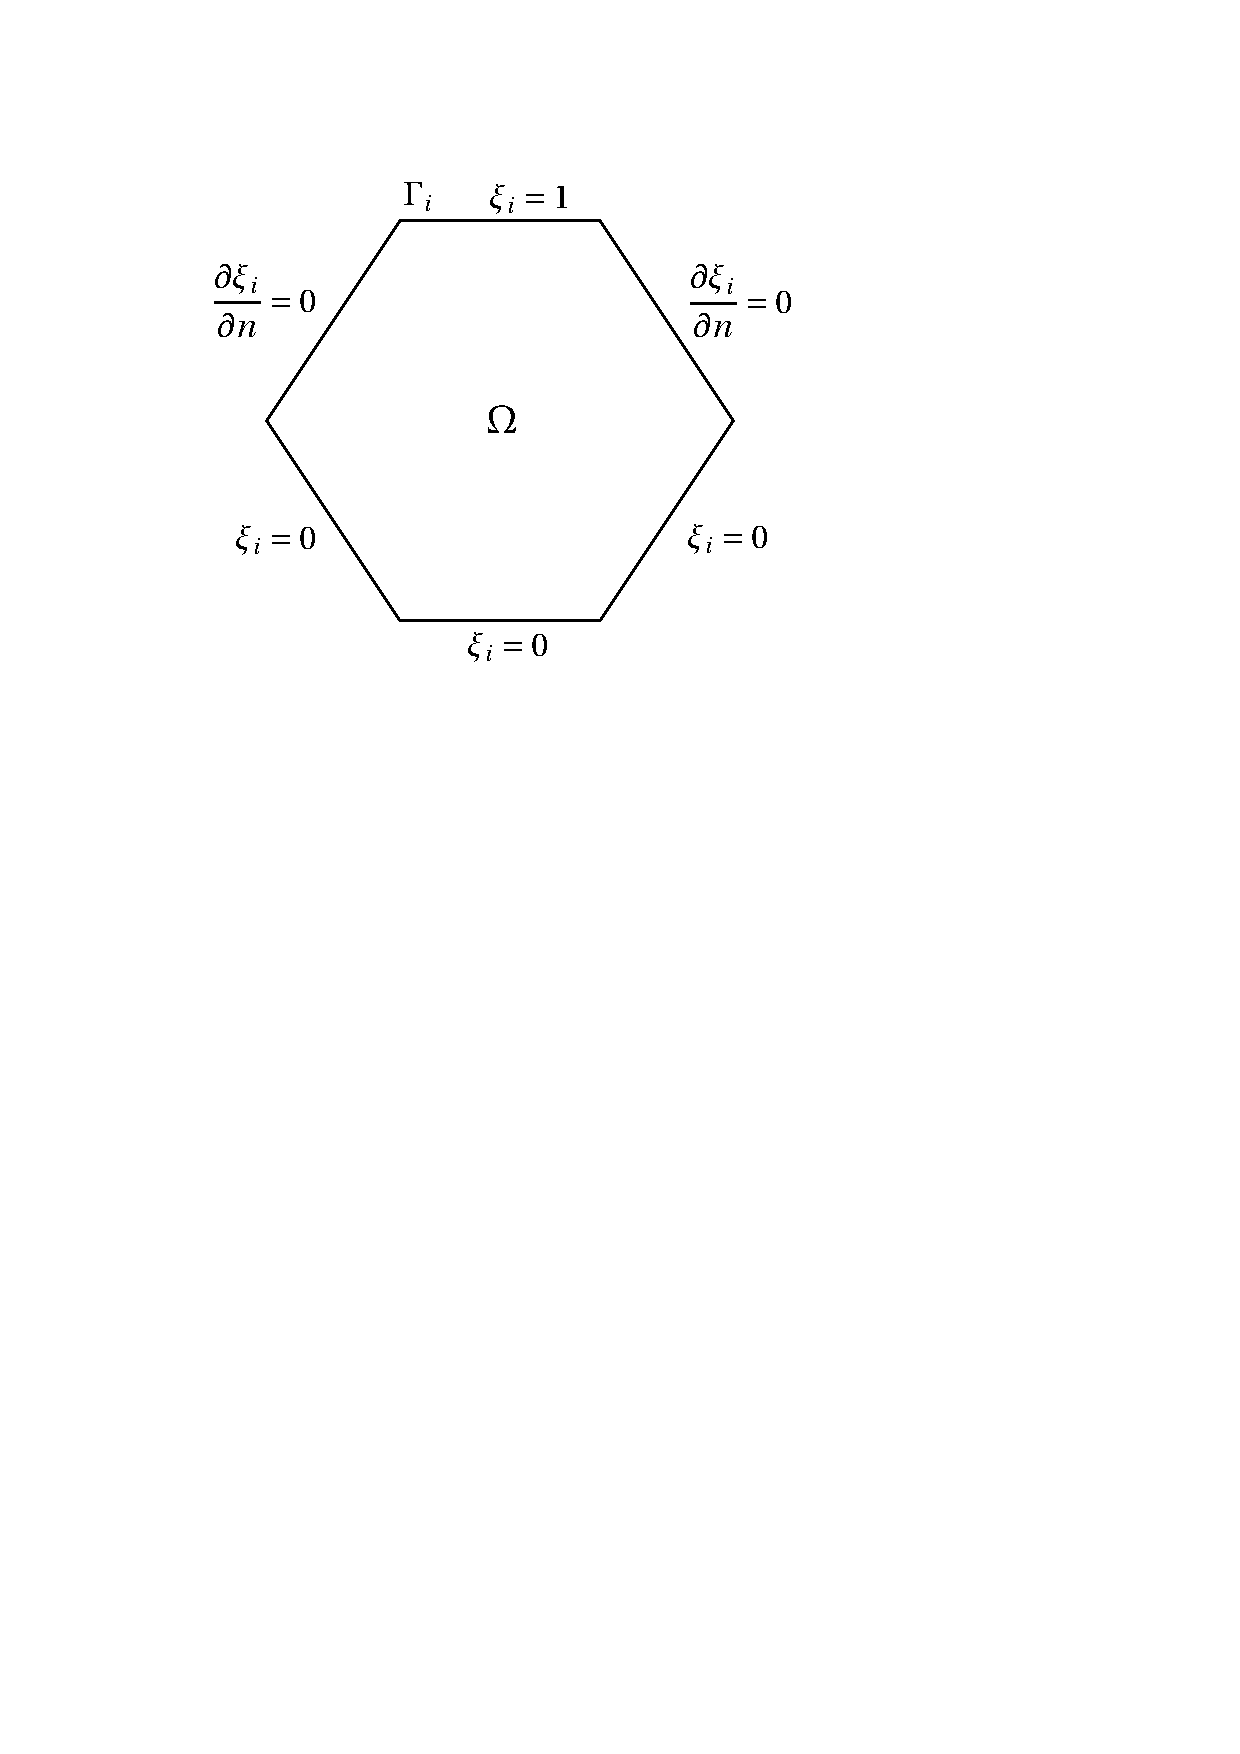
\includegraphics[scale = 0.625]{bc_weight_bis}}
			\end{minipage}
			\begin{minipage}{0.45\textwidth}
				\subfloat{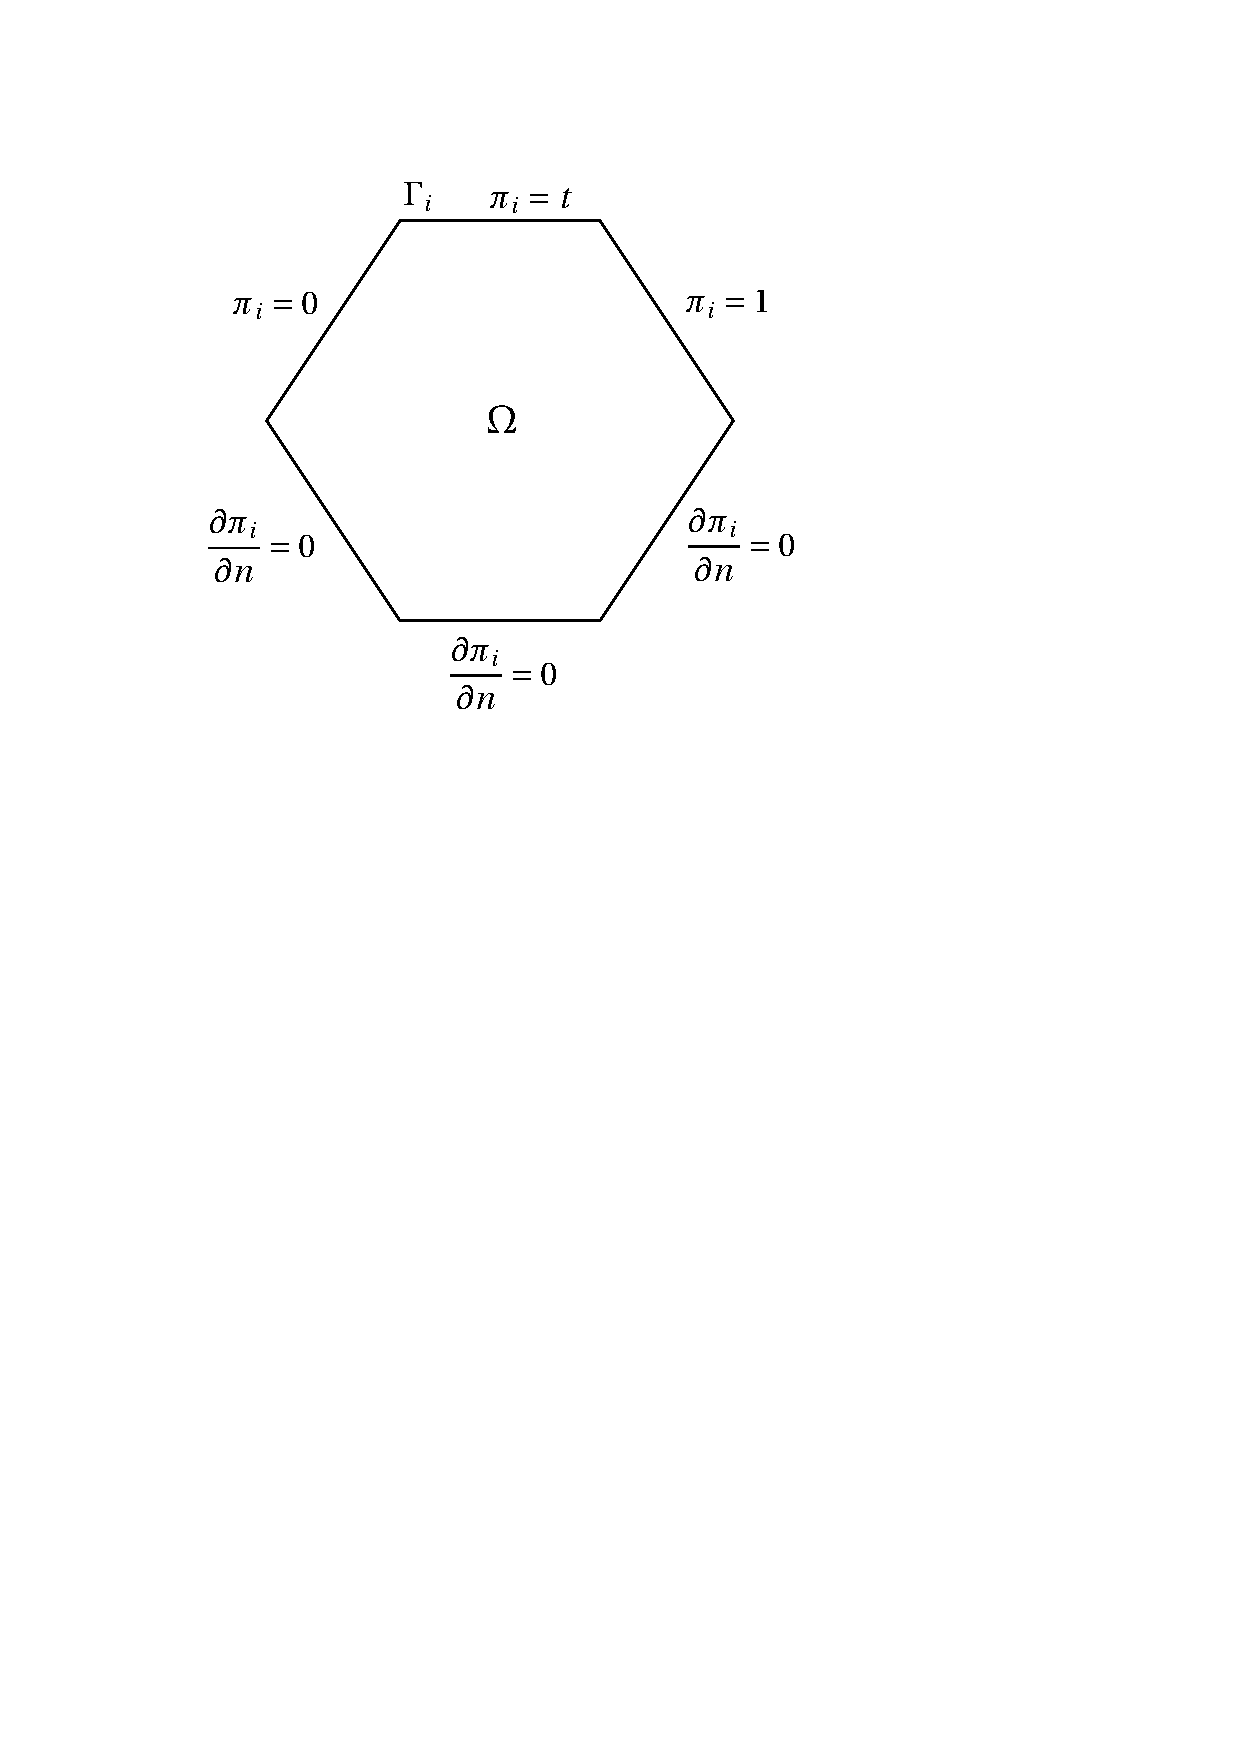
\includegraphics[scale = 0.625]{bc_proj_bis}}
			\end{minipage}
			
			\caption{Representation of the boundary conditions for the Laplace problems \eqref{eq:laplace-problem-weight-function} (\emph{left}) and \eqref{eq:laplace-problem-projection-function} (\emph{right}) stated on a exagonal reference domain $\Omega$.}
			\label{fig:laplace-bc}
		\end{figure}
	
		\begin{equation}
			\label{eq:weight-projection-function}
			\begin{aligned}
				& \xi_1 = 1 - y \, , && \xi_2 = 1 - x \, , && \xi_3 = y \, , && \xi_4 = x \, , \\
				& \pi_1 = 1 - x \, , && \pi_2 = y \, , && \pi_3 = x \, , && \pi_4 = 1 - y \, .
			\end{aligned}
		\end{equation}
		Finally, given any parameter vector $\bg{\mu} \in \mathcal{P}_g$, the boundary displacement-dependent transfinite map $\bg{\Phi} ~ : ~ \Omega \times \mathcal{P}_g \rightarrow \wt{\Omega}$ is constructed as \cite{JIR14}:
		\begin{equation}
			\label{eq:bddtm}
			\bg{\Phi}(\bg{x}; \, \bg{\mu}_g) = \bg{x} + \sum_{i = 1}^{n} \left[ \xi_i(\bg{x}) ~ \bg{d}_i(\pi_i(\bg{x}; \, \bg{\mu}_g); \, \bg{\mu}) - \xi_i(\bg{x}) ~ \xi_{i+1}(\bg{x}) ~ \bg{d}_i(1; \, \bg{\mu}_g) \right] \, ,
		\end{equation}  
		with $\xi_{n+1} = \xi_1$. Observe that, for each edge $\Gamma_i$, $i = 1, \, \ldots \, , n$, the associated displacement function is evaluated at the corresponding projection function $\pi_i$, which ranges in between $0$ and $1$ due to the maximum principle applied to the elliptic boundary value problem \eqref{eq:laplace-problem-projection-function} \cite{Rud64}. In our case, inserting \eqref{eq:weight-projection-function} into \eqref{eq:bddtm} yields:
		\begin{equation}
			\label{eq:my-bddtm}
			\begin{aligned}
				\bg{\Phi}(\bg{x}; \, \bg{\mu}_g) = \bg{x} & + (1-y) ~ \bg{d}_1(1-x; \, \bg{\mu}_g) - (1-y) ~ (1-x) ~ \bg{d}_1(1; \, \bg{\mu}_g) \\
				& + (1-x) ~ \bg{d}_2(y; \, \bg{\mu}_g) - (1-x) ~ y ~ \bg{d}_2(1; \, \bg{\mu}_g) \\
				& + y ~ \bg{d}_3(x; \, \bg{\mu}_g) - y ~ x ~ \bg{d}_3(1; \, \bg{\mu}_g) \\
				& + x ~ \bg{d}_4(1-y; \, \bg{\mu}_g) - x ~ (1-y) ~ \bg{d}_4(1; \, \bg{\mu}_g) \, .
			\end{aligned}
		\end{equation}
		Let us conclude this section by highlighting a couple of relevant remarks on the BDD TM \eqref{eq:bddtm}, which motivate its employment within this work. In contrast to the Gordon-Hall transfinite map, the position of the reference domain does not affect the effectiveness of BDD TM \cite{JIR14}. Moreover, in our numerical experiments the map \eqref{eq:my-bddtm} yielded regular transformed grids $\wt{\Omega}_h(\bg{\mu}_g)$ on $\wt{\Omega}(\bg{\mu}_g)$. In particular, for any tested value of $\bg{\mu}_g \in \mathcal{P}$, the mesh $\wt{\Omega}_h(\bg{\mu}_g)$ preserved the connectivity of the reference mesh $\Omega_h$, with no overlapping triangles. In other terms, the map \eqref{eq:my-bddtm} turns out to be \emph{conformal}, so that the requirements \ref{first-compatibility-condition} and \ref{second-compatibility-condition} are automatically fulfilled. 
		
		\begin{figure}[t]
			\center
			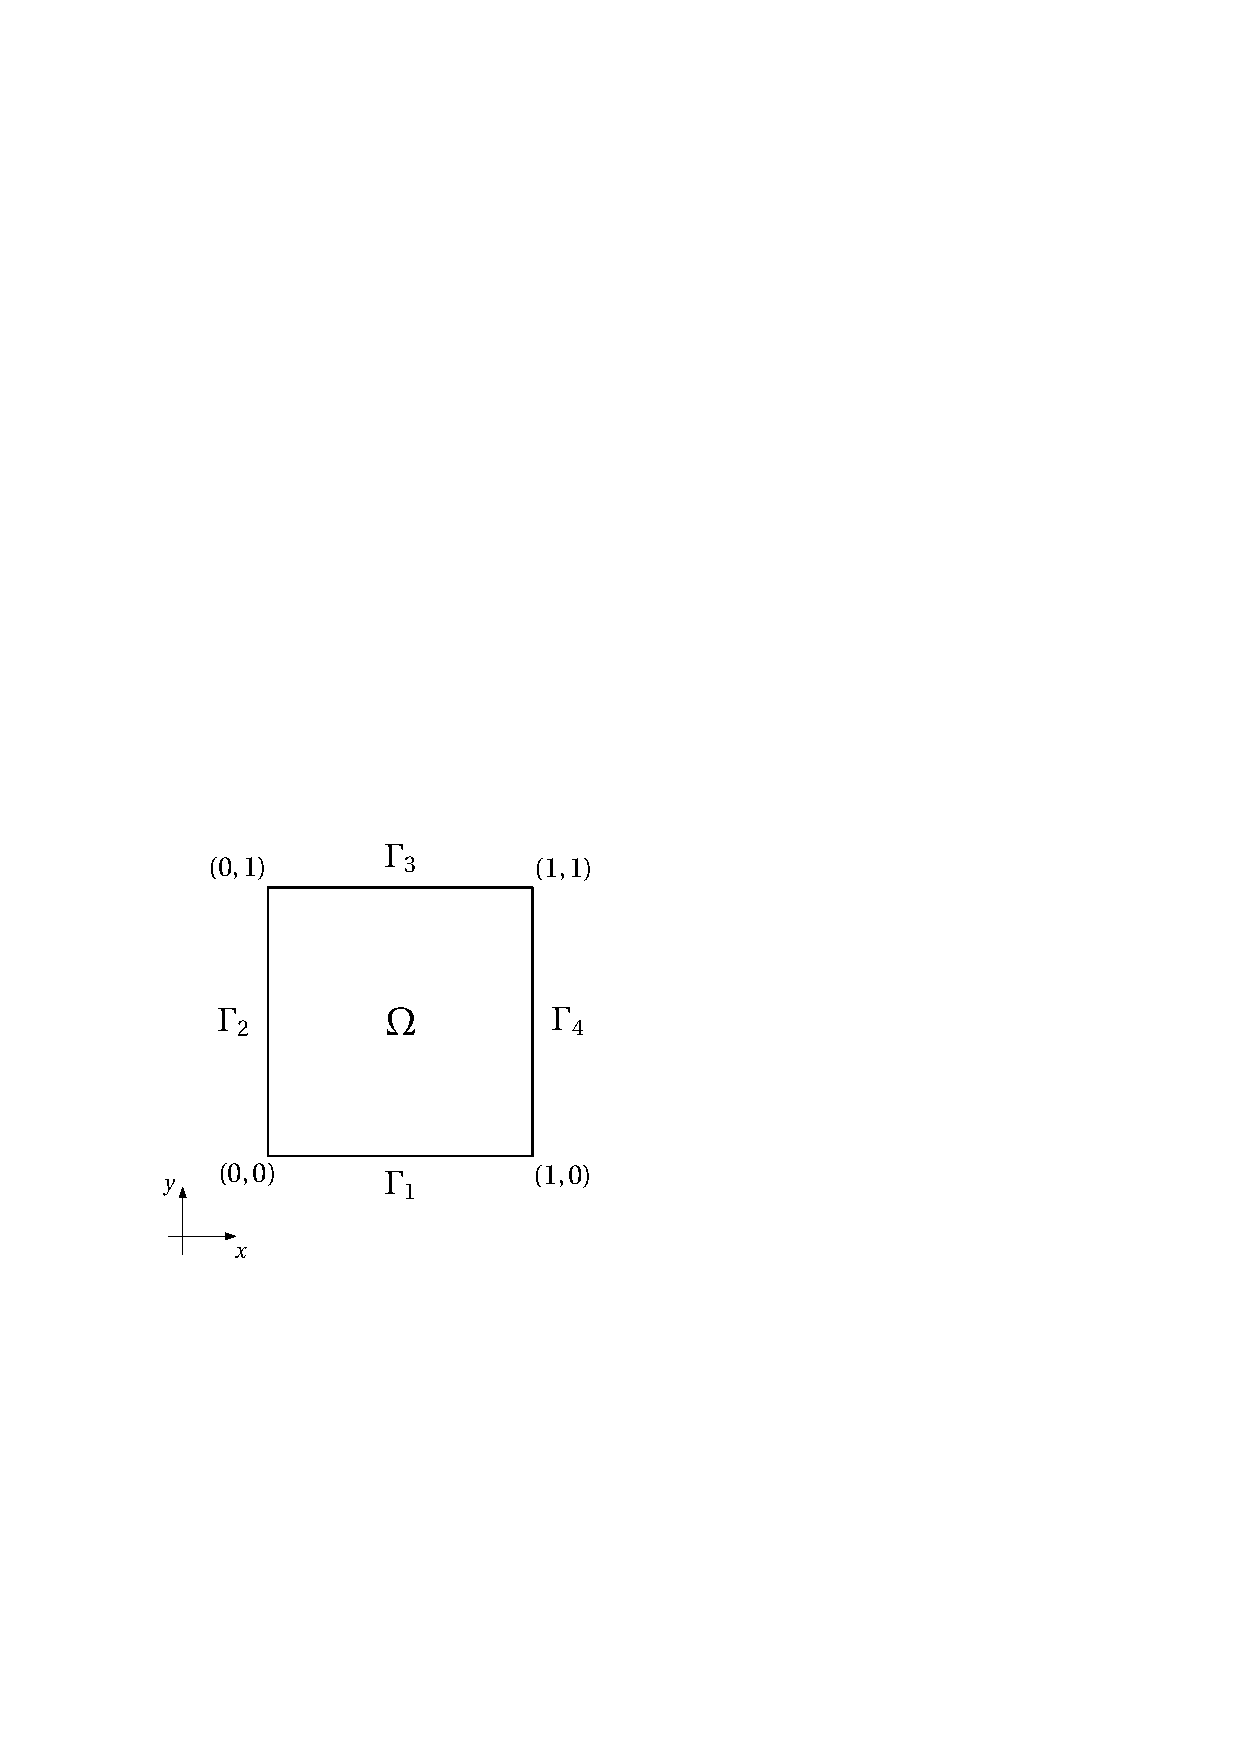
\includegraphics[scale = 0.725]{bc_square}
			
			\caption{Clockwise enumeration for the edges of the reference squared domain $\Omega$ used in the numerical tests. The coordinates of the vertices are reported too.}
			\label{fig:bc-square}
		\end{figure}
		
	\vspace*{0.3cm}
	
	\section{Well-posedness of the test cases}
	\label{section:Well-posedness of the test cases}
	
		Before proceeding with the discretization of the general problem \eqref{eq:pde-weak-reference} formulated over the reference domain $\Omega$, let us briefly investigate the well-posedness for the two examples considered in this work. In the following, we simply state the main requirements on the equations and the domain which ensure the existence and uniqueness of a weak solution. For a deeper analysis and rigorous proofs, we refer the reader to the references hereunder. We should also point out that the results we provide in this section rely on the assumption of a sufficiently smooth transformation map $\bg{\Phi}(\cdot; \bg{\mu}_g)$. However, upon resorting to the boundary displacement-dependent transfinite map and a square reference domain, this condition is automatically fulfilled. 
		
		For the nonlinear Poisson problem \eqref{eq:poisson-weak-reference}, the solution exists and is unique provided that, for any $\bg{\mu} \in \mathcal{P}$, the viscosity $k(\cdot, \cdot; \bg{\mu}) ~ : ~ \Omega \times \mathbb{R} \rightarrow [0,\infty)$ is twice continuously differentiable with respect to its second argument, and, for any compact set $\Omega_c \subset \Omega$ and any bounded interval $I$,
		\begin{equation*}
			\begin{aligned}
				& k(\bg{x}, \, r; \, \bg{\mu}) \geq \alpha > 0 && \forall (\bg{x}, \, r) \in \Omega_c \times I \, , \\
				& \Big\lvert \dfrac{\partial^q k}{\partial r^q}(\bg{x}, \, r; \, \bg{\mu}) \Big\rvert < \gamma_q \hspace*{0.3cm} && \text{for} \,\, q = 0, \, 1, \, 2, \, \, \forall (\bg{x}, \, r) \in \Omega_c \times I \, .
			\end{aligned}
		\end{equation*}
		Here, $\alpha$, $\gamma_0$, $\gamma_1$ and $\gamma_2$ are real positive constants. Moreover, we recall that, for the weak formulation to be well-defined, $s \in L^2(\Omega)$ and $g_D \in H^{1/2}(\Gamma_D)$ must hold as well. A complete proof of this result is offered in, e.g., \cite{CR97}.
		
		Conversely, to ensure the existence of a weak solution over $\Omega$ for the boundary value problem \eqref{eq:ns-differential} for the Navier-Stokes equations, we simply require the domain $\Omega$ to be Lipschitz \cite{QMN15}. Whereas, uniqueness is guaranteed upon a \emph{small data} hypothesis on the boundary conditions and a possible forcing term \cite{ESW04}. 
		
	\vspace*{0.3cm}
		
	\section{Finite element method}
	\label{section:Finite element method}
	
		In this section, we address the discretization of the parametrized problem \eqref{eq:pde-weak-reference} via the finite element (FE) method. Here, the basic ideas behind the FE strategy, an analysis of the well-posedness of the discrete problem, and a derivation of the algebraic form of the method are provided. For a comprehensive and detailed overview on finite elements, we refer the reader to, e.g., \cite{Qua10}.
		
		Let $V_h \subset V$ be a finite-dimensional subspace of $V$ of dimension $M$. The FE approximation of the weak problem \eqref{eq:pde-differential-reference} can be cast in the form: given $\bg{\mu} \in \mathcal{P}$, find $u_h(\bg{\mu}) \in V_h$ such that 
		\begin{equation}
			\label{eq:galerkin}
			g(u_h(\bg{\mu}), \, v_h; \, \bg{\mu}) = 0 \hspace*{0.3cm} \forall v_h \in V_h \, .
		\end{equation}
		The discretization \eqref{eq:galerkin} is known as \emph{Galerkin approximation}, and therefore $u_h(\bg{\mu})$ is referred to as the \emph{Galerkin solution} to the problem \eqref{eq:pde-differential-reference}. To study the well-posedness of \eqref{eq:galerkin}, consider the map $G ~ : ~ V \times \mathcal{P} \rightarrow V'$ representing our (nonlinear) differential operator, and denote by $D_u G(z, \, \bg{\mu}) ~ : ~ V \rightarrow V'$ its partial Frech\'et derivative at $(z, \, \bg{\mu}) \in V \times \mathcal{P}$, i.e., a linear bounded operator such that \cite{Rud64}
		\begin{equation*}
			\lim_{\delta z \to 0} \dfrac{\norm{G(z + \delta z; \, \bg{\mu}) - G(z; \, \bg{\mu}) - D_u G(z, \, \bg{\mu})\delta z}_{V'}}{\norm{\delta z}_V}  = 0 \, .
		\end{equation*}
		Here, $\norm{\cdot}_V$ and $\norm{\cdot}_{V'}$ denote suitable norms over $V$ and $V'$, respectively. Moreover, we denote by
		\begin{equation*}
			dg[z](w, \, v; \, \bg{\mu}) = \langle D_u G(z, \, \bg{\mu}) w, \, v \rangle \hspace*{0.3cm} \forall w, \, v \in V
		\end{equation*}
		the partial Frech\'et derivative of $g(\cdot, \cdot; \bg{\mu})$ with respect to its first argument and evaluated at $z \in V$. Then, the Galerkin problem \eqref{eq:galerkin} admits a unique solution $u_h(\bg{\mu}) \in V_h$ provided that the map $dg[u_h(\bg{\mu})](\cdot,\cdot; \bg{\mu})$ is \emph{continuous}, i.e., there exists a constant $\gamma_0 < \infty$ such that
		\begin{equation}
			\label{eq:continuity}
			\gamma(\bg{\mu}) = \sup_{w_h \in V_h} \sup_{v_h \in V_h} \dfrac{dg[u_h(\bg{\mu})](w_h, \, v_h; \, \bg{\mu})}{\norm{w_h}_V \norm{v_h}_V} \leq \gamma_0 \, ,
		\end{equation}
		and \emph{weakly coercive} (or \emph{inf-sup stable}), i.e., there exists a constant $\beta_0 > 0$ such that
		\begin{equation}
			\label{eq:inf-sup}
			\beta(\bg{\mu}) = \inf_{w_h \in V_h} \sup_{v_h \in V_h} \dfrac{dg[u_h(\bg{\mu})](w_h, \, v_h; \, \bg{\mu})}{\norm{w_h}_V \norm{v_h}_V} \geq \beta_0 \, .
		\end{equation}
		In the following, we generally assume that both \eqref{eq:continuity} and \eqref{eq:inf-sup} hold; yet in Section \ref{section:Steady Navier-Stokes equations (FE)}, we further investigate the implications of the latter requirement, known as the \emph{inf-sup condition}, on the design of a stable finite element solver for the Navier-Stokes equations.
		
		In order to solve the nonlinear Galerkin problem \eqref{eq:galerkin}, one has to resort to some iterative method, e.g., Newton's method. Starting from an initial guess $u_h^0(\bg{\mu})$, we construct a collection of approximations $\big\lbrace u_h^k(\bg{\mu}) \big\rbrace_{k \geq 0}$ to the Galerkin solution $u_h(\bg{\mu})$ by iteratively solving the linearized problems
		\begin{equation*}
			\label{eq:newton-linearized-problem}
			dg \big[ u_h^k(\bg{\mu}) \big](\delta u_h^k(\bg{\mu}), \, v_h; \, \bg{\mu}) = - g(u_h^k(\bg{\mu}), \, v_h; \, \bg{\mu}) \hspace*{0.3cm} \forall v_h \in V_h
		\end{equation*}
		in the unknown $\delta u_h^k(\bg{\mu}) \in V_h$, and then setting $u_h^{k+1}(\bg{\mu}) = u_h^k(\bg{\mu}) + \delta u_h^k(\bg{\mu})$. 
		
		To derive the algebraic counterpart of the Galerkin-Newton method, let $\big\lbrace \phi_1, \, \ldots \, , \phi_M \big\rbrace$ be a basis for the $M$-dimensional space $V_h$, so that the solution $u_h(\bg{\mu})$ can be expressed as a linear combination of the basis functions, i.e.,
		\begin{equation}
			\label{eq:galerkin-solution}
			u_h(\bg{x}; \, \bg{\mu}) = \sum_{j = 1}^M u_h^{(j)}(\bg{\mu}) ~ \phi_j(\bg{x}) \, .
		\end{equation} 
		Hence, denoting by $\mathbf{u}_h(\bg{\mu}) \in \mathbb{R}^M$ the vector collecting the \emph{degrees} \emph{of} \emph{freedom} $\big\lbrace u_h^{(j)} \big\rbrace_{j = 1}^M$ and exploiting the linearity of $g(\cdot,\cdot; \bg{\mu})$ in the second argument, the problem \eqref{eq:galerkin} is equivalent to: given $\bg{\mu} \in \mathcal{P}$, find $\mathbf{u}_h(\bg{\mu}) \in \mathbb{R}^M$ such that
		\begin{equation*}
			\label{eq:galerkin-algebraic}
			g \left( \sum_{j = 1}^M u_h^{(j)}(\bg{\mu}) ~ \phi_j, \, \phi_i; \, \bg{\mu} \right) = 0 \hspace*{0.3cm} \forall i = 1, \, \ldots \, , M \, .
		\end{equation*}
		We observe now that the above problem can be written in compact form as
		\begin{equation}
			\label{eq:galerkin-nonlinear-system}
			\mathbf{G}_h (\mathbf{u}_h(\bg{\mu}); \, \bg{\mu}) = \bg{0} \in \mathbb{R}^M \, ,
		\end{equation}
		where the $i$-th component of the \emph{residual vector} $\mathbf{G}(\cdot; \, \bg{\mu}) \in \mathbb{R}^M$ is given by
		\begin{equation}
			\label{eq:galerkin-nonlinear-system-equation}
			\left( \mathbf{G}_h(\mathbf{u}_h(\bg{\mu}); \, \bg{\mu}) \right)_i = g \left( \sum_{j = 1}^M u_h^{(j)}(\bg{\mu}) ~ \phi_j, \, \phi_i; \, \bg{\mu} \right) \, , \hspace*{0.3cm} i = 1, \, \ldots \, , M \, .
		\end{equation}
		Then, for $k \geq 0$, the $k$-th iteration of Newton's method applied to the system \eqref{eq:galerkin-nonlinear-system} entails the resolution of the \emph{linear} system
		\begin{equation}
			\label{eq:galerkin-linear-system}
			\mathbb{J}_h \big( \mathbf{u}^k_h(\bg{\mu}); \, \bg{\mu} \big) ~ \delta \mathbf{u}^k_h(\bg{\mu}) = - \mathbf{G}_h \big( \mathbf{u}^k_h(\bg{\mu}); \, \bg{\mu} \big) \, , \hspace*{0.3cm} \delta \mathbf{u}^k_h(\bg{\mu}) \in \mathbb{R}^M \, .
		\end{equation}
		so that $\mathbf{u}^{k+1}_h(\bg{\mu}) = \mathbf{u}^k_h(\bg{\mu}) + \delta \mathbf{u}^k_h(\bg{\mu})$. Here, $\mathbb{J}_h(\cdot; \, \bg{\mu}) \in \mathbb{R}^{M \times M}$ denotes the Jacobian of the residual vector $\mathbf{G}_h(\cdot; \, \bg{\mu})$; exploiting the bilinearity of $dg[z](\cdot, \cdot; \bg{\mu})$ (resulting from the linearity of the partial Frech\'et derivative $D_u G(z, \bg{\mu})$ of $G(\cdot; \bg{\mu})$), $\mathbb{J}_h(\cdot; \, \bg{\mu})$ is defined as
		\begin{equation*}
			\left( \mathbb{J}_h \big( \mathbf{u}^k_h(\bg{\mu}); \, \bg{\mu} \big) \right)_{i,j} = dg\big[u^k_h(\bg{\mu})\big](\phi_j, \, \phi_i; \, \bg{\mu}) \, , \hspace*{0.3cm} i, \, j = 1, \, \ldots \, , M \, .
		\end{equation*}
		As mentioned above, the finite element method fits the discrete and algebraic framework presented so far, entailing a precise choice for the discrete space $V_h$. In this respect, consider a mesh $\Omega_h$ discretizing the domain $\Omega \subset \mathbb{R}^d$ via non-overlapping segments ($d = 1$) or triangles ($d = 2$). For each element $K$ in the mesh, we denote by $h_K$ its diameter and we set $h = \max_{K \in \Omega_h} h_K$, thus motivating the subscript $h$ used so far to decorate any discrete variable. The FE spaces consist of globally continuous functions which are polynomial of degree $r$, $r \geq 1$, over each element, namely
		\begin{equation*}
			X_h^r = \big\lbrace v_h \in C^0 ( \overline{\Omega} ) ~ : ~ v_h \big\rvert_K \in \mathbb{P}^r(K) \hspace*{0.3cm} \forall K \in \Omega_h \big\rbrace \, , \hspace*{0.3cm} r = 1, \, 2, \, \ldots \, ,
		\end{equation*}
		with $\mathbb{P}^r(K)$ the space of polynomials of order $r$ over the element $K$. Note that $X_h^r \subset H^1(\Omega)$ for any $r$, since any $v_h \in X_h^r$ is continuous and non-differentiable in a finite number of points \cite{QMN15}. Therefore, an approximation to the unknown field
		\begin{equation}
			\label{eq:notation-1}
			u = \left( u_1, \, \ldots \, , u_S \right) \in V = V_1 \times \ldots \times V_S \subset \left[ H^1(\Omega) \right]^S
		\end{equation}  
		satisfying the differential problem \eqref{eq:pde-weak-reference} is sought in the discrete space
		\begin{equation}
			\label{eq:notation-2}
			V_h = \left( V_1 \cap X_h^{r_1} \right) \times \ldots \times \left( V_S \cap X_h^{r_S} \right) \, .
		\end{equation}
		In other terms, we seek an approximation to the generic scalar variable $u_k$, $k = 1, \, \ldots \, , S$, in a FE space properly modified to take the boundary conditions into account. It is worth pointing out that such an approximation can be made as accurate as desired, either decreasing $h$ (i.e., refining the underlying mesh) or increasing the order $r_k$ of the interpolating polynomials, possibly through adaptive strategies \cite{Qua10}. 
		
		To define a convenient basis for $X_h^r$, we introduce a set of points $\big\lbrace \bg{N}_i \big\rbrace_{i = 1}^M$, called \emph{nodes}, which form a superset of the \emph{vertices} of $\Omega_h$. Upon requiring that
		\begin{equation*}
			\phi_j(\bg{N}_i) = \delta_{ij} \hspace*{0.3cm} \forall i, \, j = 1, \, \ldots \, , M \, ,
		\end{equation*}
		with $\delta_{ij}$ the Kronecker symbol, each basis function $\phi_j$ is characterized by a \emph{local} support, overlapping the supports of a small number of other basis functions. Moreover
		\begin{equation*}
			v_h(\bg{N}_i) = v_h^{(i)} \hspace*{0.5cm} \forall i = 1, \, \ldots \, , M, \, \forall v_h \in X_h^r \, .
		\end{equation*}
		In the following, we limit ourselves to either \emph{linear} ($r = 1$) or \emph{quadratic} ($r = 2$) finite elements. In the former case, the nodes coincide with the vertices of $\Omega_h$, while in the latter the vertices are augmented with the mid-points of the edges in the mesh. 
		
		Below, we give further details on the algebraic formulation of the FE discretization for the Poisson equation and the steady Navier-Stokes equations.
		
		\begin{algorithm}[t]	
			\begin{algorithmic}[1]
				\Function{$\mathbf{u}_h = $ Newton}{$\bg{\mu}$, ~ $\Omega_h$, ~ $\mathbf{u}_h^0$, ~ $\big\lbrace \xi_i \big\rbrace_{i = 1}^n$, ~ $\big\lbrace \pi_i \big\rbrace_{i = 1}^n$, ~ $\delta$, ~ $K_{max}$}
					\State build the transformation map $\bg{\Phi}(\bg{x}; \, \bg{\mu})$ via Eq. \eqref{eq:bddtm}
					\State $k = 0$
					\DoWhile
						\State evaluate the residual vector $\mathbf{G}_h \big(\mathbf{u}_h^k ; \, \bg{\mu} \big)$
						\State form the Jacobian $\mathbb{J}_h \big(\mathbf{u}_h^k ; \, \bg{\mu} \big)$
						\State solve $\mathbb{J}_h \big(\mathbf{u}_h^k ; \, \bg{\mu} \big) ~ \delta \mathbf{u}_h^k = - \mathbf{G}_h\big(\mathbf{u}_h^k ; \, \bg{\mu} \big)$
						\State set $\mathbf{u}_h^{k+1} = \mathbf{u}_h^k + \delta \mathbf{u}_h^k$
						\State $k \leftarrow k + 1$
					\EndDoWhile{$k < K_{max}$ and $\norm{\mathbf{G}_h \big( \mathbf{u}_h^k \big)} > \delta$}
					\State $\mathbf{u}_h = \mathbf{u}_h^k$				
				\EndFunction
			\end{algorithmic}
			
			\caption{Newton's method applied to the nonlinear system \eqref{eq:galerkin-nonlinear-system}.}
			\label{alg:newton-full}
		\end{algorithm}
		
	\vspace*{0.3cm}
		 
	\subsection{Nonlinear Poisson equation}
	\label{section:Nonlinear Poisson equation (FE)}
	
		Let $V_h = X_h^1 \cap H^1_{\Gamma_D}(\Omega)$. Recalling \eqref{eq:poisson-weak-forms-reference}, the Frech\'et derivative $dg[z](\cdot, \cdot; \, \bg{\mu})$ of $g(\cdot, \cdot; \, \bg{\mu})$ is given by
		\begin{equation*}
			\begin{aligned}
			dg[z](w, \, v; \, \bg{\mu}) = \int_{\Omega} \big[ & k_r \big( z + l(\bg{\mu}); \, \bg{\mu} \big) \mathbb{J}^{-T}_{\bg{\Phi}} \nabla w \cdot \mathbb{J}^{-T}_{\bg{\Phi}} \nabla v ~ z + k \big( z + l(\bg{\mu}); \, \bg{\mu} \big) \mathbb{J}_{\bg{\Phi}}^{-T} \nabla z \cdot \mathbb{J}^{-T}_{\bg{\Phi}} \nabla v \\
			& + k_r \big(z + l(\bg{\mu}); \, \bg{\mu} \big) \mathbb{J}^{-T}_{\bg{\Phi}} \nabla l(\bg{\mu}) \cdot \mathbb{J}^{-T}_{\bg{\Phi}} \nabla v ~ w \big] \, d\Omega \, ,
			\end{aligned}
		\end{equation*} 
		where $k_r(\cdot, \cdot; \bg{\mu}) ~ : ~ \Omega \times \mathbb{R} \rightarrow \mathbb{R}$ is the partial derivative of $k(\cdot, \cdot; \, \bg{\mu})$ with respect to its second argument. Then, introducing the discrete lifting function $l_h(\bg{x}; \bg{\mu}) \in X_h^1$, obtained via, e.g., interpolation of the boundary conditions over the linear finite element space $X_h^1$, for any $\bg{\mu} \in \mathcal{P}$ the residual vector $\mathbf{G}_h(\mathbf{u}_h(\bg{\mu}); \bg{\mu})$ reads
		\begin{equation}
			\label{eq:poisson-residual-vector}
			\begin{aligned}
				\left( \mathbf{G}_h(\mathbf{u}_h(\bg{\mu}); \, \bg{\mu}) \right)_i = & \sum_{K \in \Omega_h} \Big\lbrace \sum_{j = 1}^n u_h^{(j)}(\bg{\mu}) \int_K k \big( u_h(\bg{\mu}) + l_h(\bg{\mu}); \, \bg{\mu} \big) \mathbb{J}^{-T}_{\bg{\Phi}}(\bg{\mu}) \nabla \phi_j \cdot \mathbb{J}^{-T}_{\bg{\Phi}}(\bg{\mu}) \nabla \phi_i ~ |\mathbb{J}_{\bg{\Phi}}(\bg{\mu})| \, d K \\
				& + \int_K k \big( u_h(\bg{\mu}) + l_h(\bg{\mu}); \, \bg{\mu} \big) \mathbb{J}^{-T}_{\bg{\Phi}}(\bg{\mu}) \nabla l_h(\bg{\mu}) \cdot \mathbb{J}^{-T}_{\bg{\Phi}}(\bg{\mu}) \nabla \phi_i ~ |\mathbb{J}_{\bg{\Phi}}(\bg{\mu})| \, d K \\
				& - \int_K s(\bg{\mu}) \phi_i ~ |\mathbb{J}_{\bg{\Phi}}(\bg{\mu})| \, d K \Big\rbrace \, , 
			\end{aligned}
		\end{equation}
		for all $i = 1, \, \ldots \, , M$, with its Jacobian $\mathbb{J}_h(\mathbf{u}_h(\bg{\mu}); \bg{\mu})$ given by
		\begin{equation}
			\label{eq:poisson-jacobian}
			\begin{aligned}
				\left( \mathbb{J}_h(\mathbf{u}_h(\bg{\mu}); \bg{\mu}) \right)_{i,j} = & \sum_{K \in \Omega_h} \Big\lbrace \sum_{l = 1}^M u_h^{(l)} \int_K k_r \big(u_h(\bg{\mu}) + l_h(\bg{\mu}); \, \bg{\mu} \big) \mathbb{J}^{-T}_{\bg{\Phi}}(\bg{\mu}) \nabla \phi_l \cdot \mathbb{J}^{-T}_{\bg{\Phi}}(\bg{\mu}) \nabla \phi_i ~ \phi_j ~ |\mathbb{J}_{\bg{\Phi}}(\bg{\mu})| \, dK \\
				& + \int_K k \big( u_h(\bg{\mu}) + l_h(\bg{\mu}); \bg{\mu} \big) \mathbb{J}^{-T}_{\bg{\Phi}}(\bg{\mu}) \nabla \phi_j \cdot \mathbb{J}^{-T}_{\bg{\Phi}}(\bg{\mu}) \nabla \phi_i ~ |\mathbb{J}_{\bg{\Phi}}(\bg{\mu})| \, dK \\
				& + \int_K k_r \big(u_h(\bg{\mu}) + l_h(\bg{\mu}); \, \bg{\mu} \big) \mathbb{J}^{-T}_{\bg{\Phi}}(\bg{\mu}) \nabla l_h(\bg{\mu}) \cdot \mathbb{J}^{-T}_{\bg{\Phi}}(\bg{\mu}) \nabla \phi_i ~ \phi_j ~ |\mathbb{J}_{\bg{\Phi}}(\bg{\mu})| \, dK \Big\rbrace \, , 
			\end{aligned}
		\end{equation}
		for any $i$, $j = 1, \, \ldots \, , M$. Observe that in \eqref{eq:poisson-residual-vector} and \eqref{eq:poisson-jacobian} any global integral has been split in the sum of the integrals over each element. Indeed, FE functions are continuously differentiable (actually $C^{\infty}$) on each element but not globally, due to their piecewise definition. Moreover, one typically needs a quadrature rule to compute the integrals, due to the general nonlinearity of the diffusion coefficient $k$ and the transformation map $\bg{\Phi}$. Clearly, these considerations hold also for the FE discretization of the Navier-Stokes equations.
		
	\subsection{Steady Navier-Stokes equations}
	\label{section:Steady Navier-Stokes equations (FE)}
	
		It is well-known that for the Navier-Stokes equations a suitable choice of the FE spaces is crucial to fulfill the inf-sup stability condition \eqref{eq:inf-sup} \cite{Ran99}, which for the particular case of the Navier-Stokes equations can be expressed as
		\begin{equation}
			\label{eq:inf-sup-ns}
			\beta(\bg{\mu}) = \inf_{q_h \in Q_h} \sup_{w_h \in X_h} \dfrac{b_h(q_h, \, w_h; \, \bg{\mu})}{\norm{w_h}_X \norm{v_h}_Q} \geq \beta_0 \hspace*{0.3cm} \forall \bg{\mu} \in \mathcal{P} \, ,
		\end{equation}
		where $X_h \subset X$ and $Q_h \subset Q$ are finite-dimensional approximations of the Hilbert spaces $X$ and $Q$, equipped with the norms $\norm{\cdot}_X$ and $\norm{\cdot}_Q$, respectively, and $b_h(\cdot, \cdot; \bg{\mu})$ represents a suitable discretization of the bilinear form $b(\cdot, \cdot; \bg{\mu})$ (see Eq. \eqref{eq:ns-weak-forms-b-reference}). Since the differential form \eqref{eq:ns-differential} is second order in the velocity and first order in the pressure, this suggests that the discretization of the velocity field should be richer than that one of the pressure distribution \cite{Qua10}. Therefore, a common and effective choice consists in using quadratic finite elements for the components $v_x$ and $v_y$ of the velocity and linear finite elements for the pressure, leading to the so called $\mathbb{P}^2 - \mathbb{P}^1$ (or Taylor-Hood) FE discretization \cite{Per02}. Therefore, according to the notation introduced in \eqref{eq:notation-1} and \eqref{eq:notation-2}, we have
		\begin{equation*}
			\begin{aligned}
				u = \big( v_x, \, v_y, \, p \big) \hspace*{0.3cm} \text{and} \hspace*{0.3cm} V_h = \left( X_h^2 \cap H^1_{\Gamma_D}(\Omega) \right) \times \left( X_h^2 \cap H^1_{\Gamma_D}(\Omega) \right) \times \left( X_h^1 \cap L^2(\Omega) \right) \, .
			\end{aligned}
		\end{equation*}
		Let $\big\lbrace \bg{V}_i \big\rbrace_{i = 1}^{M_v}$ be the set of vertices, associated with the linear FE basis functions $\big\lbrace \phi_i^p \big\rbrace_{i = 1}^{M_v}$ used to discretize $p$, and $\big\lbrace \bg{N}_i \big\rbrace_{i = 1}^{M_n}$ the set of nodes, associated with the quadratic FE basis functions $\big\lbrace \phi_i^{\bg{v}} \big\rbrace_{i = 1}^{M_n}$ used to discretize $\bg{v}$. Then, setting $M = 2 M_n +M_v$ and introducing the base for $V_h$
		\begin{equation*}
			\left\{ 
			\begin{bmatrix}
			\hspace*{-0.15cm}
			\begin{array}{c}
				\phi_1^{\bg{v}} \\ 
				0 \\ 
				0 
			\end{array} 
			\hspace*{-0.15cm}
			\end{bmatrix}
			\, , \, \ldots \, , 
			\begin{bmatrix}
			\hspace*{-0.15cm}
			\begin{array}{c}
				\phi_{M_n}^{\bg{v}} \\ 
				0 \\ 
				0 
			\end{array} 
			\hspace*{-0.15cm}
			\end{bmatrix}
			\, ,
			\begin{bmatrix}
			\hspace*{-0.15cm}
			\begin{array}{c}
				0 \\ 
				\phi_1^{\bg{v}} \\ 
				0 
			\end{array} 
			\hspace*{-0.15cm}
			\end{bmatrix}
			\, , \, \ldots \, ,
			\begin{bmatrix}
			\hspace*{-0.15cm}
			\begin{array}{c}
				0 \\ 
				\phi_{M_n}^{\bg{v}} \\ 
				0 
			\end{array} 
			\hspace*{-0.15cm}
			\end{bmatrix}
			\, ,
			\begin{bmatrix}
			\hspace*{-0.15cm}
			\begin{array}{c}
				0 \\ 
				0 \\ 
				\phi_1^{p} 
			\end{array} 
			\hspace*{-0.15cm}
			\end{bmatrix}
			\, , \, \ldots \, ,
			\begin{bmatrix}
			\hspace*{-0.15cm}
			\begin{array}{c}
				0 \\ 
				0 \\ 
				\phi_{M_v}^{p} 
			\end{array} 
			\hspace*{-0.15cm}
			\end{bmatrix}
			\right\} \, ,
		\end{equation*}
		for a given $\bg{\mu} \in \mathcal{P}$, the FE solution $u_h(\bg{x}; \, \bg{\mu})$ has the form
		\begin{equation*}
			u_h(\bg{x}; \, \bg{\mu}) = 
			\begin{bmatrix}
			\hspace*{-0.15cm}
			\begin{array}{c}
				v_{x,h}(\bg{x}; \, \bg{\mu}) \\
				v_{y,h}(\bg{x}; \, \bg{\mu}) \\
				p_{h}(\bg{x}; \, \bg{\mu})
			\end{array} 
			\hspace*{-0.15cm}
			\end{bmatrix}
			= \sum_{j = 1}^{M_n} v_{x,h}^{(j)}(\bg{\mu}) 
			\begin{bmatrix}
			\hspace*{-0.15cm}
			\begin{array}{c}
				\phi_j^{\bg{v}}(\bg{x}) \\ 
				0 \\ 
				0 
			\end{array} 
			\hspace*{-0.15cm}
			\end{bmatrix}
			+
			\sum_{j = 1}^{M_n} v_{y,h}^{(j)}(\bg{\mu}) 
			\begin{bmatrix}
			\hspace*{-0.15cm}
			\begin{array}{c}
				0 \\
				\phi_j^{\bg{v}}(\bg{x}) \\  
				0 
			\end{array} 
			\hspace*{-0.15cm}
			\end{bmatrix}
			+
			\sum_{j = 1}^{M_v} p_h^{(j)}(\bg{\mu})
			\begin{bmatrix}
			\hspace*{-0.15cm}
			\begin{array}{c}
				0 \\
				0 \\  
				\phi_j^{p}(\bg{x}) 
			\end{array} 
			\hspace*{-0.15cm}
			\end{bmatrix} \, .
		\end{equation*}
		As usual, we denote by $\mathbf{u}_h(\bg{\mu}) \in \mathbb{R}^M$ the vector collecting the degrees of freedom of $u_h(\bg{\mu})$, ordered as follows:
		\begin{equation*}
			\mathbf{u}_h(\bg{\mu}) = \big[ \underbrace{v_{x,h}^{(1)}(\bg{\mu}), \, \ldots \, , v_{x,h}^{(M_n)}(\bg{\mu}), \, v_{y,h}^{(1)}(\bg{\mu}), \, \ldots \, , v_{y,h}^{(M_n)}(\bg{\mu})}_{\mathbf{v}_h(\bg{\mu})^T \in \mathbb{R}^{2 M_n}}, \, \underbrace{p_h^{(1)}(\bg{\mu}), \, \ldots \, , p_h^{(M_v)}(\bg{\mu})}_{\mathbf{p}_h(\bg{\mu})^T \in \mathbb{R}^{M_v}} \big]^T \, .
		\end{equation*}
		Moreover, in view of the following computations, let us also introduce a basis $\big\lbrace \bg{\phi}_1, \, \ldots \, , \bg{\phi}_{2 M_n} \big\rbrace$ for the velocity trial and test space, with, for $j = 1, \, \ldots \, , M_n$,
		\begin{equation*}
			\bg{\phi}_j = 
			\begin{bmatrix}
			\hspace*{-0.15cm}
			\begin{array}{c} 
				\phi_j^{\bg{v}} \\
				0 
			\end{array} 
			\hspace*{-0.15cm}
			\end{bmatrix} 
			\hspace*{0.5cm} \text{and} \hspace*{0.5cm} \bg{\phi}_{M_n + j} = 
			\begin{bmatrix}
			\hspace*{-0.15cm}
			\begin{array}{c} 
				0 \\
				\phi_j^{\bg{v}}  
			\end{array} 
			\hspace*{-0.15cm}
			\end{bmatrix} \, ,
		\end{equation*}
		so that
		\begin{equation*}
			\begin{aligned}
			\bg{v}_h(\bg{x}; \, \bg{\mu}) & = \sum_{j = 1}^{M_n} \left( v_{x,h}^{(j)}(\bg{\mu}) ~ \bg{\phi}_{j}(\bg{x}) + v_{y,h}^{(j)}(\bg{\mu}) ~ \bg{\phi}_{M_n + j}(\bg{x}) \right) \\
			& = \sum_{j = 1}^{M_n} \left( u_h^{(j)}(\bg{\mu}) ~ \bg{\phi}_{j}(\bg{x}) + u_h^{(M_n + j)}(\bg{\mu}) ~ \bg{\phi}_{M_n + j}(\bg{x}) \right) \, .
			\end{aligned}
		\end{equation*}
		Given \eqref{eq:ns-weak-reference}, \eqref{eq:ns-weak-forms} and \eqref{eq:galerkin-nonlinear-system-equation}, the residual vector for the Navier-Stokes equations is defined as (we omit the dependence on $\bg{\mu}$ to ease the notation): 
		\begin{equation*}
			\begin{aligned}
				&
				\begin{aligned}
					\left( \mathbf{G}_h(\mathbf{u}_h; \, \bg{\mu}) \right)_i = & \sum_{j = 1}^{2 M_n} v_h^{(j)} \left[ a_h(\bg{\phi}_j, \, \bg{\phi}_i; \, \bg{\mu}) + d_h(\bg{\phi}_j, \, \bg{\phi}_i; \, \bg{\mu}) \right] + \sum_{j = 1}^{2 M_n} \sum_{k = 1}^{2 M_n} v_h^{(j)} v_h^{(k)} c_h(\bg{\phi}_j, \, \bg{\phi}_k, \, \bg{\phi}_i; \, \bg{\mu}) \\
					& + \sum_{q = 1}^{M_v} p_h^{(q)} b_h(\phi_q^p, \, \bg{\phi}_i; \, \bg{\mu}) - f_{1 h}(\bg{\phi}_i; \, \bg{\mu}) \hspace*{1.525cm} \text{for $i = 1, \, \ldots \, 2 M_n$} \, ,
				\end{aligned} \\
				& \left( \mathbf{G}_h(\mathbf{u}_h; \, \bg{\mu}) \right)_{2 M_n + q} = \sum_{j = 1}^{2 M_n} v_h^{(j)} b_h(\phi_q^p, \, \bg{\phi}_j, \, ; \, \bg{\mu}) - f_{2 h}(\phi_q^p; \, \bg{\mu}) \hspace*{0.7cm} \text{for $q = 1, \, \ldots \, M_v$} \, ,
			\end{aligned}
		\end{equation*}
		with
		\begin{equation*}
			\begin{aligned}
				& a_h(\bg{\phi}_j, \, \bg{\phi}_i; \, \bg{\mu}) = \sum_{K \in \Omega_h} a_K(\bg{\phi}_j, \, \bg{\phi}_i; \, \bg{\mu}) \, , && d_h(\bg{\phi}_j, \, \bg{\phi}_i; \, \bg{\mu}) = \sum_{K \in \Omega_h} d_K(\bg{\phi}_j, \, \bg{\phi}_i; \, \bg{\mu}) \, , \\
				& c_h(\bg{\phi}_j, \, \bg{\phi}_k, \, \bg{\phi}_i; \, \bg{\mu}) = \sum_{K \in \Omega_h} c_K(\bg{\phi}_j, \, \bg{\phi}_k, \, \bg{\phi}_i; \, \bg{\mu}) \, , \hspace*{0.5cm} && b_h(\phi_q^p, \, \bg{\phi}_i; \, \bg{\mu}) = \sum_{K \in \Omega_h} b_K(\phi_q^p, \, \bg{\phi}_i; \, \bg{\mu}) \, , \\
				& f_{1 h}(\bg{\phi}_i; \, \bg{\mu}) = \sum_{K \in \Omega_h} f_{1\,K}(\bg{\phi}_i; \, \bg{\mu}) \, , && f_{2 h}(\phi_q^p; \, \bg{\mu}) = \sum_{K \in \Omega_h} f_{2\,K}(\phi_q^p; \, \bg{\mu}) \, ,
			\end{aligned}
		\end{equation*}
		where $a_K(\cdot, \cdot; \bg{\mu})$, $d_K(\cdot, \cdot; \bg{\mu})$, $c_K(\cdot, \cdot, \cdot; \bg{\mu})$, $b_K(\cdot, \cdot; \bg{\mu})$, $f_{1 K}(\cdot, \cdot; \bg{\mu})$ and $f_{2 K}(\cdot, \cdot; \bg{\mu})$ represent the restrictions of $a(\cdot, \cdot; \bg{\mu})$, $d(\cdot, \cdot; \bg{\mu})$, $c(\cdot, \cdot, \cdot; \bg{\mu})$, $b(\cdot, \cdot; \bg{\mu})$, $f_{1}(\cdot, \cdot; \bg{\mu})$ and $f_{2}(\cdot, \cdot; \bg{\mu})$, respectively, over the element $K \in \Omega_h$. Moreover, we recall that the definitions of the bilinear form $d(\cdot, \cdot; \bg{\mu})$ and the linear forms $f_1(\cdot; \bg{\mu})$ and $f_2(\cdot; \bg{\mu})$ rely on the introduction of a lifting vector $\bg{l} = \bg{l}(\bg{\mu}) \in \big[ H^1(\Omega) \big]^2$, which has then to be interpolated over the finite element space $\big[ X_h^2 \big]^2$, yielding the discrete lifting vector $\bg{l}_h = \bg{l}_h \in \big[ X_h^2 \big]^2$. \\
		Upon introducing the matrices $\mathbb{A}(\bg{\mu}) \in \mathbb{R}^{2 M_n \times 2 M_n}$, $\mathbb{C}(\mathbf{v}_h(\bg{\mu}); \, \bg{\mu}) \in \mathbb{R}^{2 M_n \times 2 M_n}$ and $\mathbb{B}(\bg{\mu}) \in \mathbb{R}^{M_v \times 2 M_n}$, and the vectors $\mathbf{f}_1(\bg{\mu}) \in \mathbb{R}^{2 M_n}$ and $\mathbf{f}_2(\bg{\mu}) \in \mathbb{R}^{M_v}$, defined as
		\begin{equation*}
			\begin{aligned}
				& \big( \mathbb{A}(\bg{\mu}) \big)_{i,j} = a_h(\bg{\phi}_j, \, \bg{\phi}_i; \bg{\mu}) + d_h(\bg{\phi}_j, \, \bg{\phi}_i; \bg{\mu}) && i, \, j = 1, \, \ldots \, , 2 M_n \, , \\
				& \big( \mathbb{C}(\mathbf{v}_h(\bg{\mu}); \, \bg{\mu}) \big)_{i,j} = \sum_{k = 1}^{2 M_n} v_h^{(k)} c_h(\bg{\phi}_j, \, \bg{\phi}_k, \, \bg{\phi}_i; \, \bg{\mu}) && i, \, j = 1, \, \ldots \, , 2 M_n \, , \\
				\label{eq:B}
				& \big( \mathbb{B}(\bg{\mu}) \big)_{q,j} = b_h(\phi_q^p, \, \nabla \cdot \bg{\phi}_j; \, \bg{\mu}) && q = 1, \, \ldots \, , M_v \, , \, j = 1, \, \ldots \, , 2 M_n \, , \\
				& \big( \mathbf{f}_1(\bg{\mu}) \big)_i = f_{1\,h}(\bg{\phi}_i; \, \bg{\mu}) && i = 1, \, \ldots \, , 2 M_n \, , \\
				& \big( \mathbf{f}_2(\bg{\mu}) \big)_q = f_{2\,h}(\phi_p^q; \, \bg{\mu}) && q = 1, \, \ldots \, , M_v \, ,
			\end{aligned}
		\end{equation*}
		the nonlinear system obtained by the FE method can be written in compact form as follows:
		\begin{equation}
			\label{eq:ns-system}
			\begin{bmatrix}
			\hspace*{-0.15cm}
			\begin{array}{cc}
				\mathbb{A}(\bg{\mu}) + \mathbb{C}(\mathbf{v}_h(\bg{\mu}); \, \bg{\mu}) & \mathbb{B}(\bg{\mu})^T \\
				\mathbb{B}(\bg{\mu}) & 0
			\end{array} 
			\hspace*{-0.15cm}
			\end{bmatrix} 
			\begin{bmatrix}
			\hspace*{-0.15cm}
			\begin{array}{c}
				\mathbf{v}_h(\bg{\mu}) \\
				\mathbf{p}_h(\bg{\mu})
			\end{array} 
			\hspace*{-0.15cm}
			\end{bmatrix} 
			=
			\begin{bmatrix}
			\hspace*{-0.15cm}
			\begin{array}{c}
				\mathbf{f}_1(\bg{\mu}) \\
				\mathbf{f}_2(\bg{\mu})
			\end{array} 
			\hspace*{-0.15cm}
			\end{bmatrix} \, .
		\end{equation}
		Hence, the Jacobian is given by:
		\begin{equation*}
			\label{eq:ns-jacobian}
			\mathbb{J}_h(\mathbf{u}_h(\bg{\mu}); \, \bg{\mu}) =
			\begin{bmatrix}
			\hspace*{-0.15cm}
			\begin{array}{cc} 
				\mathbb{A}(\bg{\mu}) + \big( \bar{\mathbb{C}}(\bg{\mu}) + \bar{\mathbb{C}}(\bg{\mu})^T \big) \, \mathbf{v}_h(\bg{\mu}) & \mathbb{B}^T(\bg{\mu}) \\
				\mathbb{B}(\bg{\mu}) & 0
			\end{array} 
			\hspace*{-0.15cm}
			\end{bmatrix} \, ,
		\end{equation*}
		where $\bar{\mathbb{C}}(\bg{\mu}) \in \mathbb{R}^{2 M_n \times 2 M_n}$ is defined as
		\begin{equation*}
			\big( \bar{\mathbb{C}}(\bg{\mu}) \big)_{i,j} = \sum_{k = 1}^{2 M_n} c_h(\bg{\phi}_j, \, \bg{\phi}_k, \, \bg{\phi}_i; \, \bg{\mu}) \hspace*{0.5cm} \text{for $i, \, j = 1, \, \ldots \, , 2 M_n$} \, .
		\end{equation*}
		
	\vspace*{0.1cm}
		
	\section{POD-Galerkin reduced basis method}
	\label{section:POD-Galerkin reduced basis method}
		
		As detailed in the previous section, the finite element discretization of the $\bg{\mu}$-dependent nonlinear differential problem \eqref{eq:pde-weak-reference}, combined with Newton's method, entails the assembly and resolution of (possibly) many linear systems of the form \eqref{eq:galerkin-linear-system}, whose dimension is directly related to $(i)$ the size of the underlying grid and $(ii)$ the order of the polynomial spaces adopted. Since the accuracy of the resulting discretization heavily relies on these two factors, a direct numerical approximation of the \emph{full order} model implies severe computational costs. Therefore, even resorting to high-performance parallel workstations, this approach is hardly affordable in \emph{many-query} and \emph{real-time} contexts, where one is interested in a fast and reliable prediction of an \emph{output of interest}, i.e, a functional of the field variable $u(\bg{\mu})$, for many instances of $\bg{\mu} \in \mathcal{P}$ \cite{Dep08}. This motivates the broad use of \emph{reduced-order} models, across several inter-disciplinary areas, e.g., parameter estimation, optimal control, shape optimization and uncertainty quantification \cite{HSR16, QMN15}. 
		
		In this work we focus on reduced basis (RB) methods for the approximation of the variational problem \eqref{eq:pde-weak-reference}. To this end, let us recall the definition of the solution manifold $\mathcal{M}$,
		\begin{equation*}
			\mathcal{M} = \big\lbrace u(\bg{\mu}) ~ : ~ \bg{\mu} \in \mathcal{P} \big\rbrace \subset V \, ,
		\end{equation*}
		and its discrete counterpart $\mathcal{M}_h$,
		\begin{equation*}
			\mathcal{M}_h = \big\lbrace u_h(\bg{\mu}) ~ : ~ \bg{\mu} \in \mathcal{P} \big\rbrace \subset V_h \, .
		\end{equation*}
		For any $\bg{\mu} \in \mathcal{P}$, we assume that the FE solution $u_h(\bg{\mu})$ can be lead as close as desired (in the $V$-norm) to the corresponding continuous solution $u_h(\bg{\mu})$ (either by refining the computational mesh or by increasing the order of the FE space), so that $\mathcal{M}_h$ provides a good approximation of $\mathcal{M}$. Hence, in the following we refer to $u_h(\bg{\mu})$ as the \emph{truth} solution.
		
		Reduced basis methods seek an approximated solution to the problem \eqref{eq:pde-weak-reference} as a linear combination of parameter-independent functions $\big\lbrace \psi_1, \, \ldots \, , \psi_L \big\rbrace \subset V_h$, called \emph{reduced basis functions}, built from a collection of high-fidelity solutions $\big\lbrace u_h \big( \bg{\mu}^{(1)} \big), \, \ldots \, , u_h \big( \bg{\mu}^{(N)} \big) \big\rbrace \subset \mathcal{M}_h$, called \emph{snapshots}, where the discrete and finite set $\Xi_N = \big\lbrace \bg{\mu}^{(1)}, \, \ldots \, , \bg{\mu}^{(N)} \big\rbrace \subset \mathcal{P}$ may consist of either a uniform lattice or randomly generated points over the parameter domain $\mathcal{P}$ \cite{HSR16}. The basis functions $\big\lbrace \psi_l \big\rbrace_{l = 1}^L$ generally follow from a principal component analysis (PCA) of the set of snapshots (in that case, $N > L$), or they might coincide with the snapshots themselves (in that case, $N = L$). In the latter approach, typical of any \emph{greedy} method, the parameters $\big\lbrace \bg{\mu}^{(n)} \big\rbrace_{n = 1}^N$ must be carefully chosen according to some optimality criterium (see, e.g., \cite{Chen17}). Here, we pursue the first approach, employing the well-known Proper Orthogonal Decomposition (POD) method \cite{Vol08}, detailed in the following subsection.
		
		Assume now that a reduced basis is available and let $V_{\texttt{rb}} \subset V_h$ be the associated \emph{reduced basis space}, i.e.,
		\begin{equation*}
			V_{\texttt{rb}} = \text{span} \big\lbrace \psi_1, \, \ldots \, , \psi_L \big\rbrace \, .
		\end{equation*} 
		A \emph{reduced basis solution} $u_{L}(\bg{\mu})$ is sought in the form
		\begin{equation}
			\label{eq:rb-solution}
			u_{L}(\bg{x}; \, \bg{\mu}) = \sum_{l = 1}^L u_{\texttt{rb}}^{(l)}(\bg{\mu}) ~ \psi_l(\bg{x}) \in V_{\texttt{rb}} \, ,
		\end{equation}
		with $\mathbf{u}_{\texttt{rb}}(\bg{\mu}) = \big[ u_{\texttt{rb}}^{(1)}(\bg{\mu}), \, \ldots \, , u_{\texttt{rb}}^{(L)}(\bg{\mu}) \big]^T \in \mathbb{R}^L$ be the \emph{coefficients} (also called \emph{generalized coordinates}) for the expansion of the RB solution in the RB basis functions. Before further proceeding with the derivation of the method, let us gain some insights into the rational behind the reduced basis approach. As one can foresee, RB methods (potentially) enable a relevant reduction in the computational effort when the dimension of the associated test and trial space $V_{\texttt{rb}}$ is significantly smaller than the dimension of the original finite element space $V_h$; in other terms, $L << M$ must hold. However, this assumes that the solution manifold $\mathcal{M} \subset V$ (or, equivalently, $\mathcal{M}_h \subset V_h$, for what previously said) is actually of low-dimension, and can then be accurately approximated by a subspace of reduced dimension $L$ \cite{HSR16}. To further investigate this necessary hypothesis, it is worth introducing the notion of Kolmogorov $L$-width. The definition is \cite{Mad06}:
		
		\begin{definition}
			\emph{
			Let $X$ be a linear space equipped with the norm $\norm{\cdot}_X$, $A$ be a subset of $X$ and $X_L$ be a generic $L$-dimensional subspace of $X$. The deviation of $A$ from $X_L$ is defined as
			\begin{equation*}
				E(A; \, X_L) = \adjustlimits \sup_{x \in A} \inf_{y \in X_L}  \norm{x - y}_X \, .
			\end{equation*}
			Then, the \emph{Kolmogorov $L$-width} of $A$ in $X$ is given by
			\begin{equation}
				\label{eq:kolmogorov-L-width}
				\begin{aligned}
					d_L(A, \, X) & = \inf \big\lbrace E(A; \, X_L) ~ : ~ \text{$X_L$ is an $L$-dimensional subspace of $X$} \big\rbrace \\
					& = \adjustlimits \inf_{X_L} \sup_{x \in A} \inf_{y \in X_L} \norm{x - y}_X \, .
				\end{aligned}
			\end{equation}
			}
		\end{definition}
		
		\noindent Therefore, $d_L(A, \, X)$ measures the extent to which the subset $A$ of the vector space $X$ can be well-approximated by an $L$-dimensional subspace \cite{Mad06}. Indeed, there exist many situations in which the Kolmogorov $L$-width shows a graceful behaviour with $L$, e.g., an exponential decay. In our case, $X = V$ and $A = \mathcal{M}$, and we can refer to regularity of the solutions $u(\bg{\mu})$ with respect to the parameter $\bg{\mu}$, or even to analyticity in the parameter dependence \cite{Buf12}.
		
		Nevertheless, we still have to ensure that the RB space $V_{\texttt{rb}}$, i.e., the chosen $X_L$ in \eqref{eq:kolmogorov-L-width}, attains the infimum $d_L(\mathcal{M}, \, V)$, or at least a value close to the infimum. At this regard, let us consider the following bound for the error committed when approximating the continuous solution $u(\bg{\mu})$ with $u_L(\bg{\mu})$:
		\begin{equation*}
			\norm{u(\bg{\mu}) - u_L(\bg{\mu})}_V \leq \norm{u(\bg{\mu}) - u_h(\bg{\mu})}_V + \norm{u_h(\bg{\mu}) - u_L(\bg{\mu})}_V \hspace*{0.3cm} \forall \bg{\mu} \in \mathcal{P} \, .
		\end{equation*}
		The first term on the right-hand side measures the discrepancy between the continuous solution and its high-fidelity approximation. For what said above, this error can be lower to any desired level of accuracy. Therefore, the reliability of the solution provided by any reduced basis technique relies on a sound control of the second term of the right-hand side $\norm{u_h(\bg{\mu}) - u_L(\bg{\mu})}_V$, i.e., the error between the truth and the reduced solution. The last decade has whitnessed the development of different \emph{a priori} and \emph{a posteriori} estimates for such error (see, e.g., \cite{Buf12, HSR16, Mad06}), thus \emph{certifying} the RB procedure, that is, enabling the user to trust the output of the RB method. However, as already mentioned, the range of application of these estimates is usually limited to linear problems with an affine dependence on the parameters. Although recent and relevant improvements have been achieved also for the Navier-Stokes equations (see, e.g., \cite{Dep08, QMN15}), they rely on non-trivial results from functional analysis and involve rather long calculations. Hence, it is not the intent of this project to further investigate and employ these estimates. Yet, in our numerical simulations we shall \emph{empirically} study the effectiveness of the proposed POD-Galerkin method by evaluating the error $\norm{u_h(\bg{\mu}) - u_L(\bg{\mu})}_V$ on a finite and discrete \emph{test} dataset $\Xi_{te} \in \mathcal{P}$. We refer the reader to Section \ref{section:A POD-based RB method using neural networks} for a deeper discussion.
		
		Let us now resume the derivation of the POD-Galerkin RB method. To unearth $u_L(\bg{\mu})$, whose general form is given in \eqref{eq:rb-solution}, we proceed to project the variational problem \eqref{eq:pde-weak-reference} onto the RB space $V_{\texttt{rb}}$ by pursuing a standard Galerkin approach, leading to the following \emph{reduced basis problem}: given $\bg{\mu} \in \mathcal{P}$, find $u_L(\bg{\mu}) \in V_{\texttt{rb}}$ so that
		\begin{equation}
			\label{eq:pde-rb}
			g(u_L(\bg{\mu}), \, v_L; \, \bg{\mu}) = 0 \hspace*{0.3cm} \forall v_L \in V_{\texttt{rb}} \, .
		\end{equation}
		Then, Newton's method applied to \eqref{eq:pde-rb} entails, at each iteration $k \geq 0$, the solution of the linearized problem: given $\bg{\mu} \in \mathcal{P}$, seek $\delta u_{L}^k(\bg{\mu})$ such that
		\begin{equation*}
			\label{eq:pde-rb-newton}
			dg \big[ u_{L}^k(\bg{\mu}) \big] \big( \delta u_{L}^k(\bg{\mu}), \, v_{L}; \, \bg{\mu} \big) = - g \big( u_{L}^k(\bg{\mu}), \, v_{L}; \, \bg{\mu} \big) \hspace*{0.3cm} \forall v_{L} \in V_{\texttt{rb}} \, ,
		\end{equation*}
		with $u_{L}^{k+1}(\bg{\mu}) = u_{L}^k(\bg{\mu}) + \delta u_{L}^k(\bg{\mu})$.
		
		Let us point out that the RB functions $\big\lbrace \psi_l \big\rbrace_{l = 1}^L$ belong to $V_h$, i.e., they are actual finite element functions. Hence, we denote by $\bg{\psi}_l \in \mathbb{R}^M$ the vector collecting the nodal values of $\psi_l$, for $l = 1, \, \ldots \, , L$, and introduce the matrix $\mathbb{V} = \big[ \bg{\psi}_1, \, \big| \, \ldots \, \big| \, , \bg{\psi}_L \big] \in \mathbb{R}^{M \times L}$. For any $v_{L} \in V_{\texttt{rb}}$, the matrix $\mathbb{V}$ encodes the change of variables from the RB basis to the standard (Lagrangian) FE basis, i.e.,
		\begin{equation}
			\label{eq:rb-fe-coefficients}
			\mathbf{v}_L = \mathbb{V} ~ \mathbf{v}_{\texttt{rb}} \, .
		\end{equation}
		Therefore, each element $v_{L}$ of the reduced space admits two (algebraic) representations:
		\begin{itemize}
			\item $\mathbf{v}_{\texttt{rb}} \in \mathbb{R}^L$, collecting the coefficients for the expansion of $v_{L}$ in terms of the RB basis $\big\lbrace \psi_1, \, \ldots \, , \psi_L \big\rbrace$;
			\item $\mathbf{v}_{L} \in \mathbb{R}^M$, collecting the coefficients for the expansion of $v_{L}$ in terms of the FE basis $\big\lbrace \phi_1, \, \ldots \, , \phi_M \big\rbrace$.
		\end{itemize}
		Note that the latter is also available for any $v_h \in V_h$, while the former characterizes the element in the subspace $V_{\texttt{rb}}$.
		
		Upon choosing $v_{L} = \psi_l$, $l = 1, \, \ldots \, , L$, in the RB problem \eqref{eq:pde-rb}, for any $\bg{\mu} \in \mathcal{P}$ we get the set of equations
		\begin{equation}
			\label{eq:rb-algebraic-formulation-1}
			g(u_{L}(\bg{\mu}), \, \psi_l; \, \bg{\mu}) = 0 \hspace*{0.3cm} 1 \leq l \leq L \, .
		\end{equation}
		Inserting into \eqref{eq:rb-algebraic-formulation-1} the expansion of $\psi_l$, $l = 1, \, \ldots \, , L$, in terms of the canonical FE basis $\big\lbrace \phi_m \big\rbrace_{m = 1}^M$, i.e.,
		\begin{equation*}
			\psi_l(\bg{x}) = \sum_{m = 1}^M \psi_l^{(m)} ~ \phi_m(\bg{x}) = \sum_{m = 1}^M \mathbb{V}_{m,l} ~ \phi_m(\bg{x}) \, ,
		\end{equation*} 
		and exploiting the linearity of $g(\cdot,\cdot; \bg{\mu})$ in the second argument, yields:
		\begin{equation*}
			0 = \sum_{m = 1}^M \mathbb{V}_{m,l} ~ g(u_L(\bg{\mu}), \, \phi_m; \, \bg{\mu}) = \big( \mathbb{V}^T \mathbf{G}_h(\mathbf{u}_L(\bg{\mu}); \bg{\mu}) \big)_l \hspace*{0.3cm} 1 \leq l \leq L \, ,
		\end{equation*}
		where the last equality follows from the definition \eqref{eq:galerkin-nonlinear-system-equation} of the residual vector $\mathbf{G}_h(\cdot; \bg{\mu})$ and the notation introduced in \eqref{eq:rb-fe-coefficients}. Then, the algebraic formulation of the reduced basis problem \eqref{eq:pde-rb} can be written in compact form as:
		\begin{equation}
			\label{eq:rb-nonlinear-system}
			\mathbf{G}_{\texttt{rb}}(\mathbf{u}_{\texttt{rb}}(\bg{\mu}); \, \bg{\mu}) = \mathbb{V}^T \mathbf{G}_h(\mathbf{u}_L(\bg{\mu}); \, \bg{\mu}) = \mathbb{V}^T \mathbf{G}_h(\mathbb{V} ~ \mathbf{u}_{\texttt{rb}}(\bg{\mu}); \, \bg{\mu}) = \bg{0} \in \mathbb{R}^L \, .
		\end{equation}
		This \emph{reduced nonlinear system} imposes the orthogonality (in the Euclidean scalar product) of the residual vector $\mathbf{G}_h(\cdot; \bg{\mu})$, evaluated in $\mathbb{V} \mathbf{u}_{\texttt{rb}}(\bg{\mu})$, to the columns of $\mathbb{V}$, thus encoding the Galerkin approach pursued at the variational level.
		
		Finally, exploiting the chain rule and the Jacobian $\mathbb{J}_h(\cdot; \bg{\mu})$ of $\mathbf{G}_h(\cdot; \bg{\mu})$, the Jacobian $\mathbb{J}_{\texttt{rb}}(\cdot; \bg{\mu})$ of $\mathbf{G}_{\texttt{rb}}(\cdot; \bg{\mu})$ is given by
		\begin{equation}
			\label{eq:rb-nonlinear-system-jacobian}
			\mathbb{J}_{\texttt{rb}}(\mathbf{w}; \, \bg{\mu}) = \mathbb{V}^T \mathbb{J}_h(\mathbb{V} ~ \mathbf{w}; \, \bg{\mu}) \, \mathbb{V} \in \mathbb{R}^{L \times L} \hspace*{0.3cm} \forall \mathbf{w} \in \mathbb{R}^L \, , \, \forall \bg{\mu} \in \mathcal{P} \, .
		\end{equation}
		Hence, starting from an initial guess $\mathbf{u}_{\texttt{rb}}^0 \in \mathbb{R}^L$, each iteration $k$, $k \geq 0$, of Newton's method applied to the reduced nonlinear system \eqref{eq:rb-nonlinear-system} entails the resolution of the linear system
		\begin{equation}
			\label{eq:rb-nonlinear-system-newton}
			\mathbb{J}_{\texttt{rb}}(\mathbf{u}_{\texttt{rb}}^k(\bg{\mu}); \, \bg{\mu}) ~ \delta \mathbf{u}_{\texttt{rb}}^k(\bg{\mu}) = - \mathbf{G}_{\texttt{rb}}(\mathbf{u}_{\texttt{rb}}^k(\bg{\mu}); \, \bg{\mu}) \, ,
		\end{equation}
		with $\mathbf{u}_{\texttt{rb}}^{k+1}(\bg{\mu}) = \mathbf{u}_{\texttt{rb}}^k(\bg{\mu}) + \delta \mathbf{u}_{\texttt{rb}}^k(\bg{\mu})$. Therefore, applying the POD-Galerkin RB method enables a dramatic reduction of the size of the linear systems to solve whenever the dimension $L$ of the reduced space $V_{\texttt{rb}}$ is much lower than the dimension $M$ of the underlying finite element space $V_h$. 
		
		In the upcoming subsection, we detail the construction of a reduced basis via the POD method, highlighting its optimality properties and potential disadvantages.
		
	\vspace*{0.3cm}
		
	\subsection{Proper Orthogonal Decomposition}
	\label{section:Proper Orthogonal Decomposition} 
		
		In a general sense, \emph{Proper Orthogonal Decomposition} (POD) is a powerful method of data analysis aimed at reducing the cardinality of a given high-dimensional dataset (or system). First, an orthonormal basis for the original data space is generated, consisting of basis vectors called \emph{modes} or \emph{principal components}. Ideally, the first modes embody much of the \emph{energy} of the system, and so they express the \emph{essential information} of data \cite{QMN15}. Therefore, a meaningful low-dimensional representation of data is obtained by truncating the orthonormal basis to retain only a few POD modes, then projecting the system onto the truncated basis \cite{Vol08}. This approach perfectly fits our needs, as we shall see hereunder. However, it is clear that the interest in the POD method extends far beyond the field of reduced-order modeling techniques, finding a fertile ground in, e.g., random variables, image processing, and data compression \cite{Lia02}.
		
		\algrenewcommand\textproc{}
		
		\begin{algorithm}[t]	
			\begin{algorithmic}[1]
				\Function{$\mathbf{u}_{\texttt{rb}} = $ \textsc{NewtonRB}}{$\bg{\mu}$, ~ $\Omega_h$, ~ $\mathbb{V}$, ~ $\mathbf{u}_{\texttt{rb}}^0$, ~ $\big\lbrace \xi_i \big\rbrace_{i = 1}^n$, ~ $\big\lbrace \pi_i \big\rbrace_{i = 1}^n$, ~ $\delta$, ~ $K_{max}$}
					\State build the transformation map $\bg{\Phi}(\bg{x}; \, \bg{\mu})$ via Eq. \eqref{eq:bddtm}
					\State $k = 0$
					\DoWhile
						\State set $\mathbf{u}_L^k = \mathbb{V} \mathbf{u}_{\texttt{rb}}^k$
						\State evaluate the reduced residual vector $\mathbf{G}_{\texttt{rb}}\big(\mathbf{u}_{\texttt{rb}}^k ; \, \bg{\mu} \big) = \mathbb{V}^T \mathbf{G}_h \big( \mathbf{u}_L^k; \, \bg{\mu} \big)$
						\State form the Jacobian $\mathbb{J}_{\texttt{rb}}\big(\mathbf{u}_{\texttt{rb}}^k ; \, \bg{\mu} \big) = \mathbb{V}^T \mathbb{J}_h \big( \mathbf{u}_L^k; \, \bg{\mu} \big) \mathbb{V}$
						\State solve $\mathbb{J}_{\texttt{rb}}\big(\mathbf{u}_{\texttt{rb}}^k ; \, \bg{\mu} \big) ~ \delta \mathbf{u}_{\texttt{rb}}^k = - \mathbf{G}_{\texttt{rb}}\big(\mathbf{u}_{\texttt{rb}}^k ; \, \bg{\mu} \big)$
						\State set $\mathbf{u}_{\texttt{rb}}^{k+1} = \mathbf{u}_{\texttt{rb}}^k + \delta \mathbf{u}_{\texttt{rb}}^k$
						\State $k \leftarrow k + 1$
					\EndDoWhile{$k < K_{max}$ and $\norm{\mathbf{G}_{\texttt{rb}} \big( \mathbf{u}_{\texttt{rb}}^k \big)} > \delta$}
					\State $\mathbf{u}_{\texttt{rb}} = \mathbf{u}_{\texttt{rb}}^k$				
				\EndFunction
			\end{algorithmic}
			
			\caption{Newton's method applied to the reduced nonlinear system \eqref{eq:rb-nonlinear-system}.}
			\label{alg:newton-rb}
		\end{algorithm}
		
		\algrenewcommand\textproc{\textsc}
				
		Consider a collection of $N$ snapshots (i.e., high-fidelity solutions to the problem \eqref{eq:pde-weak-reference}) $\big\lbrace u_h \big( \bg{\mu}^{(1)} \big), \, \ldots \, , u_h \big( \bg{\mu}^{(N)} \big) \big\rbrace \subset \mathcal{M}_h$ corresponding to the finite and discrete parameter set $\Xi_N = \big\lbrace \bg{\mu}^{(1)}, \, \ldots \, , \bg{\mu}^{(N)} \big\rbrace \subset \mathcal{P}$, and let $\mathcal{M}_{\Xi_N}$ be the subspace spanned by the snapshots, i.e.,
		\begin{equation*}
			\mathcal{M}_{\Xi_N} = \text{span} \big\lbrace u_h \big( \bg{\mu}^{(1)}), \, \ldots \, , u_h(\bg{\mu}^{(N)} \big) \big\rbrace \, .
		\end{equation*}
		Clearly, $\mathcal{M}_{\Xi_N} \subset \mathcal{M}_h$ and we can assume that $\mathcal{M}_{\Xi_N}$ provides a good approximation of $\mathcal{M}_h$, as long as the number of snapshots is sufficiently large (but typically much smaller than the dimension $M$ of the finite element space). Then, we aim at finding a parameter-independent \emph{reduced basis} for $\mathcal{M}_{\Xi_N}$, i.e., a collection of FE functions $\big\lbrace \psi_1, \, \ldots \, , \psi_L \big\rbrace \subset \mathcal{M}_{\Xi_N}$, with $L \ll M, \, N$, and $L$ \emph{independent} of both $M$ and $N$, so that the associated linear space 
		\begin{equation*}
			V_{\texttt{rb}} = \text{span} \big\lbrace \psi_1, \, \ldots \, , \psi_L \big\rbrace
		\end{equation*}
		constitutes a low-rank approximation of $\mathcal{M}_{\Xi_N}$, optimal in some later defined sense.
		
		To this end, we work at the algebraic level. Let $\mathbf{u}_h \big( \bg{\mu}^{(n)} \big) \in \mathbb{R}^M$ be the vector collecting the degrees of freedom (with respect to the FE basis) for the $n$-th snapshots $u_h \big( \bg{\mu}^{(n)} \big)$, $n = 1, \, \ldots \, , N$, and consider the \emph{snapshot matrix} $\mathbb{S} \in \mathbb{R}^{M \times N}$ storing such vectors in a column-wise sense, i.e.,
		\begin{equation*}
			\mathbb{S} = \big[ \mathbf{u}_h \big( \bg{\mu}^{(1)} \big) \, \big| \, \ldots \, \big| \, \mathbf{u}_h \big( \bg{\mu}^{(N)} \big) \big] \, .
		\end{equation*}
		Denoting by $R$ the rank of $\mathbb{S}$, with $R \leq \min \big\lbrace{ M, \, N \big\rbrace}$, the singular value decomposition (SVD) of $\mathbb{S}$ ensures the existence of two orthogonal matrices $\mathbb{W} = \big[ \mathbf{w}_1 \, \big| \, \ldots \, \big| \, \mathbf{w}_M \big] \in \mathbb{R}^{M \times M}$ and $\mathbb{Z} = \big[ \mathbf{z}_1 \, \big| \, \ldots \, \big| \, \mathbf{z}_N \big] \in \mathbb{R}^{N \times N}$, and a diagonal matrix $\mathbb{D} = \text{diag}(\sigma_1, \, \ldots \, , \sigma_R) \in \mathbb{R}^{R \times R}$, with $\sigma_1 \geq \sigma_2 \geq \ldots \geq \sigma_r > 0$, such that
		\begin{equation}
			\label{eq:svd}
			\mathbb{S} = \mathbb{W} 
			\begin{bmatrix}
			\hspace*{-0.15cm}
			\begin{array}{cc}
				\mathbb{D} & 0 \\
				0 & 0
			\end{array} 
			\hspace*{-0.15cm}
			\end{bmatrix}
			\mathbb{Z}^T = \mathbb{W} ~ \Sigma ~ \mathbb{Z}^T \, ,
		\end{equation}
		where the zeros denote null matrices of appropriate dimensions. The real values $\big\lbrace \sigma_i \big\rbrace_{i = 1}^R$ are called \emph{singular values} of $\mathbb{S}$, the columns $\mathbf{w}_m \in \mathbb{R}^M$, $m = 1, \, \ldots \, , M$, of $\mathbb{W}$ are called \emph{left singular vectors} of $\mathbb{S}$, and the columns $\mathbf{z}_n \in \mathbb{R}^N$, $n = 1, \, \ldots \, , N$, of $\mathbb{Z}$ are called \emph{right singular vectors} of $\mathbb{S}$, and they are related by the following relations:
		\begin{align}
			\label{eq:left-singular-vectors}
			\mathbb{S} \mathbb{S}^T \mathbf{w}_m & = 
			\begin{cases}
				& \hspace*{-0.3cm} \sigma_m^2 ~ \mathbf{w}_m \hspace*{0.3cm} \text{for $1 \leq m \leq R$} \, , \\
				& \hspace*{-0.3cm} \mathbf{0} \hspace*{1.34cm} \text{for $R+1 \leq m \leq M$} \, ,
			\end{cases} \\
			\label{eq:right-singular-vectors}
			\mathbb{S}^T \mathbb{S} ~ \mathbf{z}_n & =
			\begin{cases}
				& \hspace*{-0.3cm} \sigma_n^2 ~ \mathbf{z}_n \hspace*{0.57cm} \text{for $1 \leq n \leq R$} \, , \\
				& \hspace*{-0.3cm} \mathbf{0} \hspace*{1.34cm} \text{for $R+1 \leq n \leq N$} \, ,
			\end{cases} \\
			\label{eq:snapshot-method}
			\mathbb{S} ~ \mathbf{z}_i & = \sigma_i ~ \mathbf{w}_i \hspace*{0.95cm} \text{for $1 \leq i \leq R$} \, , \\
			\mathbb{S}^T \mathbf{w}_i & = \sigma_i ~ \mathbf{z}_i \hspace*{1.07cm} \text{for $1 \leq i \leq R$} \, .
		\end{align}
		In particular, \eqref{eq:left-singular-vectors} and \eqref{eq:right-singular-vectors} state that the first $R$ columns of $\mathbb{W}$ and $\mathbb{Z}$ are eigenvectors of $\mathbb{S} \mathbb{S}^T$ and $\mathbb{S}^T \mathbb{S}$, respectively, with eigenvalues $\lambda_i = \sigma_i^2$, $i = 1, \, \ldots \, , R$, while the remaining columns (if any, i.e., if $R < M$ or $R < N$, respectively) belongs to the kernel of $\mathbb{S} \mathbb{S}^T$ and $\mathbb{S}^T \mathbb{S}$, respectively. Due to the sparsity pattern of $\Sigma$ in \eqref{eq:svd}, the SVD of $\mathbb{S}$ can be cast in the compact form:
		\begin{equation*}
			\label{eq:svd-compact}
			\mathbb{S} = \mathbb{W}_R ~ \mathbb{D} ~ \mathbb{Z}_R^T \, ,
		\end{equation*}
		with $\mathbb{W}_R \in \mathbb{R}^{M \times R}$ and $\mathbb{Z}_R \in \mathbb{R}^{N \times R}$ retaining only the first $R$ columns of $W$ and $Z$, respectively, i.e.,
		\begin{equation}
			\label{eq:svd-compact-matrices}
			\mathbb{W}_R = \big[ \mathbf{w}_1 \, \big| \, \ldots \, \big| \, \mathbf{w}_R \big] \hspace*{0.3cm} \text{and} \hspace*{0.3cm} \mathbb{Z}_R = \big[ \mathbf{z}_1 \, \big| \, \ldots \, \big| \, \mathbf{z}_R \big] \, .
		\end{equation}
		Letting $\mathbb{B}_R = \mathbb{D} ~ \mathbb{Z}_R^T \in \mathbb{R}^{R \times N}$ and exploiting the orthonormality of the columns of $\mathbb{W}_R$, the generic column $\mathbf{s}_n = \mathbf{u}_h \big( \bg{\mu}^{(n)} \big)$ of $\mathbb{S}$, $n = 1, \, \ldots \, N$, can be expressed as \cite{Vol08}:
		\begin{equation*}
			\begin{aligned}
				\mathbf{s}_n & = \sum_{r = 1}^R \big( \mathbb{B}_R \big)_{r,n} \mathbf{w}_r = \sum_{r = 1}^R \big( \mathbb{D} ~ \mathbb{Z}_R^T \big)_{r,n} \mathbf{w}_r = \sum_{r = 1}^R \big( \underbrace{ \mathbb{W}_R^T ~ \lefteqn{\overbrace{\phantom{\mathbb{W}_R ~ \mathbb{D} ~ \mathbb{Z}_R^T}}^{\mathbb{S}}} \mathbb{W}_R}_{\mathbb{I}_R \in \mathbb{R}^{R \times R}} ~ \mathbb{D} ~ \mathbb{Z}_R^T \big)_{r,n} \mathbf{w}_j \\
				& = \sum_{r = 1}^R \big( \big( \mathbb{W}_R \big)^T \mathbb{S} \big)_{r,n} \mathbf{w}_r = \sum_{r = 1}^R \big( \mathbf{w}_r^T \mathbf{s}_n \big) \mathbf{w}_r = \sum_{r = 1}^R (\mathbf{s}_n, \, \mathbf{w}_r)_{\mathbb{R}^M} \mathbf{w}_r \, ,
			\end{aligned}
		\end{equation*}
		where $(\cdot,\cdot)_{\mathbb{R}^M}$ denotes the Euclidean scalar product in $\mathbb{R}^M$. Therefore, the columns $\big\lbrace \mathbf{w}_1, \, \ldots \, , \mathbf{w}_R \big\rbrace$ of $\mathbb{W}_R$ constitute an orthonormal basis for the column space $\text{Col}(\mathbb{S})$ of $\mathbb{S}$. Moreover, from the above calculations follow that $\big( \mathbb{B}_R \big)_{r,n} = (\mathbf{s}_n, \, \mathbf{w}_r)_{\mathbb{R}^M}$ for $n = 1, \, \ldots \, , N$ and $r = 1, \, \ldots \, , R$.
		
		Assume we seek to approximate the columns of $\mathbb{S}$ by means of $L$ orthonormal vectors $\big\lbrace \wt{\mathbf{w}}_1, \, \ldots \, , \wt{\mathbf{w}}_L \big\rbrace$, with $L < R$. It is an easy matter to show that for each $\mathbf{s}_n$, $n = 1, \, \ldots \, , N$, the element of $\text{span} \big\lbrace \wt{\mathbf{w}}_1, \, \ldots \, , \wt{\mathbf{w}}_L \big\rbrace$ closest to $\mathbf{s}_n$ in the Euclidean norm $\norm{\cdot}_{\mathbb{R}^M}$ is given by
		\begin{equation*}
			\sum_{l = 1}^L \big( \mathbf{s}_n, \, \wt{\mathbf{w}}_l \big)_{\mathbb{R}^M} \wt{\mathbf{w}}_l \, .
		\end{equation*} 
		Hence, we could measure the error committed by approximating the columns of $\mathbb{S}$ via the vectors $\big\lbrace \wt{\mathbf{w}}_l \big\rbrace_{l = 1}^L$ through the quantity
		\begin{equation}
			\label{eq:basis-error}
			\varepsilon(\wt{\mathbf{w}}_1, \, \ldots \, , \wt{\mathbf{w}}_L) = \sum_{n = 1}^N \norm{\mathbf{s}_n - \sum_{l = 1}^L \big( \mathbf{s}_n, \, \wt{\mathbf{w}}_l \big)_{\mathbb{R}^M} \wt{\mathbf{w}}_l}_{\mathbb{R}^M}^2 \, .
		\end{equation}
		The following theorem states that the basis $\big\lbrace \mathbf{w}_1, \, \ldots \, , \mathbf{w}_L \big\rbrace$ consisting of the first $L$ left singular values of $\mathbb{S}$ minimizes \eqref{eq:basis-error} among all the orthonormal bases of $\mathbb{R}^L$.
		
		\begin{theorem}[Schmidt-Eckart-Young]
			Consider a rectangular matrix $\mathbb{S} = \big[ \mathbf{s}_1 \, \big| \, \ldots \, | \, \mathbf{s}_N \big] \in \mathbb{R}^{M \times N}$ with rank $R \leq \min \big\lbrace M, \, N \big\rbrace$, and let $\mathbb{S} = \mathbb{W} ~ \Sigma ~ \mathbb{Z}^T$ be the singular value decomposition (SVD) of $\mathbb{S}$, with $\mathbb{W} = \big[ \mathbf{w}_1 \, \big| \, \ldots \, | \, \mathbf{w}_M \big] \in \mathbb{R}^{M \times M}$ and $\mathbb{Z} = \big[ \mathbf{z}_1 \, \big| \, \ldots \, | \, \mathbf{z}_N \big] \in \mathbb{R}^{N \times N}$ orthogonal matrices, and $\Sigma \in \mathbb{R}^{M \times N}$ defined as in \eqref{eq:svd}. Further, let $\mathbb{S} = \mathbb{W}_R ~ \mathbb{D} ~ \mathbb{Z}_R^T = \mathbb{W}_R ~ \mathbb{B}_R$ be the compact form of the SVD of $\mathbb{S}$, with $\mathbb{W}_R \in \mathbb{R}^{M \times R}$ and $\mathbb{Z}_R \in \mathbb{R}^{N \times R}$ defined as in \eqref{eq:svd-compact-matrices}, $\mathbb{D} = \text{\emph{diag}}(\sigma_1, \, \ldots \, , \sigma_R) \in \mathbb{R}^{R \times R}$, and $\mathbb{B}_R = \mathbb{D} ~ \mathbb{Z}_R^T \in \mathbb{R}^{R \times N}$. \\
			Suppose that ~ $\widehat{\mathbb{W}}_R \in \mathbb{R}^{M \times R}$ denotes a matrix with pairwise orthonormal columns $\widehat{\mathbf{w}}_r$, $r = 1, \, \ldots \, , R$, and that the expansion of the columns of ~ $\mathbb{S}$ in the basis $\big\lbrace \widehat{\mathbf{w}}_n \big\rbrace_{n = 1}^N$ is given by
			\begin{equation*}
				\mathbb{S} = \widehat{\mathbb{W}}_R ~ \mathbb{C}_R \, ,
			\end{equation*}
			with $\mathbb{C}_R \in \mathbb{R}^{R \times N}$, defined as
			\begin{equation*}
				\big( \mathbb{C}_R \big)_{r,n} = \big( \widehat{\mathbf{w}}_r, \, \mathbf{s}_n \big)_{\mathbb{R}^M} \hspace*{0.3cm} \text{for $1 \leq r \leq R$, $1 \leq n \leq N$} \, .
			\end{equation*}
			Then for every $L \in \big\lbrace 1, \, \ldots \, , R \big\rbrace$ we have
			\begin{equation}
				\label{eq:pod-optimality}
				\norm{\mathbb{S} - \mathbb{W}_L ~ \mathbb{B}_L}_F \leq \norm{\mathbb{S} - \widehat{\mathbb{W}}_L ~ \mathbb{C}_L}_F \, .
			\end{equation}
			Here, $\norm{\cdot}_F$ denotes the Frobenius norm given by
			\begin{equation*}
				\norm{\mathbb{A}}_F = \sqrt{\sum_{m = 1}^M \sum_{n = 1}^N \abs{A_{m,n}}^2} = \sqrt{\text{tr} \big( \mathbb{A}^T \mathbb{A} \big)} \hspace*{0.3cm} \text{for any $\mathbb{A} \in \mathbb{R}^{M \times N}$} \, ,
			\end{equation*}
			the matrix $\mathbb{W}_L$ (respectively, $\widehat{\mathbb{W}}_L$) denotes the first $L$ columns of ~ $\mathbb{W}$ (resp., $\widehat{\mathbb{W}})$, and $\mathbb{B}_L$ (resp., $\mathbb{C}_L$) denotes the first $L$ rows of ~ $\mathbb{B}$ (resp., $\mathbb{C}$) \cite{Vol08}.
		\end{theorem}
		\noindent Regarding \eqref{eq:pod-optimality}, let us note that
		\begin{equation*}
			\begin{aligned}
				\norm{\mathbb{S} - \widehat{\mathbb{W}}_L ~ \mathbb{C}_L}_F^2 & = \sum_{m = 1}^M \sum_{n = 1}^N \abs{\mathbb{S}_{m,n} - \sum_{l = 1}^L \big( \widehat{\mathbb{W}}_L \big)_{m,l} ~ \mathbb{C}_{l,n}}^2 = \sum_{n = 1}^N \sum_{m = 1}^M \abs{(\mathbf{s}_n)_m - \sum_{l = 1}^L \big( \mathbf{s}_n, \, \widehat{\mathbf{w}}_l \big)_{\mathbb{R}^M} (\mathbf{w}_l)_m} \\
				& = \sum_{n = 1}^N \norm{\mathbf{s}_n - \sum_{l = 1}^L \big( \mathbf{s}_n, \, \widehat{\mathbf{w}}_l \big)_{\mathbb{R}^M} \mathbf{w}_l}_{\mathbb{R}^M}^2 = \, .
			\end{aligned}
		\end{equation*}
		Then, according to \eqref{eq:basis-error}, 
		\begin{equation*}
			\varepsilon(\widehat{\mathbf{w}}_1, \, \ldots \, , \widehat{\mathbf{w}}_L) = \norm{\mathbb{S} - \widehat{\mathbb{W}}_L ~ \mathbb{C}_L}_F^2 \, ,
		\end{equation*}
		and, analogously,
		\begin{equation*}
			\varepsilon(\mathbf{w}_1, \, \ldots \, , \mathbf{w}_L) = \norm{\mathbb{S} - \mathbb{W}_L ~ \mathbb{B}_L}_F^2 \, . 
		\end{equation*}
		Hence, the optimality condition \eqref{eq:pod-optimality} implies
		\begin{equation*}
			\varepsilon(\mathbf{w}_1, \, \ldots \, , \mathbf{w}_L) \leq \varepsilon(\widehat{\mathbf{w}}_1, \, \ldots \, , \widehat{\mathbf{w}}_L)
		\end{equation*}
		for any set $\big\lbrace \widehat{\mathbf{w}}_l \big\rbrace_{l = 1}^L$ of pairwise orthonormal vectors. Moreover, it can be shown that (see, e.g., \cite{Vol08})
		\begin{equation}
			\label{eq:pod-error}
			\varepsilon(\mathbf{w}_1, \, \ldots \, , \mathbf{w}_L) = \sum_{j = L+1}^R \sigma_j^2 \, ,
		\end{equation}
		i.e., the error is given by the sum of the square of the discarded singular values.
		
		The orthonormal basis $\big\lbrace \mathbf{w}_1, \, \ldots \, , \mathbf{w}_L \big\rbrace$ is known as the \emph{POD basis} of rank $L$. Returning to the POD-Galerkin RB method, we set $\bg{\psi}_l = \mathbf{w}_l$, for all $l = 1, \, \ldots \, , L$, so that
		\begin{equation*}
			\mathbb{V} = \big[ \mathbf{w}_1 \, \big| \, \ldots \, \big| \, \mathbf{w}_L \big] \, \footnote{Please observe that generally we do not decorate $\mathbb{V}$ with any subscript nor superscript reporting the dimension of the reduced basis it represents, unless not clear from the context.} \, .
		\end{equation*}
		Hence, in the reduced basis problem \eqref{eq:pde-rb} the test and trial functions are picked from the subspace $V_{\texttt{rb}}$ of $V_h$ spanned by the functions $\big\lbrace \psi_l \big\rbrace_{l = 1}^L$, given by
		\begin{equation}
			\label{eq:pod-fe-basis-functions}
			\psi_l(\bg{x}) = \sum_{m = 1}^M \psi_l^{(m)} ~ \phi_m(\bg{x}) = \sum_{m = 1}^M (\mathbf{w}_l)_m ~ \phi_m(\bg{x}) \hspace*{0.3cm} \text{for $1 \leq l \leq L$} \, .
		\end{equation}
		Let us point out that, in case of a scalar underlying differential equation, the POD basis functions $\big\lbrace \psi_l \big\rbrace_{l = 1}^L$ are orthonormal on $V_h = X_h^r$ with respect to the following discrete scalar product $(\cdot,\cdot)_h$:
		\begin{equation}
			\label{eq:discrete-scalar-product}
			(\chi_h, \, \xi_h)_h = \sum_{i = 1}^M \chi_h(\bg{N}_i) ~ \xi_h(\bg{N}_i) = \sum_{i = 1}^M \chi_h^{(i)} ~ \xi_h^{(i)} = (\bg{\chi}_h, \, \bg{\xi}_h)_{\mathbb{R}^M} \, .
		\end{equation}
		From a computational viewpoint, the first $L$ left singular vectors $\big\lbrace \mathbf{w}_l \big\rbrace_{l = 1}^L$ of $\mathbb{S}$ can be efficiently computed through the so-called \emph{method of snapshots}. We should distinguish two cases:
		\begin{enumerate}[label=(\alph*)]
			\item if $M \leq N$: directly solve the eigenvalue problems
			\begin{equation*}
				\mathbb{S} \mathbb{S}^T \mathbf{w}_l = \lambda_l ~ \mathbf{w}_l \hspace*{0.3cm} \text{for $1 \leq l \leq L$} \, ;
			\end{equation*}
			\item if $M > N$: compute the \emph{correlation} matrix $\mathbb{M} = \mathbb{S}^T \mathbb{S}$ and solve the eigenvalue problems
			\begin{equation*}
				\mathbb{M} ~ \mathbf{z}_l = \lambda_l ~ \mathbf{z}_l \hspace*{0.3cm} \text{for $1 \leq l \leq L$} \, .
			\end{equation*} 
			Then, by \eqref{eq:snapshot-method} we have
			\begin{equation*}
				\mathbf{w}_l = \dfrac{1}{\sqrt{\lambda_l}} \mathbb{S} ~ \mathbf{z}_l \hspace*{0.3cm} \text{for $1 \leq l \leq L$} \, .
			\end{equation*}
		\end{enumerate}
		Let us conclude by discussing the estimate \eqref{eq:pod-error} for the error committed by approximating the columns of the snapshot matrix $\mathbb{S}$ by means of the POD basis $\big\lbrace \mathbf{w}_l \big\rbrace_{l = 1}^M$. First, note that it heavily relies on the magnitude of the first discarded singular value \cite{HSR16}. Luckily, in many situations the singular values show a graceful decay with the order, so that one can typically get accurate approximations by picking a few tens of basis vectors \cite{Bur06}. In particular, the minimum number of basis functions ensuring a POD error smaller than a desired tolerance $\delta$ corresponds with the smallest integer $L$ satisfying the following inequality:
		\begin{equation}
			\label{eq:relative-information-content}
			\dfrac{\sum_{l = 1}^{L} \sigma_l^2}{\sum_{l = 1}^R \sigma_l^2} > 1 - \delta \, .
		\end{equation}
		In other terms, the energy retained by the first $L$ POD modes must be greater than the fraction $1 - \delta$ of the total energy of the snapshots \cite{QMN15}. This criterium, also known as \emph{relative information content}, has been embodied into Algorithm \ref{alg:pod} summarizing the POD method. Moreover, it also implies that
		\begin{equation*}
			\dfrac{\norm{\mathbb{S} - \mathbb{W}_{L} ~ \mathbb{B}_{L}}_F}{\norm{\mathbb{S}}_F} < \delta \, .
		\end{equation*}
		However, \eqref{eq:pod-error} and \eqref{eq:relative-information-content} only hold for the columns of $\mathbb{S}$, i.e., for the snapshots. While it can be readly generalized to any element in the snapshot manifold $\mathcal{M}_{\Xi_N}$ \footnote{
		Let $\mathbf{s} = \alpha_1 \, \mathbf{s}_1 + \, \ldots \, + \alpha_N \, \mathbf{s}_N \in \text{Col}(\mathbb{V})$. Then:
		\begin{equation*}
			\begin{aligned}
				& \norm{\mathbf{s} - \sum_{l = 1}^L \big( \mathbf{s}, \, \mathbf{w}_l \big)_{\mathbb{R}^M} \mathbf{w}_l}_{\mathbb{R}^M}^2 = \norm{\sum_{n = 1}^N \alpha_n \, \mathbf{s}_n - \sum_{n = 1}^N \alpha_n \sum_{l = 1}^L \big( \mathbf{s}_n, \, \mathbf{w}_l \big)_{\mathbb{R}^M} \mathbf{w}_l}_{\mathbb{R}^M}^2 \\
				& \leq \sum_{n = 1}^N \alpha_n^2 \norm{\mathbf{s}_n - \sum_{l = 1}^L \big( \mathbf{s}_n, \, \mathbf{w}_l \big)_{\mathbb{R}^M} \mathbf{w}_l}_{\mathbb{R}^M}^2 \leq \left( \max_{1 \leq n \leq N} \alpha_n^2 \right) \sum_{j = L+1}^R \sigma_j^2 \, .
			\end{aligned}
		\end{equation*}}, we do not have any guarantee for all the other elements in the discrete solution manifold $\mathcal{M}_h$. Therefore, one may need a large number of shapshots, so ensuring that $\mathcal{M}_{\Xi_N}$ provides a good approximation of $\mathcal{M}_h$ and that the POD error can be bounded for a sufficiently large number of vectors. In our test cases, we will check the validity and reliability of the computed reduced basis \emph{empirically}, by evaluating the projection error on a discrete and finite parameter test set $\Xi_{te} \subset \mathcal{P}$, with $\Xi_{te} \cap \Xi_N = \emptyset$ (see Chapter \ref{chapter:Numerical results}).
		
		\begin{algorithm}[H]	
			\begin{algorithmic}[1]
				\Function{$\mathbb{V} = $ POD}{$\mathbb{S}$, $\delta$}
					\If{$M \leq N$}
						\State $\mathbb{M} = \mathbb{S}^T \mathbb{S}$
						\For{$i = 1, \, \ldots \, , R$}
							\State solve the eigenvalue problem $\mathbb{M} ~ \mathbf{w}_i = \lambda_i ~ \mathbf{w}_i$
						\EndFor
					\Else
						\State $\mathbb{K} = \mathbb{S} \mathbb{S}^T$
						\For{$i = 1, \, \ldots \, , R$}
							\State solve the eigenvalue problem $\mathbb{K} ~ \mathbf{z}_i = \lambda_i ~ \mathbf{z}_i$
							\State $\mathbf{w}_i = \dfrac{1}{\sqrt{\lambda_i}} \mathbb{S} ~ \mathbf{z}_i$
						\EndFor
					\EndIf
					\State find the minimum $L$ satisfying \eqref{eq:relative-information-content}
					\State $\mathbb{V} = \big[ \mathbf{w}_1 \, \big| \, \ldots \, \big| \, \mathbf{w}_L \big]$
				\EndFunction
			\end{algorithmic}
			
			\caption{The POD algorithm.}
			\label{alg:pod}
		\end{algorithm}
		
	\vspace*{0.01cm}
		
	\subsection{Implementation: details and issues}
	\label{section:Implementation}
	
		The numerical procedure presented so far can be efficiently carried out within an offline-online framework \cite{Pru02}. The parameter-independent \emph{offline} step consists of the generation of the snapshots through a high-fidelity, expensive discretization scheme and the subsequent construction of the reduced basis via POD. Then, given a new parameter value $\bg{\mu} \in \mathcal{P}$, the nonlinear reduced system \eqref{eq:rb-nonlinear-system} is solved \emph{online} using, e.g., Newton's method, which entails the assembly and resolution of linear systems of the form \eqref{eq:rb-nonlinear-system-newton}. The main steps of the resulting POD-Galerkin (POD-G) RB method are summarized in Algorithm \ref{alg:pod-galerkin}.
		
		\algrenewcommand\textproc{}
		
		\begin{algorithm}[b]	
			\begin{algorithmic}[1]
				\Function{$\big[ \mathbb{V}, ~ \big\lbrace \xi_i \big\rbrace_{i = 1}^n, ~ \big\lbrace \pi_i \big\rbrace_{i = 1}^n  \big] = $ \textsc{PODG\_offline}}{$\mathcal{P}$, $\Omega_h$, $N$, $\delta_{\texttt{POD}}$, $\delta_{\texttt{NWT}}$, $K_{max}$}
					\State solve the Laplace problems $\eqref{eq:laplace-problem-weight-function}$ and $\eqref{eq:laplace-problem-projection-function}$, yielding $\big\lbrace \xi_i \big\rbrace_{i = 1}^n$ and $\big\lbrace \pi_i \big\rbrace_{i = 1}^n$
					\State generate the parameter set $\Xi_N = \big\lbrace \bg{\mu}^{(1)}, \, \ldots \, , \bg{\mu}^{(N)} \big\rbrace$
					\State $\mathbf{u}_h \big( \bg{\mu}^{(i)} \big) = $ \Call{\textsc{Newton}}{$\bg{\mu}^{(i)}$, $\mathbf{u}_h^0$, $\big\lbrace \xi_i \big\rbrace_{i = 1}^n$, $\big\lbrace \pi_i \big\rbrace_{i = 1}^n$, $\delta_{\texttt{NWT}}$, $K_{max}$}, ~ for $i = 1, \, \ldots \, , N$
					\State $\mathbb{S} = \big[ \mathbf{u}_h \big( \bg{\mu}^{(1)} \big) \, \big| \, \ldots \, \big| \, \mathbf{u}_h \big( \bg{\mu}^{(N)} \big) \big]$
					\State $\mathbb{V} = $ \Call{\textsc{POD}}{$\mathbb{S}$, $\delta_{\texttt{POD}}$}
				\EndFunction
				
				\vspace*{0.3cm}
				
				\setcounter{ALG@line}{0}
				
				\Function{$\mathbf{u}_L (\bg{\mu}) = $ \textsc{PODG\_online}}{$\bg{\mu}$, $\Omega_h$, $\mathbb{V}$, $\big\lbrace \xi_i \big\rbrace_{i = 1}^n$, $\big\lbrace \pi_i \big\rbrace_{i = 1}^n$, $\delta_{\texttt{NWT}}$, $K_{max}$}
					\State $\mathbf{u}_{\texttt{rb}} (\bg{\mu}) = $ \Call{\textsc{NewtonRB}}{$\bg{\mu}$, $\Omega_h$, $\mathbb{V}$, $\mathbf{u}_{\texttt{rb}}^0$, $\big\lbrace \xi_i \big\rbrace_{i = 1}^n$, $\big\lbrace \pi_i \big\rbrace_{i = 1}^n$, $\delta_{\texttt{NWT}}$, $K_{max}$}
					\State $\mathbf{u}_L (\bg{\mu}) = \mathbb{V} \, \mathbf{u}_{\texttt{rb}} (\bg{\mu})$
				\EndFunction
			\end{algorithmic}
			
			\caption{The offline and online stages for the POD-Galerkin (POD-G) RB method.}
			\label{alg:pod-galerkin}
		\end{algorithm}
		
		\algrenewcommand\textproc{\textsc}
		
		However, to enjoy a significant reduction in the computational burden with respect to traditional (full-order) discretization techniques, the complexity of any online query should be \emph{independent} of the original size of the problem. At this regard, notice that the operative definitions \eqref{eq:rb-nonlinear-system} and \eqref{eq:rb-nonlinear-system-jacobian} of the reduced residual vector $\mathbf{G}_{\texttt{rb}}(\cdot; \bg{\mu})$ and its Jacobian $\mathbb{J}_{\texttt{rb}}(\cdot; \bg{\mu})$ involve the evaluation of the (high-fidelity) residual vector $\mathbf{G}_h(\cdot; \bg{\mu})$ and its Jacobian $\mathbb{J}_h(\cdot; \bg{\mu})$, whose cost clearly dependens on $M$. Moreover, due to the nonlinearity of the underlying PDE and the non-affinity in the parameter dependence (partially induced by the transformation map $\bg{\Phi}(\cdot; \bg{\mu})$), the assembly of the reduced linear systems \eqref{eq:rb-nonlinear-system-newton} has to be embodied directly in the online stage, thus seriously compromising the efficiency of the overall procedure \cite{Bar04}. Without escaping the algebraic framework, this can be successfully overcome upon resorting to suitable techniques such as the discrete empirical interpolation method (DEIM) \cite{Cha10} or its matrix variant (MDEIM) \cite{NMA15}. The basic idea is to recover an affine dependency on the parameter $\bg{\mu}$, approximating the reduced residual vector in the form
		\begin{equation*}
			\mathbf{G}_{\texttt{rb}}(\mathbf{w}_{\texttt{rb}}; \, \bg{\mu}) \approx \sum_{q = 1}^{Q_g} \alpha_g^q(\mathbf{w}_{\texttt{rb}}; \, \bg{\mu}) ~ \mathbb{V}^T \mathbf{G}_h^q \, , 
		\end{equation*}
		where $\big\lbrace \mathbf{G}_h^q \big\rbrace_{q = 1}^{Q_g}$ represents a reduced basis for the space
		\begin{equation*}
			\mathcal{M}_{\mathbf{G}} = \big\lbrace \mathbf{G}_h(\mathbf{u}_h(\bg{\mu}); \, \bg{\mu}) ~ : ~ \bg{\mu} \in \mathcal{P} \big\rbrace \subset \mathbb{R}^M \, ,
		\end{equation*}
		constructed \emph{offline}, while $\alpha_g^q(\cdot; \cdot)$, $q = 1, \, \ldots \, , Q_g$, are \emph{scalar} coefficients to be determined \emph{online}. Similarly, for the Jacobian $\mathbb{J}_{\texttt{rb}}(\cdot; \bg{\mu})$ one can construct an affine approximation of the form
		\begin{equation*}
			\mathbb{J}_{\texttt{rb}}(\mathbf{w}_{\texttt{rb}}; \, \bg{\mu}) \approx \sum_{q = 1}^{Q_j} \alpha_j^q(\mathbf{w}_{\texttt{rb}}; \, \bg{\mu}) ~ \mathbb{V}^T \mathbb{J}_h^q \mathbb{V} \, ,
		\end{equation*}
		with $\big\lbrace \mathbb{J}_h^q \big\rbrace_{q = 1}^{Q_j}$ a reduced basis for the space
		\begin{equation*}
			\mathcal{M}_{\mathbb{J}} = \big\lbrace \mathbb{J}_h(\mathbf{u}_h(\bg{\mu}); \, \bg{\mu}) ~ : ~ \bg{\mu} \in \mathcal{P} \big\rbrace \subset \mathbb{R}^{M \times M} \, ,
		\end{equation*}
		and $\alpha_j^q(\cdot; \cdot)$, $q = 1, \, \ldots \, , Q_j$, solution- and parameter-dependent scalar coefficients \cite{QMN15}. Notice that this approach guarantees a speed up with respect to the standard POD-Galerkin RB method by enabling the pre-computation of the large-sized terms $\mathbb{V}^T \mathbf{G}_h^q$ and $\mathbb{V}^T \mathbb{J}_h^q \mathbb{V}$, leaving to the online stage just the identification of the scalar coefficients $\alpha_g^q(\cdot; \cdot)$ and $\alpha_g^j(\cdot; \cdot)$. 
		
		In this work we shall not pursue this method. Rather, we propose an alternative, non-algebraic way to tackle online queries which bypass the assembly and resolution of the reduced system. We refer the reader to Section \ref{section:A POD-based RB method using neural networks} for a complete description and further motivations. Before that, as an instructive example, let us briefly discuss the application of the (standard) POD-Galerkin method to the steady incompressible Navier-Stokes equations.
		
	\vspace*{0.3cm}
		
	\subsection{Application to the steady Navier-Stokes equations}
	\label{section:Application to the steady Navier-Stokes equations}
	
		Let $\big\lbrace \big( \bg{v}_h \big( \bg{\mu}^{(n)} \big), \, p_h \big( \bg{\mu}^{(n)} \big) \big) \big\rbrace_{n = 1}^N \subset V_h$ be an ensemble of velocity and pressure FE snapshots, corresponding to the parameter values $\big\lbrace \bg{\mu}^{(1)}, \, \ldots \, , \bg{\mu}^{(N)} \big\rbrace \subset \mathcal{P}$. Slightly distancing ourselves from the general workflow depicted in the previous sections, for the Navier-Stokes equations is convenient to construct two separate reduced spaces $V_{\texttt{rb}}^{\bg{v}}$ and $V_{\texttt{rb}}^{p}$ for the velocity and pressure fields, respectively \cite{Bal14, Bur06, Chen17, QMN15}; the advantages of this approach will be clearer later in the section. In light of this, let 
		\begin{equation*}
			\mathbb{S}_{\bg{v}} = \big[ \mathbf{v}_h \big( \bg{\mu}^{(1)} \big) \, \big| \, \ldots \, \big| \, \mathbf{v}_h \big( \bg{\mu}^{(N)} \big) \big] \in \mathbb{R}^{2 M_n \times N} \hspace*{0.5cm} \text{and} \hspace*{0.5cm} \mathbb{S}_{p} = \big[ \mathbf{p}_h \big( \bg{\mu}^{(1)} \big) \, \big| \, \ldots \, \big| \, \mathbf{p}_h \big( \bg{\mu}^{(N)} \big) \big] \in \mathbb{R}^{M_v \times N}
		\end{equation*}
		be the velocity and pressure snapshots matrices, and consider their singular values decomposition:
		\begin{equation*}
			\mathbb{S}_{\bg{v}} = \mathbb{W}_{\bg{v}} \, \Sigma_{\bg{v}} \, \mathbb{Z}_{\bg{v}}^T \hspace*{0.5cm} \text{and} \hspace*{0.5cm} \mathbb{S}_{p} = \mathbb{W}_{p} \, \Sigma_{p} \, \mathbb{Z}_{p}^T \, ,
		\end{equation*}
		where $\mathbb{W}_{\bg{v}} \in \mathbb{R}^{2 M_n \times 2 M_n}$, $\mathbb{Z}_{\bg{v}} \in \mathbb{R}^{N \times N}$, $\mathbb{W}_{p} \in \mathbb{R}^{M_v \times M_v}$ and $\mathbb{Z}_{p} \in \mathbb{R}^{N \times N}$ are orthogonal matrices, while $\Sigma_{\bg{v}} \in \mathbb{R}^{2 M_n \times N}$ and $\Sigma_{p} \in \mathbb{R}^{M_v \times N}$ are diagonal matrices (see Section \ref{section:Proper Orthogonal Decomposition}). We then denote by $\mathbb{V}_{\bg{v}} \in \mathbb{R}^{2 M_n \times L_{\bg{v}}}$ and $\mathbb{V}_{p} \in \mathbb{R}^{M_v \times L_p}$ the matrices retaining, respectively, the first $L_{\bg{v}}$ columns of $\mathbb{W}_{\bg{v}}$ and the first $L_p$ columns of $\mathbb{W}_p$, namely,
		\begin{equation*}
			\mathbb{V}_{\bg{v}} = \left[ \bg{\psi}_1^{\bg{v}} \, \big| \, \ldots \, \big| \, \bg{\psi}_{L_{\bg{v}}}^{\bg{v}} \right] \hspace*{0.5cm} \text{and} \hspace*{0.5cm} \mathbb{V}_{p} = \left[ \bg{\psi}_1^{p} \, \big| \, \ldots \, \big| \, \bg{\psi}_{L_{p}}^{p} \right] \, ,
		\end{equation*}
		with $\big\lbrace \bg{\psi}_i^{\bg{v}} \big\rbrace_{i = 1}^{2 M_n}$ and $\big\lbrace \bg{\psi}_i^{p} \big\rbrace_{i = 1}^{M_v}$ the left singular vectors of $\mathbb{S}_{\bg{v}}$ and $\mathbb{S}_p$, respectively. Hence, for any $\bg{\mu} \in \mathcal{P}$ we seek reduced-order approximations $\mathbf{v}_{L}(\bg{\mu}) \in \mathbb{R}^{2 M_n}$ and $\mathbf{p}_{L}(\bg{\mu}) \in \mathbb{R}^{M_v}$ for the state variables in the form
		\begin{equation*}
			\mathbf{v}_{L}(\bg{\mu}) = \mathbb{V}_{\bg{v}} \, \mathbf{v}_{\texttt{rb}}(\bg{\mu}) \approx \mathbf{v}_h(\bg{\mu}) \hspace*{0.5cm} \text{and} \hspace*{0.5cm} \hspace*{0.5cm} \mathbf{p}_{L}(\bg{\mu}) = \mathbb{V}_p \, \mathbf{p}_{\texttt{rb}}(\bg{\mu}) \approx \mathbf{p}_h(\bg{\mu}) \, ,
		\end{equation*}
		with $\mathbf{v}_{\texttt{rb}}(\bg{\mu}) \in \mathbb{R}^{L_{\bg{v}}}$ and $\mathbf{p}_{\texttt{rb}}(\bg{\mu}) \in \mathbb{R}^{L_p}$. Inserting the expressions for $\mathbf{v}_{L}(\bg{\mu})$ and $\mathbf{p}_{L}(\bg{\mu})$ into the FE system \eqref{eq:ns-system} and enforcing the orthogonality with the columns of $\mathbb{V}_{\bg{v}}$ and $\mathbb{V}_p$, yields the following reduced-order nonlinear system for the $L = L_{\bg{v}} + L_p$ RB coefficients gathered in $\mathbf{v}_{\texttt{rb}}(\bg{\mu})$ and $\mathbf{p}_{\texttt{rb}}(\bg{\mu})$:
		\begin{equation}
			\label{eq:ns-reduced-system}
			\begin{bmatrix}
			\hspace*{-0.15cm}
			\begin{array}{cc}
				\mathbb{V}_{\bg{v}}^T & 0 \\
				0 & \mathbb{V}_p^T
			\end{array} 
			\hspace*{-0.15cm}
			\end{bmatrix} 
			\begin{bmatrix}
			\hspace*{-0.15cm}
			\begin{array}{cc}
				\mathbb{A}(\bg{\mu}) + \mathbb{C} \big( \mathbb{V}_{\bg{v}} \, \mathbf{v}_{\texttt{rb}}(\bg{\mu}); \, \bg{\mu} \big) & \mathbb{B}(\bg{\mu})^T \\
				\mathbb{B}(\bg{\mu}) & 0
			\end{array} 
			\hspace*{-0.15cm}
			\end{bmatrix} 
			\begin{bmatrix}
			\hspace*{-0.15cm}
			\begin{array}{c}
				\mathbb{V}_{\bg{v}} \, \mathbf{v}_{\texttt{rb}}(\bg{\mu}) \\
				\mathbb{V}_{p} \, \mathbf{p}_{\texttt{rb}}(\bg{\mu})
			\end{array} 
			\hspace*{-0.15cm}
			\end{bmatrix} 
			=
			\begin{bmatrix}
			\hspace*{-0.15cm}
			\begin{array}{cc}
				\mathbb{V}_{\bg{v}}^T & 0 \\
				0 & \mathbb{V}_p^T
			\end{array} 
			\hspace*{-0.15cm}
			\end{bmatrix} 
			\begin{bmatrix}
			\hspace*{-0.15cm}
			\begin{array}{c}
				\mathbf{f}_1(\bg{\mu}) \\
				\mathbf{f}_2(\bg{\mu})
			\end{array} 
			\hspace*{-0.15cm}
			\end{bmatrix} \, .
		\end{equation}
		Developing the calculations and defining
		\begin{equation*}
			\begin{aligned}
				& \mathbb{A}_L(\bg{\mu}) = \mathbb{V}_{\bg{v}}^T \, \mathbb{A}(\bg{\mu}) \, \mathbb{V}_{\bg{v}} \in \mathbb{R}^{L_{\bg{v}} \times L_{\bg{v}}} \, , && \mathbb{C}_L \big( \mathbf{v}_{\texttt{rb}}(\bg{\mu}); \, \bg{\mu} \big) =  \mathbb{V}_{\bg{v}}^T \, \mathbb{C}(V_{\bg{v}} \mathbf{v}_{\texttt{rb}}(\bg{\mu}); \, \bg{\mu}) \, \mathbb{V}_{\bg{v}} \in \mathbb{R}^{L_{\bg{v}} \times L_{\bg{v}}} \, , \\
				& \mathbb{B}_L(\bg{\mu}) = \mathbb{V}_p^T \, \mathbb{B}(\bg{\mu}) \, \mathbb{V}_{\bg{v}} \in \mathbb{R}^{L_p \times L_{\bg{v}}} \, , && \mathbf{h}_1 = \mathbb{V}_{\bg{v}}^T \, \mathbf{f}_1(\bg{\mu}) \in \mathbb{R}^{L_{\bg{v}}} \, , \hspace*{0.4cm} \mathbf{h}_2 = \mathbb{V}_p^T \, \mathbf{f}_2(\bg{\mu}) \in \mathbb{R}^{L_p} \, , 
			\end{aligned}
		\end{equation*}
		the system \eqref{eq:ns-reduced-system} can be expressed in compact form as
		\begin{equation*}
			\begin{bmatrix}
			\hspace*{-0.15cm}
			\begin{array}{cc}
				\mathbb{A}_L(\bg{\mu}) + \mathbb{C}_L \big( \mathbf{v}_{\texttt{rb}}(\bg{\mu}); \, \bg{\mu} \big) & \mathbb{B}_L(\bg{\mu})^T \\
				\mathbb{B}_L(\bg{\mu}) & 0
			\end{array} 
			\hspace*{-0.15cm}
			\end{bmatrix} 
			\begin{bmatrix}
			\hspace*{-0.15cm}
			\begin{array}{c}
				\mathbf{v}_{\texttt{rb}}(\bg{\mu}) \\
				\mathbf{p}_{\texttt{rb}}(\bg{\mu})
			\end{array} 
			\hspace*{-0.15cm}
			\end{bmatrix} 
			=
			\begin{bmatrix}
			\hspace*{-0.15cm}
			\begin{array}{c}
				\mathbf{h}_1(\bg{\mu}) \\
				\mathbf{h}_2(\bg{\mu})
			\end{array} 
			\hspace*{-0.15cm}
			\end{bmatrix} \, .
		\end{equation*}
		Let us point out that the reduced system \eqref{eq:ns-reduced-system} can be recast in the canonical form \eqref{eq:rb-nonlinear-system} upon setting
		\begin{equation*}
			\mathbb{V} = 
			\begin{bmatrix}
			\hspace*{-0.15cm}
			\begin{array}{cc}
				\mathbb{V}_{\bg{v}} & 0 \\
				0 & \mathbb{V}_P
			\end{array} 
			\hspace*{-0.15cm}
			\end{bmatrix} 
			\in \mathbb{R}^{M \times L} \, .
		\end{equation*}
		Although in Section \ref{section:Steady Navier-Stokes equations (FE)} the underpinning finite element solver has been designed to fulfill the inf-sup condition \eqref{eq:inf-sup}, thus ensuring the stability of the scheme, when dealing with incompressible flows, this property may not be automatically inherited by the reduced-order solver, which as a result may show severe instabilities \cite{Bur06}. Indeed, one has to carefully chosen the reduced velocity and pressure spaces so to meet an equivalent of the inf-sup condition \eqref{eq:inf-sup-ns-reduced} at the reduced level. To this end, in our simulations we resort to a \emph{supremizer enrichment} of the reduced velocity space $X_{\texttt{rb}}$, as proposed in \cite{Bal14}, to which we refer the readers which are interested in the theoretical rational behind this approach. In the following, we rather provide some insights on the algorithmic and implementative aspects.
		
		As for the full-order scheme, to retain the stability of the POD-Galerkin method we have to ensure that $X_{\texttt{rb}}$ is somehow \emph{richer} than the reduced search space $Q_{\texttt{rb}}$ for the pressure. For this purpose, with each pressure snapshot $\mathbf{p}_h \big( \bg{\mu}^{(n)} \big)$, $n = 1, \, \ldots \, N$, we associate the \emph{supremizer} solution $\mathbf{s}_h \big( \bg{\mu}^{(n)} \big) \in \mathbb{R}^{2 M_n}$, defined as the solution of the linear system
		\begin{equation}
			\label{eq:supremizer-system}
			\mathbb{M}_{\bg{v}} \, \mathbf{s} \big( \bg{\mu}^{(n)} \big) = \mathbb{B} \big( \bg{\mu}^{(n)} \big)^T \mathbf{p}_h \big( \bg{\mu}^{(n)} \big) \, , \hspace*{0.3cm} \text{for $n = 1, \, \ldots \, , N$} \, .
		\end{equation} 
		where $\mathbb{B} = \mathbb{B}(\bg{\mu}) \in \mathbb{R}^{M_v \times 2 M_n}$ has been introduced in Eq. \eqref{eq:B}, while $\mathbb{M}_{\bg{v}} \in \mathbb{R}^{2 M_n \times 2 M_n}$ denotes the mass matrix in the $\big[ H^1(\Omega) \big]^2$ scalar product for the velocity FE basis functions, and it is defined by
		\begin{equation*}
			\big( \mathbb{M}_{\bg{v}} \big)_{i,j} = \big( \bg{\phi}_i, \, \bg{\phi}_j \big)_{H^1(\Omega)} = \sum_{K \in \Omega_h} \int_K \left[ \bg{\phi}_i \cdot \bg{\phi}_j + \nabla \bg{\phi}_i \, : \, \nabla \bg{\phi}_j \right] \, dK \, , \hspace*{0.3cm} \text{for $i, \, j = 1, \, \ldots \, , 2 M_n$} \, .
		\end{equation*}
		Letting $\mathbb{S}_{\bg{s}} = \big[ \mathbf{s} \big( \bg{\mu}^{(1)} \big) \, \big| \, \ldots \, \big| \, \mathbf{s} \big( \bg{\mu}^{(N)} \big) \big] \in \mathbb{R}^{2 M_n \times N}$ collect the coefficients for the expansion of the supremizer solutions in the Langrangian FE basis, we generate a POD basis for the supremizer space by performing the SVD of $\mathbb{S}_{\bg{s}}$, and we then enrich the reduced basis for the velocity field by means of the first $L_{\bg{s}}$ left singular vectors $\big\lbrace \bg{\psi}_i^{\bg{s}} \big\rbrace_{i = 1}^{L_{\bg{s}}}$, yielding an enriched reduced velocity space $\bar{X}_{\texttt{rb}}$. In other words, setting
		\begin{equation*}
			\mathbb{V}_{\bg{s}} = \left[ \bg{\psi}_1^{\bg{s}} \, \big| \, \ldots \, \big| \, \bg{\psi}_{L_{\bg{s}}}^{\bg{s}} \right] \in \mathbb{R}^{2 M_n \times L_{\bg{s}}} \, ,
		\end{equation*}
		a reduced-order approximation for the velocity field is now sought in the form
		\begin{equation*}
			\bar{\mathbf{v}}_L(\bg{\mu}) = \overline{\mathbb{V}}_{\bg{v}} \, \bar{\mathbf{v}}_{\texttt{rb}}(\bg{\mu}) = \sum_{i = 1}^{L_{\bg{v}}} v_{\texttt{rb}}^{(i)} \bg{\psi}_i^{\bg{v}} + \sum_{i = 1}^{L_{\bg{s}}} s_{\texttt{rb}}^{(i)} \bg{\psi}_i^{\bg{s}} \, ,
		\end{equation*} 
		where
		\begin{equation*}
			\overline{\mathbb{V}}_{\bg{v}} = \left[ \mathbb{V}_{\bg{v}} ~ \mathbb{V}_{\bg{s}} \right] \in \mathbb{R}^{2 M_n \times (L_{\bg{v}} + L_{\bg{s}})} \hspace*{0.5cm} \text{and} \hspace*{0.5cm} \bar{\mathbf{v}}_{\texttt{rb}}(\bg{\mu}) =
			\begin{bmatrix}
			\hspace*{-0.15cm}
			\begin{array}{c}
				\mathbf{v}_{\texttt{rb}}(\bg{\mu}) \\
				\mathbf{s}_{\texttt{rb}}(\bg{\mu})
			\end{array} 
			\hspace*{-0.15cm}
			\end{bmatrix} 
			\in \mathbb{R}^{L_{\bg{v}} + L_{\bg{s}}} \, .
		\end{equation*}
		Replacing $\mathbb{V}_{\bg{v}}$ with $\overline{\mathbb{V}}_{\bg{v}}$ and $\mathbf{v}_{\texttt{rb}}$ with $\bar{\mathbf{v}}_{\texttt{rb}}$ into \eqref{eq:ns-reduced-system}, we get the reduced nonlinear system for $\big( \bar{\mathbf{v}}_{\texttt{rb}}(\bg{\mu}), \, \mathbf{p}_{\texttt{rb}}(\bg{\mu}) \big)$, consisting of $L_{\bg{s}}$ additional equations. The stability of the resulting reduced-order scheme is ensured by the following proposition \cite{Bal14}. 
		
		\begin{proposition}
			\label{proposition:supremizer-enrichment}
			Let $\bar{X}_{\textup{\texttt{rb}}}$ and $Q_{\textup{\texttt{rb}}}$ be endowed with the scalar products $(\cdot,\cdot)_{\textup{\texttt{rb}}}$ and $(\cdot,\cdot)_{\textup{\texttt{rb}}}$, respectively, defined as
			\begin{equation*}
				(\bar{\bg{w}}_L, \, \bar{\bg{z}}_L)_{\textup{\texttt{rb}}} = \bar{\mathbf{w}}_{\textup{\texttt{rb}}}^T ~ \mathbb{M}_{\bg{v}}^{\textup{\texttt{rb}}} ~ \bar{\mathbf{z}}_{\textup{\texttt{rb}}} \hspace*{0.5cm} \text{and} \hspace*{0.5cm} (q_L, \, r_L) = \mathbf{q}_{\textup{\texttt{rb}}}^T ~ \mathbb{X}_p^{\textup{\texttt{rb}}} ~ \mathbf{r}_{\textup{\texttt{rb}}} \, ,
			\end{equation*}
			where
			\begin{equation*}
				\mathbb{M}_{\bg{v}}^{\textup{\texttt{rb}}} =
				\begin{bmatrix}
				\hspace*{-0.15cm}
				\begin{array}{cc}
					\mathbb{V}_{\bg{v}}^T ~ \mathbb{M}_{\bg{v}} ~ \mathbb{V}_{\bg{v}} & \mathbb{V}_{\bg{v}}^T ~ \mathbb{M}_{\bg{v}} ~ \mathbb{V}_{\bg{s}} \\
					\mathbb{V}_{\bg{s}}^T ~ \mathbb{M}_{\bg{v}} ~ \mathbb{V}_{\bg{v}} & \mathbb{V}_{\bg{s}}^T ~ \mathbb{M}_{\bg{v}} ~ \mathbb{V}_{\bg{s}}
				\end{array} 
				\hspace*{-0.15cm}
				\end{bmatrix} 
				\in \mathbb{R}^{(L_{\bg{v}} + L_{\bg{s}}) \times (L_{\bg{v}} + L_{\bg{s}})} \hspace*{0.5cm} \text{and} \hspace*{0.5cm} \mathbb{M}_p^{\texttt{rb}} = \mathbb{V}_p^T ~ \mathbb{M}_p ~ \mathbb{V}_p \in \mathbb{R}^{L_p \times L_p}\, ,
			\end{equation*}
			with $\mathbb{M}_{\bg{v}}$ and $\mathbb{M}_p$ being the mass matrices for the velocity and pressure (full-order) spaces, respectively. Assuming that the full-order model satisfies the inf-sup stability condition \eqref{eq:inf-sup-ns}, the POD-Galerkin ROM with supremizer enrichment of the velocity space is inf-sup stable, that is
			\begin{equation}
				\label{eq:inf-sup-ns-reduced}
				\beta_L(\bg{\mu}) = \adjustlimits \inf_{q_L \in Q_{\textup{\texttt{rb}}}} \sup_{\bg{w}_L \in \bar{X}_{\textup{\texttt{rb}}}} \dfrac{b_h(q_L, \, \bg{w}_L; \, \bg{\mu})}{\norm{\bg{w}_L}_{\textup{\texttt{rb}}} \norm{q_L}_{\textup{\texttt{rb}}}} \geq \beta_{0\,L} \geq \beta_0 > 0 \hspace*{0.3cm} \forall \bg{\mu} \in \mathcal{P} \, .
			\end{equation}
		\end{proposition}
	
	\vspace*{0.3cm}	
		
	\section{A POD-based RB method using neural networks}
	\label{section:A POD-based RB method using neural networks}
							
		Although intuitive, as resulting from a straightforward projection procedure, a refined analysis may reveal a few drawbacks and open questions for the standard POD-Galerkin reduced basis technique, particularly for nonlinear differential problems featuring a nonaffine dependence on the parameters. In those cases, we have already discussed in Section \ref{section:Implementation} about the incapability of the method to completely decouple the online stage from the underlying high-fidelity, expensive discrete model, thus preventing a substantial speed up with respect to standard discretization methods. Albeit one can (at least partially) overcome this issue upon resorting to suitable interpolation techniques as DEIM or MDEIM, we should point out that the implementation of such techniques is problem dependent and of an \emph{intrusive} nature, as it requires to access and modify the assembly routines of the corresponding computational code \cite{Cas15}. Moreover, any interpolation procedure unavoidably introduces a further level of approximation. As a matter of fact, typically one needs to generate a larger number of snapshots in the offline stage and then retain a larger number of POD modes to guarantee the same accuracy provided by the standard POD-Galerkin method \cite{Bar04}.
		
		Furthermore, recall that, at the algebraic level, we seek an approximated solution of the form 
		\begin{equation*}
			\mathbf{u}_L = \mathbb{V} ~ \mathbf{u}_{\texttt{rb}} \, ,
		\end{equation*}
		i.e., belonging to the column space $\text{Col}(\mathbb{V})$ of $\mathbb{V}$, as the solution of the reduced system
		\begin{equation*}
			\mathbf{G}_{\texttt{rb}}(\mathbf{u}_{\texttt{rb}}; \, \bg{\mu}) = \mathbb{V}^T \mathbf{G}_h(\mathbf{u}_L; \, \bg{\mu}) = \mathbf{0} \, .
		\end{equation*}
		We have seen that the above system encodes the projection of the original variational model onto the reduced space $V_{\texttt{rb}}$. For our purposes, it is worth remarking that there exists a one-to-one correspondence between $V_{\texttt{rb}}$ and $\text{Col}(\mathbb{V})$. Indeed, letting $\big\lbrace \phi_1, \, \ldots \, , \phi_M \big\rbrace$ be a basis for $V_h$ and $\big\lbrace \psi_1, \, \ldots \, , \psi_L \big\rbrace$ be the reduced basis, from Eq. \eqref{eq:pod-fe-basis-functions} follows:
		\begin{equation*}
			V_{\texttt{rb}} \ni v_{L} = \sum_{j = 1}^L v_{\texttt{rb}}^{(j)} ~ \psi_j = \sum_{j = 1}^L v_{\texttt{rb}}^{(j)} \sum_{i = 1}^M \mathbb{V}_{i,j} ~ \phi_i = \sum_{i = 1}^M \big( \mathbb{V} ~ \mathbf{v}_{\texttt{rb}} \big)_i \phi_i \hspace*{0.3cm} \leftrightarrow \hspace*{0.3cm} \mathbb{V} ~ \mathbf{v}_{\texttt{rb}} \in \text{Col}(\mathbb{V}) \, .
		\end{equation*} 
		In particular, this implies that the projection of any $v_h \in V_h$ onto $V_{\texttt{rb}}$ in the discrete scalar product $(\cdot,\cdot)_h$ (see \eqref{eq:discrete-scalar-product}) algebraically corresponds to the projection of $\mathbf{v}_h$ onto $\text{Col}(\mathbb{V})$ in the Euclidean scalar product, given by
		\begin{equation*}
			\mathbb{P} ~ \mathbf{v}_h \hspace*{0.5cm} \text{with} \hspace*{0.5cm} \mathbb{P} = \mathbb{V} \mathbb{V}^T \in \mathbb{R}^{M \times M} \, .
		\end{equation*}
		Note that $\mathbb{P} ~ \mathbf{v}_h$ is the element of $\text{Col}(\mathbb{V})$ closest to $\mathbf{v}_h$ in the Euclidean norm, i.e.,
		\begin{equation*}
			\norm{\mathbf{u}_h - \mathbb{P} \mathbf{u}_h}_{\mathbb{R}^M} = \inf_{\mathbf{w}_h \in \text{Col}(\mathbb{V})} \norm{\mathbf{u}_h - \mathbf{w}_h}_{\mathbb{R}^M} \, .
		\end{equation*}
		One can reasonably expect that the solution to the reduced system approaches or even coincides with the projection of the (unknown) high-fidelity solution $\mathbf{u}_h$ onto $\text{Col}(\mathbb{V})$, i.e., 
		\begin{subequations}
			\label{eq:good-rb-solution}
			\begin{align}
				& \mathbf{u}_L \approx \mathbb{P} ~ \mathbf{u}_h = \mathbb{V} \mathbb{V}^T \mathbf{u}_h \, , \\
				\intertext{or equivalently}
				& \mathbf{u}_{\texttt{rb}} \approx \mathbb{V}^T \mathbf{u}_h \, .
			\end{align}
		\end{subequations}
		%However, the iterative solver, e.g., Newton's method, applied to the reduced system \eqref{eq:rb-nonlinear-system} may enable a slow convergence to the solution, so that the computed solutions do not meet the optimality conditions \eqref{eq:good-rb-solution}. 
		
		\noindent To observe this, let us briefly consider the following boundary value problem for the nonlinear two-dimensional Poisson equation:
		\begin{equation}
			\label{eq:nonlinear-poisson-example}
			\begin{cases}
				& - \wt{\nabla} \cdot \left( \big( 1 + \wt{u}(\bg{\mu})^2 \big) ~ \wt{\nabla} \wt{u}(\bg{\mu}) \right) = \wt{s}(\wt{x}, \, \wt{y}) \hspace*{0.6cm} \text{in $\wt{\Omega}(\boldsymbol{\mu})$} \, , \\
				& \wt{u}(\bg{\mu}) = \wt{\sigma}_y \sin(\wt{\sigma}_x) \cos(\wt{\sigma}_y) \hspace*{1.6cm} \text{on $\partial \wt{\Omega}(\boldsymbol{\mu})$} \, .
			\end{cases}
		\end{equation}
		where $\wt{\Omega}(\boldsymbol{\mu})$ \footnote{Observe that here only geometrical parameters are involved, i.e., $\bg{\mu} \equiv \bg{\mu}_g$.} is the quadrilateral domain shown in Fig. \ref{fig:nonlinear-poisson-example-domain}, with $\bg{\mu} = (\mu_1, \, \mu_2) \in \big[ \nicefrac{\pi}{4}, \, \nicefrac{3 \pi}{4} \big] \times \big[ 0, \, \nicefrac{\pi}{2} \big]$, and the source term $\wt{s}$ has been chosen so that the exact solution to the problem is given by $\wt{u}_{ex} = \wt{y} \sin(\wt{x}) \cos(\wt{y})$. Assume the POD modes have been constructed relying on $N = 100$ parameter samples picked via the Latin Hypercube Sampling (LHS) \cite{Imam08}, with the corresponding snapshots computed over a triangular mesh consisting of $1921$ vertices. On the left in Fig. \ref{fig:nonlinear-poisson-example}, we compare the decay with $L$ (i.e., the dimension of the reduced basis) of the relative errors between the high-fidelity solution and either its projection onto $V_{\texttt{rb}}$ (red squares) or the POD-Galerkin RB approximation (blue circles). Given $\bg{\mu} \in \mathcal{P}$, the errors are respectively defined as
		\begin{equation*}
			\varepsilon_{\mathbb{V}}^{}(L, \, \bg{\mu}) = \dfrac{\norm{\mathbf{u}_h(\bg{\mu}) - \mathbb{V} \mathbb{V}^T \mathbf{u}_h(\bg{\mu})}}{\norm{\mathbf{u}_h(\bg{\mu})}} \hspace*{0.5cm} \text{and} \hspace*{0.5cm} \varepsilon_{\texttt{PODG}}^{}(L, \, \bg{\mu}) = \dfrac{\norm{\mathbf{u}_h(\bg{\mu}) - \mathbf{u}_L(\bg{\mu})}}{\norm{\mathbf{u}_h(\bg{\mu})}} \, .
		\end{equation*}
		In particular, the plot reports the average values $\bar{\varepsilon}_{\mathbb{V}}^{}(L)$ and $\bar{\varepsilon}_{\texttt{PODG}}^{}(L)$ of $\varepsilon_{\mathbb{V}}(L, \, \bg{\mu})$ and $\varepsilon_{\texttt{PODG}}(L, \, \bg{\mu})$, respectively, evaluated over a test parameter set $\Xi_{te} \subset \mathcal{P}$ consisting of $N_{te} = 50$ samples, with $\Xi_{te} \cap \Xi_N = \emptyset$. We observe that the Galerkin-POD scheme shows an exponential convergence to the high-fidelity solution, attaining a relative error of $0.2 \%$ for $L = 35$, which turns out to be rather close to theoretical lower-bound provided by the projection error. However, even if the solver successfully converges to the solution, resorting to a reduced-order strategy only seldomly enables any (actually small) computational saving with respect to the finite element method, as shown by the plot on the right-hand side in Fig. \ref{fig:nonlinear-poisson-example}, reporting the online run times on each test sample for both the full-order and the reduced-order scheme \footnote{In this respect, we mention that the results presented throughout this thesis have been obtained via a MATLAB\textsuperscript{\textregistered} implementation, with all the simulations carried out on a Lenovo laptop equipped with a CPU Intel Core i7 @ 2.50 GHz.}. As already pointed out, this has to be ascribed to the nonaffine parametric dependence featured by the problem. 
										
		\vspace*{0.15cm}
									
		The scenario portrayed so far motivates the research for an alternative approach to tackle any online query within the reduced basis framework, hopefully skipping the assembly and resolution of the reduced system. To this end, we have noted above that the element of $V_{\texttt{rb}}$ closest to the high-fidelity solution $u_h$ in the discrete norm $\norm{\cdot}_h = \sqrt{(\cdot,\cdot)_h}$ can be expressed as
		\begin{equation}
			\label{eq:high-fidelity-projected}
			u^{\mathbb{V}}_h(\bg{x}; \, \bg{\mu}) = \sum_{j = 1}^M \big( \mathbb{V} \mathbb{V}^T \mathbf{u}_h(\bg{\mu}) \big)_j \phi_j(\bg{x}) = \sum_{i = 1}^L \big( \mathbb{V}^T \mathbf{u}_h(\bg{\mu}) \big)_i ~ \psi_i(\bg{x}) \, .
		\end{equation} 
		
		\vspace*{-0.5cm}
		
		\begin{figure}[H]
			\center
			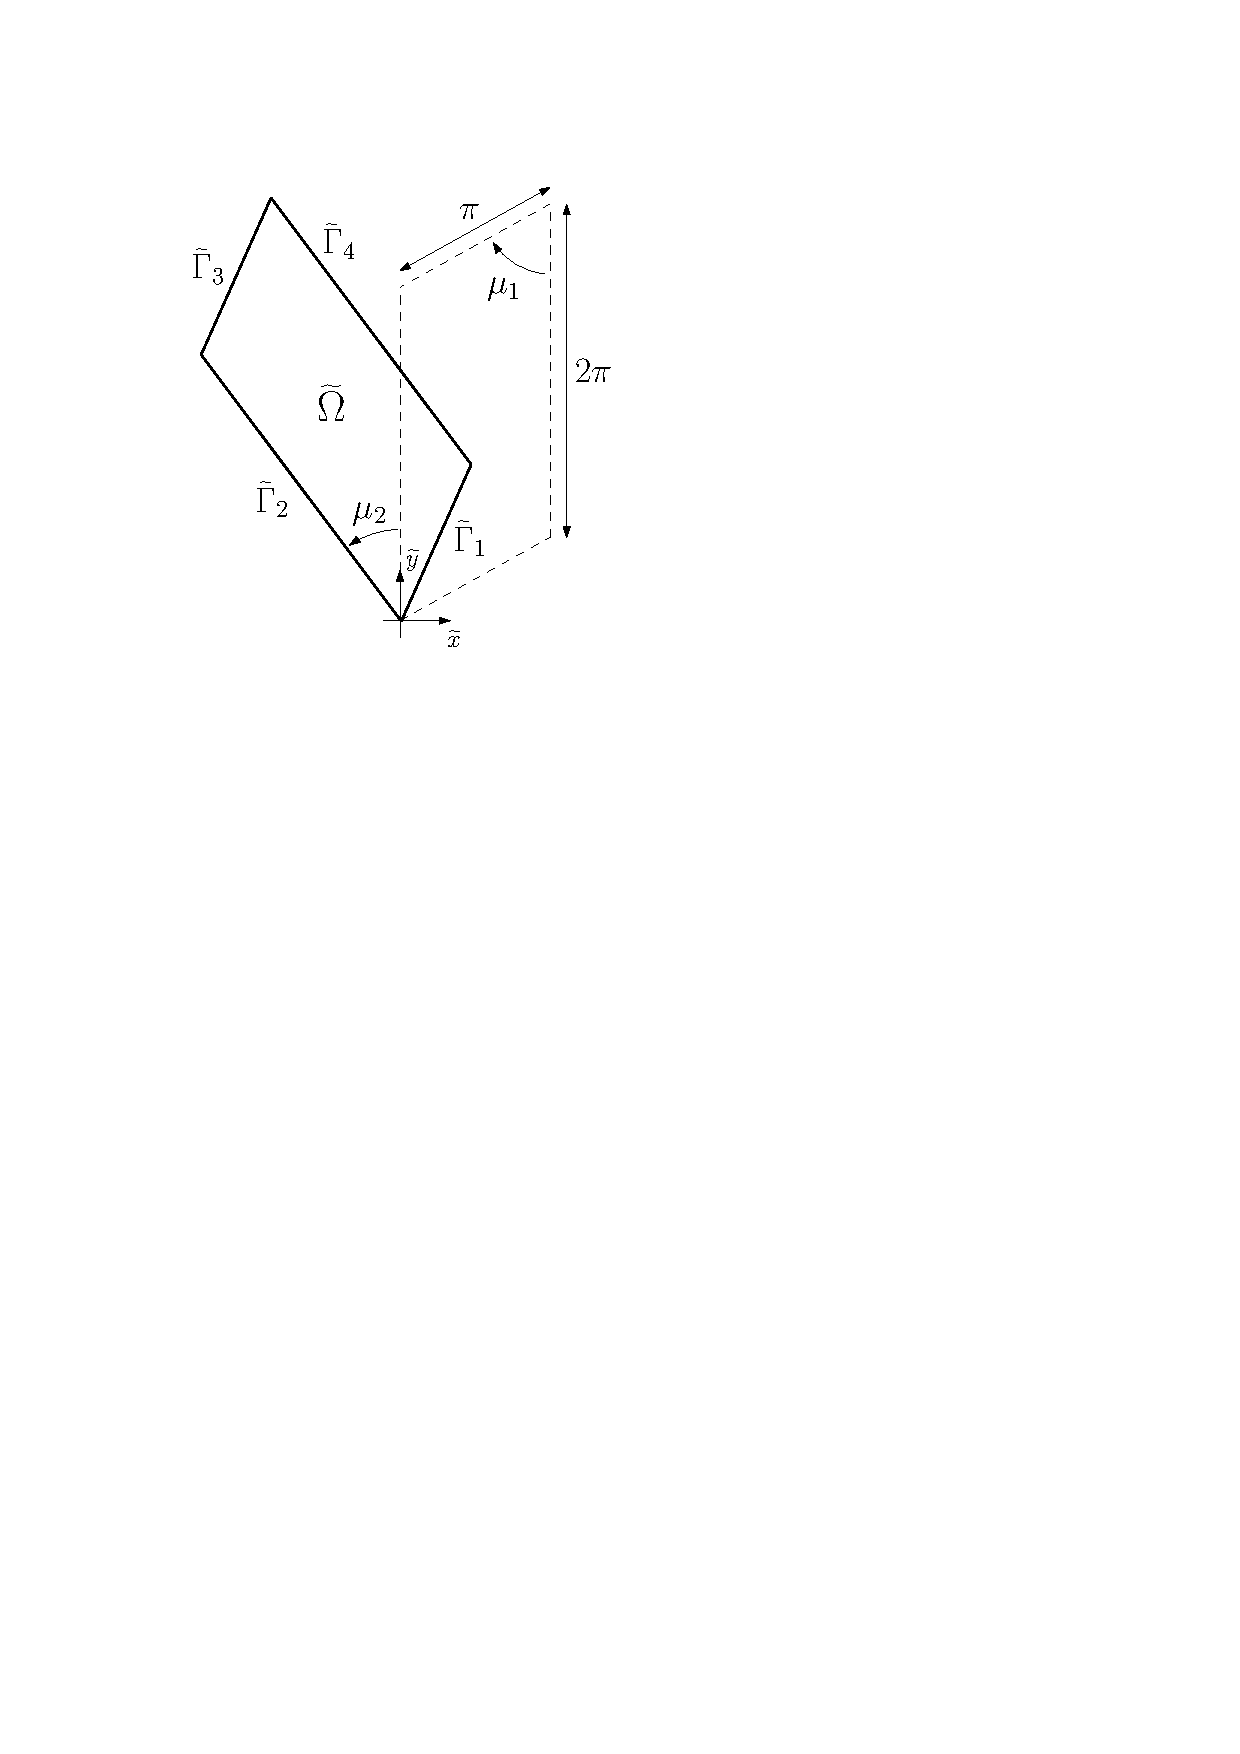
\includegraphics[scale = 0.65]{domain_square}
			
			\caption{The parametrized computational domain (solid line) for the Poisson problem \eqref{eq:nonlinear-poisson-example}.}
			\label{fig:nonlinear-poisson-example-domain}
		\end{figure}
		
		%\vspace*{0.5cm}
		
		\begin{figure}[H]
			\center
			\vspace*{-0.4cm}
			\subfloat{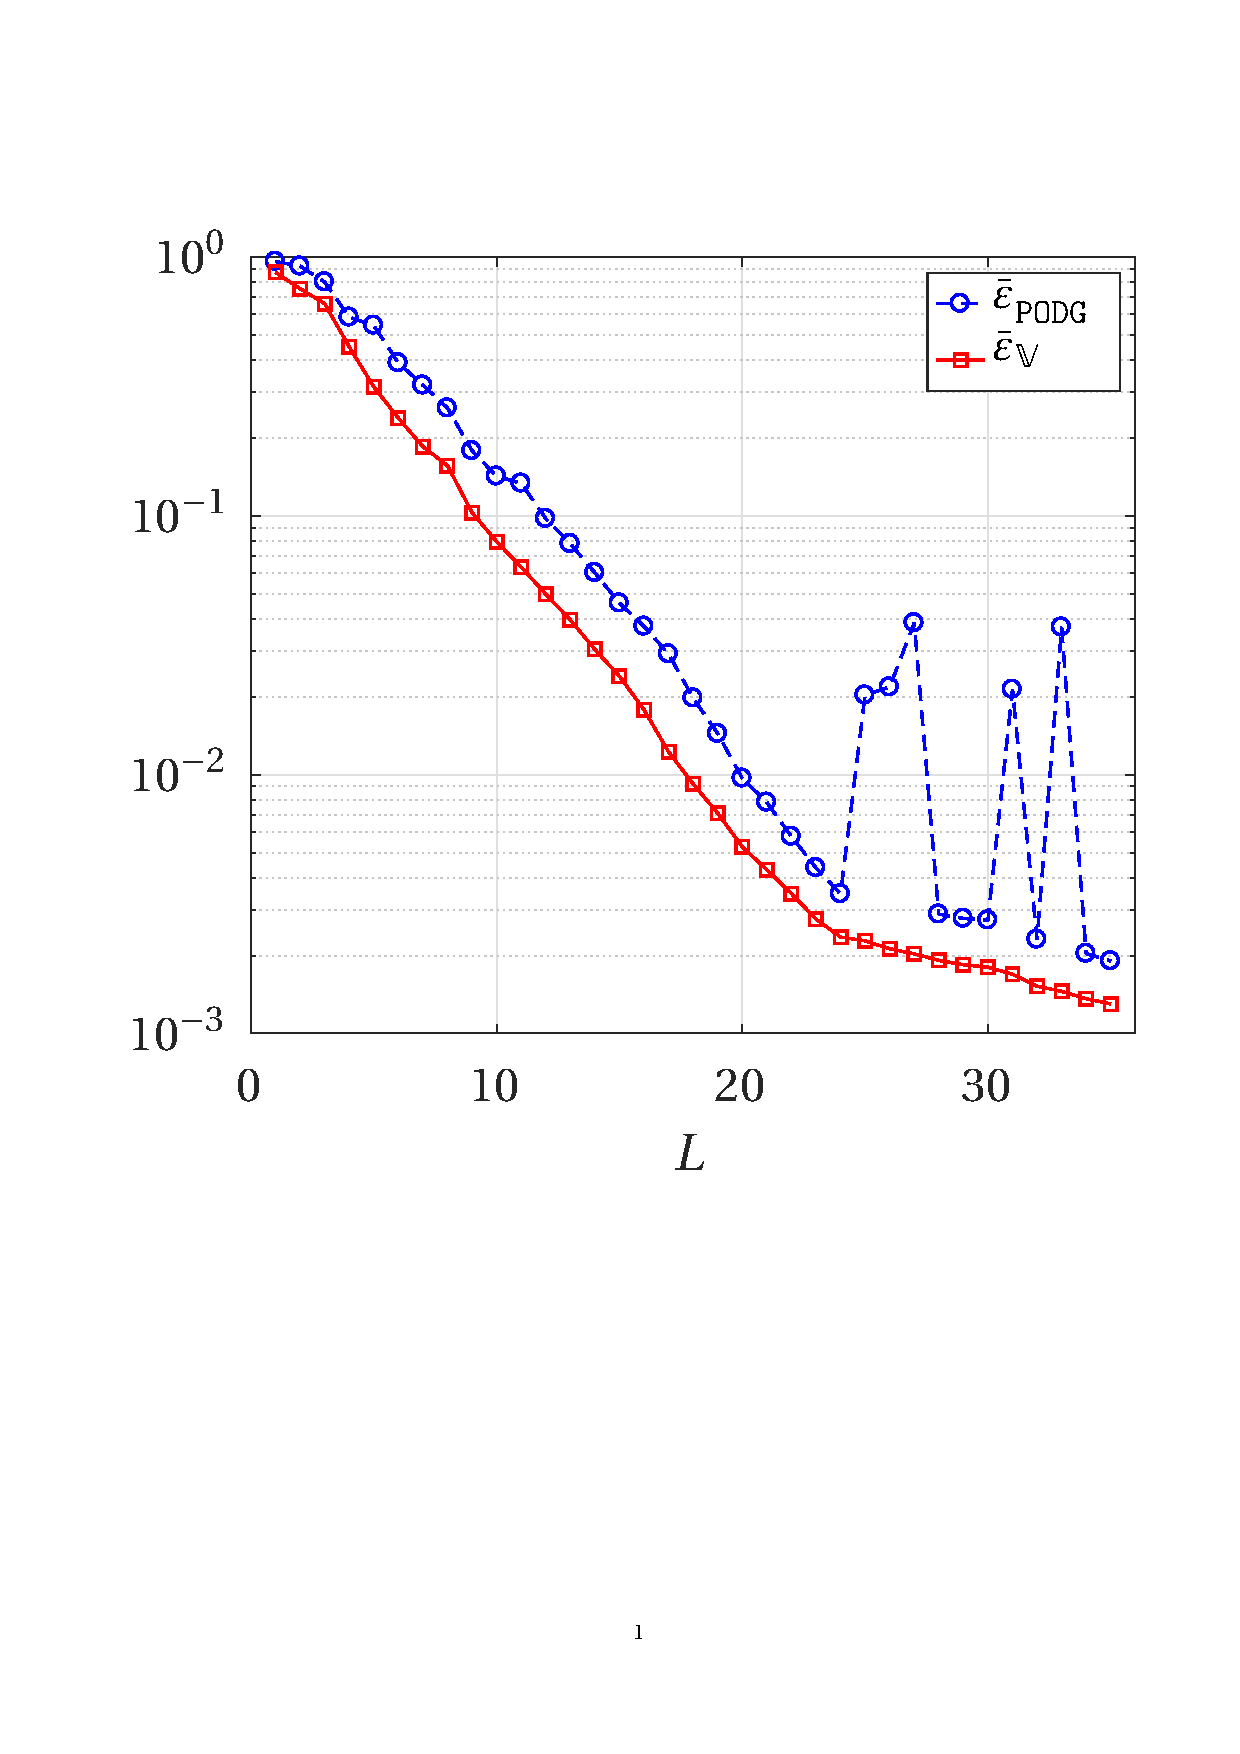
\includegraphics[scale = 0.40, trim = {1.5cm 9cm 1cm 3.75cm}, clip]{poisson2d_2_error_vs_rank_partial}}
			\hfill
			\subfloat{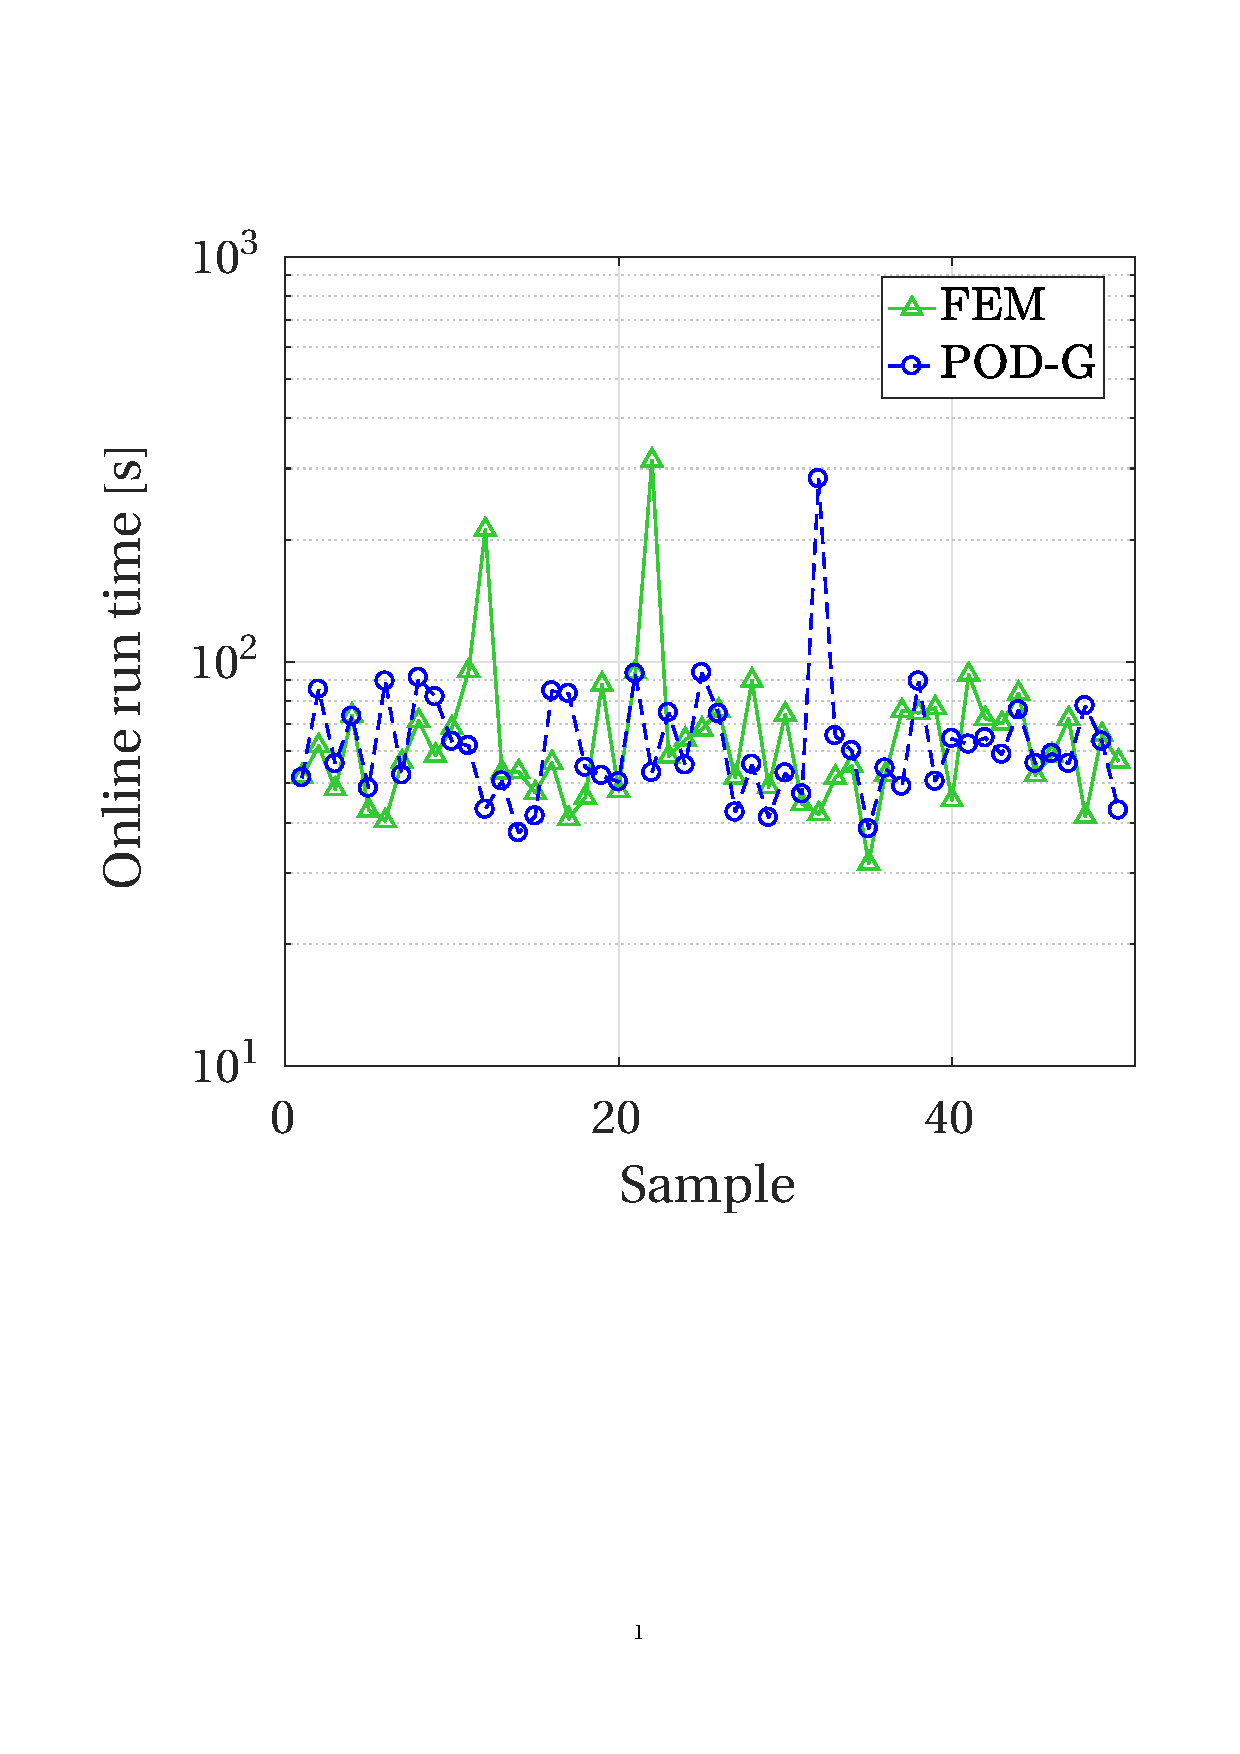
\includegraphics[scale = 0.40, trim = {1.5cm 9cm 1cm 3.75cm}, clip]{poisson2d_2_time_partial}}
						
			\caption{Left: average relative error between the FE solution for problem \eqref{eq:nonlinear-poisson-example} and either its projection onto the reduced space (red squares) or the POD-Galerkin RB solution (blue circles); the errors have been evaluated on a test parameter set $\Xi_{te} \subset \mathcal{P}$ consisting of $N_{te} = 50$ randomly picked values. Right: comparison between the online run times for the FE scheme and the POD-Galerkin method on $\Xi_{te}$, with $L = 35$ basis functions included in the reduced model.}
			\label{fig:nonlinear-poisson-example}
		\end{figure}
		
		\noindent Motivated by this last equality, once a reduced basis has been constructed (e.g., via POD of the snapshot matrix), we aim at approximating the function
		\begin{equation}
			\label{eq:map-to-approximate}
			\begin{aligned}
				\bg{\pi} ~ : ~ \mathcal{P} \subset \mathbb{R}^P ~ & \rightarrow ~ \mathbb{R}^L \\
				\bg{\mu} ~ & \mapsto ~ \mathbb{V}^T \mathbf{u}_h(\bg{\mu}) \, ,
			\end{aligned}
		\end{equation}
		mapping each input vector parameter $\bg{\mu} \in \mathcal{P}$ to the coefficients $\mathbb{V}^T \mathbf{u}_h(\bg{\mu})$ for the expansion of $u^{\mathbb{V}}_h$ in the reduced basis $\big\lbrace \psi_i \big\rbrace_{i = 1}^L$. Then, given a new parameter instance $\bg{\mu}$, the associated RB solution is simply given by the evaluation in $\bg{\mu}$ of the approximation $\hat{\bg{\pi}}$ of $\bg{\pi}$, i.e.
		\begin{equation*}
			\mathbf{u}_{\texttt{rb}}(\bg{\mu}) = \hat{\bg{\pi}}(\bg{\mu}) \, ,
		\end{equation*}
		and, consequently,
		\begin{equation*}
			\mathbf{u}_L(\bg{\mu}) = \mathbb{V} ~ \hat{\bg{\pi}}(\bg{\mu}) \, .
		\end{equation*}
		It is worth pointing out that, provided that the construction of $\hat{\bg{\pi}}$ is entirely carried out within the offline stage, this approach leads to a \emph{non-intrusive} RB method, enabling a complete decoupling between the online step and the underlying full-order model. Moreover, the accuracy of the resulting reduced solution uniquely relies on the quality of the reduced basis and the effectiveness of the approximation $\hat{\bg{\pi}}$ of the map $\bg{\pi}$; we shall appreciate the consequence of these facts in the next section.
		
		In the literature, different approaches for the \emph{interpolation} of \eqref{eq:map-to-approximate} have been developed, e.g., exploiting some geometrical considerations concerning the solution manifold $\mathcal{M}$ \cite{Ams10}, or employing radial basis functions \cite{Chen17}. In this work we resort to neural networks, in particular multi-layer perceptrons, for the \emph{nonlinear regression} of the map $\bg{\pi}$, leading to the POD-NN RB method. As described in Chapter \ref{chapter:Introduction to neural networks}, any neural network is tailored for the particular application at hand by means of a preliminary \emph{training} phase. Here, we are concerned with a function regression task, thus we straightforwardly adopt a \emph{supervised learning} paradigm, training the perceptron via exposition to a collection of (known) input-output pairs
		\begin{equation*}
			P_{tr} = \big\lbrace \big( \bg{\mu}^{(i)}, \, \mathbb{V}^T \mathbf{u}_h \big( \bg{\mu}^{(i)} \big) \big) \big\rbrace_{i = 1}^{N_{tr}} \, .
		\end{equation*} 
		According to the notation and nomenclature introduced in the previous chapter, for $i = 1, \, \ldots \, , N_{tr}$, $\mathbf{p}_i = \bg{\mu}^{(i)} \in \mathbb{R}^P$ represents the \emph{input pattern} and $\mathbf{t}_i =  \mathbb{V}^T \mathbf{u}_h \big( \bg{\mu}^{(i)} \big) \in \mathbb{R}^L$ the associated \emph{teaching input}; together, they constitute a \emph{training pattern}. In this respect, note that the teaching inputs $\mathbb{V}^T \mathbf{u}_h \big( \bg{\mu}^{(i)} \big)$, $i = 1, \, \ldots \, , N_{tr}$, are generated through the FE solver. On the one hand, this ensures the reliability of the teaching patterns, given the assumed high-fidelity of the FE scheme (conversely to the reduced solver, as already appreciated before). On the other hand, this also suggests to incorporate the learning phase of the perceptron within the offline step of the POD-NN RB method, as described in Algorithm \ref{alg:pod-nn}. In doing so, we exploit the natural decoupling between the training and the evaluation of neural networks, thus fulfilling the necessary requirement to enable great online efficiency; we refer the reader to the following chapter for a numerical validation of this assertion. 
		
		However, let us point out that the design of an effective learning procedure may require a larger amount of snapshots than the generation of the reduced space does. Moreover, we discussed in Chapter \ref{chapter:Introduction to neural networks} the time-consuming yet unavoidable \emph{trial}-\emph{and}-\emph{error} approach which one should pursue in the search for an optimal network topology. To this end, we propose an automatic procedure, resumed in Algorithm \ref{alg:podnn-training}.
		
		While the Cybenko's theorems (see \ref{cybenko-first-rule} and \ref{cybenko-second-rule} in Section \ref{section:Network topologies}) allows us to consider perceptrons with no more than two hidden layers, no similar a priori and general results are available for the number $H$ of neurons per layer (to ease the work, we uniquely consider networks with the same number of neurons in both the first and the second hidden layer). Hence, given an initial amount $N_{tr}$ of training samples (say $N_{tr} = 100$), we train the network for increasing values of $H$, stopping when overfitting of training data occurs (due to an excessive number of neurons with respect to the number of training patterns). In case the best configuration, i.e., the one yielding the smallest error on a test data set, does not meet a desired level of accuracy, we generate a new set of snapshots, which will enlarge the current training set, and we then proceed to re-train the networks. At this point, it is worth pointing out two remarks. 
		\begin{enumerate}[label=(\roman*)]
			\vspace*{-0.1cm}
			\item We can now limit ourselves to network configurations including a number of neurons non-smaller than the current optimal network. Indeed, the error (on the test data set) yielded by a neural network is decreasing in the number of patterns it is exposed to during the learning phase, and the larger the number of neurons, the faster the decay.
			\vspace*{-0.7cm}
			\item In order to maximize the additional quantity of information available for the learning, we should ensure that the new training inputs, i.e., parameter values, do not overlap with the ones already present in the training parameter set. To this aim, we pursue an euristhic approach, employing, at each iteration, the latin hypercube sampling, which has proved to provide a good compromise between randomness and even covarage of the parameter domain; an example is offered in Fig. \ref{fig:lhs} for $\mathcal{P} \subset \mathbb{R}^2$.
		\end{enumerate} 
		\vspace*{-0.1cm}
		The procedure is then iterated until a satisfactory degree of accuracy and generalization is attained, or the maximum number of training patterns is reached. Therefore, the speed up enabled by the pursuit of a neural network-based approach to tackle any \emph{online} query comes at the cost of an extended \emph{offline} phase.
		
		\begin{algorithm}[H]	
			\begin{algorithmic}[1]
				\Function{$\left( \mathcal{N}^{opt}, \, \mathcal{V}^{opt}, \, \mathbf{w}^{opt} \right) = $ \\ \hspace*{0.5cm} PODNN\_training}{$\, \mathbb{V}$, $\varepsilon$, $N_{tr}^{max}$, $H^{max}$, $N_{te}$, $d$, $K_{ms}$, $\delta$, $T$, $K_{ea}$}
					\vspace*{0.2cm}
					\State set $\Delta N = 100$, ~ $H_0 = 5$, ~ $\Delta H = 5$, ~ $N_{va} = \lceil 0.3 N_{tr}^{max} \rceil$ \Comment{Adjustable parameters}
					\State randomly drawn validation and test samples $\Xi_{va} = \big\lbrace \bg{\mu}_{va}^{(i)} \big\rbrace_{i = 1}^{N_{va}}$ and $\Xi_{te} = \big\lbrace \bg{\mu}_{te}^{(i)} \big\rbrace_{i = 1}^{N_{te}}$
					\State compute $\big\lbrace \mathbf{u}_h \big( \bg{\mu}_{va}^{(i)} \big) \big\rbrace_{i = 1}^{N_{va}}$ and $\big\lbrace \mathbf{u}_h \big( \bg{\mu}_{te}^{(i)} \big) \big\rbrace_{i = 1}^{N_{te}}$
					\State set $P_{va} = \big\lbrace \big( \bg{\mu}_{va}^{(i)}, \, \mathbb{V}^T \mathbf{u}_h \big( \bg{\mu}_{va}^{(i)} \big) \big) \big\rbrace_{i = 1}^{N_{va}}$ and $P_{te} = \big\lbrace \big( \bg{\mu}_{te}^{(i)}, \, \mathbb{V}^T \mathbf{u}_h \big( \bg{\mu}_{te}^{(i)} \big) \big) \big\rbrace_{i = 1}^{N_{te}}$
					\State evaluate projection error $E_{\texttt{POD}} = \nicefrac{1}{N_{te}} \sum_{i = 1}^{N_{te}} \norm{\mathbf{u}_h \big( \bg{\mu}_{te}^{(i)} \big) - \mathbb{V} \, \mathbb{V}^T \mathbf{u}_h \big( \bg{\mu}_{te}^{(i)} \big)}$
					\State $P_{tr} = \emptyset$, $N_{tr} = 0$, $H^{opt} = H_0$
					\DoWhile
						\State $N_{tr} \leftarrow N_{tr} + \Delta N$
						\State generate training samples $\Xi_{tr} = \big\lbrace \bg{\mu}_{tr}^{(i)} \big\rbrace_{i = 1}^{N_{tr}}$ via Latin Hypercube Sampling (LHS)
						\State compute snapshots $\big\lbrace \mathbf{u}_h \big( \bg{\mu}_{tr}^{(i)} \big) \big\rbrace_{i = 1}^{N_{tr}}$
						\State extend training data set: $P_{tr} \leftarrow P_{tr} \cup \big\lbrace \big( \bg{\mu}_{tr}^{(i)}, \, \mathbb{V}^T \mathbf{u}_h \big( \bg{\mu}_{tr}^{(i)} \big) \big) \big\rbrace_{i = 1}^{N_{tr}}$
						\State $E_{\texttt{NN}}^{opt} = \infty$, $H = H^{opt}$
						\While{$H \leq H^{max}$ and $E_{te} < E_{te}^{old}$}
							\State design a three-layers perceptron $\big( \mathcal{N}, \, \mathcal{V} \big)$ with $H$ neurons per hidden layer
							\State $\big[ \mathbf{w}, \, E_{\texttt{NN}} \big] = $ \Call{Training}{$\left( \mathcal{N}, \, \mathcal{V} \right)$, $P_{tr}$, $P_{va}$, $P_{te}$, $d$, $K_{ms}$, $\delta$, $T$, $K_{ea}$}
							\If{$E_{\texttt{NN}} < E_{\texttt{NN}}^{opt}$}
								\State $E_{\texttt{NN}}^{opt} = E_{\texttt{NN}}$, ~ $\mathcal{N}^{opt} = \mathcal{N}$, ~ $\mathcal{V}^{opt} = \mathcal{V}$, ~ $\mathbf{w}^{opt} = \mathbf{w}$, ~ $H^{opt} = H$
								\State $H \leftarrow H + \Delta H$
							\Else \Comment{Too many neurons: the network overfits training data}
								\State \textbf{break}
							\EndIf
						\EndWhile
					\EndDoWhile{$N_{tr} \leq N_{tr}^{max}$ and $\abs{E_{\texttt{POD}} - E_{\texttt{NN}}^{opt}} > \varepsilon$}
				\EndFunction
				
			\end{algorithmic}
			
			\caption{Selection of an optimal network configuration.}
			\label{alg:podnn-training}
		\end{algorithm}
								
		\noindent As described in Section \ref{section:Levenberg-Marquardt algorithm}, in our numerical tests we resort to the Levenberg-Marquardt algorithm to properly adjust the weights of the perceptron during the learning phase, relying on the Mean Squared Error (MSE) \eqref{eq:mse} as performance function. To motivate this choice, let 
		\begin{equation*}
			\mathbf{u}_{\texttt{rb}}^{\texttt{NN}}(\bg{\mu}) \in \mathbb{R}^L
		\end{equation*}
		be the (actual) output provided by the network for a given input $\bg{\mu}$, and 
		\begin{equation*}
			\mathbf{u}_L^{\texttt{NN}}(\bg{\mu}) = \mathbb{V} ~ \mathbf{u}_{\texttt{rb}}^{\texttt{NN}}(\bg{\mu}) \in \text{Col}(\mathbb{V}) \subset \mathbb{R}^M \, . 
		\end{equation*}
		Then (omitting the dependence on the input vector to ease the notation):
		\begin{equation}
			\label{eq:pod-nn-mse}
			\begin{aligned}
				MSE \big( \mathbf{u}_{\texttt{rb}}^{\texttt{NN}}, \, \mathbb{V}^T \mathbf{u}_h \big) & \propto \norm{\mathbf{u}_{\texttt{rb}}^{\texttt{NN}} - \mathbb{V}^T \mathbf{u}_h}^2_{\mathbb{R}^L} = \big( \mathbf{u}_{\texttt{rb}}^{\texttt{NN}} - \mathbb{V}^T \mathbf{u}_h \big)^T \big( \mathbf{u}_{\texttt{rb}}^{\texttt{NN}} - \mathbb{V}^T \mathbf{u}_h \big) \\
				& = \big( \mathbf{u}_{\texttt{rb}}^{\texttt{NN}} - \mathbb{V}^T \mathbf{u}_h \big)^T \underbrace{\mathbb{V}^T \mathbb{V}}_{\mathbb{I}_L \in \mathbb{R}^{L \times L}} \big( \mathbf{u}_{\texttt{rb}}^{\texttt{NN}} - \mathbb{V}^T \mathbf{u}_h \big) \\
				& = \big( \mathbb{V} ~ \mathbf{u}_{\texttt{rb}}^{\texttt{NN}} - \mathbb{V} ~ \mathbb{V}^T \mathbf{u}_h \big)^T \big( \mathbb{V} ~ \mathbf{u}_{\texttt{rb}}^{\texttt{NN}} - \mathbb{V} ~ \mathbb{V}^T \mathbf{u}_h \big) \\
				& = \norm{\mathbf{u}_L^{\texttt{NN}} - \mathbb{V} ~ \mathbb{V}^T \mathbf{u}_h}^2_{\mathbb{R}^M} = \norm{u_L^{\texttt{NN}} - u_h^{\mathbb{V}}}^2_h \, ,
			\end{aligned}
		\end{equation} 
		where
		\begin{equation}
			\label{eq:pod-nn-solution}
			u_L^{\texttt{NN}}(\bg{x}; \, \bg{\mu}) = \sum_{i = 1}^L \big( \mathbf{u}_{\texttt{rb}}^{\texttt{NN}}(\bg{\mu}) \big)_i ~ \psi_i(\bg{x}) \in V_{\texttt{rb}} \, .
		\end{equation}
		Therefore, by minimizing the MSE, we actually minimize the distance (in the discrete norm $\norm{\cdot}_h$) between the approximation provided by the neural network and the projection of the FE solution onto the reduced space $V_{\texttt{rb}}$ for all the training inputs $\bg{\mu}^{(i)}$, $i = 1, \, \ldots \, , N_{tr}$. The proper \emph{generalization} to other parameter instances not included in the training set is then ensured by the implementation of suitable techniques (e.g., early stopping, generalized cross validation) aiming at preventing the network to \emph{overfit} the training data; see Section \ref{section:Practical considerations on the design of artificial neural networks} for further details.
		
		While we shall numerically show the actual effectiveness and efficiency of the POD-NN method in the upcoming chapter, in the following concluding section we aim at further investigating the accuracy which the proposed reduced basis strategy could provide. To this end, we develop a simplified \emph{a priori} error analysis. Yet, no rigorous proof is provided; rather, the goal is to give some insights on the potential of the method.
								
		\begin{figure}[H]
			\center
			\subfloat{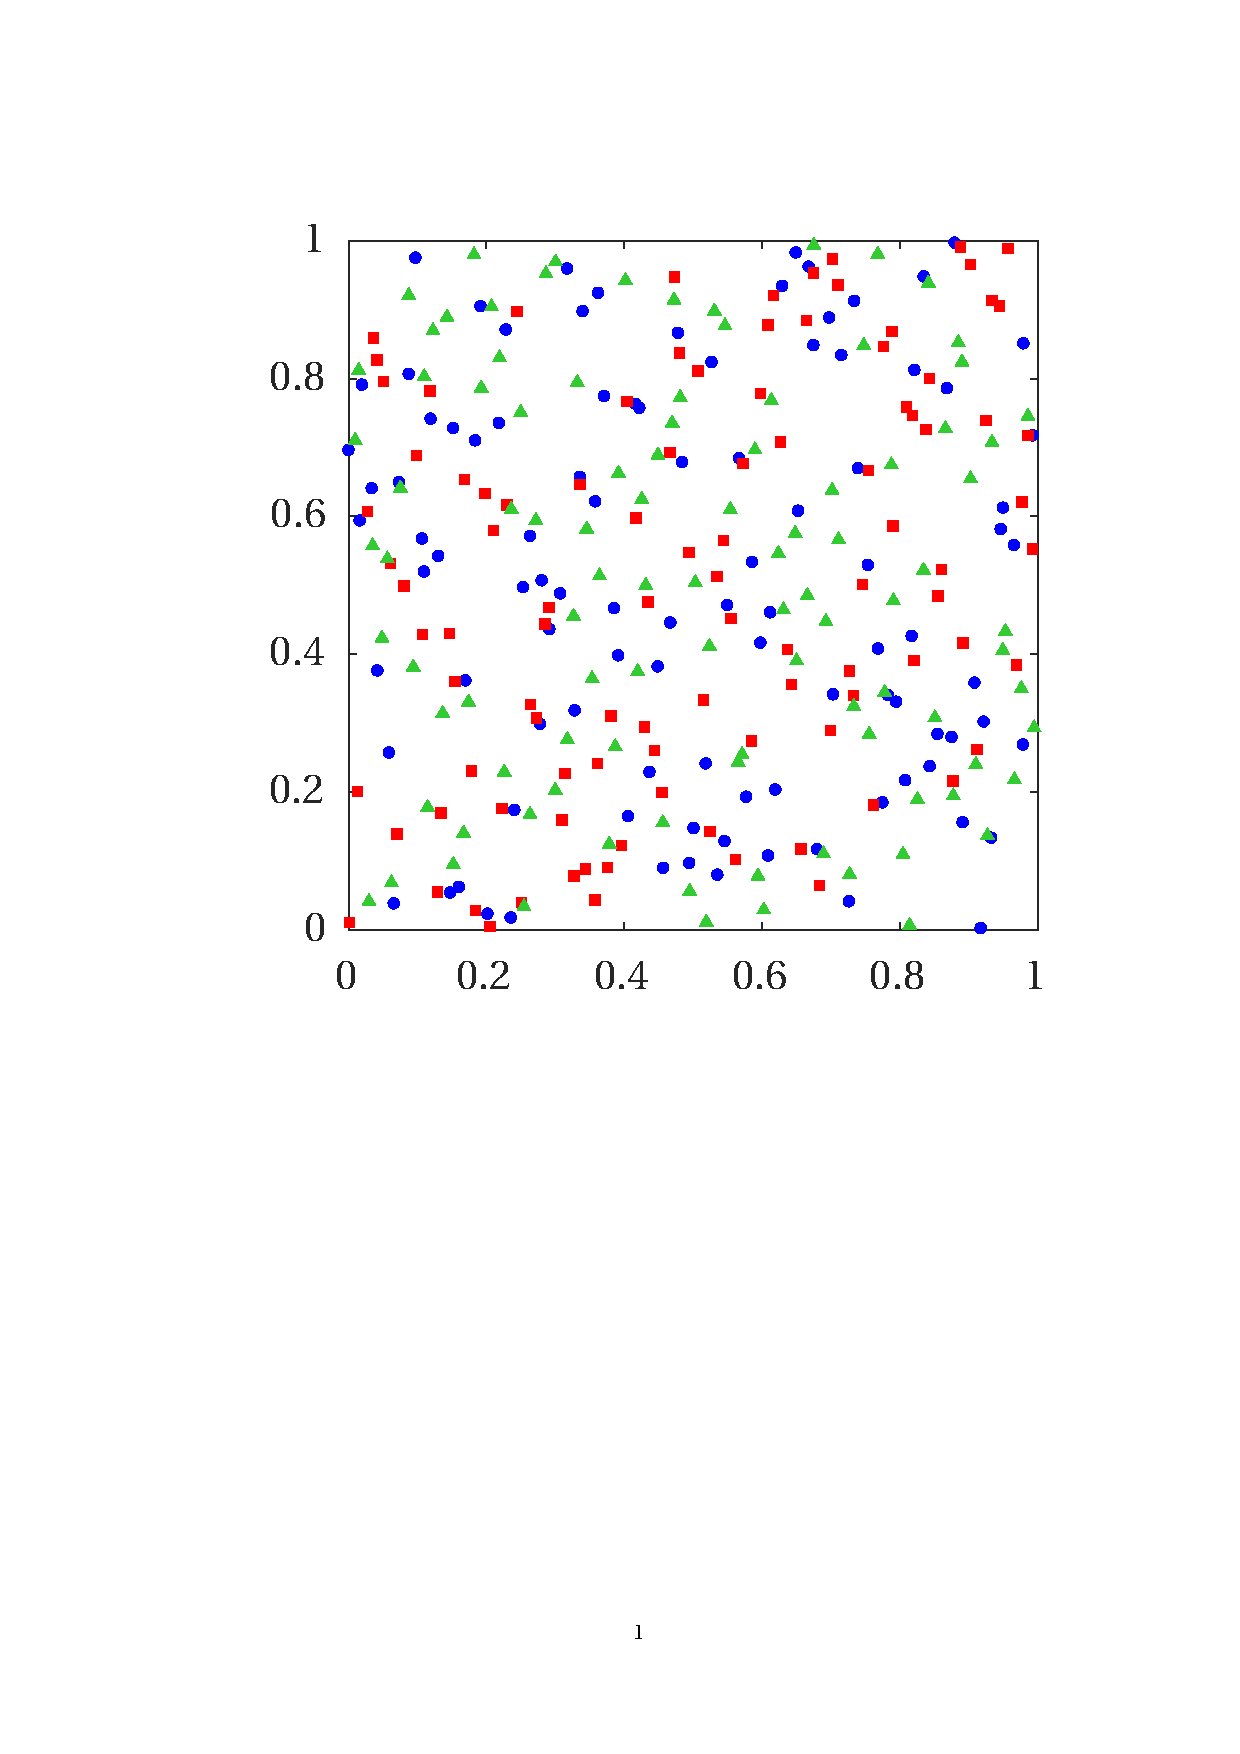
\includegraphics[scale = 0.475, trim = {1cm 12cm 2.5cm 3.5cm}, clip]{lhs_sample}}
			\subfloat{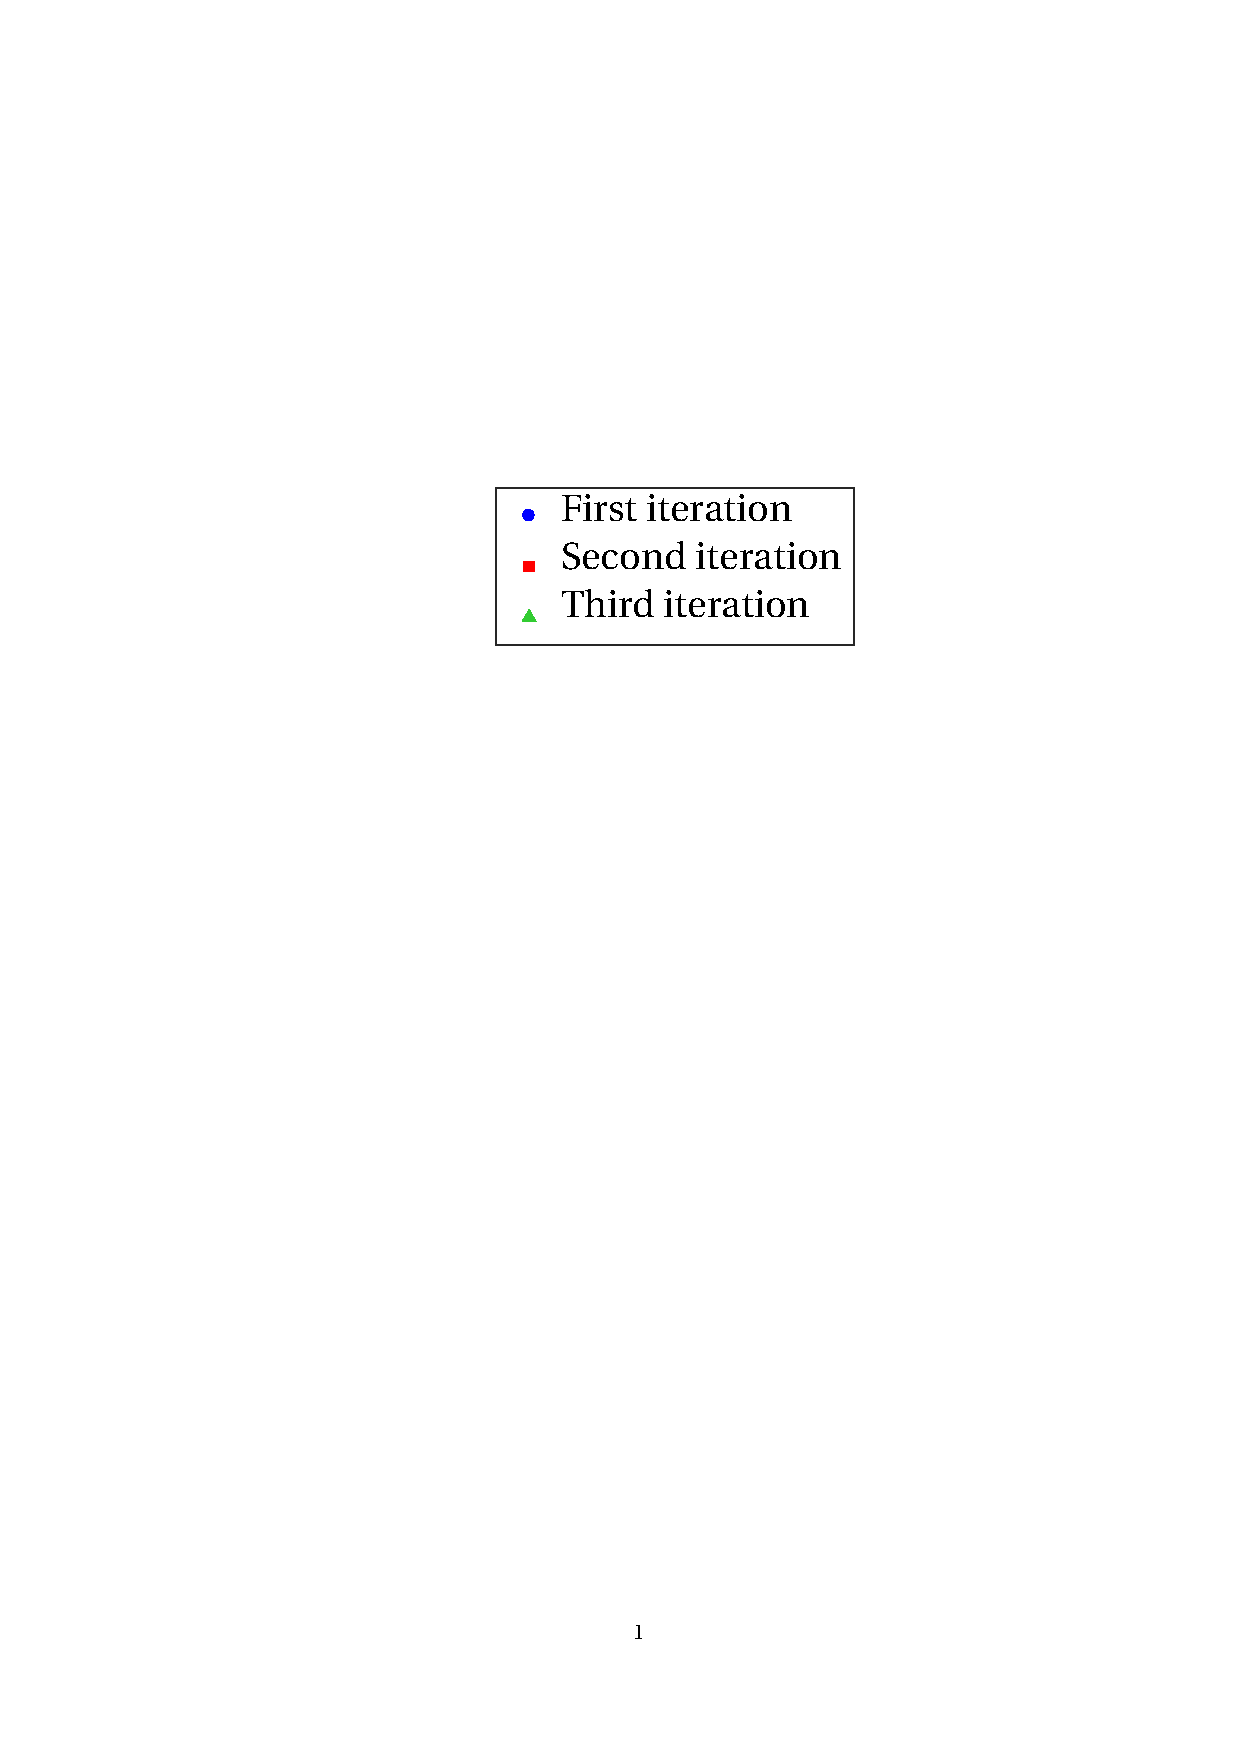
\includegraphics[scale = 0.55, trim = {8cm 13.4cm 1cm 8cm}, clip]{lhs_sample_legend}}
			
			\caption{Three point sets randomly generate through the latin hypercube sampling. Observe the good coverage provided by the union of the sets, with only a few overlapping points.}
			\label{fig:lhs}
		\end{figure}
		
		\algrenewcommand\textproc{}
		
		\begin{algorithm}[H]	
			\begin{algorithmic}[1]
				\Function{$\big[ \mathbb{V}, \mathcal{N}_{\texttt{rb}}, \mathcal{V}_{\texttt{rb}}, \bg{w}_{\texttt{rb}} \big] = $ \textsc{PODNN\_offline}}{$\mathcal{P}$, $\Omega_h$, $N$, $\delta_{\texttt{NWT}}$, $K_{max}$, $\delta_{\texttt{POD}}$, $\delta_{\texttt{NN}}$, $\varepsilon$, $N_{tr}^{max}$, $H^{max}$, $N_{te}$, $d$, $K_{ms}$, $T$, $K_{ea}$}
					\State solve the Laplace problems $\eqref{eq:laplace-problem-weight-function}$ and $\eqref{eq:laplace-problem-projection-function}$, yielding $\big\lbrace \xi_i \big\rbrace_{i = 1}^n$ and $\big\lbrace \pi_i \big\rbrace_{i = 1}^n$
					\State generate the parameter set $\Xi_N = \big\lbrace \bg{\mu}^{(1)}, \, \ldots \, , \bg{\mu}^{(N)} \big\rbrace$
					\State $\mathbf{u}_h \big( \bg{\mu}^{(i)} \big) = $ \Call{\textsc{Newton}}{$\bg{\mu}^{(i)}$, $\mathbf{u}_h^0$, $\big\lbrace \xi_i \big\rbrace_{i = 1}^n$, $\big\lbrace \pi_i \big\rbrace_{i = 1}^n$, $\delta_{\texttt{NWT}}$, $K_{max}$}, ~ for $i = 1, \, \ldots \, , N$
					\State $\mathbb{S} = \big[ \mathbf{u}_h \big( \bg{\mu}^{(1)} \big) \, \big| \, \ldots \, \big| \, \mathbf{u}_h \big( \bg{\mu}^{(N)} \big) \big]$
					\State $\mathbb{V} = $ \Call{\textsc{POD}}{$\mathbb{S}$, $\delta_{\texttt{POD}}$}
					\State $\big( \mathcal{N}_{\texttt{rb}}, \, \mathcal{V}_{\texttt{rb}}, \, \mathbf{w}_{\texttt{rb}} \big) = $ \Call{\textsc{PODNN\_training}}{$\, \mathbb{V}$, $\varepsilon$, $N_{tr}^{max}$, $H^{max}$, $N_{te}$, $d$, $K_{ms}$, $\delta_{\texttt{NN}}$, $T$, $K_{ea}$}
				\EndFunction
				
				\vspace*{0.3cm}
				
				\setcounter{ALG@line}{0}
				
				\Function{$\mathbf{u}_L^{\texttt{NN}} (\bg{\mu}) = $ \textsc{PODNN\_online}}{$\bg{\mu}$, $\mathbb{V}$, $\mathcal{N}_{\texttt{rb}}$, $\mathcal{V}_{\texttt{rb}}$, $\mathbf{w}_{\texttt{rb}}$}
					\State evaluate the output $\mathbf{u}_{\texttt{rb}}^{\texttt{NN}}(\bg{\mu})$ of the network $\big( \mathcal{N}_{\texttt{rb}}, \, \mathcal{V}_{\texttt{rb}}, \, \mathbf{w}_{\texttt{rb}} \big)$ for the input vector $\bg{\mu}$
					\State $\mathbf{u}_L^{\texttt{NN}} (\bg{\mu}) = \mathbb{V} \, \mathbf{u}_{\texttt{rb}}^{\texttt{NN}}(\bg{\mu})$
				\EndFunction
			\end{algorithmic}
			
			\caption{The offline and online stages for the POD-NN RB method.}
			\label{alg:pod-nn}
		\end{algorithm}
		
		\algrenewcommand\textproc{\textsc}
		
	\vspace*{0.01cm}
				
	\subsection{An a priori error analysis}
	\label{section:An a priori error analysis}
	
		For the sake of convenience, we directly consider the variational problem \eqref{eq:pde-weak-reference} stated over the reference domain $\Omega$. As usual, let $u(\bg{\mu}) \in V \subseteq H^1(\Omega)$ be the exact weak solution, $u_h(\bg{\mu}) \in V_h$ the high-fidelity discrete solution (obtained, e.g., through the finite element method) with $u_h^{\mathbb{V}}(\bg{\mu}) \in V_{\texttt{rb}}$ its projection onto $V_{\texttt{rb}}$, and $u_L^{\texttt{NN}}(\bg{\mu}) \in V_{\texttt{rb}}$ the reduced solution provided by the POD-NN method, defined in Eq. \eqref{eq:pod-nn-solution}. Omitting the dependence on the parameter $\bg{\mu}$, a straightforward application of the triangular inequality yields the following upper bound for the $L^2(\Omega)$-norm of the error committed by POD-NN RB method:
		\begin{equation}
			\label{eq:error-analysis-1}
			\norm{u - u_L^{\texttt{NN}}}_{L^2(\Omega)} \leq \norm{u - u_h}_{L^2(\Omega)} + \norm{u_h - u_h^{\mathbb{V}}}_{L^2(\Omega)} + \norm{u_h^{\mathbb{V}} - u_L^{\texttt{NN}}}_{L^2(\Omega)} \, .
		\end{equation}
		Let us analyze the three terms appearing on the right-hand side of \eqref{eq:error-analysis-1}. The former quantifies the discrepancy between the exact solution $u$ and the discrete approximation $u_h$ provided by the full-order solver. Throughout, we have assumed that $u_h$ can be driven as close as desired to $u$ in the $V$-norm; for instance, the FE solution can be improved either by refining the underlying mesh $\Omega_h$, or increasing the order of the interpolating polynomials, or both. Therefore:
		\begin{equation}
			\label{eq:error-analysis-2}
			\norm{u - u_h}_{L^2(\Omega)} \leq \norm{u - u_h}_V \leq \delta_{\texttt{HF}} \, ,
		\end{equation} 
		with $\delta_{\texttt{HF}} > 0$ being a given tolerance. Then, the term $\norm{u_h - u_h^{\mathbb{V}}}_{L^2(\Omega)}$ measures the distance between the truth solution and the reduced space $V_{\texttt{rb}}$. From the definitions \eqref{eq:galerkin-solution} and \eqref{eq:high-fidelity-projected}, it follows that:
		\begin{equation*}
			\begin{aligned}
				\norm{u_h - u_h^{\mathbb{V}}}_{L^2(\Omega)}^2 & = \int_{\Omega} \abs{u_h - u_h^{\mathbb{V}}}^2 \, d\Omega = \int_{\Omega} \abs{\sum_{i = 1}^M \big( \mathbf{u}_h \big)_i \phi_i - \sum_{i = 1}^M \big( \mathbb{V} \mathbb{V}^T \mathbf{u}_h \big)_i \phi_i}^2 \, d\Omega \\
				& = \sum_{i = 1}^M \sum_{j = 1}^M \big( \mathbf{u}_h - \mathbb{V} \mathbb{V}^T \mathbf{u}_h \big)_i \big( \mathbf{u}_h - \mathbb{V} \mathbb{V}^T \mathbf{u}_h \big)_j \underbrace{\int_{\Omega} \phi_i \, \phi_j \, d\Omega}_{\mathbb{M}_{i,j}} \\[-0.3cm]
				& = \big( \mathbf{u}_h - \mathbb{V} \mathbb{V}^T \mathbf{u}_h \big)^T \mathbb{M} \big( \mathbf{u}_h - \mathbb{V} \mathbb{V}^T \mathbf{u}_h \big) \, .
			\end{aligned}
		\end{equation*}
		where $\mathbb{M} \in \mathbb{R}^{M \times M}$ denotes the mass matrix. Exploiting the symmetry and positive definiteness of $\mathbb{M}$ (following from the symmetry and positiveness of the canonical scalar product $(\cdot,\cdot)_{L^2(\Omega)}$ of $L^2(\Omega)$), we further get:
		\begin{equation*}
			\norm{u_h - u_h^{\mathbb{V}}}_{L^2(\Omega)}^2 = \norm{\mathbb{M}^{1/2} \big( \mathbf{u}_h - \mathbb{V} \mathbb{V}^T \mathbf{u}_h \big)}^2_{\mathbb{R}^M} \leq \norm{\mathbb{M}}_2 \norm{\mathbf{u}_h - \mathbb{V} \mathbb{V}^T \mathbf{u}_h}_{\mathbb{R}^M}^2 \, ,
		\end{equation*}
		with $\norm{\cdot}_2$ the matrix $2$-norm. Suppose that all the parameters affecting the full-order solver (e.g., the grid size) are fixed, so that the mass matrix $\mathbb{M}$ keeps unchanged as the size $L$ of the reduced basis vary. Then, the error behaviour is entirely controlled by the term
		\begin{equation*}
			\norm{\mathbf{u}_h - \mathbb{V} \mathbb{V}^T \mathbf{u}_h}_{\mathbb{R}^M} \, ,
		\end{equation*}
		i.e., the distance (in the Euclidean norm) between $\mathbf{u}_h \in \mathbb{R}^M$ and its projection onto the column space $\text{Col}\mathbb{V}$ of $\mathbb{V}$. In this respect, let us recall that, at the algebraic level, the reduced basis vectors $\big\lbrace \bg{\psi}_i \big\rbrace_{i = 1}^L$ coincide with the first $L$ left singular vectors of the snapshot matrix $\mathbb{S} = \big[ \mathbf{u}_h\big( \bg{\mu}^{(1)} \big) \, \big| \, \ldots \, \big| \, \mathbf{u}_h\big( \bg{\mu}^{(N)} \big) \big] \in \mathbb{R}^{M \times N}$. From \eqref{eq:pod-error}, we already know that for the columns of $\mathbb{S}$, i.e., the vectors collecting the degrees of freedom for the snapshots, the following holds:
		\begin{equation*}
			\norm{\mathbf{u}_h\big(\bg{\mu}^{(n)}\big) - \mathbb{V} \mathbb{V}^T \mathbf{u}_h\big(\bg{\mu}^{(n)}\big)}_{\mathbb{R}^M}^2 = \sum_{j = L+1}^R \sigma_j^2 \, ,
		\end{equation*}
		with $R$ the rank of $\mathbb{S}$ and $\big\lbrace \sigma_j \big\rbrace_{j = 1}^R$ its singular values. The above estimate can be generalized without any further hypothesis and upon small modifications to all the other elements in the snapshot manifold $\mathcal{M}_{\Xi_N}$. To be extendible to the entire discrete solution manifold $\mathcal{M}_h$, we have to assume that $\mathcal{M}_h$ is a low-dimensional subspace of $V_h$, so that the ensemble of snapshots is actually representative of the entire $\mathcal{M}_h$. Then, further assuming a rapid (i.e., exponential) decay of the singular values with the order, we have
		\begin{equation}
			\label{eq:error-analysis-3}
			\norm{u_h - u_h^{\mathbb{V}}}_{L^2(\Omega)}^2 \approx \beta e^{-\alpha \, L} \, .
		\end{equation}
		The last term involved in \eqref{eq:error-analysis-1} regards the distance between $u_h^{\mathbb{V}}$ and $u_L^{\texttt{NN}}$, i.e. the POD-NN solution. Similar to what is done for the previous term, recalling the definition \eqref{eq:pod-nn-solution} for $u_L^{\texttt{NN}}$ we derive:
		\begin{equation}
			\label{eq:error-analysis-4}
			\begin{aligned}
				\norm{u_h^{\mathbb{V}} - u_L^{\texttt{NN}}}_{L^2(\Omega)} & = \int_{\Omega} \abs{u_h^{\mathbb{V}} - u_L^{\texttt{NN}}}^2 \, d\Omega = \int_{\Omega} \abs{\sum_{i = 1}^M \big( \mathbb{V} \mathbb{V}^T \mathbf{u}_h \big)_i \phi_i - \sum_{i = 1}^M \big( \mathbb{V} \mathbf{u}_{\texttt{rb}}^{\texttt{NN}} \big)_i \phi_i}^2 \, d\Omega \\
				& = \sum_{i = 1}^M \sum_{j = 1}^M \big( \mathbb{V} \mathbb{V}^T \mathbf{u}_h - \mathbb{V} \mathbf{u}_{\texttt{rb}}^{\texttt{NN}} \big)_i \big( \mathbb{V} \mathbb{V}^T \mathbf{u}_h - \mathbb{V} \mathbf{u}_{\texttt{rb}}^{\texttt{NN}} \big)_j \underbrace{\int_{\Omega} \phi_i \, \phi_j \, d\Omega}_{\mathbb{M}_{i,j}} \\[-0.4cm]
				& = \big( \mathbb{V} \mathbb{V}^T \mathbf{u}_h - \mathbb{V} \mathbf{u}_{\texttt{rb}}^{\texttt{NN}} \big)^T \mathbb{M} \big( \mathbb{V} \mathbb{V}^T \mathbf{u}_h - \mathbb{V} \mathbf{u}_{\texttt{rb}}^{\texttt{NN}} \big) \\
				& = \norm{\mathbb{M}^{1/2} \mathbb{V} \big( \mathbb{V}^T \mathbf{u}_h - \mathbf{u}_{\texttt{rb}}^{\texttt{NN}} \big)}_{\mathbb{R}^M}^2 \\
				& \leq \norm{\mathbb{M}}_2 \norm{\mathbb{V}}_2^2 \norm{\mathbb{V}^T \mathbf{u}_h - \mathbf{u}_{\texttt{rb}}^{\texttt{NN}}}_{\mathbb{R}^L}^2 \leq L \norm{\mathbb{M}}_2 \norm{\mathbb{V}^T \mathbf{u}_h - \mathbf{u}_{\texttt{rb}}^{\texttt{NN}}}_{\mathbb{R}^L}^2 \, ,
			\end{aligned}
		\end{equation}
		where the last inequality follows from
		\begin{equation*}
			\norm{\mathbb{V}}_2 \leq \norm{\mathbb{V}}_F = \sqrt{\text{tr} \big( \mathbb{V}^T \mathbb{V} \big)} = \sqrt{\text{tr} \big( \mathbb{I}_L \big)} = \sqrt{L} \, .
		\end{equation*}
		with $\norm{\cdot}_F$ the Frobenius norm and $\mathbb{I}_L \in \mathbb{R}^{L \times L}$ the identity matrix of dimension $L$. In \eqref{eq:error-analysis-4}, by \eqref{eq:pod-nn-mse} the term
		\begin{equation}
			\label{eq:error-analysis-5}
			\norm{\mathbb{V}^T \mathbf{u}_h - \mathbf{u}_L^{\texttt{NN}}}_{\mathbb{R}^L}
		\end{equation}
		coincides with the specific error function used to train the network. As for \eqref{eq:error-analysis-2}, this can be lowered to any given tolerance $\delta_{\texttt{NN}}$, thanks to the Cybenko's result (see \ref{cybenko-second-rule} in Section \ref{section:Network topologies}), which ensures that one can always design (and train) a three-layer perceptron which approximates the map \eqref{eq:map-to-approximate} to any desired level of accuracy, provided a sufficient number of training samples. However, as already pointed out in Section \ref{section:Practical considerations on the design of artificial neural networks}, no estimates on the convergence rate with respect to either the number of computing neurons or the dimension of the training set are available. Indeed, this is really problem dependent. Anyway, we shall see in the upcoming chapter that there exist some convenient situations in which the decay is surprisingly rapid. In this respect, let us notice that the factor $\sqrt{L}$ appearing in \eqref{eq:error-analysis-5} suggests that the attaining of the desired accuracy gets harder as the number of POD modes, i.e., the dimension of the output space $\mathbb{R}^L$, increases.
		
		Lastly, inserting \eqref{eq:error-analysis-2}, \eqref{eq:error-analysis-3} and \eqref{eq:error-analysis-4} into \eqref{eq:error-analysis-1}, we obtain the following estimate for the POD-NN error in the $L^2(\Omega)$-norm:
		\begin{equation*}
			\label{eq:error-analysis-final}
			\norm{u - u_L^{\texttt{NN}}}_{L^2(\Omega)} \leq \delta_{\texttt{HF}} + \beta e^{-\alpha \, L} + \gamma \sqrt{L} \, \delta_{\texttt{NN}} \, ,
		\end{equation*}
		with $\alpha$, $\beta$ and $\gamma$ positive constants, independent of both the solution and the size of the reduced basis, and $\delta_{\texttt{HF}}$ and $\delta_{\texttt{NN}}$ given tolerances. In other terms, the accuracy ensured by the POD-NN reduced basis method entirely relies on the accuracy of the underlying full-order solver, the quality of the reduced basis, and the accuracy of the approximation of the map \eqref{eq:map-to-approximate}.
				
	
		
	\chapter{Numerical results}
	\label{chapter:Numerical results}
	
		In this chapter, we present different numerical results obtained via the POD-G and the POD-NN reduced basis (RB) methods applied to parametrized full-Dirichlet boundary value problems (BVPs) for the (nonlinear) Poisson equation and the incompressible steady Navier-Stokes equations. The problems which shall be treated involve from $1$ up to $3$ parameters, either physical or geometrical. For the Poisson equation, we consider both linear and nonlinear problems, stated on either one- or two-dimensional domains. In the one-dimensional case, we deal uniquely with physical parameters, which address the diffusion coefficient, the source term or the boundary conditions; whereas in two spatial dimensions we let the parameters affect the shape of the domain, not the state equation. This latter remark also holds for the test cases concerning the Navier-Stokes equations. Particularly, we shall tackle the well-known lid-driven cavity problem for different values of the Reynold's number. The application of both the POD-G and the POD-NN techniques to differential problems featuring both physical and geometrical parameters, as well as natural or periodic boundary conditions, is left as future work.
		
		The two RB methodologies considered in this work are compared both in terms of accuracy and performance provided at the online stage. To this end, let $\mathbf{u}_L(\bg{\mu})$ and $\mathbf{u}_L^{\texttt{NN}}(\bg{\mu})$ be respectively the (algebraic) POD-G and POD-NN solutions of reduced order $L$ to the general $\bg{\mu}$-dependent problem $\eqref{eq:pde-weak-reference}$. Furthermore, let $\norm{\cdot}$ be the canonical (Euclidean) norm on $\mathbb{R}^M$. Once the offline phases for both the POD-G and the POD-NN method have been carried out, given a new parameter value $\bg{\mu} \in \mathcal{P}$ (not involved either in the generation of the POD basis nor in the detection of an optimal neural network) the following \emph{relative} errors with respect to the high-fidelity (finite element) solution $\mathbf{u}_h(\bg{\mu})$ are analyzed:
		\begin{enumerate}[label=(\alph*)]
			\item the POD-G relative error, that is
			\begin{equation}
				\label{eq:podg-error}
				\varepsilon_{\texttt{PODG}}^{}(L, \bg{\mu}) = \dfrac{\norm{\mathbf{u}_h(\bg{\mu}) - \mathbf{u}_L(\bg{\mu})}}{\norm{\mathbf{u}_h(\bg{\mu})}} = \dfrac{\norm{\mathbf{u}_h(\bg{\mu}) - \mathbb{V} \, \mathbf{u}_{\texttt{rb}}(\bg{\mu})}}{\norm{\mathbf{u}_h(\bg{\mu})}} \, ;
			\end{equation} 
			\item the POD-NN relative error, that is
			\begin{equation}
				\label{eq:podnn-error}
				\varepsilon_{\texttt{PODNN}}^{}(L, \bg{\mu}) = \dfrac{\norm{\mathbf{u}_h(\bg{\mu}) - \mathbf{u}_L^{\texttt{NN}}(\bg{\mu})}}{\norm{\mathbf{u}_h(\bg{\mu})}} = \dfrac{\norm{\mathbf{u}_h(\bg{\mu}) - \mathbb{V} \, \mathbf{u}_{\texttt{rb}}^{\texttt{NN}}(\bg{\mu})}}{\norm{\mathbf{u}_h(\bg{\mu})}} \, ;
			\end{equation} 
			\item the relative projection error, i.e., the error committed by approximating the high-fidelity solution with its projection (in the discrete scalar product $(\cdot,\cdot)_h$, see Eq. \eqref{eq:discrete-scalar-product}) onto the reduced space $V_{\texttt{rb}}$, namely
			\begin{equation}
				\label{eq:projection-error}
				\varepsilon_{\mathbb{V}}^{}(L, \bg{\mu}) = \dfrac{\norm{\mathbf{u}_h(\bg{\mu}) - \mathbf{u}_h^{\mathbb{V}}(\bg{\mu})}}{\norm{\mathbf{u}_h(\bg{\mu})}} = \dfrac{\norm{\mathbf{u}_h(\bg{\mu}) - \mathbb{V} \mathbb{V}^T \mathbf{u}_h(\bg{\mu})}}{\norm{\mathbf{u}_h(\bg{\mu})}} \, ;
			\end{equation}
			recall that \eqref{eq:projection-error} provides a lower-bound for both \eqref{eq:podg-error} and \eqref{eq:podnn-error}. 
		\end{enumerate}
		The above errors are then evaluated on a test parameter set $\Xi_{te} \subset \mathcal{P}$ consisting of $N_{te}$ randomly picked samples. Upon choosing a sufficiently large number of test values, statistics for $\varepsilon_{\texttt{PODG}}^{}(L, \cdot)$, $\varepsilon_{\texttt{PODNN}}^{}(L, \cdot)$ and $\varepsilon_{\mathbb{V}}^{}(L, \cdot)$ on $\Xi_{te}$ can be reasonably assumed independent of the particular choice made for $\Xi_{te}$, thus making any subsequent error analysis reliable. In particular, in our numerical studies we let $N_{te}$ range from $50$ up to $100$, and we consider the average of the errors over the test data set, respectively denoted by
		\begin{equation*}
			\text{$\bar{\varepsilon}_{\texttt{PODG}}^{} = \bar{\varepsilon}_{\texttt{PODG}}^{}(L)$, \hspace*{0.2cm} $\bar{\varepsilon}_{\texttt{PODNN}}^{} = \bar{\varepsilon}_{\texttt{PODNN}}^{}(L)$ \hspace*{0.2cm} and \hspace*{0.2cm} $\bar{\varepsilon}_{\mathbb{V}}^{} = \bar{\varepsilon}_{\mathbb{V}}^{}(L)$ \, .}
		\end{equation*} 
		Before diving into the results, let us give some details on the training phase for neural networks. While the training samples $\Xi_{tr} \subset \mathcal{P}$ are generated via successive latin hypercube samplings (as described in Algorithm \ref{alg:podnn-training}), the validation inputs $\Xi_{va} \subset \mathcal{P}$ are randomly picked through a Monte Carlo sampling, as done for $\Xi_{te}$. The ratio between the size of $\Xi_{va}$ and $\Xi_{tr}$ is set to $0.3$. The training is then performed by resorting to the multiple restarts approach to prevent the results to depend on the way the weights are (randomly) initialized (see Section \ref{section:Practical considerations on the design of artificial neural networks}). Typically, $K_{ms} = 5$ restarts for each network topology are performed. To ease the search for an optimal network configuration, by exploiting Cybenko's results (see \ref{cybenko-first-rule} and \ref{cybenko-second-rule} in Section \ref{section:Network topologies}) we limit ourselves to two- and three-layers neural networks; in the latter case, we consider the same number of neurons for both hidden layers. For each topology, the hyperbolic tangent (see Fig. \ref{fig:activation-functions}, on the right) is used as activation function for the hidden (computing) neurons.  
		
		A last relevant remark concerns the choice of the number of POD modes $L$ to be retained in the model. To this end, in a production framework one could employ, e.g., the relative information content criterium \eqref{eq:relative-information-content}. Here, for the sake of analysis, we pursue a different approach, evaluating the errors \eqref{eq:podg-error}, \eqref{eq:podnn-error} and \eqref{eq:projection-error} (averaged over $\Xi_{te}$) for some (and often all) $L \leq L_{max}$ (say $L_{max} = 40$). In this respect, we point out that within the POD-NN framework, once a neural network has been (properly) trained for the approximation of the vectored-value map \eqref{eq:map-to-approximate} with $L$ components, then the approximation of the very same map for any $\bar{L} < L$ comes freely by simply retaining the first $\bar{L}$ entries of the network output vector. Therefore, no additional training is required. Indeed, decorating the matrix $\mathbb{V}$ with a superscript denoting the dimension of the represented basis, one has
		\begin{equation*}
			\mathbb{V}^{l+1} = \big[ \underbrace{\bg{\psi}_1 \, \big| \, \ldots \, \big| \, \bg{\psi}_l}_{\mathbb{V}^l} \, \big| \, \bg{\psi}_{l+1} \big] = \big[ \mathbb{V}^l \, \big| \, \bg{\psi}_{l+1} \big] \hspace*{0.3cm} \text{for any $l < M$} \, .
		\end{equation*}
		Conversely, we have already appreciated in Section \ref{section:A POD-based RB method using neural networks} how the convergence provided by Newton's method may depend on the size $L$ of the reduced basis. Therefore, for a fair comparison with the POD-NN method we shall explicitly assemble and solve the reduced system for any $\bg{\mu} \in \Xi_{te}$ and any tested value of $L$.
			
	\section{One-dimensional Poisson equation}
	\label{section:One-dimensional Poisson equation (results)}
	
		As a preliminar step before tackling more probing problems in two spatial dimensions, in this section we consider BVPs for the one-dimensional Poisson equation. Three test cases are examined: the first linear and the others nonlinear, involving an increasing number of parameters. 
		
	\vspace*{0.3cm}
	
	\subsection{Linear test case}
	\label{section:poisson1d-1}
	
		We first consider the following linear Poisson equation in $\Omega = (-1,1)$:
		\begin{equation}
			\label{eq:poisson1d-1}
			- u(\mu)'' = \dfrac{1}{\sqrt{2 \pi \sigma^2}} \exp \left( -\dfrac{\mu}{2 \sigma^2} \right) \, ,
		\end{equation}
		with $\sigma = 0.2$ (fixed) and $\mu \in [-1,1]$. The equation is completed with homogeneous Dirichlet boundary conditions. In order to derive a POD-Galerkin reduced basis model for \eqref{eq:poisson1d-1}, we first generate a collection of linear finite elements discretizations $\big\lbrace \mathbf{u}_h \big( \mu^{(1)} \big), \, \ldots \, , \mathbf{u}_h \big( \mu^{(N)} \big) \big\rbrace$ over a (physical) uniform grid with $100$ points. Here, the latin hypercube sampling is not usable, since the parameter domain $\mathcal{P} \equiv [-1,1]$ is one-dimensional, whereas we displace the training samples $\big\lbrace \mu^{(1)}, \, \ldots \, , \mu^{(N)} \big\rbrace$ uniformly over $\mathcal{P}$. In the left plot of Fig. \ref{fig:poisson1d-1-fig1}, we analyze the relative error between the FE and the POD-Galerkin solutions. The error is averaged over an ensemble $\Xi_{te}$ of $N_{te} = 100$ parameter values. Independently of the number of snapshots used to generate the POD basis, we can appreciate an exponential decay of the error with the number $L$ of POD modes retained by the reduced model, coherently with the behaviour exhibited by the singular values. The effectiveness of the RB approximation is confirmed by the second plot of Fig. \ref{fig:poisson1d-1-fig1}, showing the FE and the POD-G solutions for three values of $\mu$, with $N = 50$ and $L = 10$.
		
		\begin{figure}[H]
			\center
			\subfloat{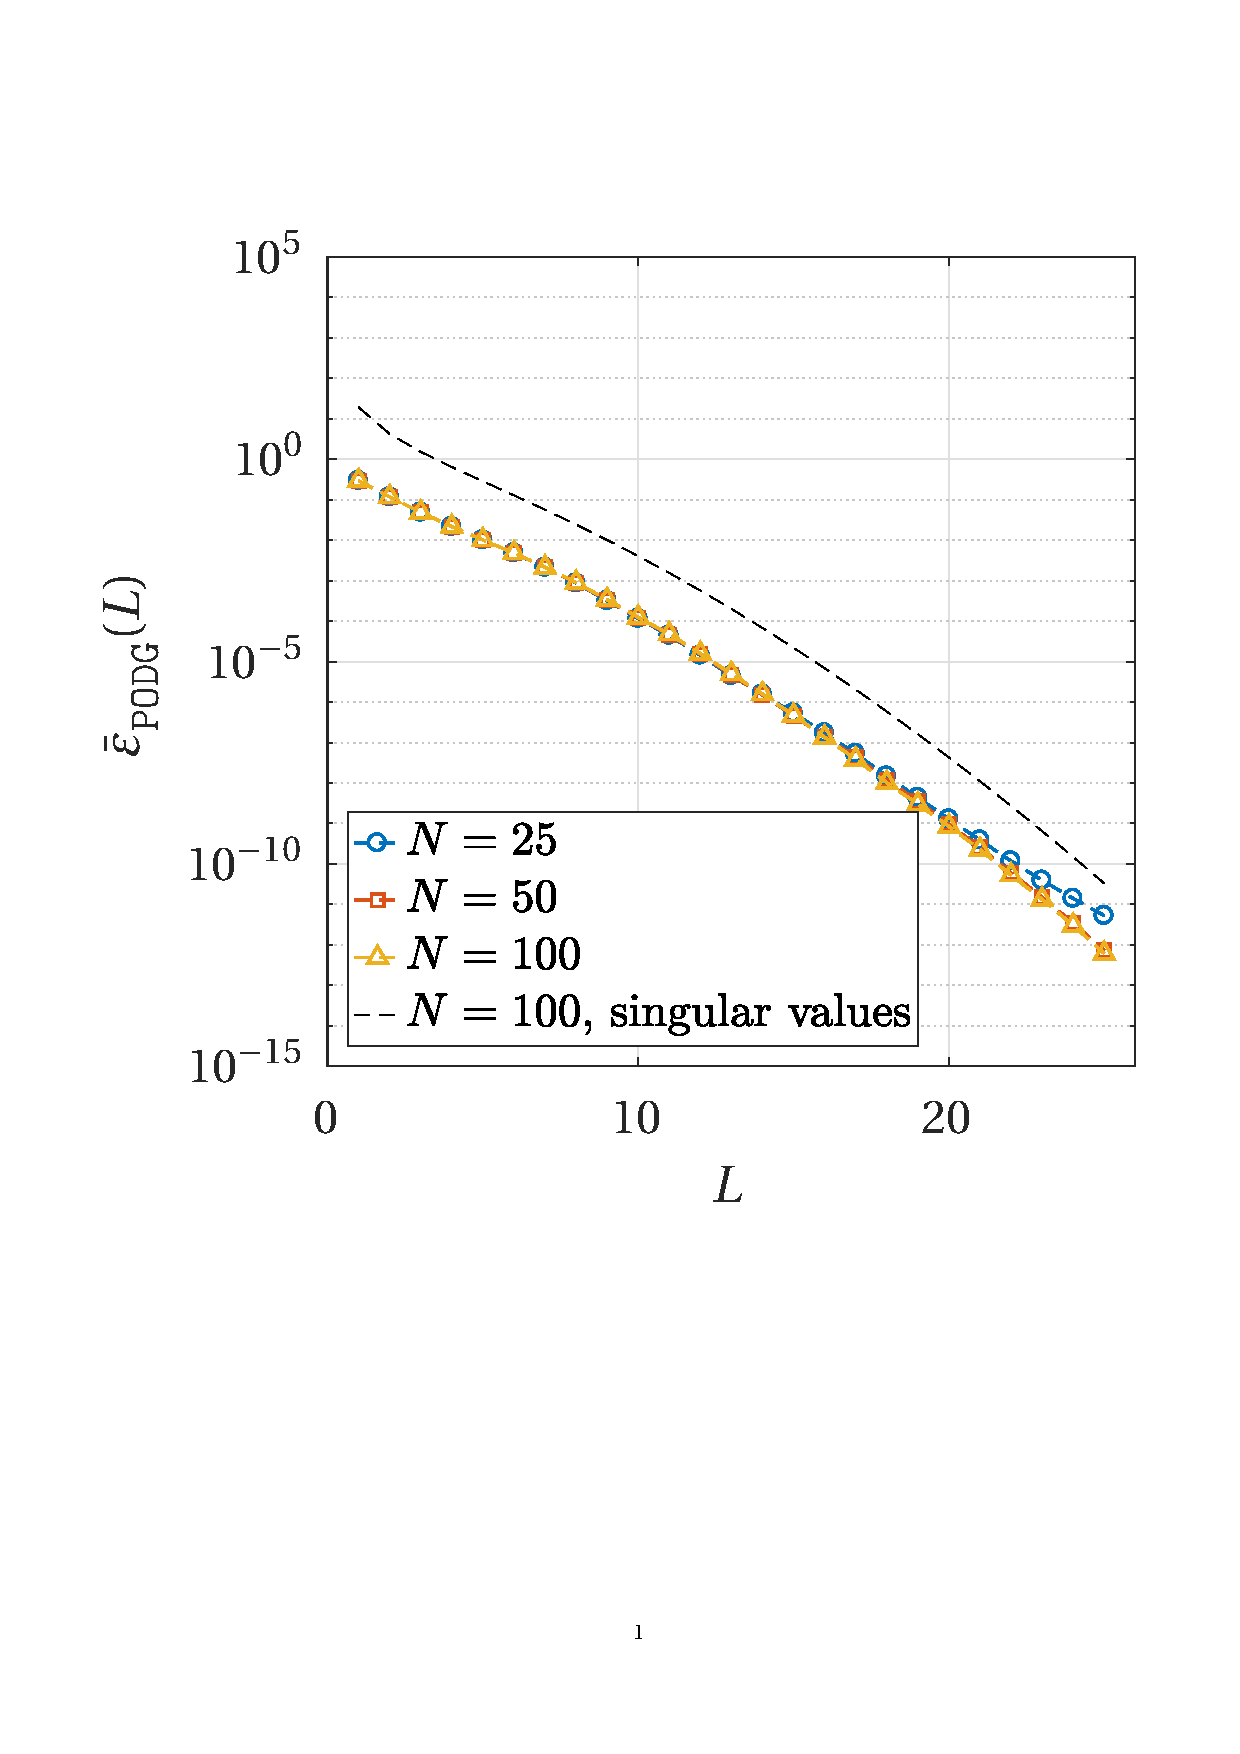
\includegraphics[scale = 0.41, trim = {1cm 9cm 1.5cm 3.5cm}, clip]{poisson1d_1_error_vs_rank}}
			\subfloat{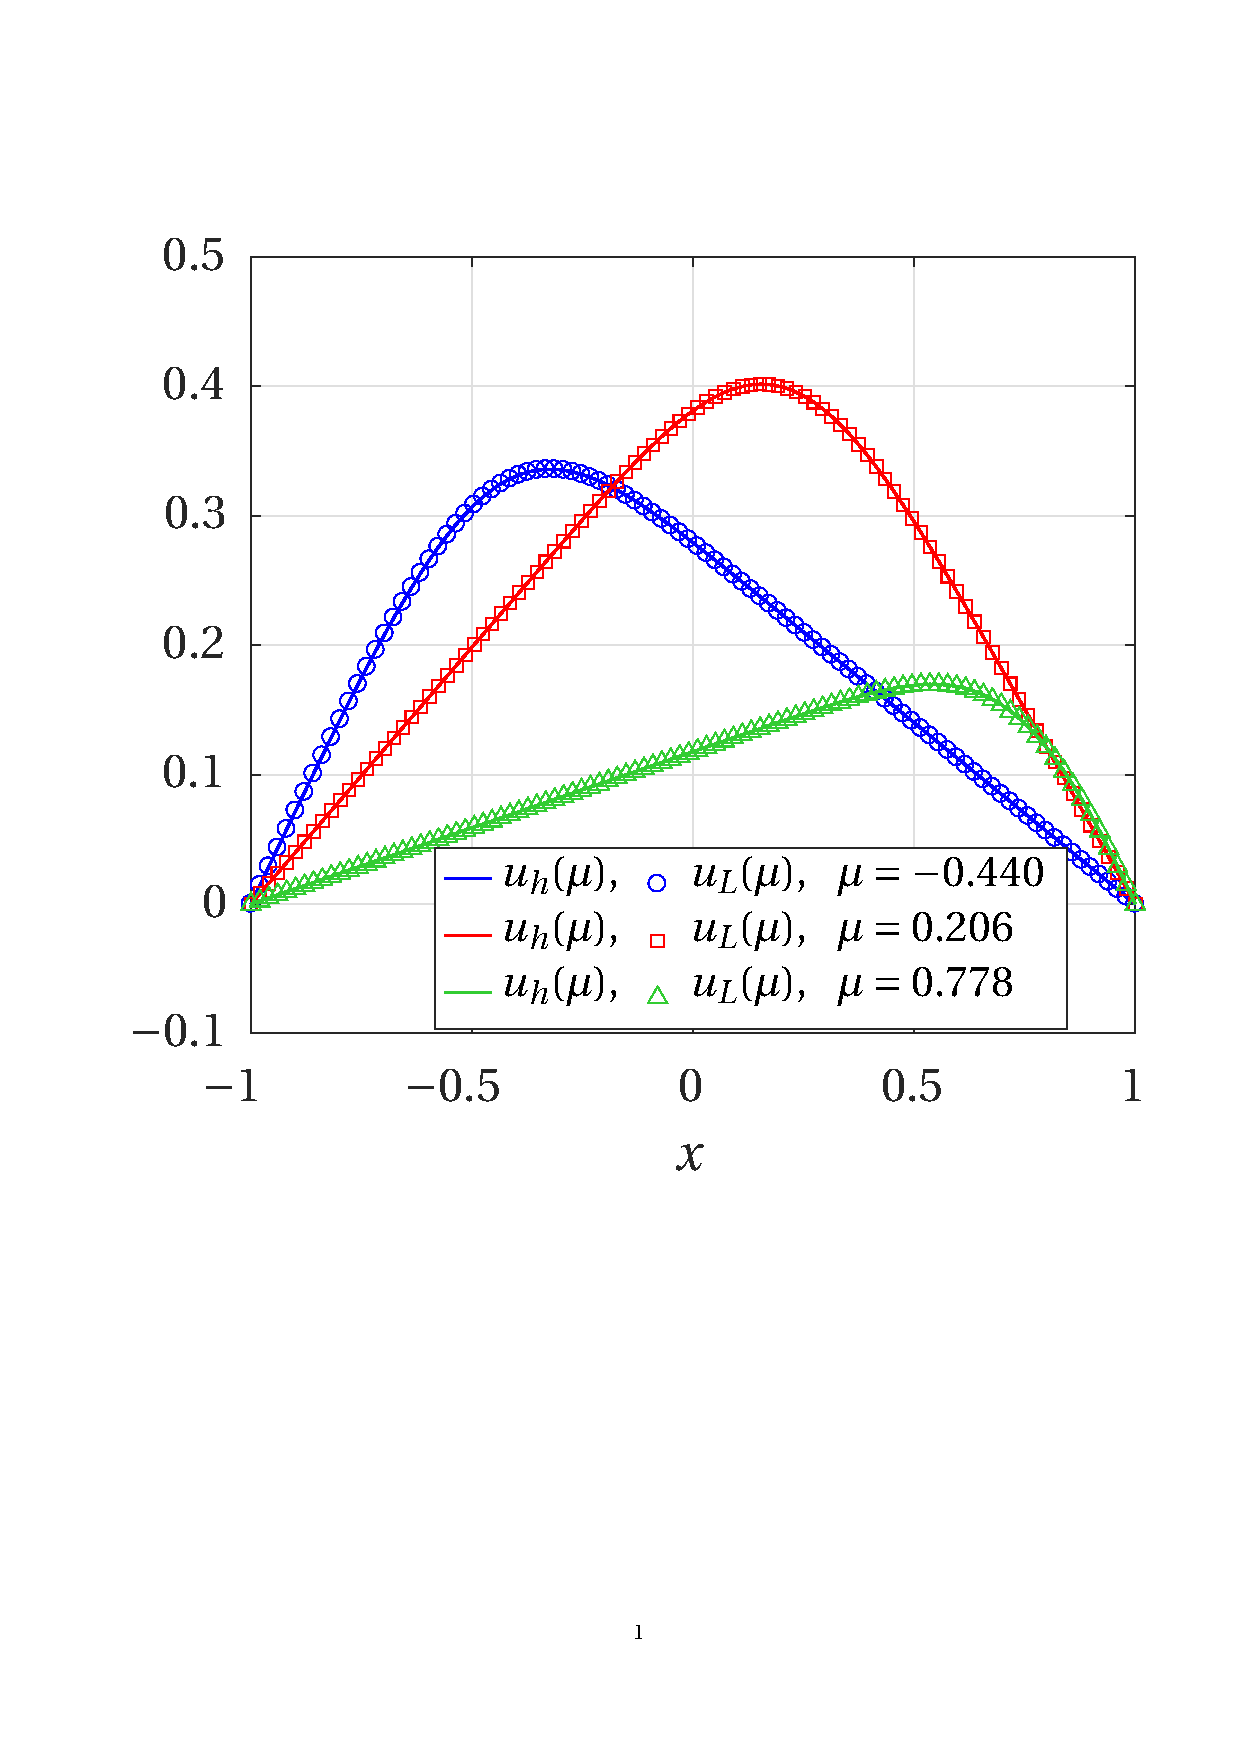
\includegraphics[scale = 0.41, trim = {1cm 9cm 1.5cm 3.5cm}, clip]{poisson1d_1_fe_vs_podg}}
			
			\caption{Left: error analysis for the POD-G RB method applied to \eqref{eq:poisson1d-1}; the results refer to a POD basis constructed based on $N = 25$, $50$, $100$ snapshots; for $N = 100$, the singular values of the corresponding snapshot matrix are shown as well. Right: FE and POD-G solutions for three parameter values.}
			\label{fig:poisson1d-1-fig1}
		\end{figure}
						
		\begin{figure}[t!]
			\center
			\subfloat{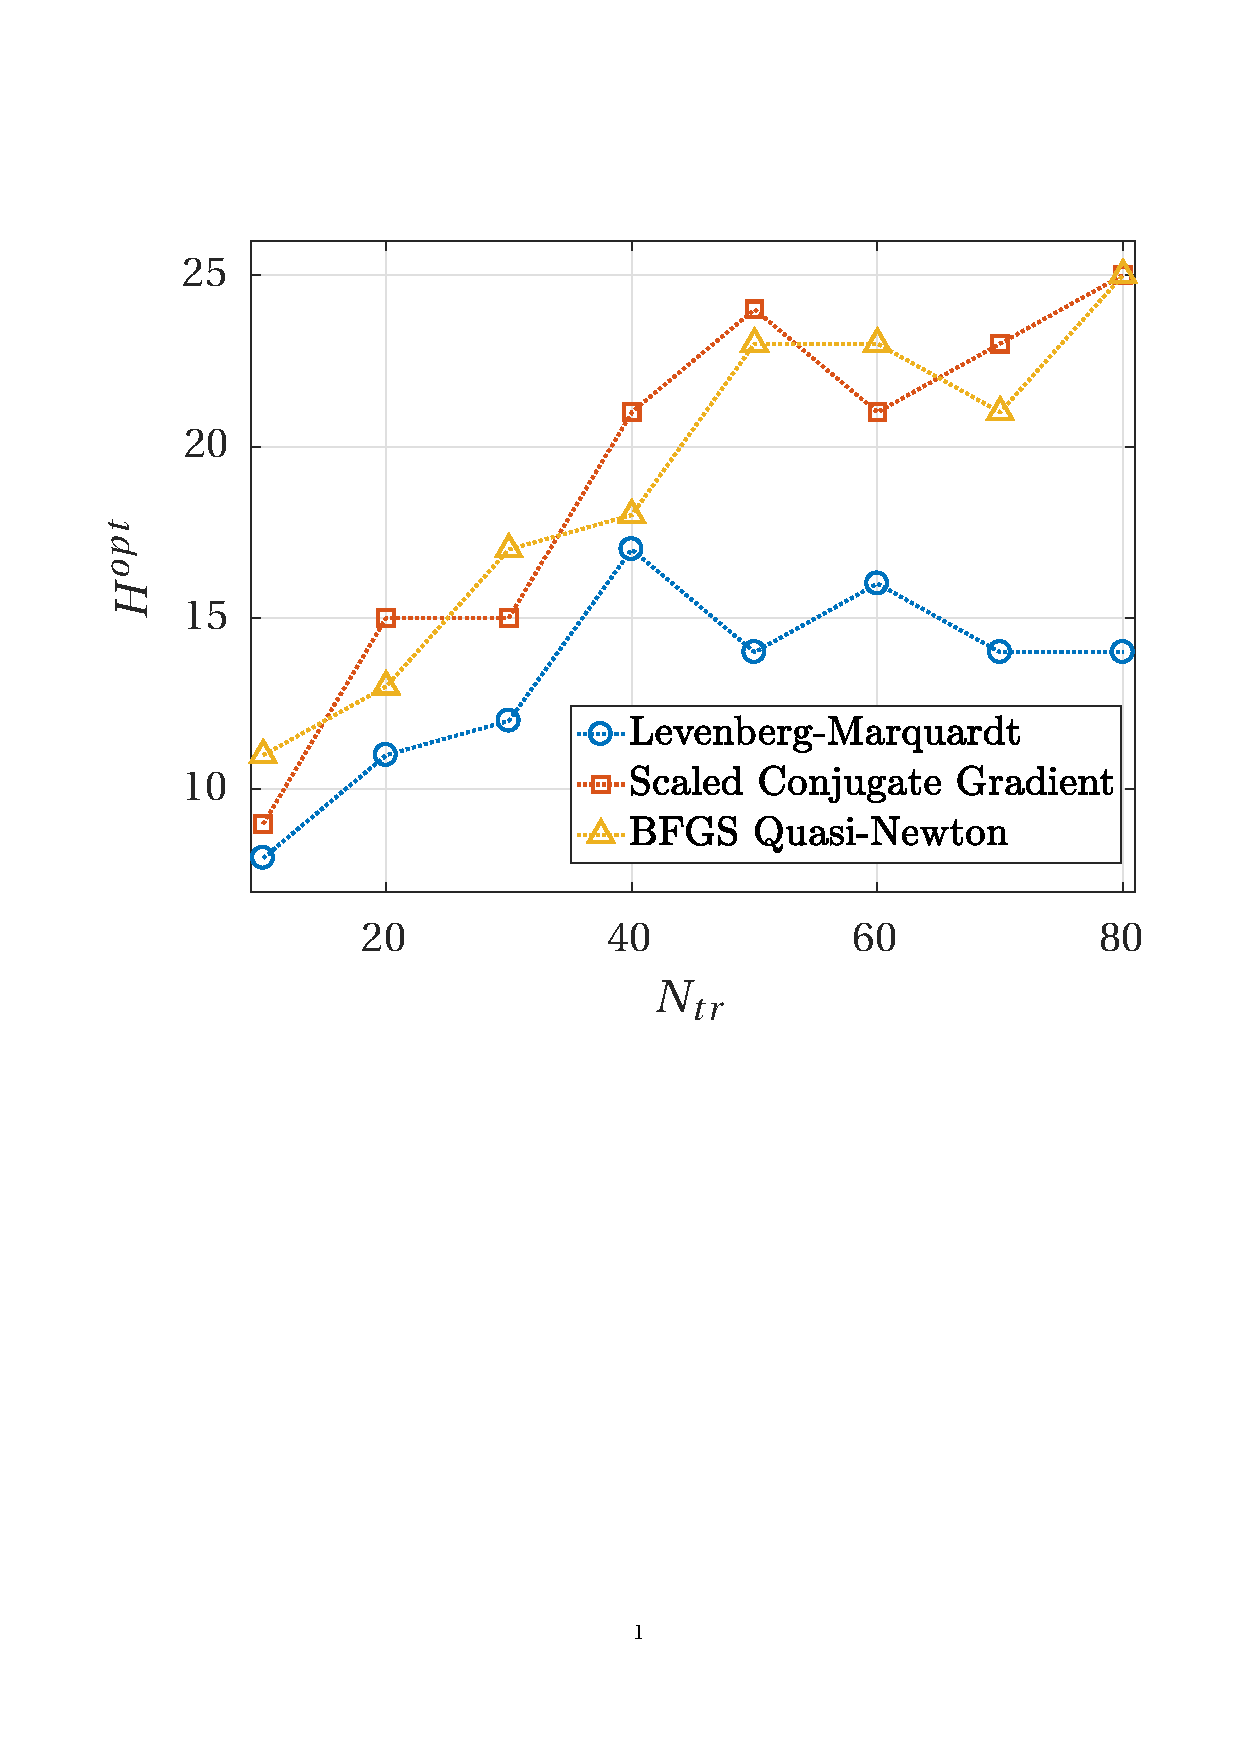
\includegraphics[scale = 0.42, trim = {1cm 12cm 1.5cm 3.5cm}, clip]{poisson1d_1_hopt}}
			\subfloat{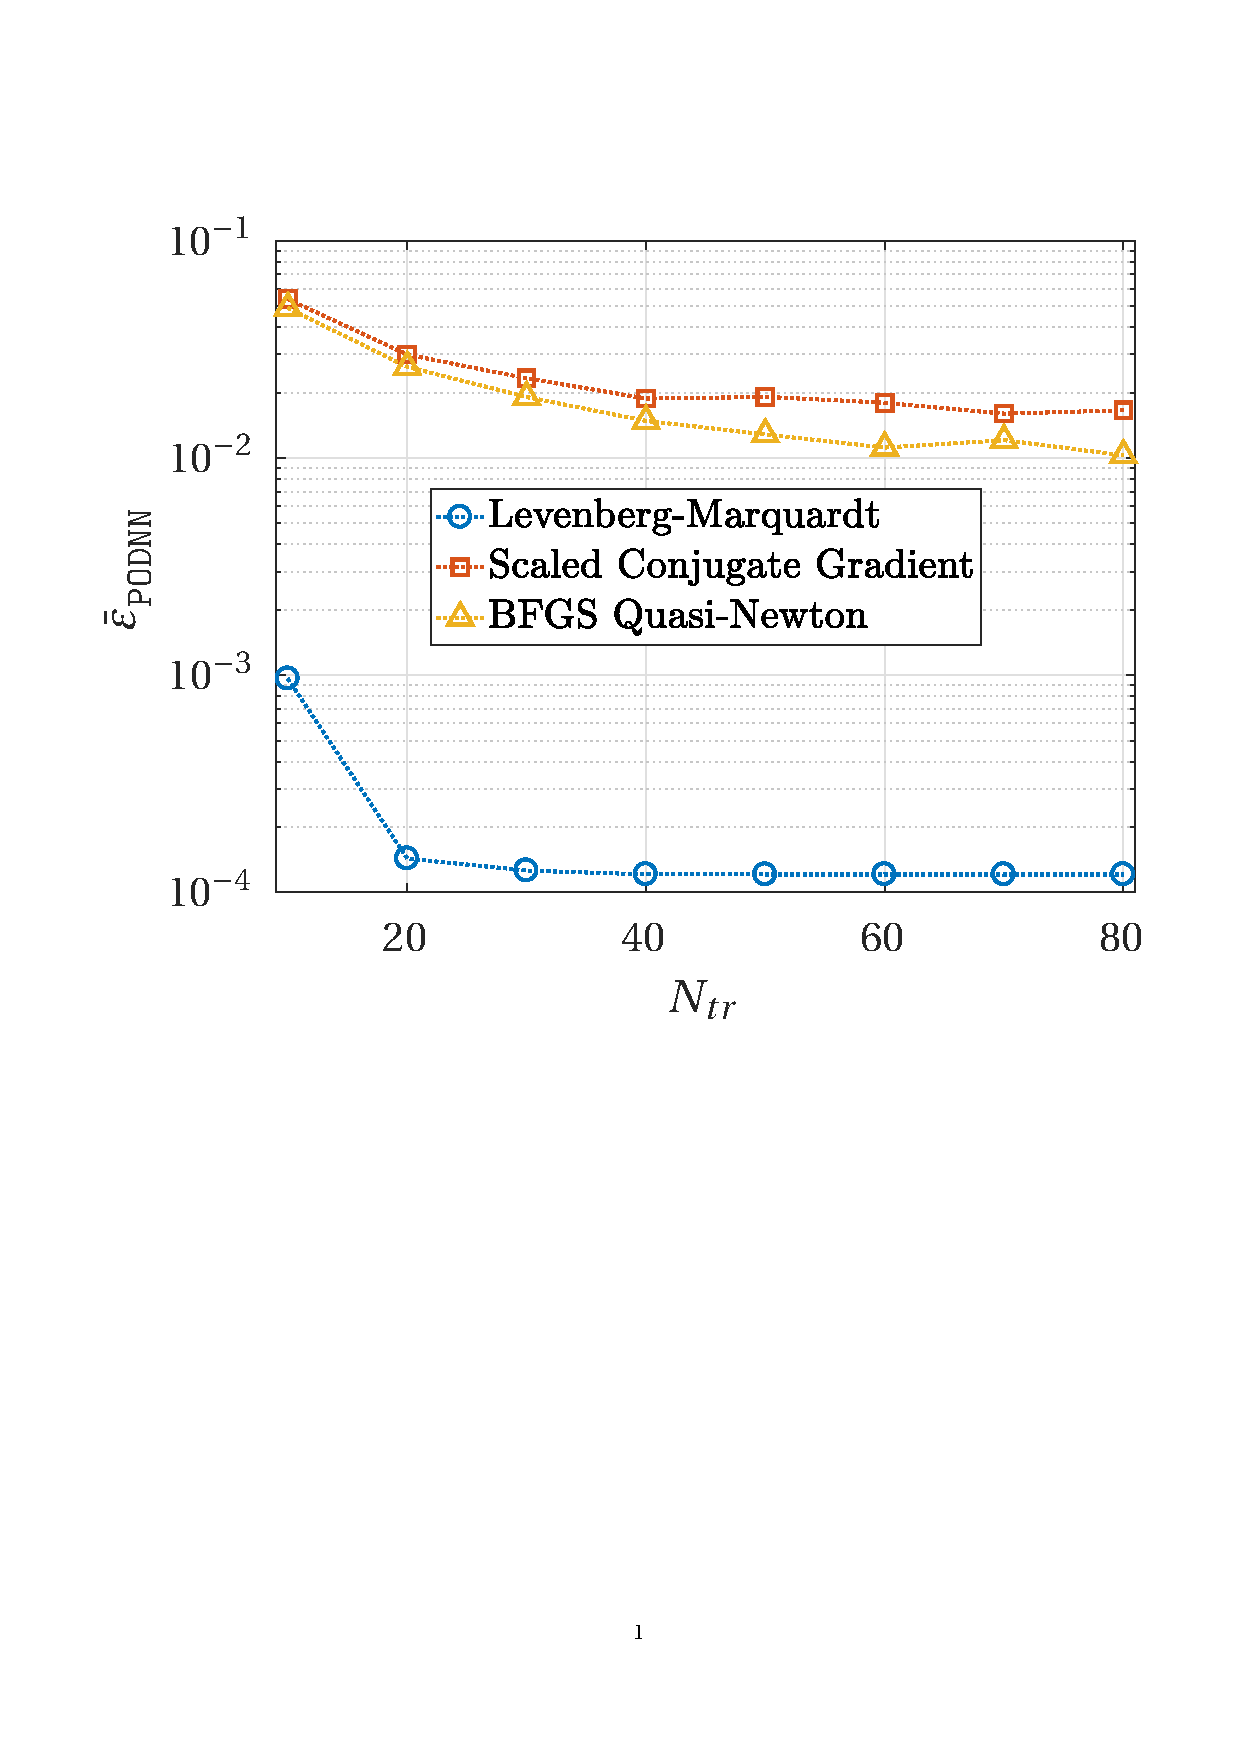
\includegraphics[scale = 0.42, trim = {1cm 12cm 1.5cm 3.5cm}, clip]{poisson1d_1_eopt}}
			
			\caption{In respect to the approximation of the map \eqref{eq:map-to-approximate} for the Poisson problem \eqref{eq:poisson1d-1} via neural networks, comparison between three supervised algorithms - Levenberg-Marquardt (blue circles), Scaled Conjugate Gradient (orange squares), BFGS Quasi-Newton (yellow traingles) - in terms of the optimal configuration detected (\emph{left}) and the associated (averaged) test error (\emph{right}) for different amounts of training samples.}
			\label{fig:poisson1d-1-fig2}
		
			\center
			\subfloat{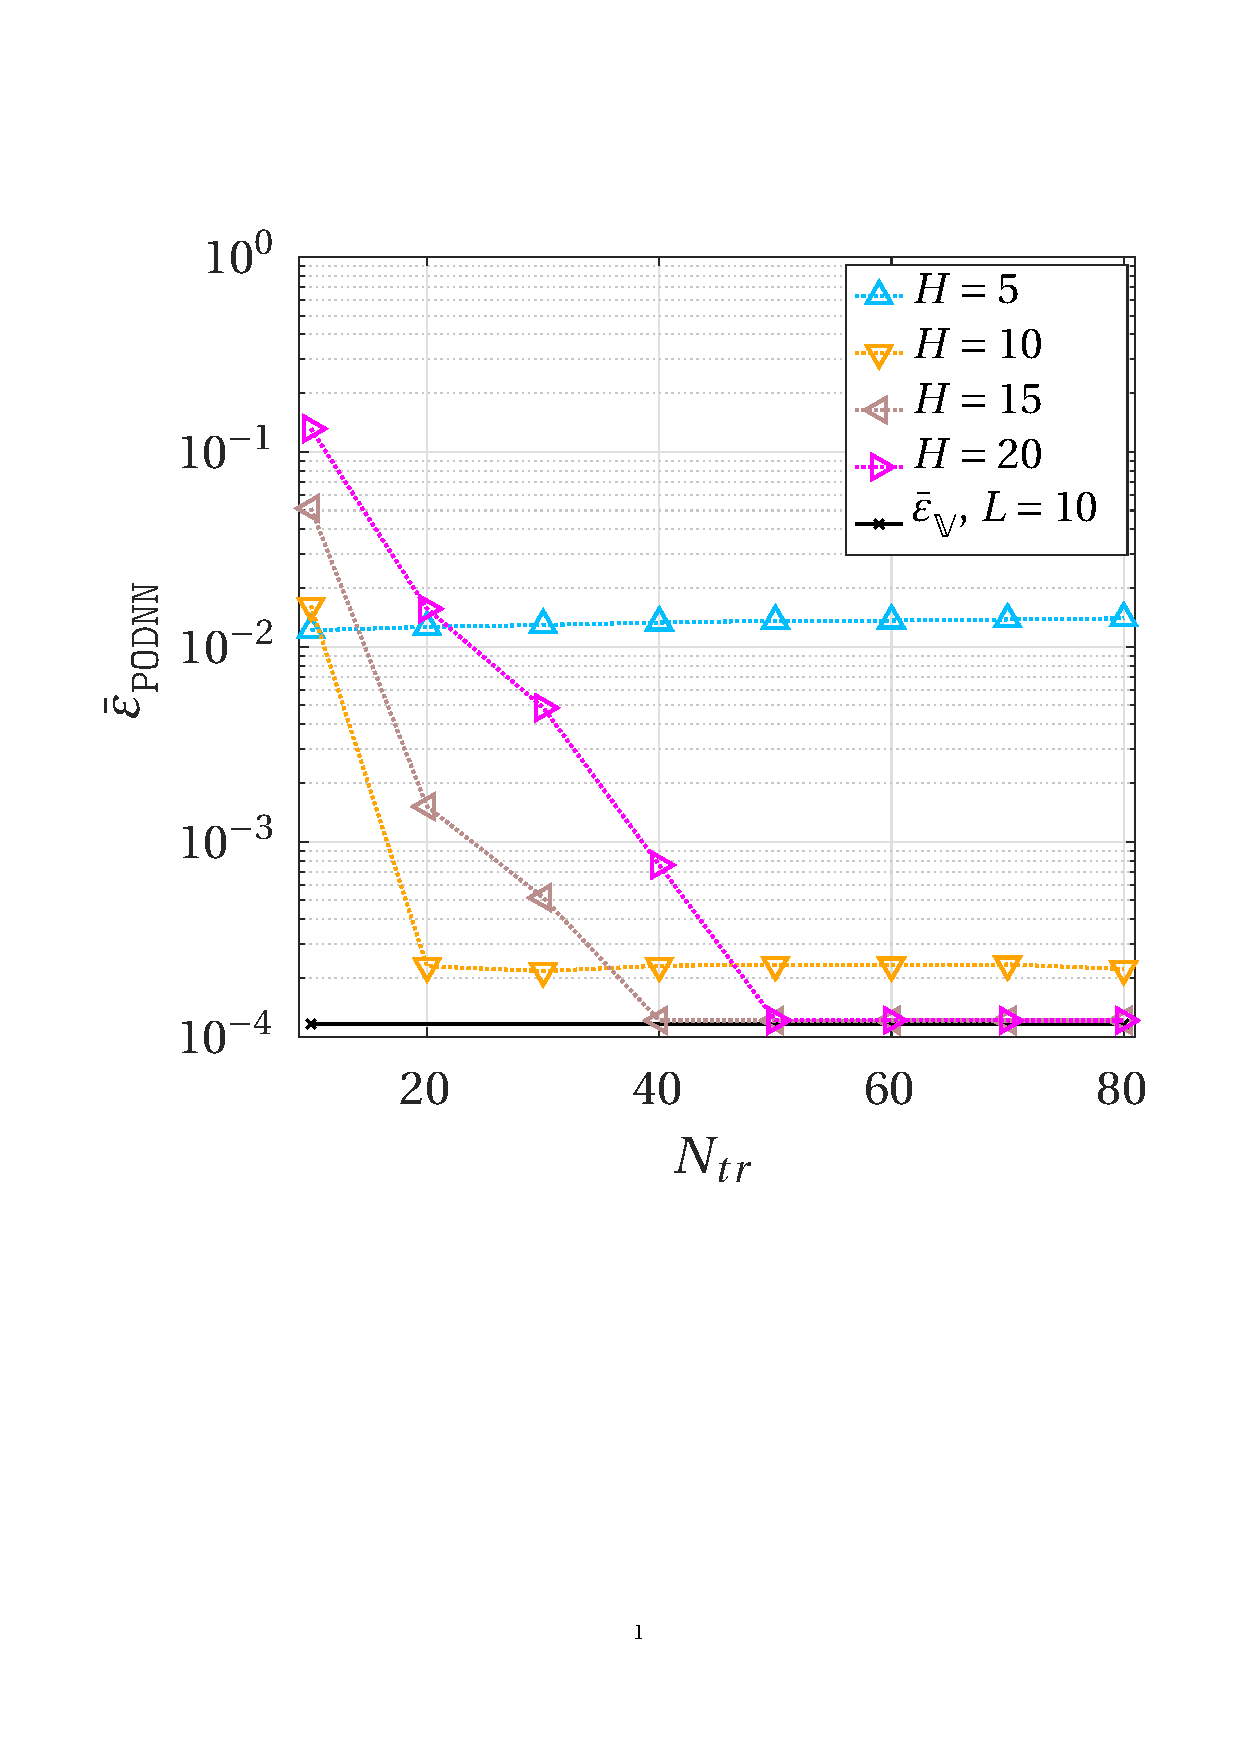
\includegraphics[scale = 0.42, trim = {1cm 9cm 1.5cm 3.5cm}, clip]{poisson1d_1_nn_convergence}}
			\subfloat{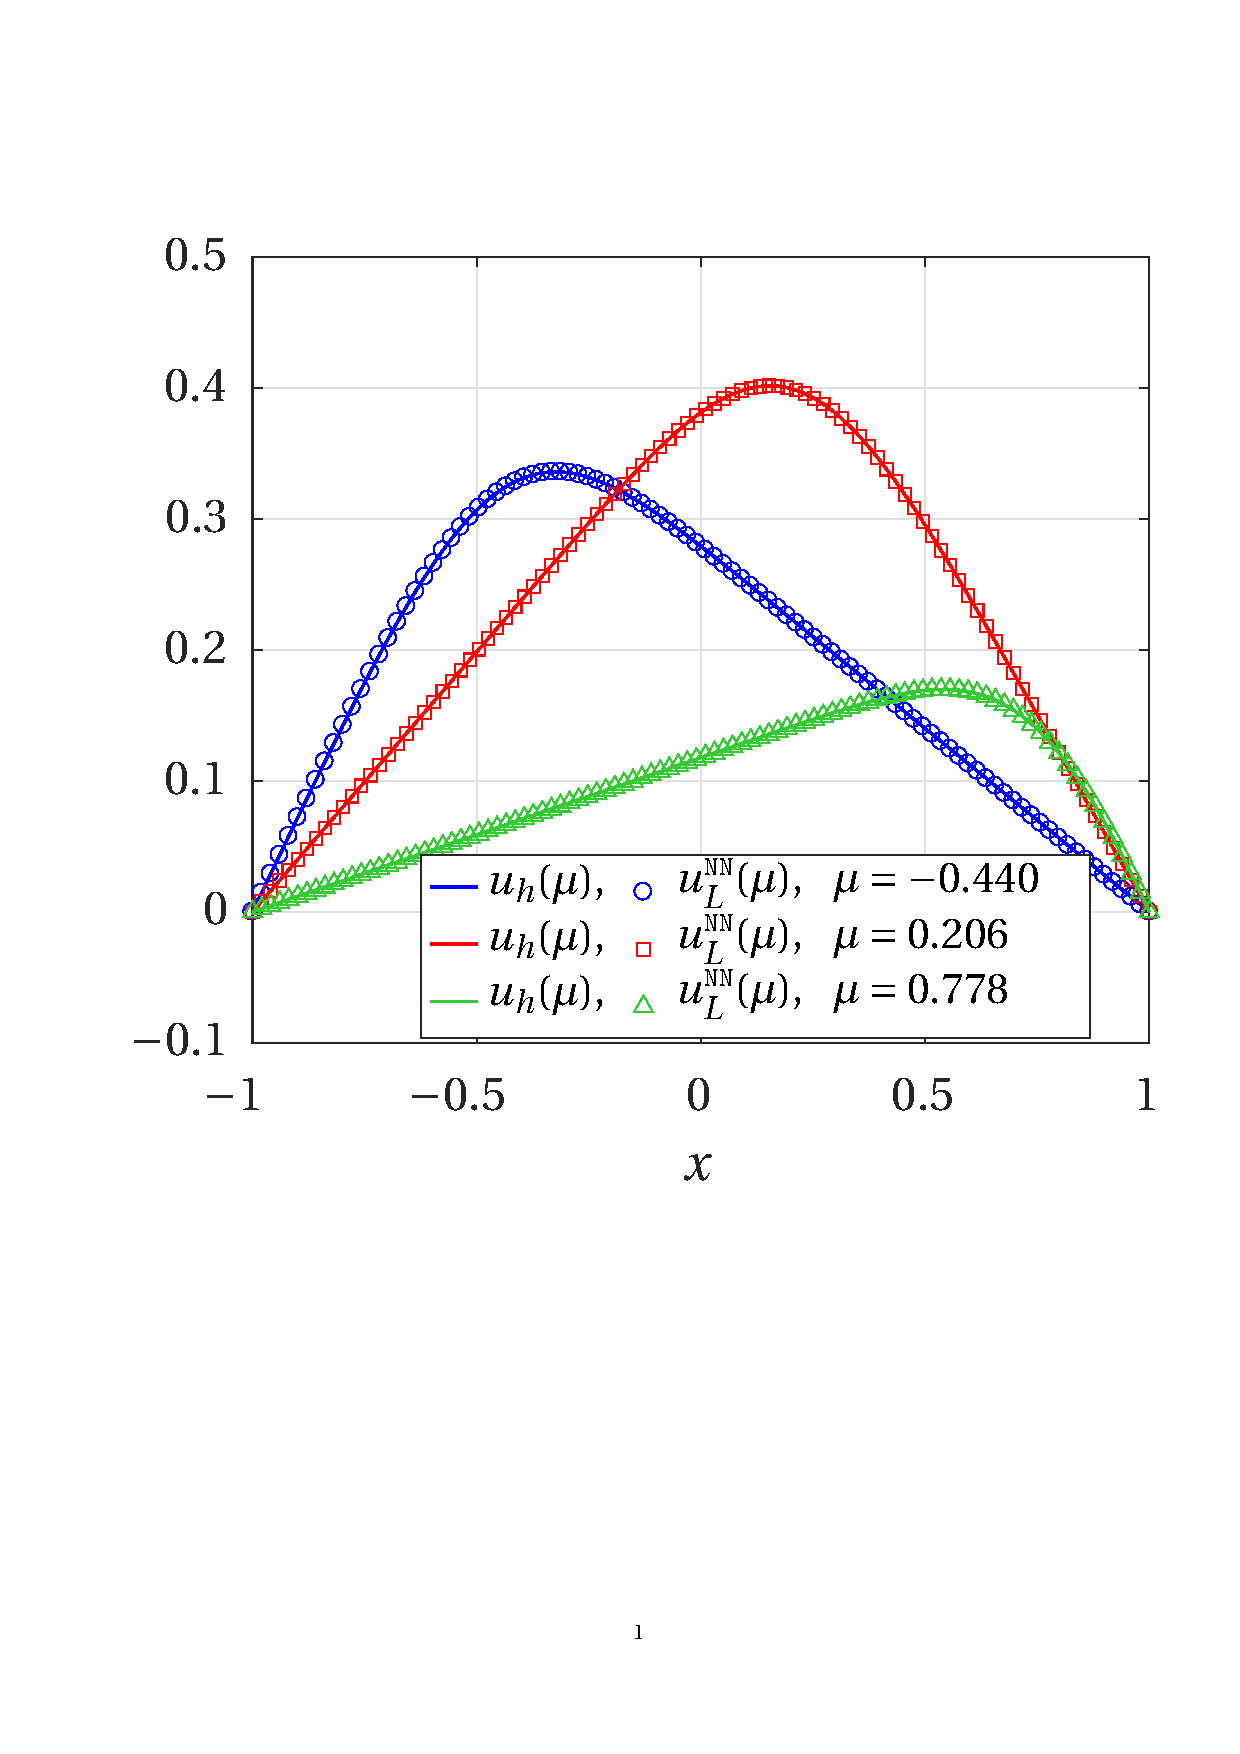
\includegraphics[scale = 0.42, trim = {1cm 9cm 1.5cm 3.5cm}, clip]{poisson1d_1_fe_vs_podnn}}
			
			\caption{Left: relative error yielded by the POD-NN RB method applied to \eqref{eq:poisson1d-1}; the convergence to the projection error for $L = 10$ (solid line) is analyzed in terms of both the number of neurons included in the neural network and the dimension of the training set. Right: FE and POD-NN solutions for three parameter values.}
			\label{fig:poisson1d-1-fig3}
		\end{figure}
		
		Moving to the analysis of the POD-NN method, we first seek to motivate the employment throughout this work of the Levenberg-Marquardt learning algorithm (see Section \ref{section:Levenberg-Marquardt algorithm}). To this end, we compare it against two other well-known and widely-used supervised training routines - the Scaled Conjugate Gradient \cite{Mol93} and the BFGS Quasi-Newton method \cite{GMW81} - on the regression of the map $\bg{\pi} = \bg{\pi}(\bg{\mu}) ~ : ~ \bg{\mu} \mapsto \mathbb{V}^T \mathbf{u}_h(\bg{\mu})$ (see also Eq. \eqref{eq:map-to-approximate}), with $L = 10$ POD modes, i.e., $\mathbb{V} \in \mathbb{R}^{M \times 10}$. In this simple linear case, we can limit ourselves to networks with a single hidden layer, embodying $H \in \big\lbrace 5, \, 10, \, 15, \, 20, \, 25 \big\rbrace$ inner neurons. Then, for a given number $N_{tr}$ of training samples, Fig. \ref{fig:poisson1d-1-fig2} tracks the number of hidden processing units required to yield the minimum error on $\Xi_{te}$ (\emph{left}) and the optimal error itself (\emph{right}) for each algorithm. We can observe that for any tested value of $N_{tr}$, the Levenberg-Marquardt algorithm (blue circles) leads to much more accurate approximations using fewer neurons. In other words, it turns out to be not only effective but even efficient. A confirmation of this is given by the plot on the left in Fig. \ref{fig:poisson1d-1-fig3}, showing the decay of the POD-NN error as the number of employed training patterns and neurons increases. Here, the lower-bound given by the projection error is actually attained via, e.g., a network with $H = 15$ hidden neurons, exposed to $N_{tr} = 40$ training samples. The solutions obtained by means of such network are provided in the right plot of Fig. \ref{fig:poisson1d-1-fig3}; note the substantial overlap with the corresponding FE solutions. 
				
	\subsection{Nonlinear test case, two parameters}
	\label{section:poisson1d-2}
	
		\begin{figure}[b!]
			\center
			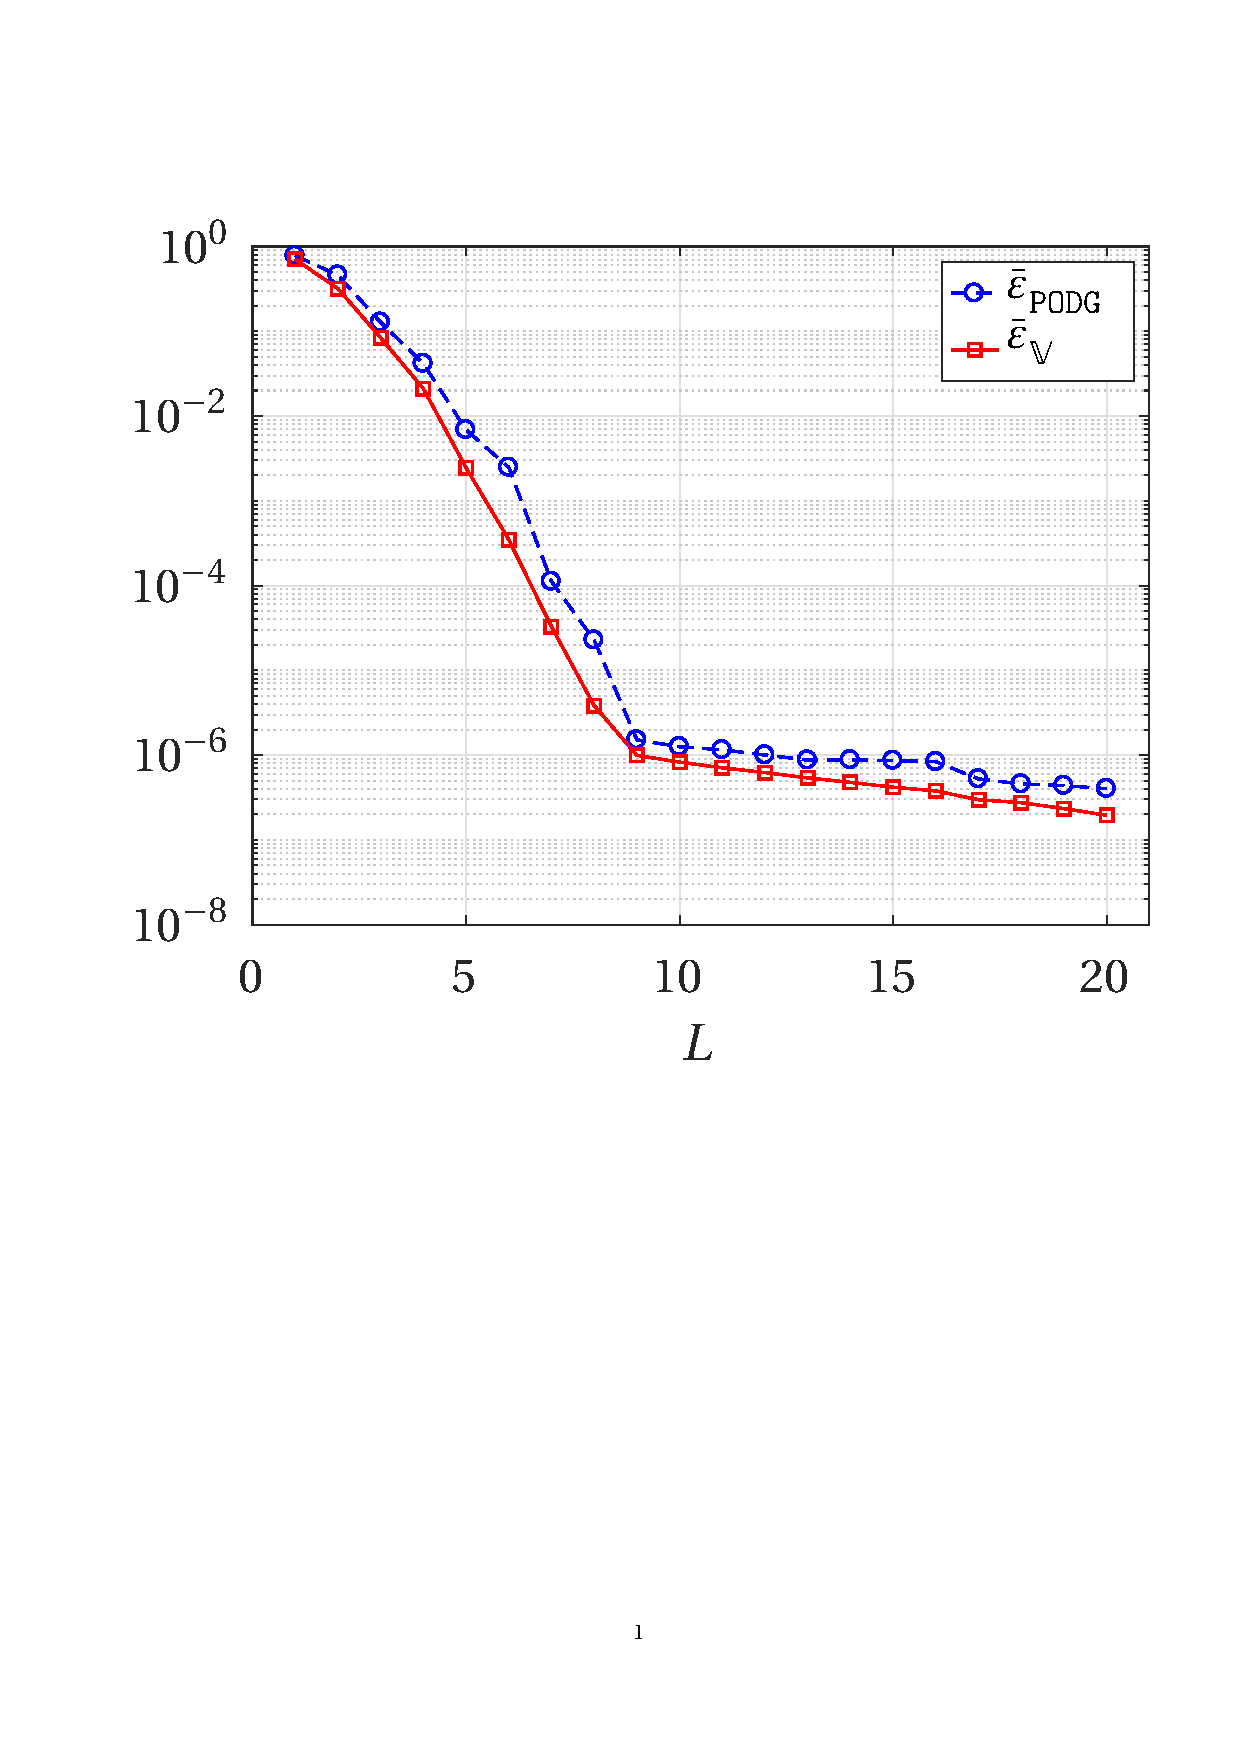
\includegraphics[scale = 0.43, trim = {1cm 10.5cm 1.5cm 3.5cm}, clip]{poisson1d_2_error_vs_rank}
			
			\caption{Error analysis for the POD-Galerkin RB method applied to the problem \eqref{eq:poisson1d-2}. The lower-bound provided by the projection error \eqref{eq:projection-error} is reported as reference.}
			\label{fig:poisson1d-2-fig1}
		\end{figure}
	
		The first nonlinear problem we consider reads:
		\begin{equation}
			\label{eq:poisson1d-2}
			\begin{cases}
				& - \left( \big( 1 + u(\bg{\mu})^2 \big) ~ u(\bg{\mu})' \right)' = s(x; \, \bg{\mu}) \hspace*{0.3cm} \text{in $\Omega = [-\pi, \, \pi]$} \, , \\
				& u(\bg{\mu}) \big|_{x = -\pi} = \mu_2 \sin(2 - \mu_1 \, \pi) \, , \hspace*{0.3cm} u(\bg{\mu}) \big|_{x = \pi} = \mu_2 \sin(2 + \mu_1 \, \pi)  \, ,
			\end{cases}
		\end{equation}
		where $\bg{\mu} = \big( \mu_1, \, \mu_2 \big) \in \mathcal{P} = [1, \, 3] \times [1, \, 3]$ and the source term $s(x; \, \bg{\mu})$ is chosen so that $u_{ex}(x; \, \bg{\mu}) = \mu_2 \sin(2 + \mu_1 \, x)$ represents the exact solution to the problem for any $\bg{\mu} \in \mathcal{P}$. Here, a POD-Galerkin RB model built upon $N = 50$ samples (randomly picked via LHS) turns out to be highly effective. Indeed, as reported by Fig. \ref{fig:poisson1d-2-fig1}, the yielded relative error, averaged over $N_{te} = 100$ samples, rapidly decades as the amount $L$ of retained POD basis functions increases, attaining a value of $10^{-7}$ already for $L = 15$. Hence, the design of an effective neural network, which can at least approach the accuracy provided by the algebraic ROM, is really challenging. The results concerning the search for an optimal three-layers network configuration via the methodology described in Algorithm \ref{alg:podnn-training} are provided on the left in Fig. \ref{fig:poisson1d-2-fig2}. The steps pursued by the routine are represented through solid tracts. However, for the sake of completeness, we also report the test error (understood as the minimum over multiple restarts) for any considered value for both the number of hidden neurons per layer ($H_1$ and $H_2$) and the dimension of the training set ($N_{tr}$). 
		
		\begin{figure}[t!]
			\center
			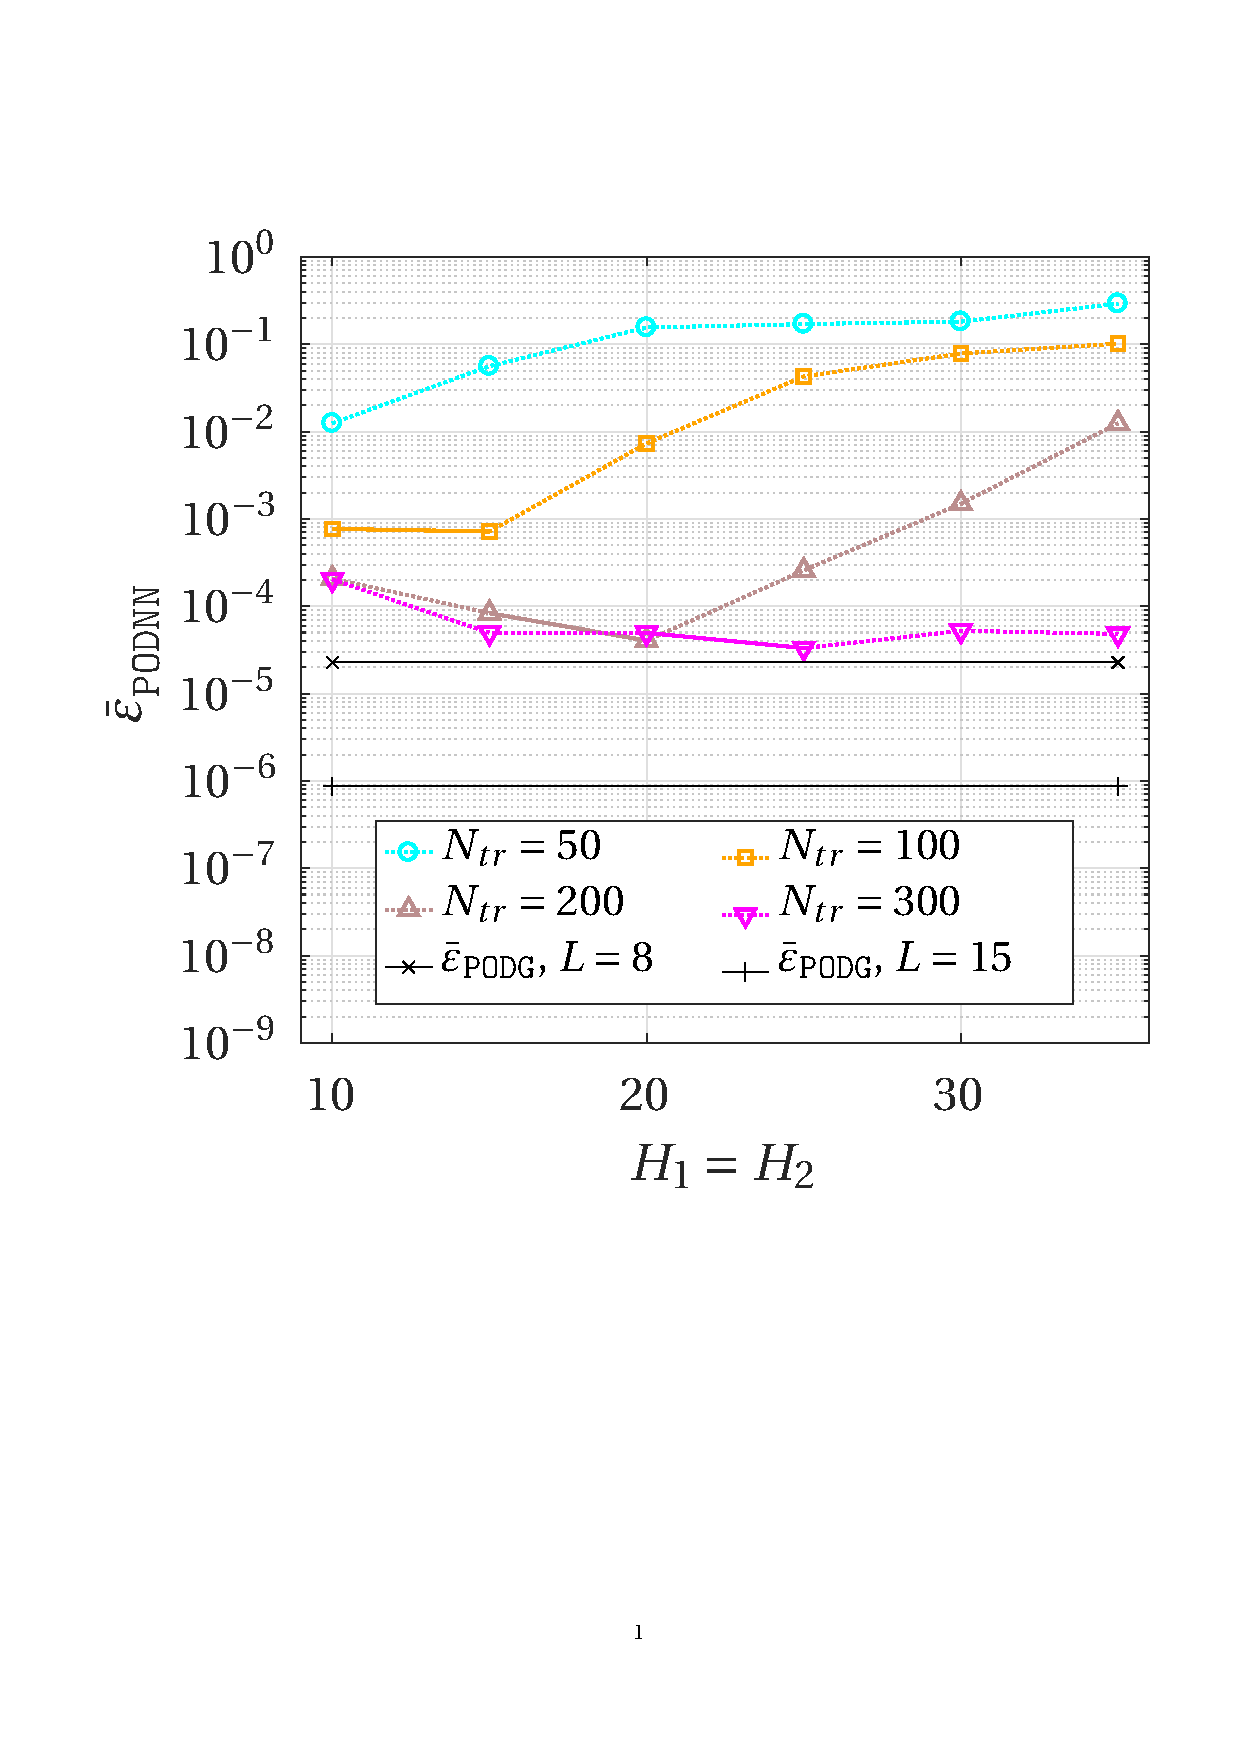
\includegraphics[scale = 0.42, trim = {1cm 9cm 1.5cm 3.5cm}, clip]{poisson1d_2_nn_convergence}
			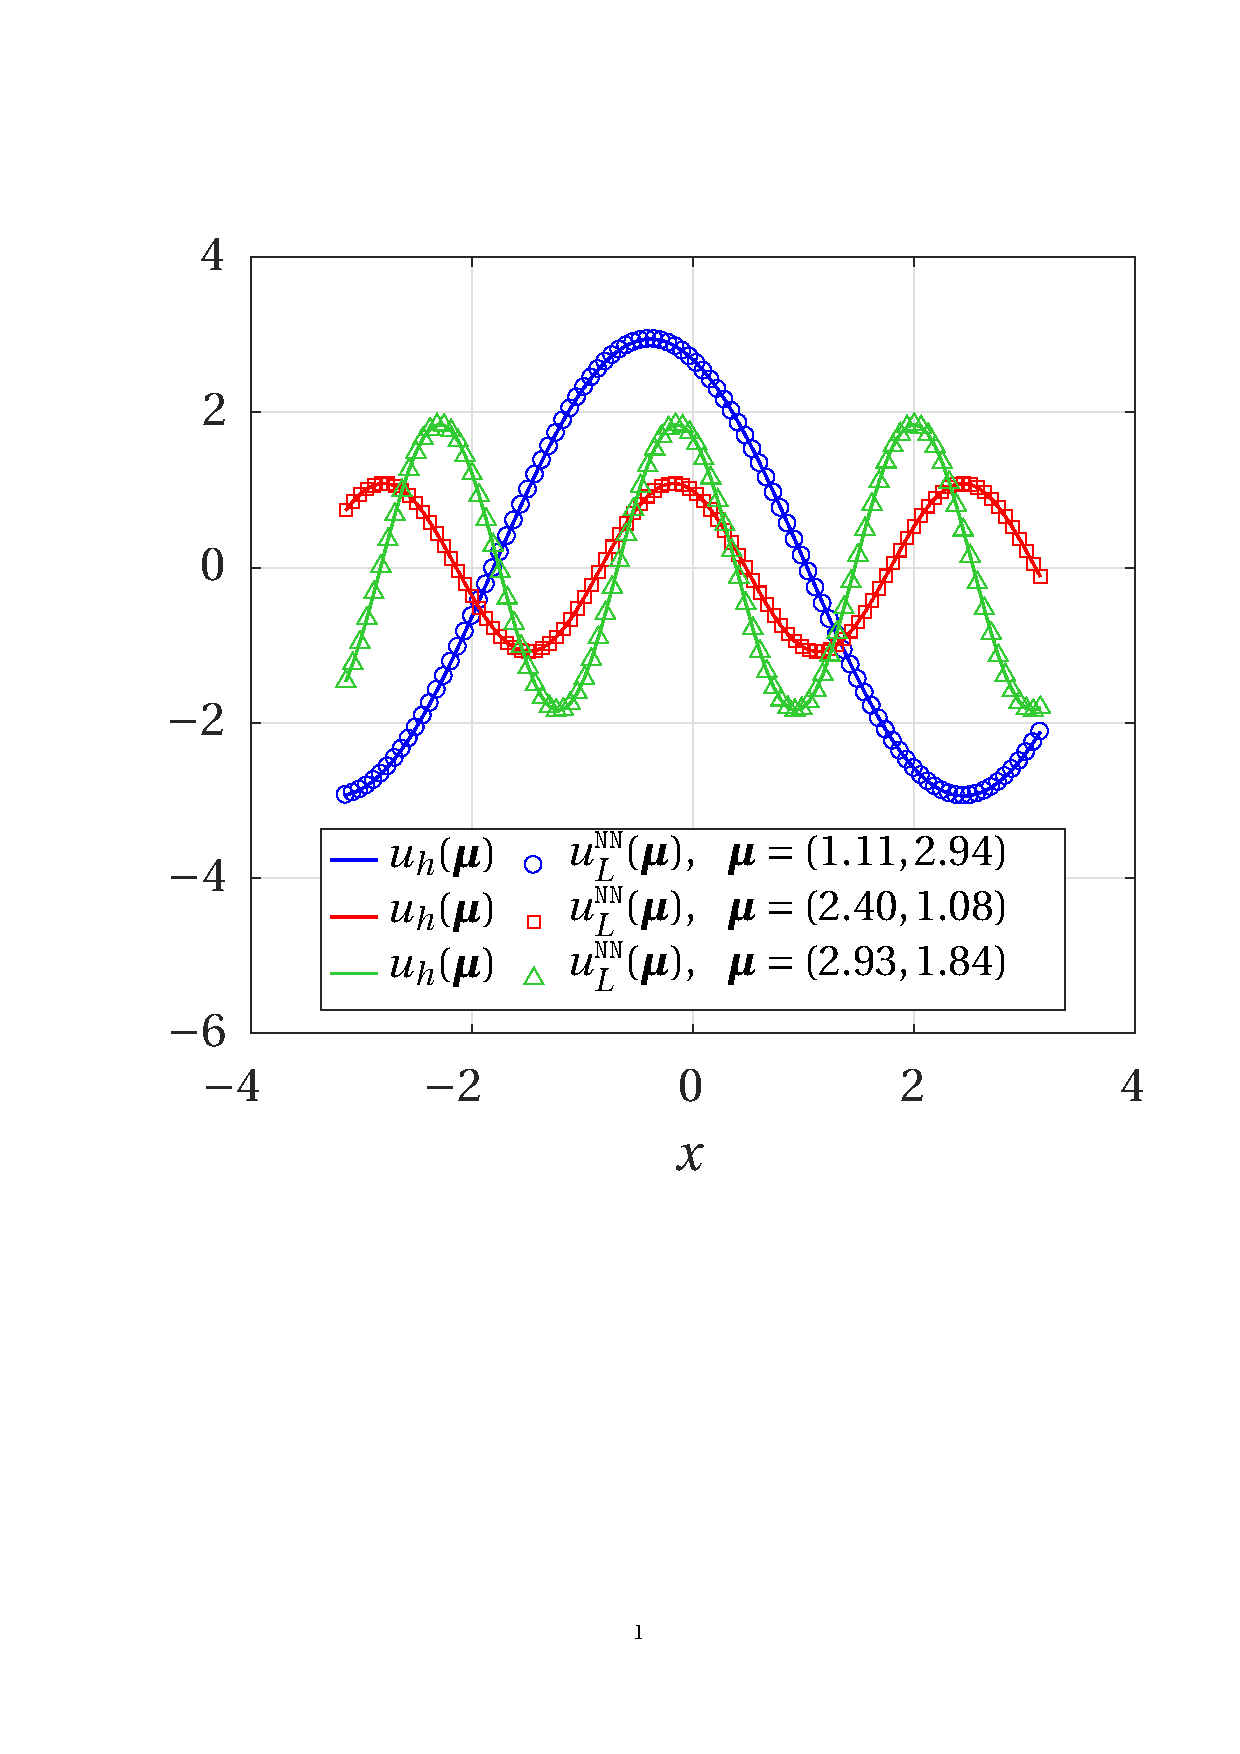
\includegraphics[scale = 0.42, trim = {1cm 9cm 1.5cm 3.5cm}, clip]{poisson1d_2_fe_vs_podnn}
			
			\caption{Left: error analysis for the POD-NN RB method (dotted lines) applied to problem \eqref{eq:poisson1d-2}. The solid solid sections refer to the steps carried out by the routine \ref{alg:podnn-training}; the error yielded by the POD-G method using $L = 8$ or $L = 15$ basis functions are reported as reference. Right: comparison between FE and POD-NN solutions for three input vectors.}
			\label{fig:poisson1d-2-fig2}
		\end{figure}
		
		Let us first point out that the basic assumption which Algorithm \ref{alg:podnn-training} relies on is fulfilled: as the number of available samples increases, the amount of neurons which allows to attain the minimum of the error increases as well, while the minimum itself decreases. However, although the networks have been trained to approximate $L = 15$ projection coefficients, we can not guarantee the same precision provided by the POD-G method retaining the same quantity of basis functions. Instead, we get the same level of accuracy offered by POD-G employing only $L = 8$ basis vectors. To get some insights on this, consider the regression plots in Fig. \ref{fig:poisson1d-2-fig3}, comparing, for an MLP with $H_1 + H_2 = 50$ hidden neurons and for each test sample in $\Xi_{te}$, some of the components of the network output with the corresponding target expansion coefficients. While the first and seventh coefficients (\emph{top}) are interpolated almost exactly, problems start arising for the eighth (\emph{bottom left}) and mainly for the nineth (\emph{bottom right}) ones. This suggests that the Levenberg-Marquardt algorithm is sufficiently \emph{smart} to detect that the average magnitude of a projection coefficient decreases with the ordinality of the coefficient itself \footnote{This observation follows from the fact that the energy retained by each POD mode $\bg{\psi}_i$ is monotonically decreasing in $i$.}, and so that particular effort should be put in a proper regression of the first generalized coordinates. Indeed, although the prediction for the nineth entry of the vector $\mathbb{V}^T \mathbf{u}_h(\bg{\mu})$ is completely off in most of the cases, the average value of this component is around $10^{-4}$. As a result, the global solution provided by the network turns out to be really close to the corresponding FE discretization, as shown in Fig. \ref{fig:poisson1d-2-fig2} (\emph{right}).
		
		\clearpage
				
		\begin{figure}[t!]
			\center
			\subfloat{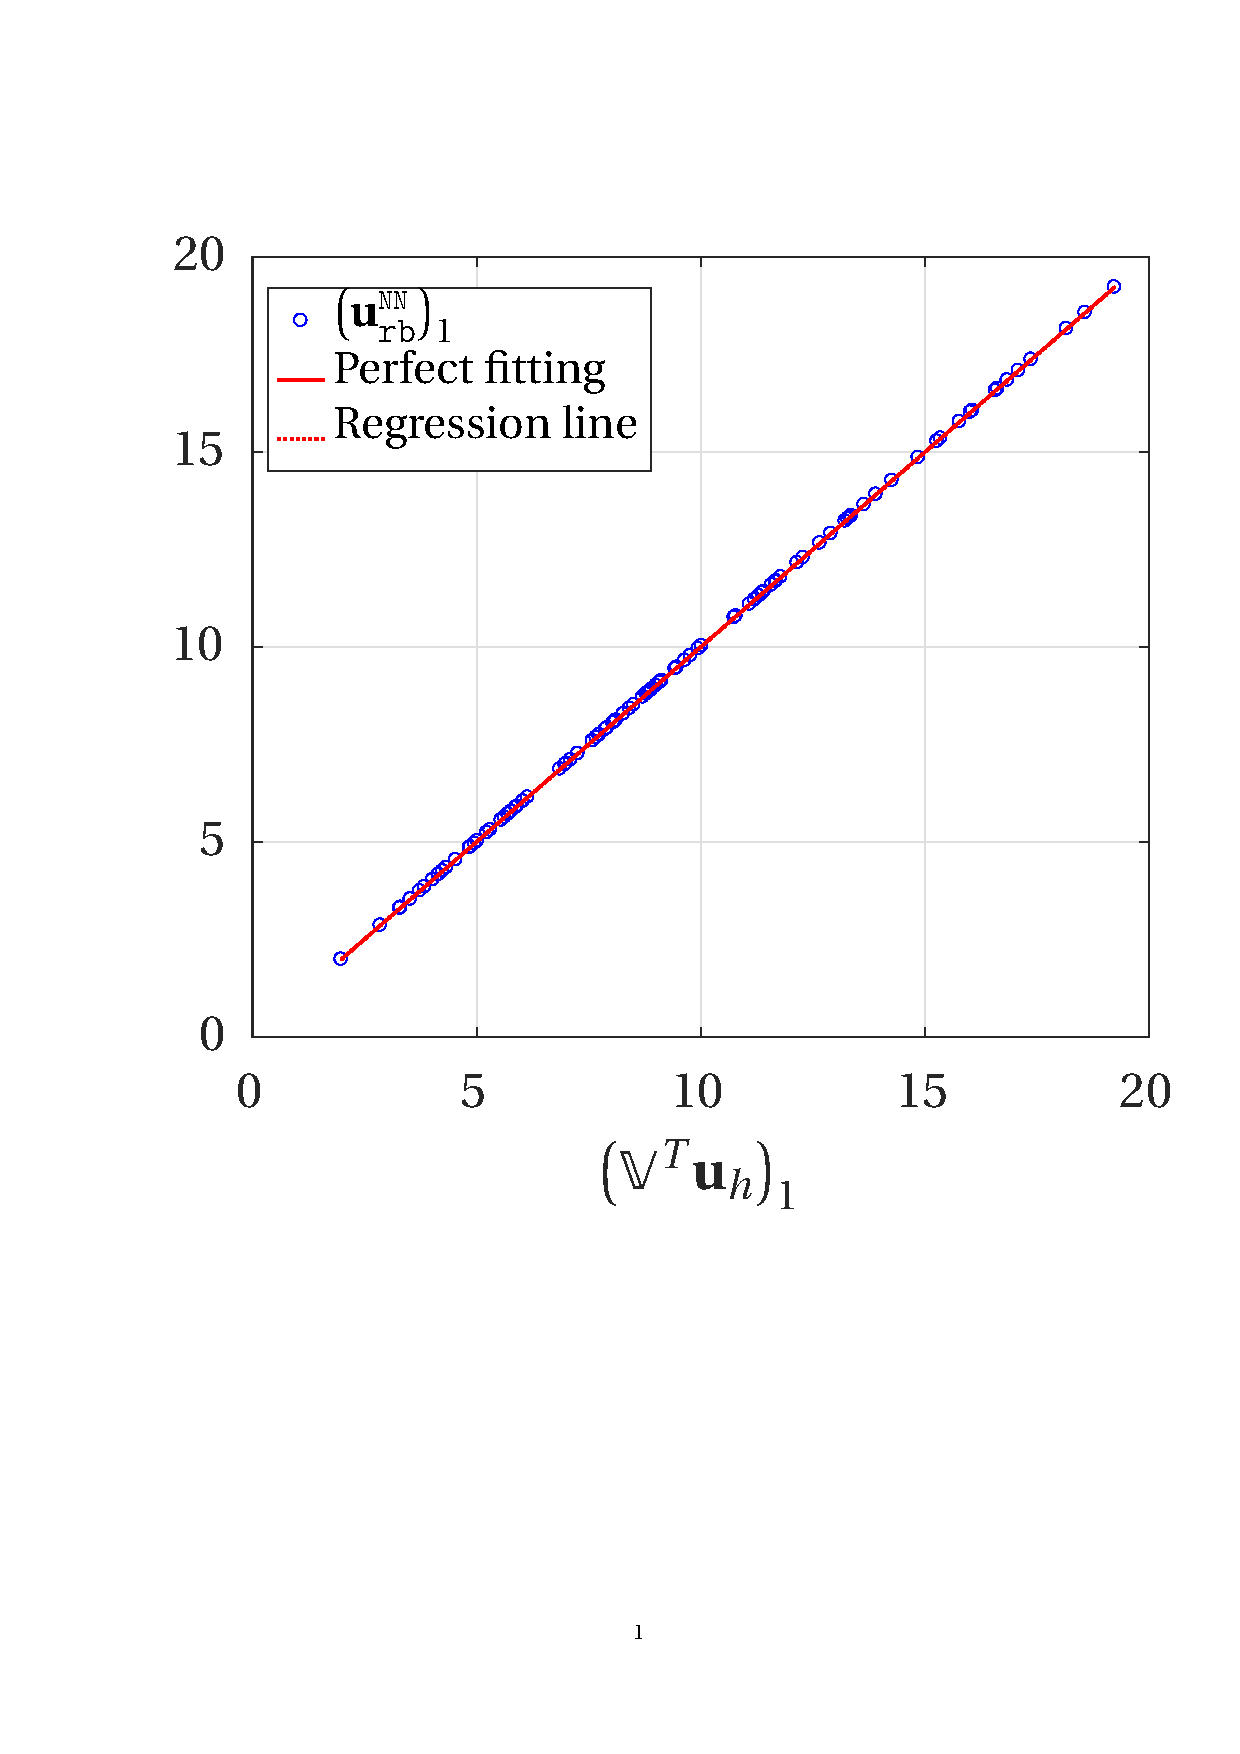
\includegraphics[scale = 0.4, trim = {1cm 9cm 1cm 3.5cm}, clip]{poisson1d_2_regression_1}}
			\subfloat{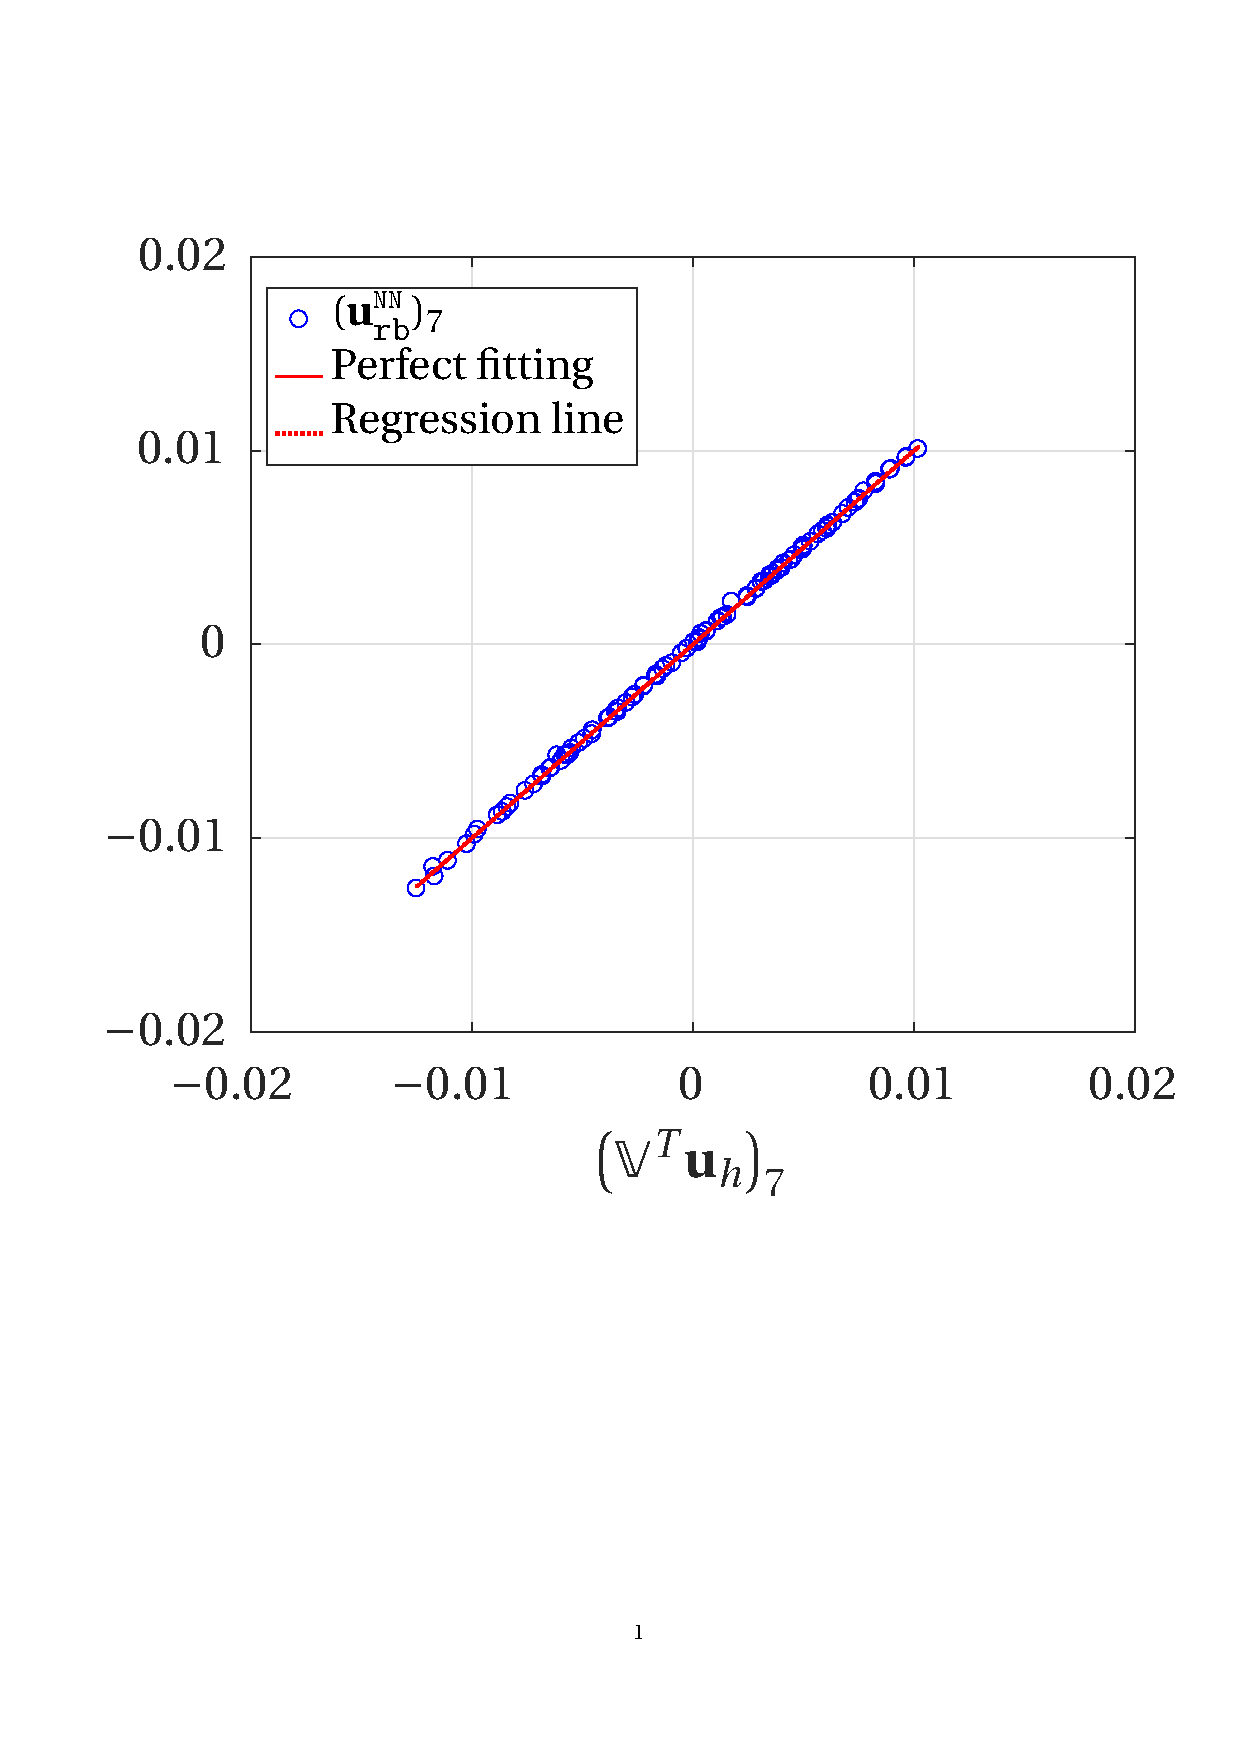
\includegraphics[scale = 0.4, trim = {1cm 9cm 1cm 3.5cm}, clip]{poisson1d_2_regression_7}} \\
			\vspace*{-1cm}
			\hspace*{0.1cm}
			\subfloat{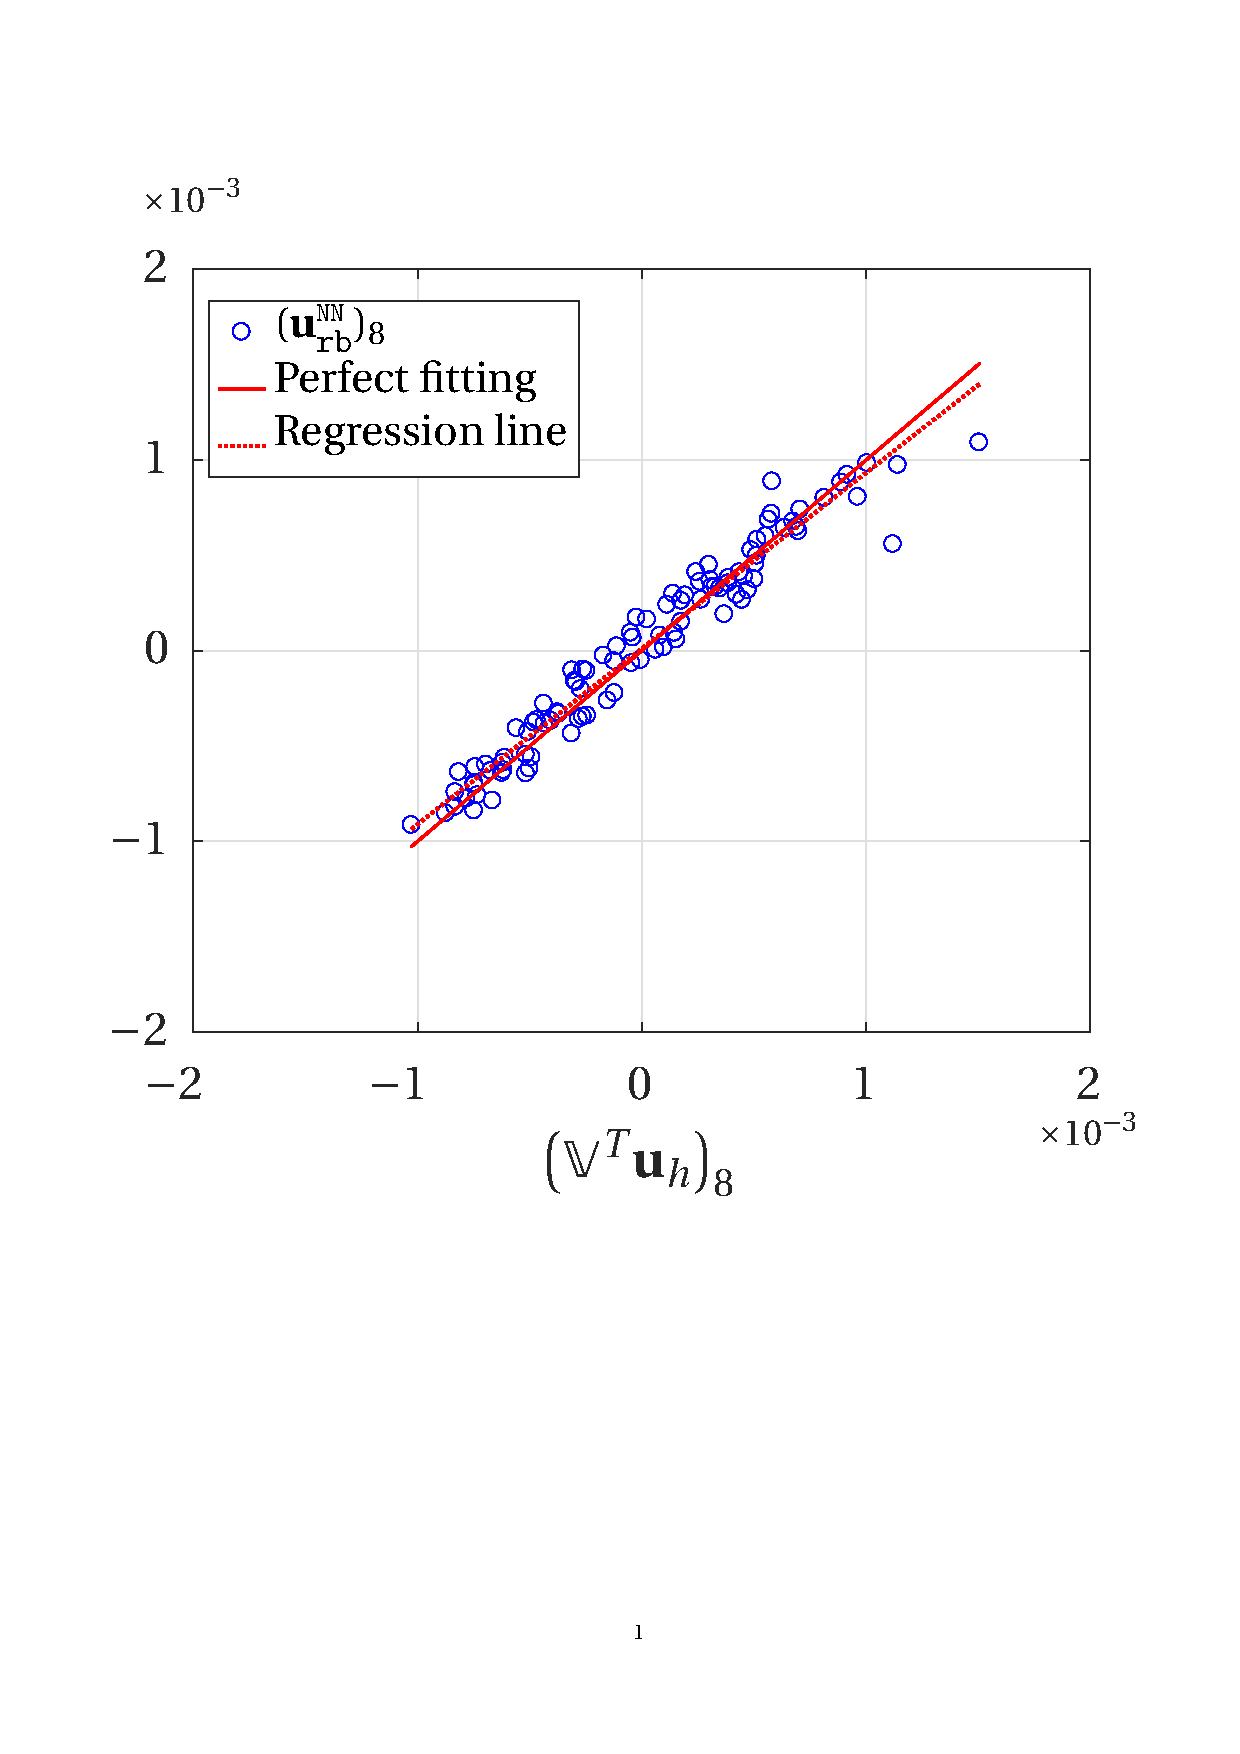
\includegraphics[scale = 0.4, trim = {0cm 9cm 1cm 1cm}, clip]{poisson1d_2_regression_8}}
			\subfloat{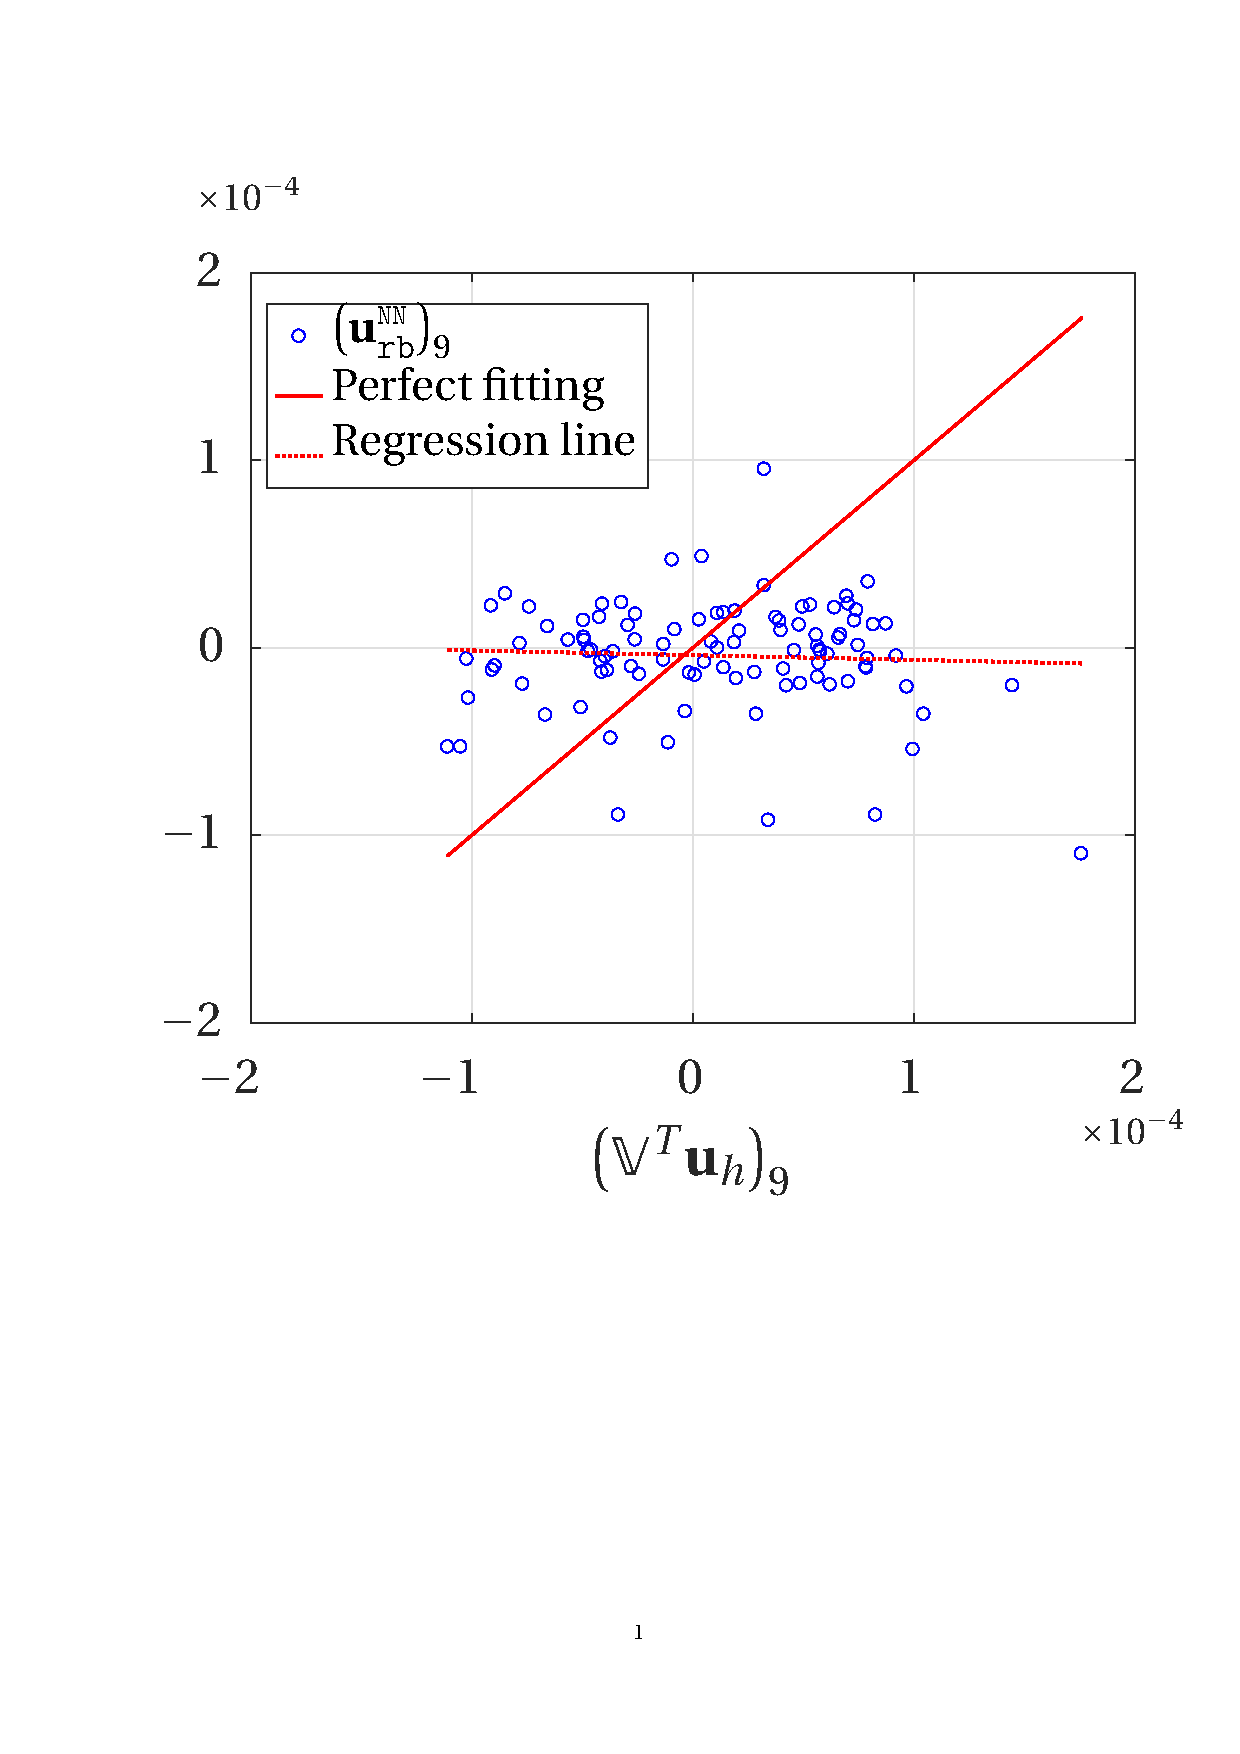
\includegraphics[scale = 0.4, trim = {1cm 9cm 1cm 1cm}, clip]{poisson1d_2_regression_9}}
			
			\caption{From left to right, top to bottom: regression plots for the first, seventh, eighth and nine scalar components of the outputs provided on $\Xi_{te}$ by a network with $H_1 = H_2 = 25$ neurons per hidden layer, trained to approximate the map \eqref{eq:map-to-approximate} for problem \eqref{eq:poisson1d-2}.}
			\label{fig:poisson1d-2-fig3}
		\end{figure}
			
	\subsection{Nonlinear test case, three parameters}
	\label{section:poisson1d-3}
	
		The last problem we consider for the one-dimensional Poisson equation features an exponential nonlinearity (in the diffusion coefficient) and involves three parameters:
		\begin{equation}
			\label{eq:poisson1d-3}
			\begin{cases}
				& - \big( \exp(u(\bg{\mu})) ~ u(\bg{\mu})' \big)' = s(x; \, \bg{\mu}) \hspace*{0.3cm} \text{in $\Omega = \left( -\dfrac{\pi}{2}, \, \dfrac{\pi}{2} \right)$} \, , \\[0.3cm]
				& u(\bg{\mu}) \big|_{x = \pm \nicefrac{\pi}{2}} = \mu_2 \left( 2 \pm \sin\left( \dfrac{\mu_1 \, \pi}{2} \right) \right) \exp \left( \pm \dfrac{\mu_3 \, \pi}{2} \right) \, ,
			\end{cases}
		\end{equation}
		with $\bg{\mu} = \big(\mu_1, \, \mu_2, \, \mu_3 \big) \in \mathcal{P} = \big[ 1, \, 3 \big] \times \big[ 1, \, 3 \big] \times \big[ -0.5, \, 0.5 \big]$ and $s(\cdot; \bg{\mu})$ such that \[ u_{ex}(x; \, \bg{\mu}) = \mu_2 \big( 2 + \sin(\mu_1 \, x) \big) \, \exp \big( \mu_3 \, x \big) \] is the exact solution to the problem for any $\bg{\mu} \in \mathcal{P}$. Figure \ref{fig:poisson1d-3-fig1} represents the first $10$ POD modes for the problem, yielded by singular value decomposition of an ensemble of $N = 100$ (linear) FE snapshots computed over a uniform grid consisting of $100$ nodes. Their inclusion within the standard POD-Galerkin RB framework enables an average relative error of about $10^{-5}$ on a test set $\Xi_{te}$ of $N_{te} = 100$ randomly chosen samples. This is whitnessed by Fig. \ref{fig:poisson1d-3-fig2}, offering a convergence analysis with respect to the number of basis functions retained in the model (\emph{left}). The results for the POD-NN method, employing three-layers neural networks with a varying number of neurons and learning patterns, are provided as well, together with a comparison with the FE solution for some parameter values (\emph{right}). Note that, when only a few modes are considered (say $L \leq 5)$, the proposed reduced basis scheme may lead to a significant reduction of the error with respect to the POD-G technique. Moreover, as we expand the training set, we get more accurate predictions for a larger number of POD coefficients, provided that we allow the size of the network to increase. 
		
		\vspace*{-0.15cm}
		
		\begin{figure}[H]
			\center
			\subfloat[$\psi_1$]{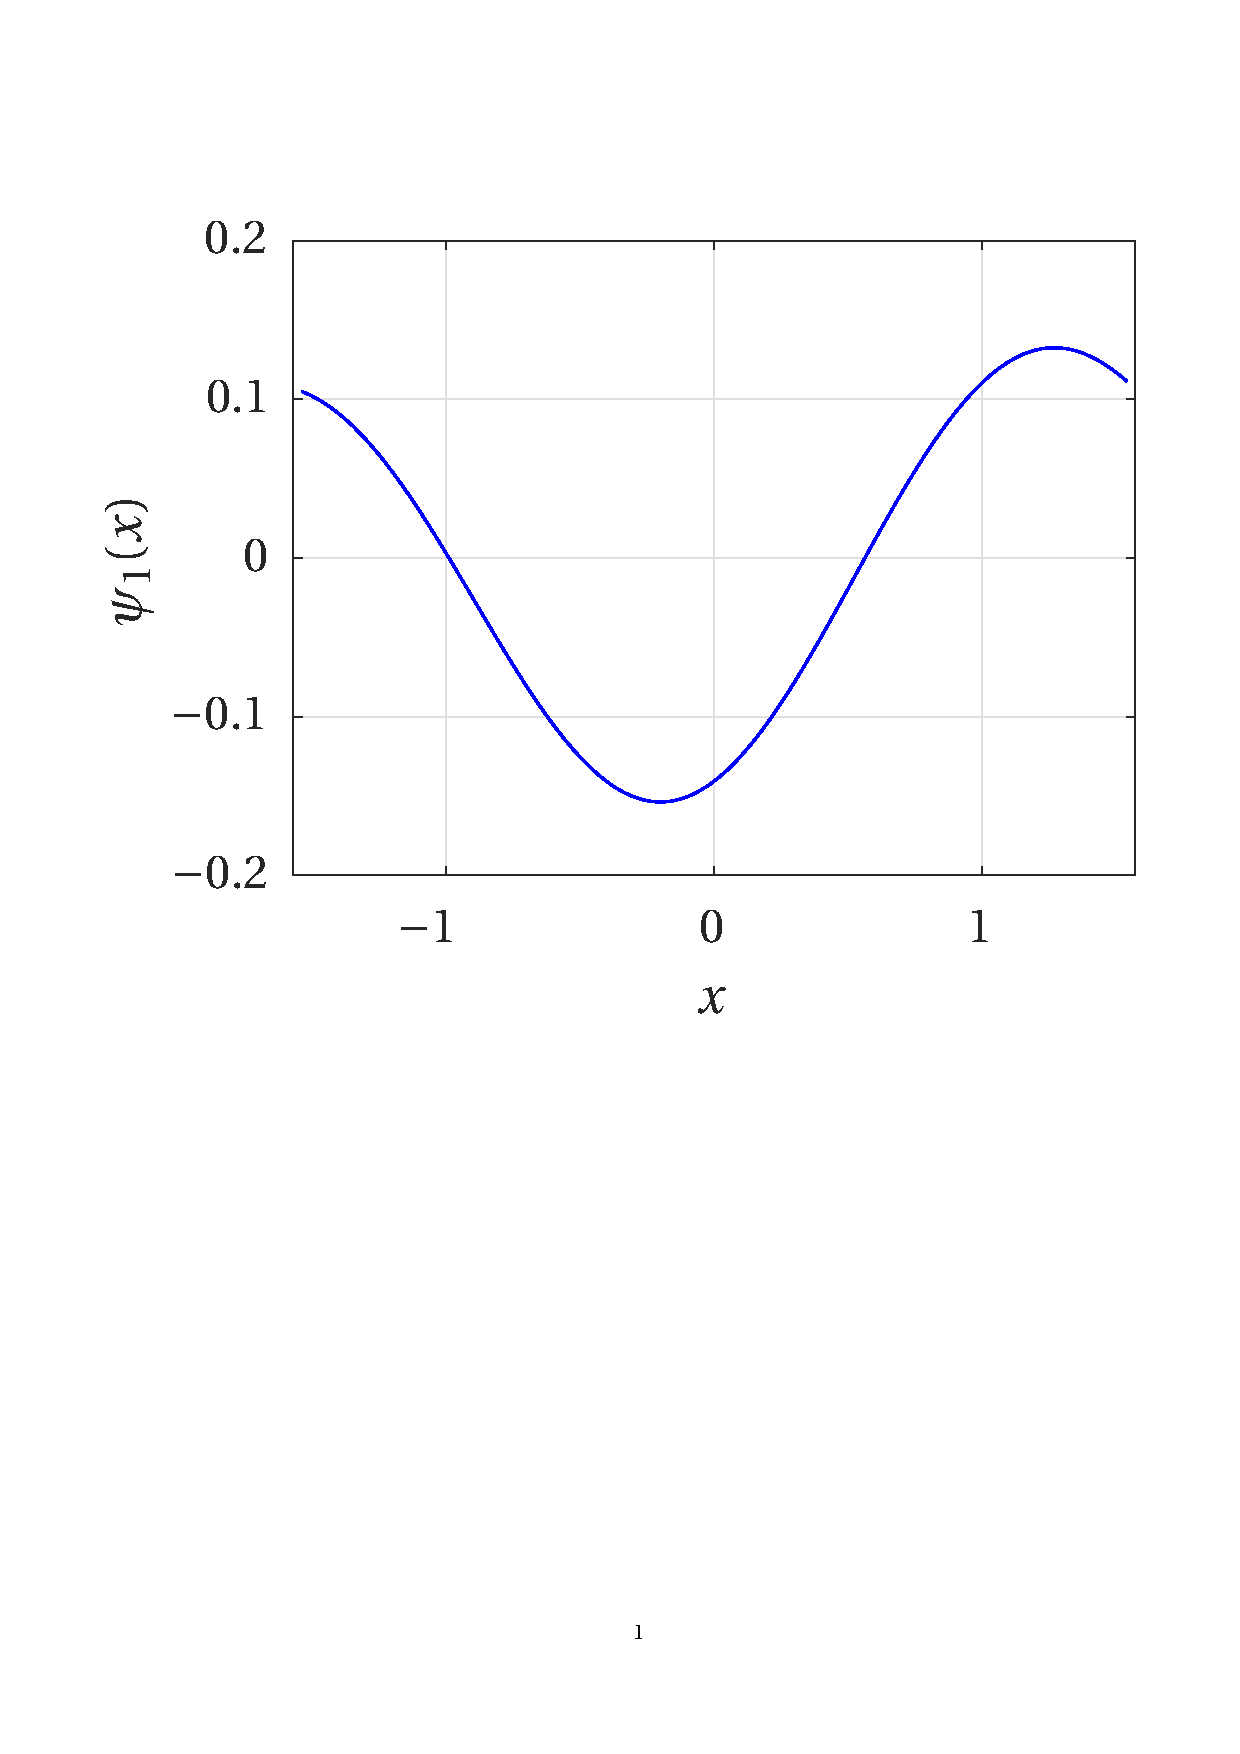
\includegraphics[scale = 0.185, trim = {2.75cm 12cm 1.5cm 4cm}, clip]{poisson1d_3_basis1}}
			\subfloat[$\psi_2$]{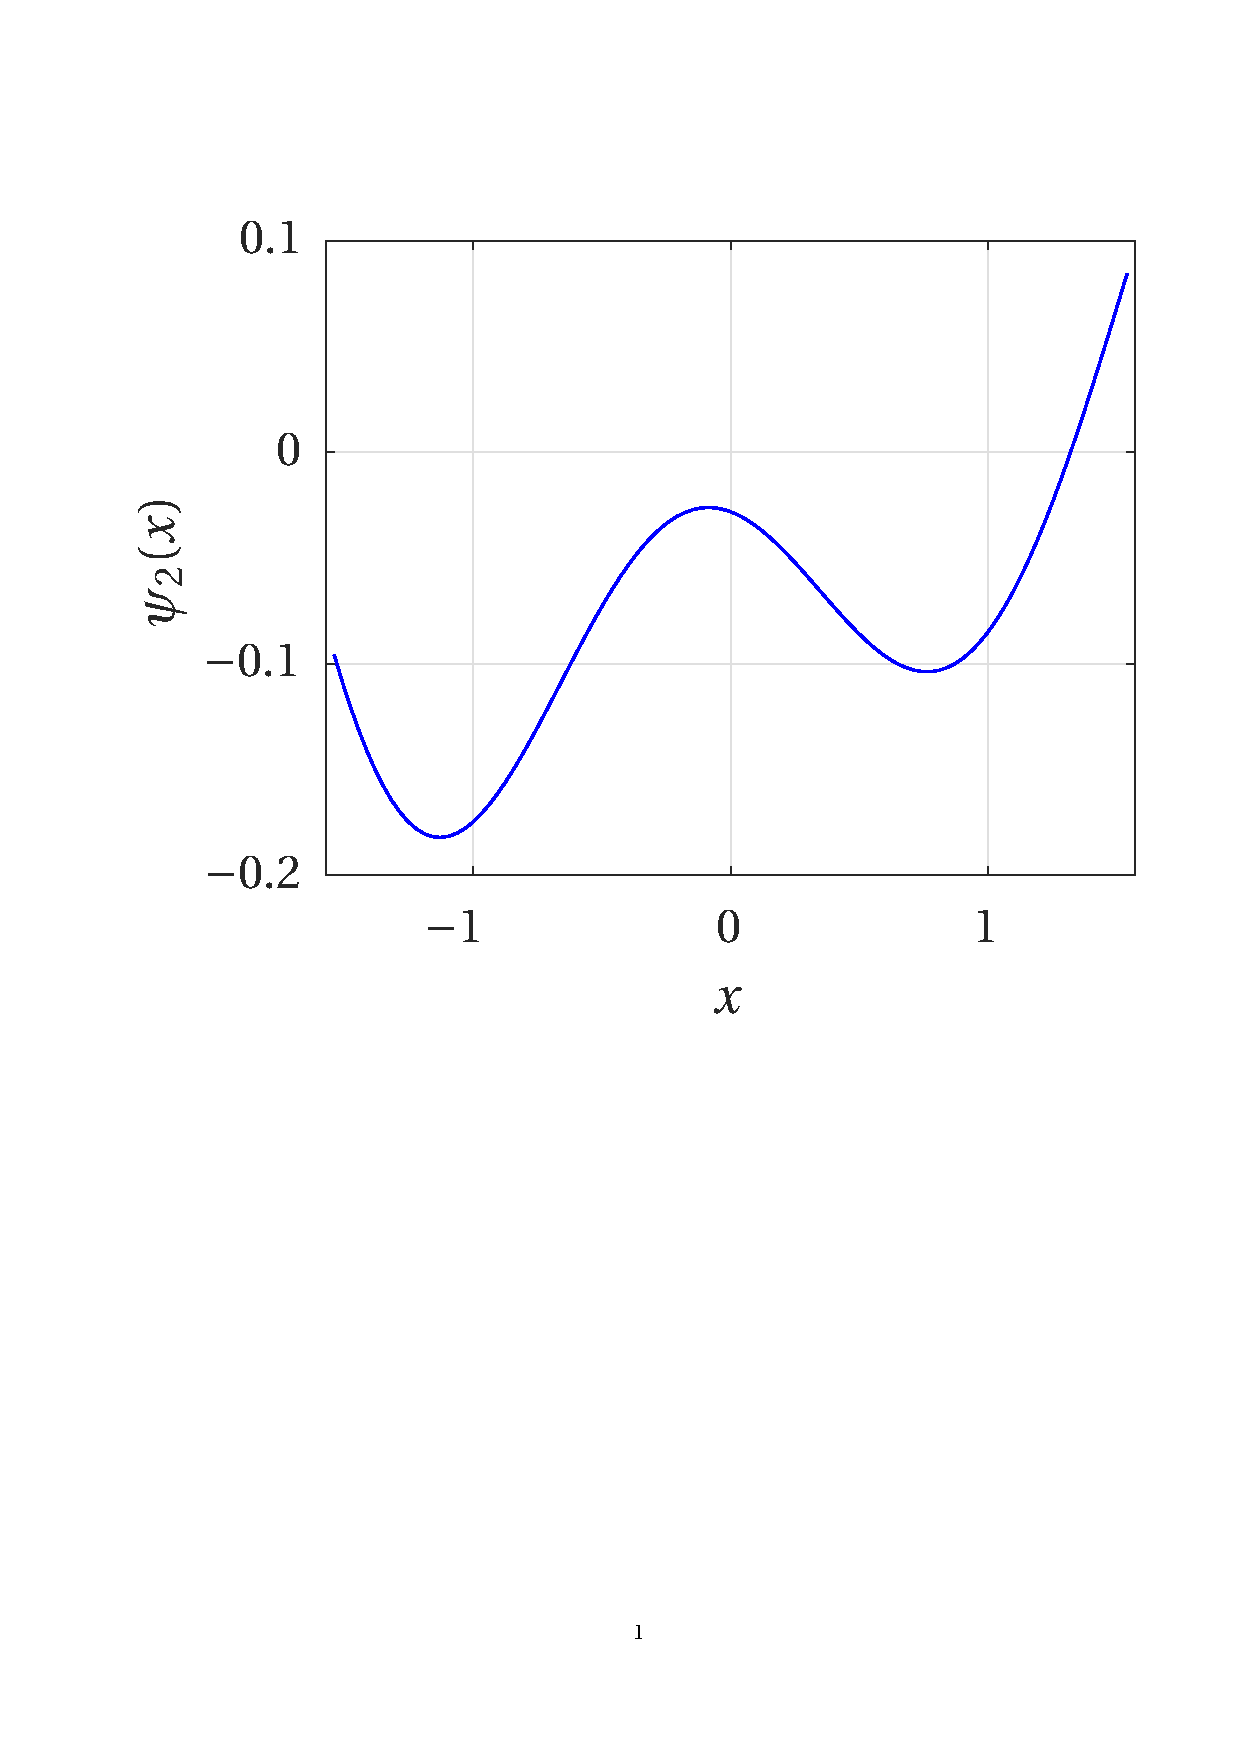
\includegraphics[scale = 0.185, trim = {3.25cm 12cm 1.5cm 4cm}, clip]{poisson1d_3_basis2}}
			\subfloat[$\psi_3$]{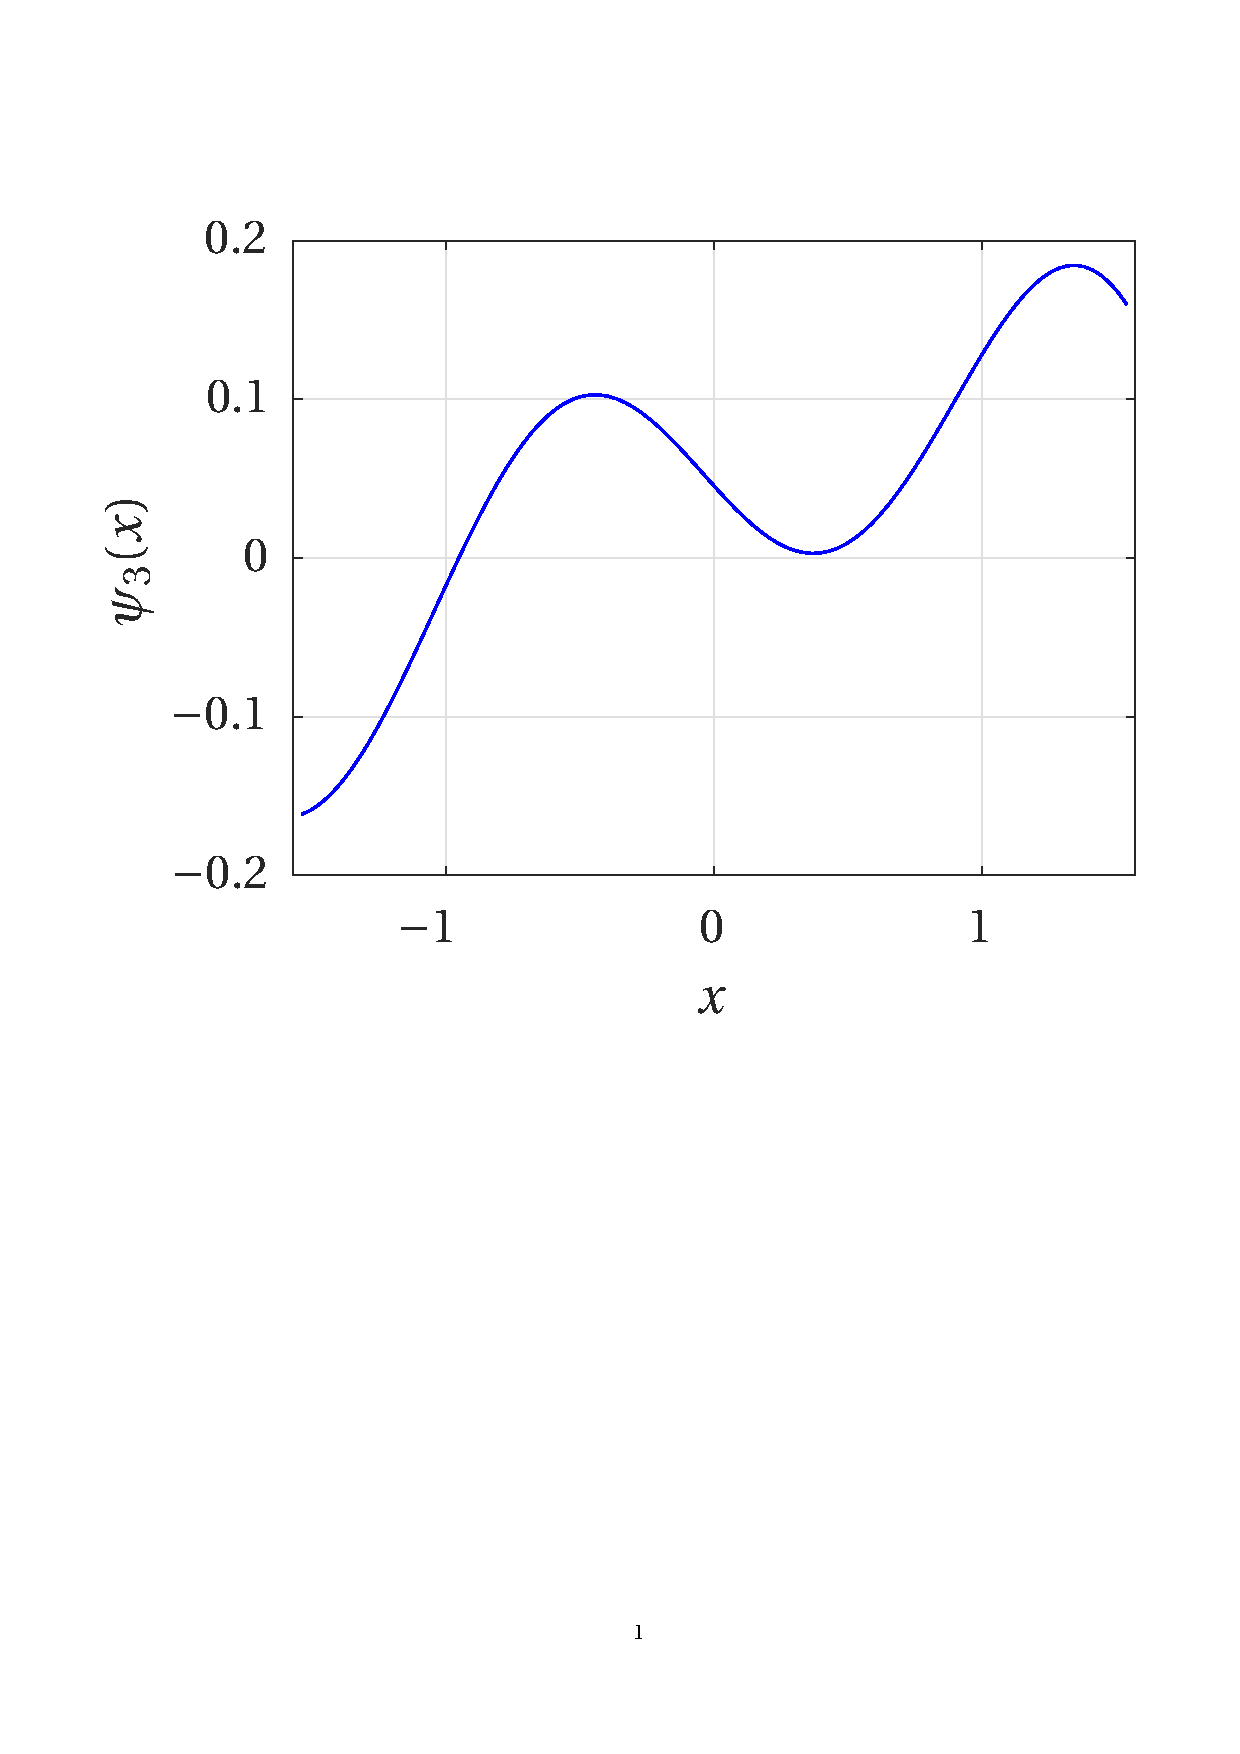
\includegraphics[scale = 0.185, trim = {2.75cm 12cm 1.5cm 4cm}, clip]{poisson1d_3_basis3}}
			\subfloat[$\psi_4$]{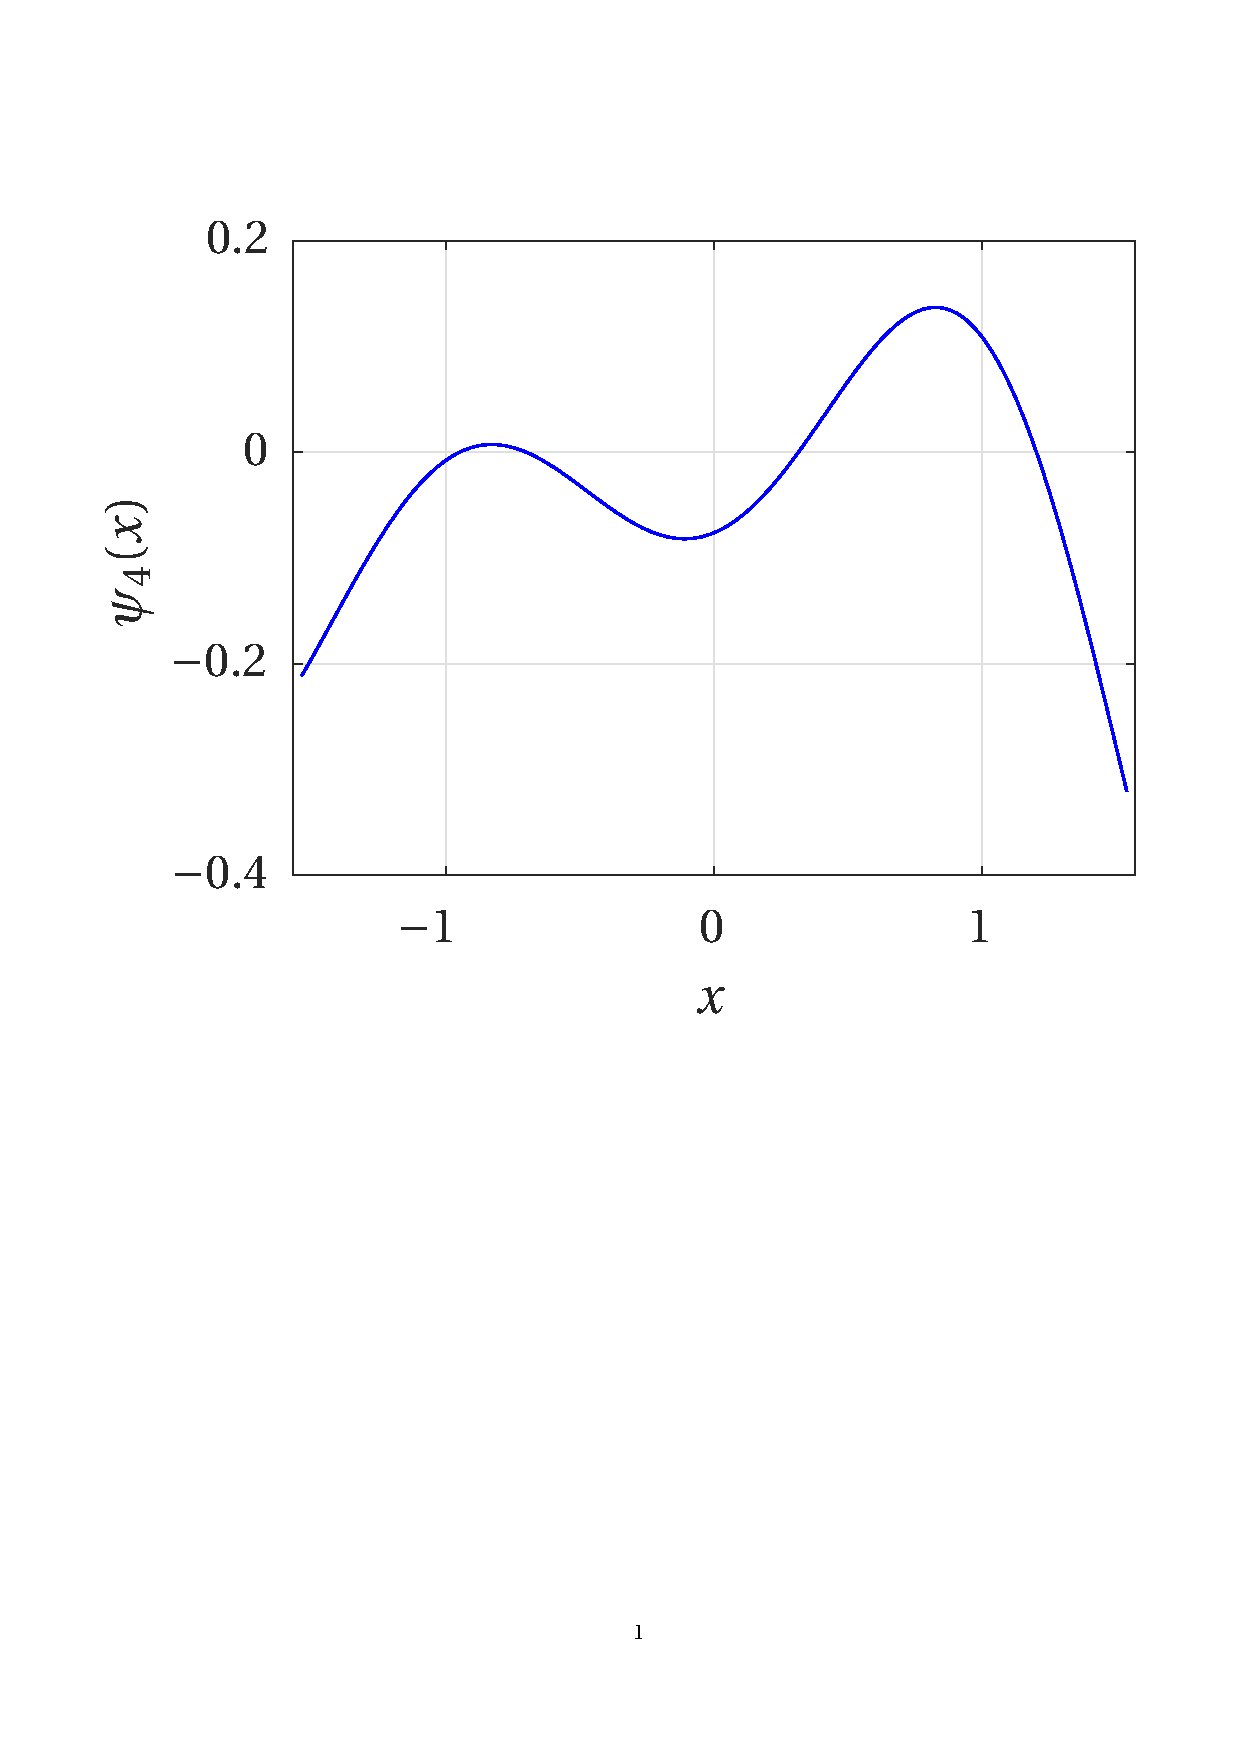
\includegraphics[scale = 0.185, trim = {2.75cm 12cm 1.5cm 4cm}, clip]{poisson1d_3_basis4}}
			\subfloat[$\psi_5$]{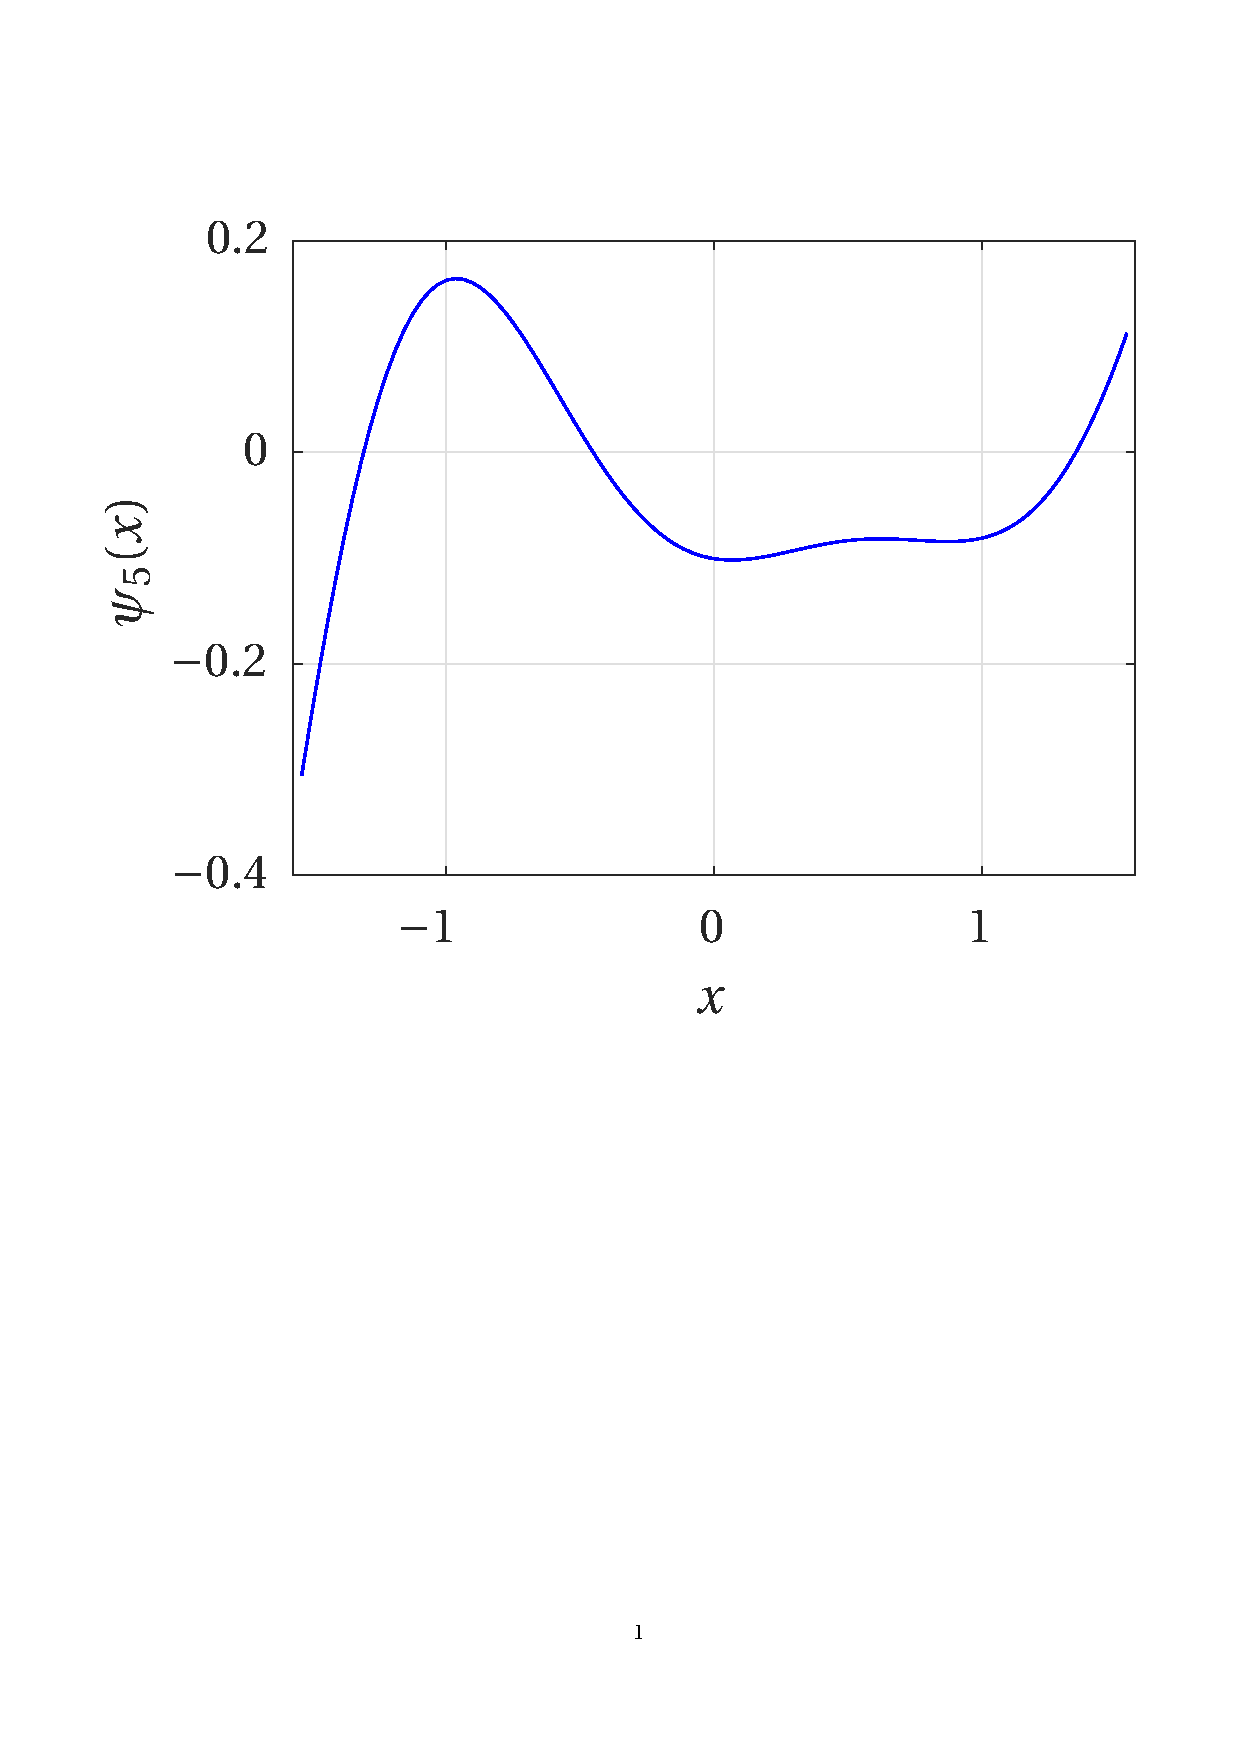
\includegraphics[scale = 0.185, trim = {2.75cm 12cm 1.5cm 4cm}, clip]{poisson1d_3_basis5}} \\[-0.25cm]
			\subfloat[$\psi_6$]{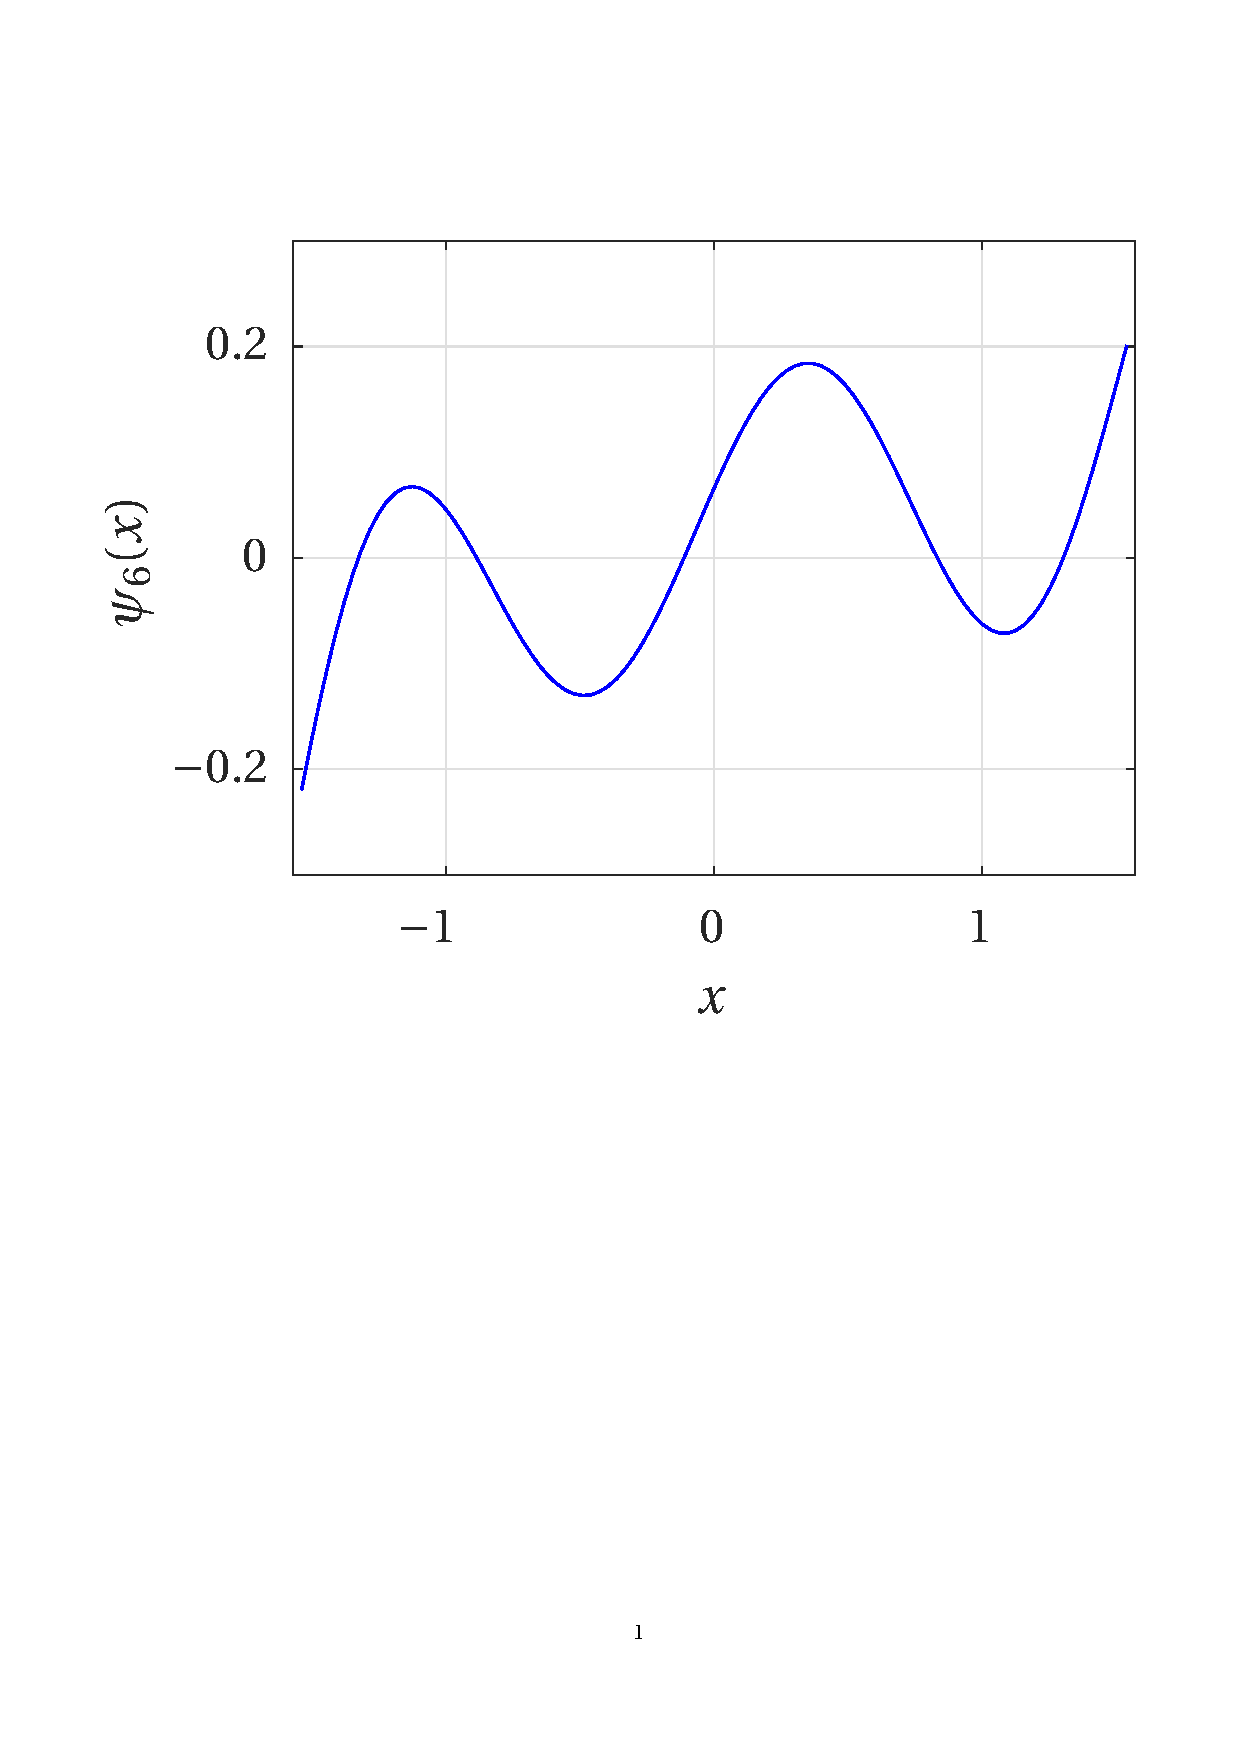
\includegraphics[scale = 0.185, trim = {2.75cm 12cm 1.5cm 1cm}, clip]{poisson1d_3_basis6}}
			\subfloat[$\psi_7$]{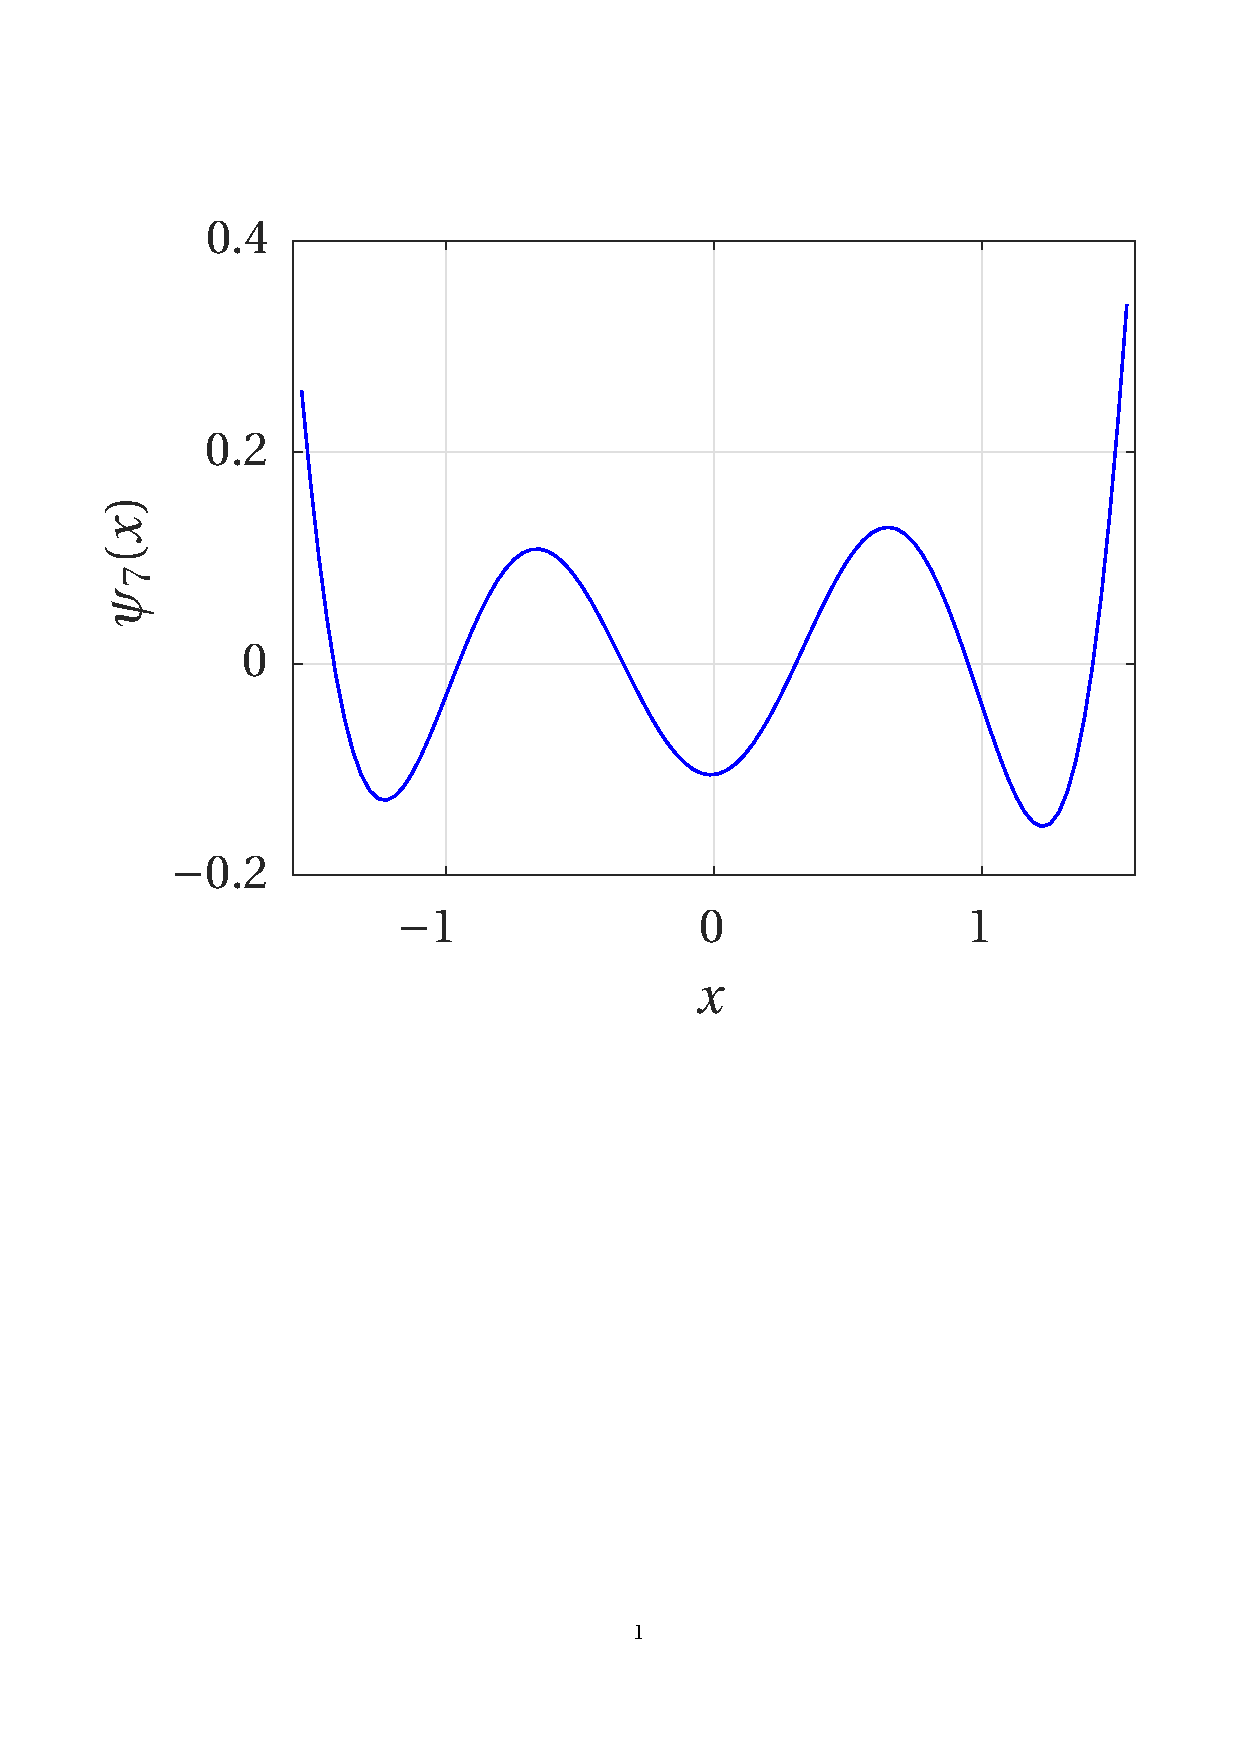
\includegraphics[scale = 0.185, trim = {2.75cm 12cm 1.5cm 1cm}, clip]{poisson1d_3_basis7}}
			\subfloat[$\psi_8$]{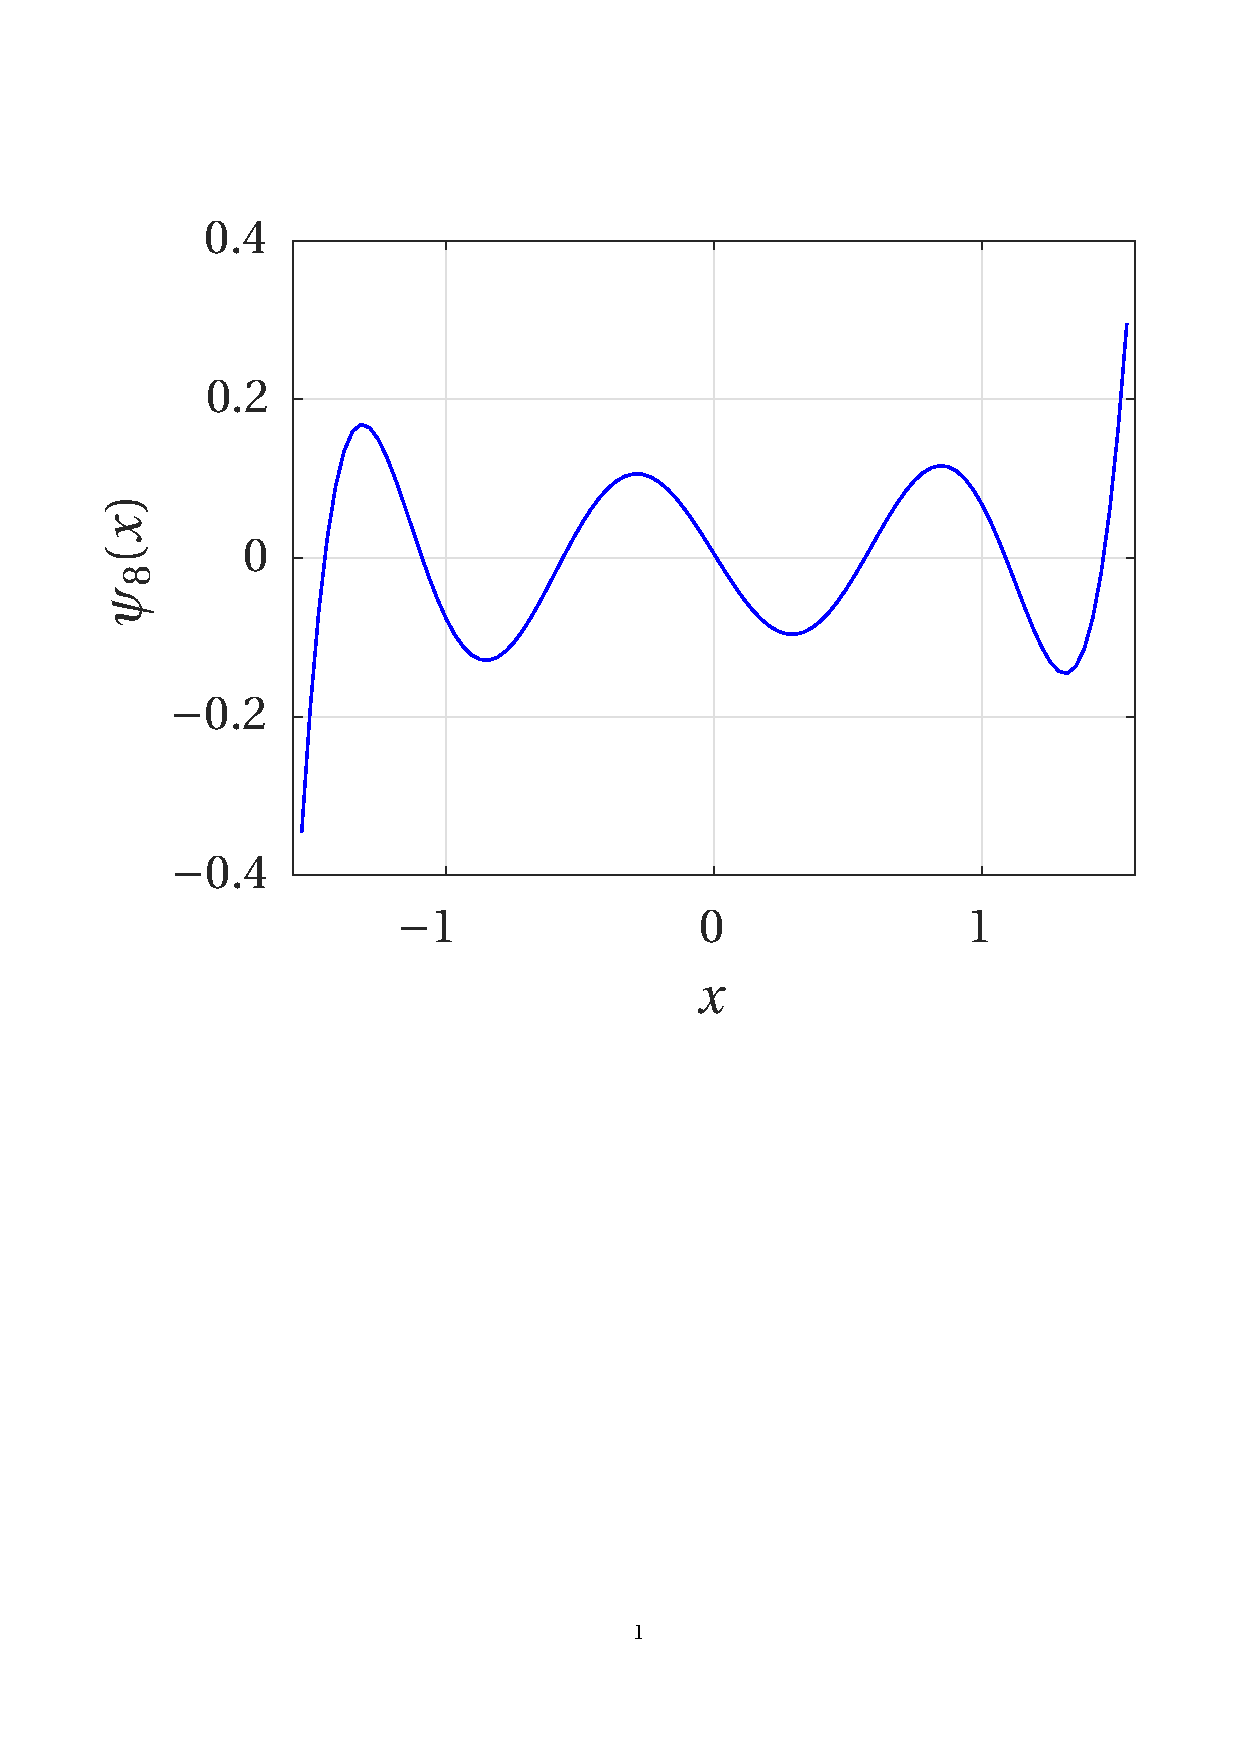
\includegraphics[scale = 0.185, trim = {2.75cm 12cm 1.5cm 1cm}, clip]{poisson1d_3_basis8}}
			\subfloat[$\psi_9$]{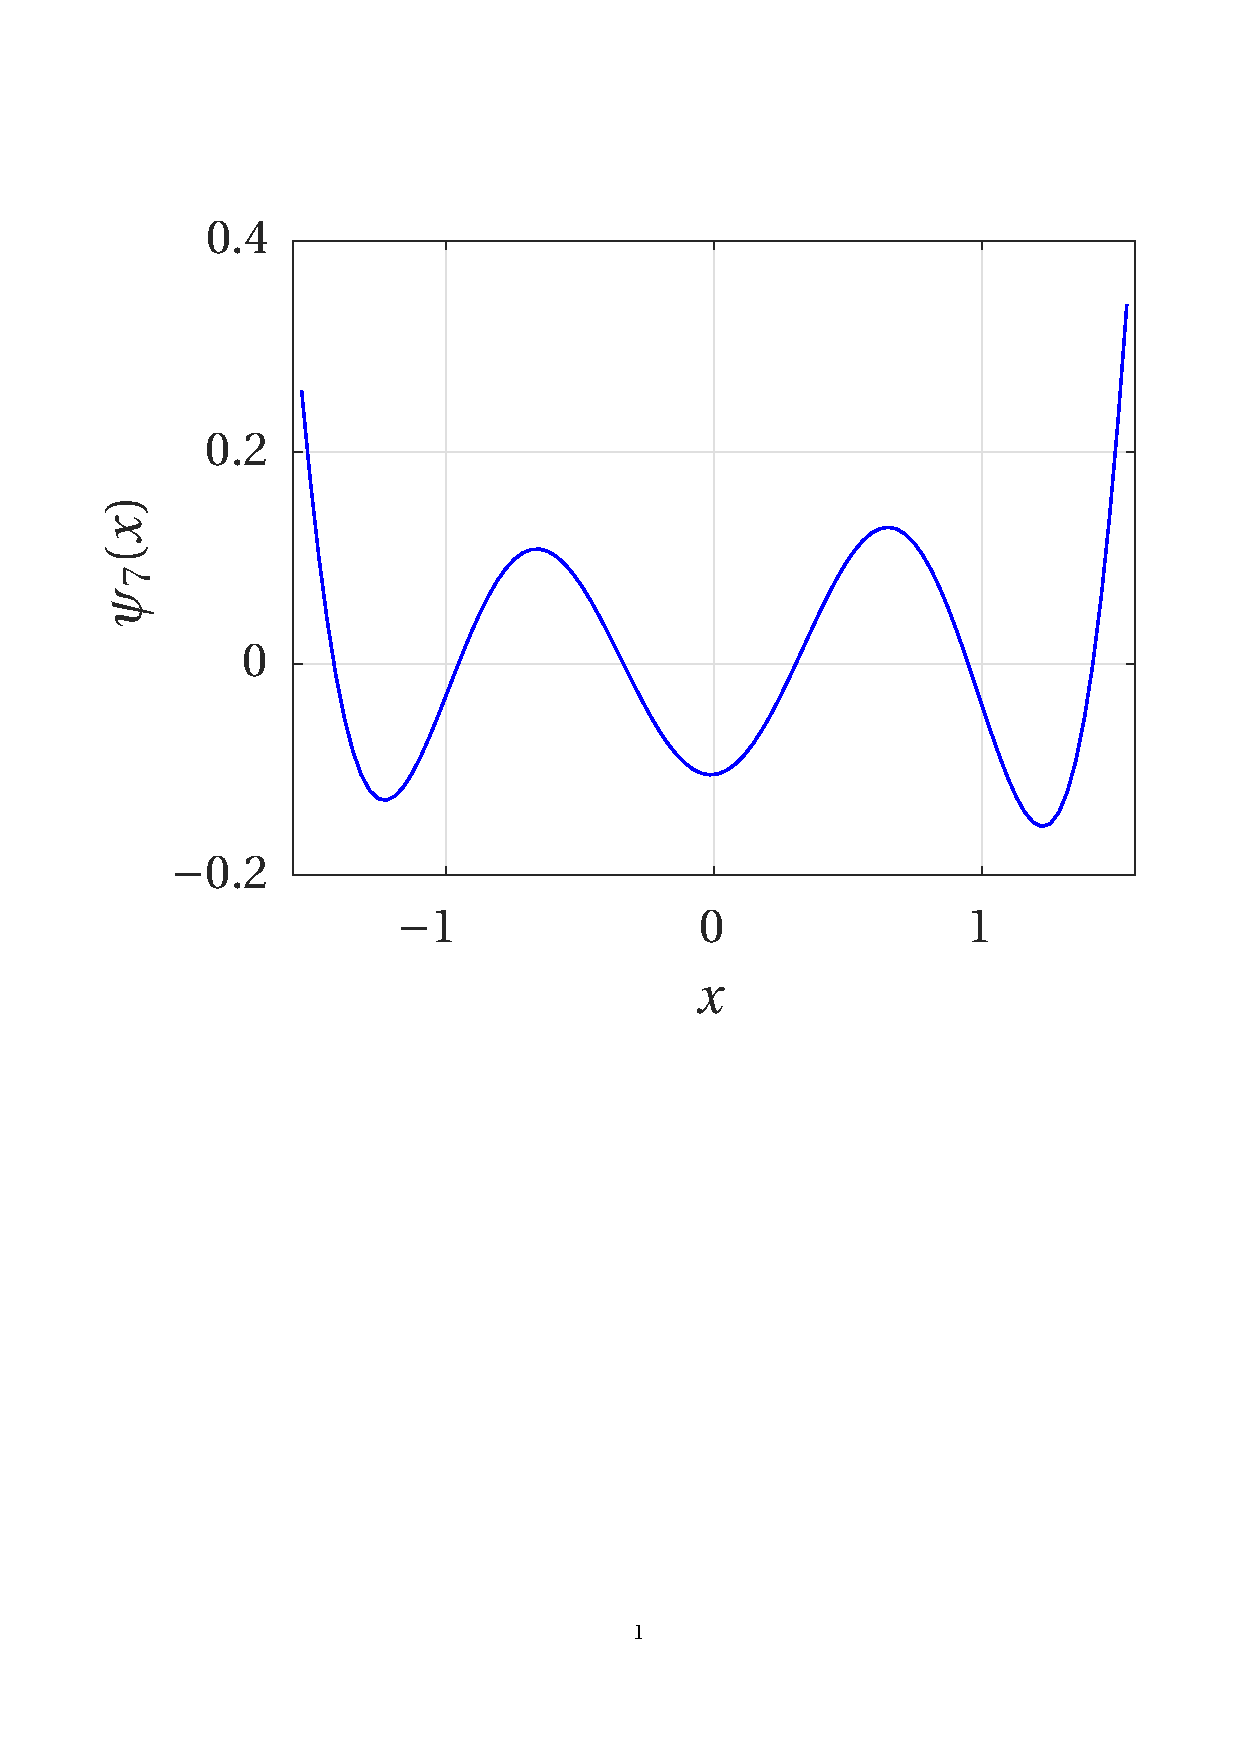
\includegraphics[scale = 0.185, trim = {2.75cm 12cm 1.5cm 1cm}, clip]{poisson1d_3_basis9}}
			\subfloat[$\psi_{10}$]{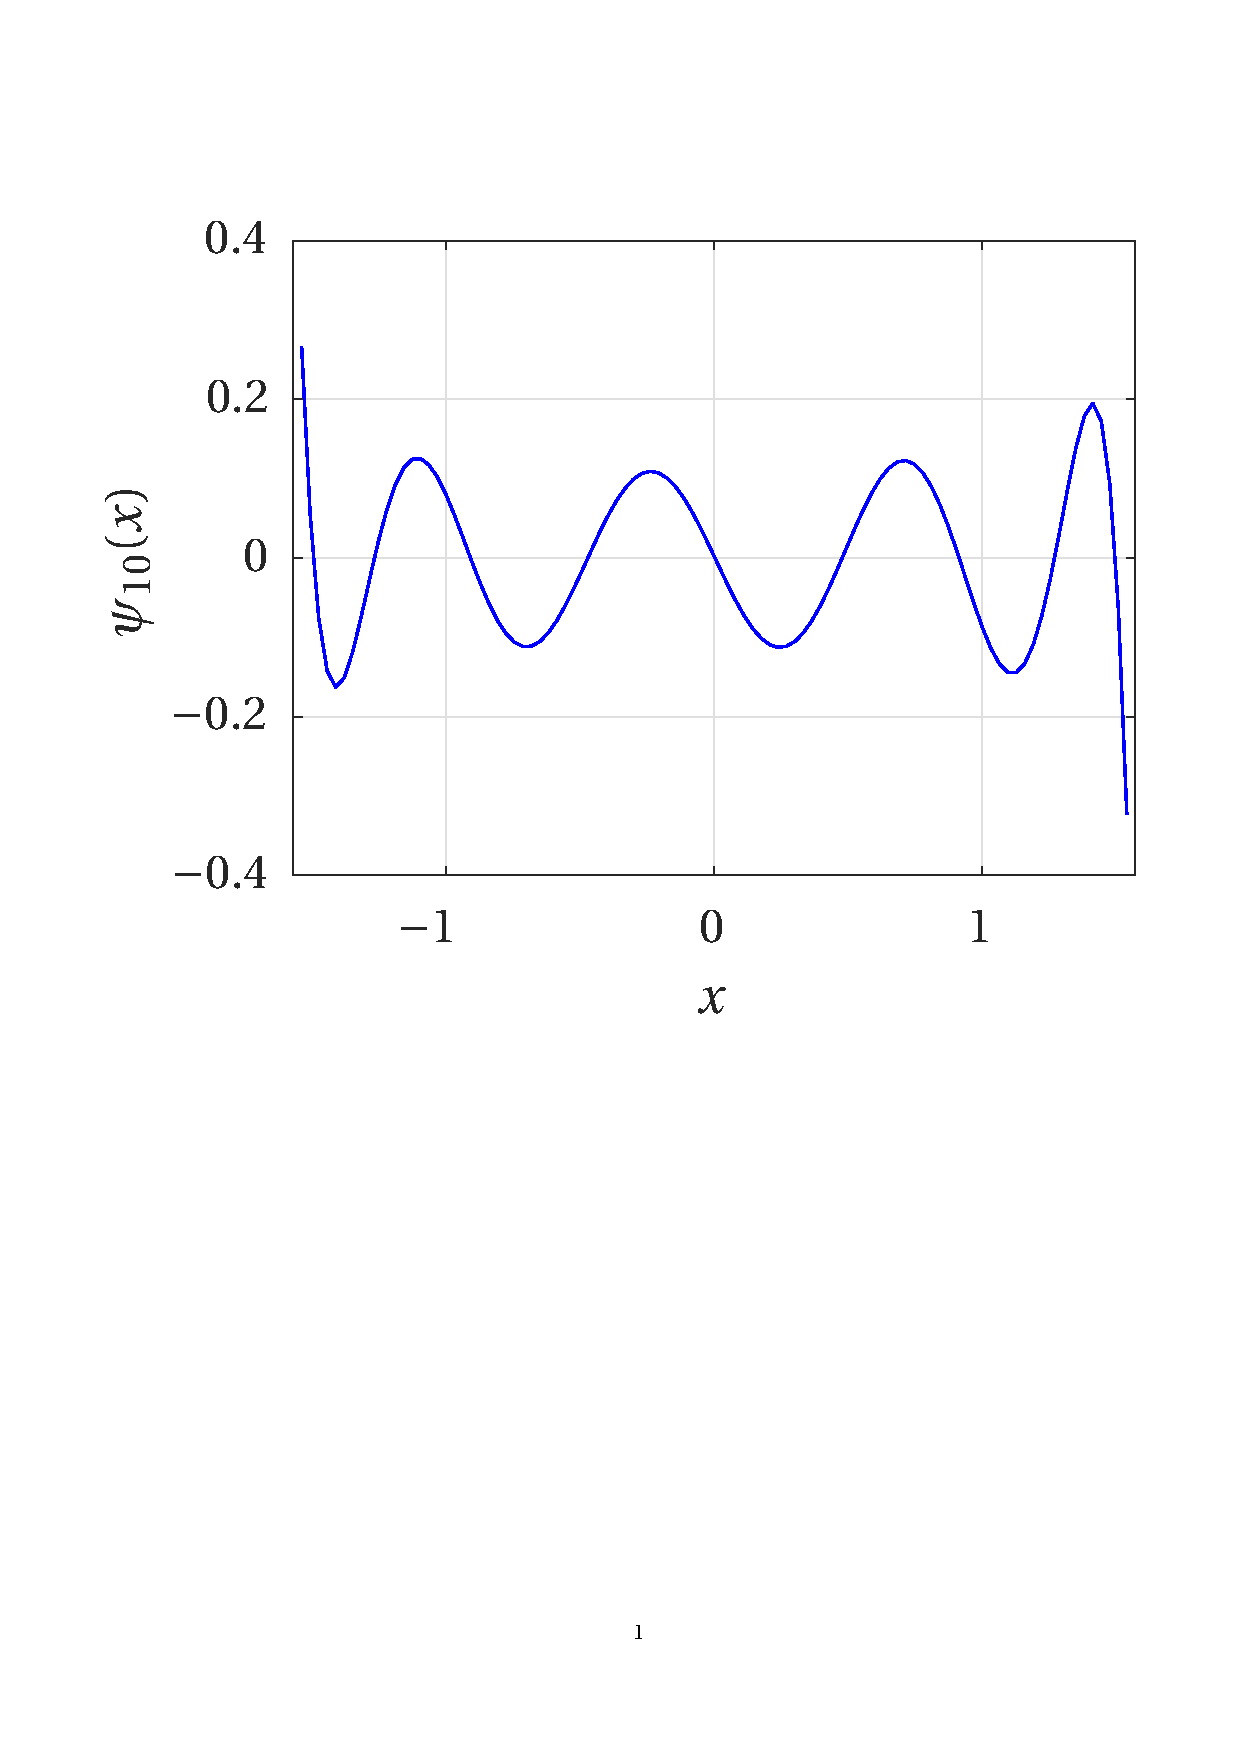
\includegraphics[scale = 0.185, trim = {2.75cm 12cm 1.5cm 1cm}, clip]{poisson1d_3_basis10}}
			
			\caption{The first $10$ POD basis functions for the (nonlinear) Poisson problem \eqref{eq:poisson1d-3}.}
			\label{fig:poisson1d-3-fig1}
		\end{figure}
		
		\vspace*{-0.4cm}
		
		\begin{figure}[H]
			\center
			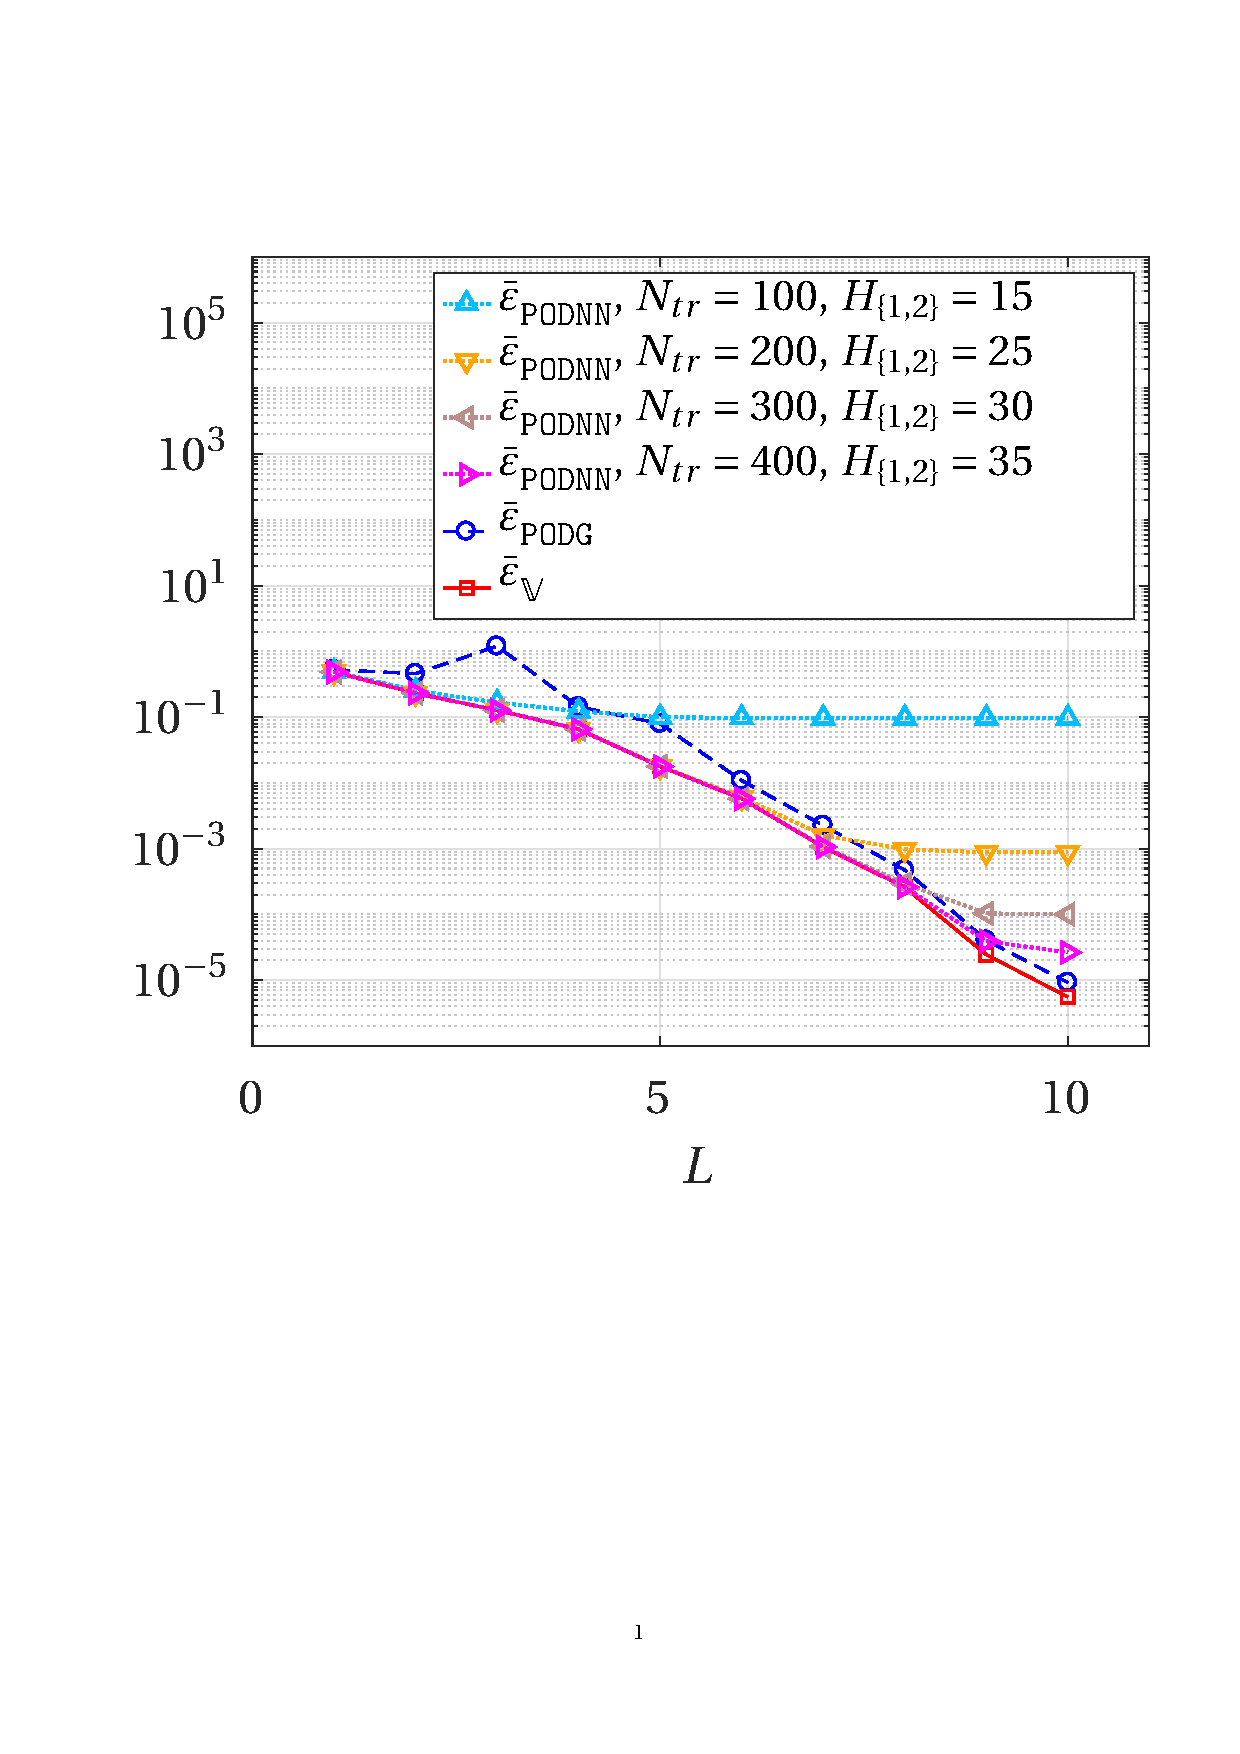
\includegraphics[scale = 0.4, trim = {1cm 9cm 1cm 3cm}, clip]{poisson1d_3_error_vs_rank}
			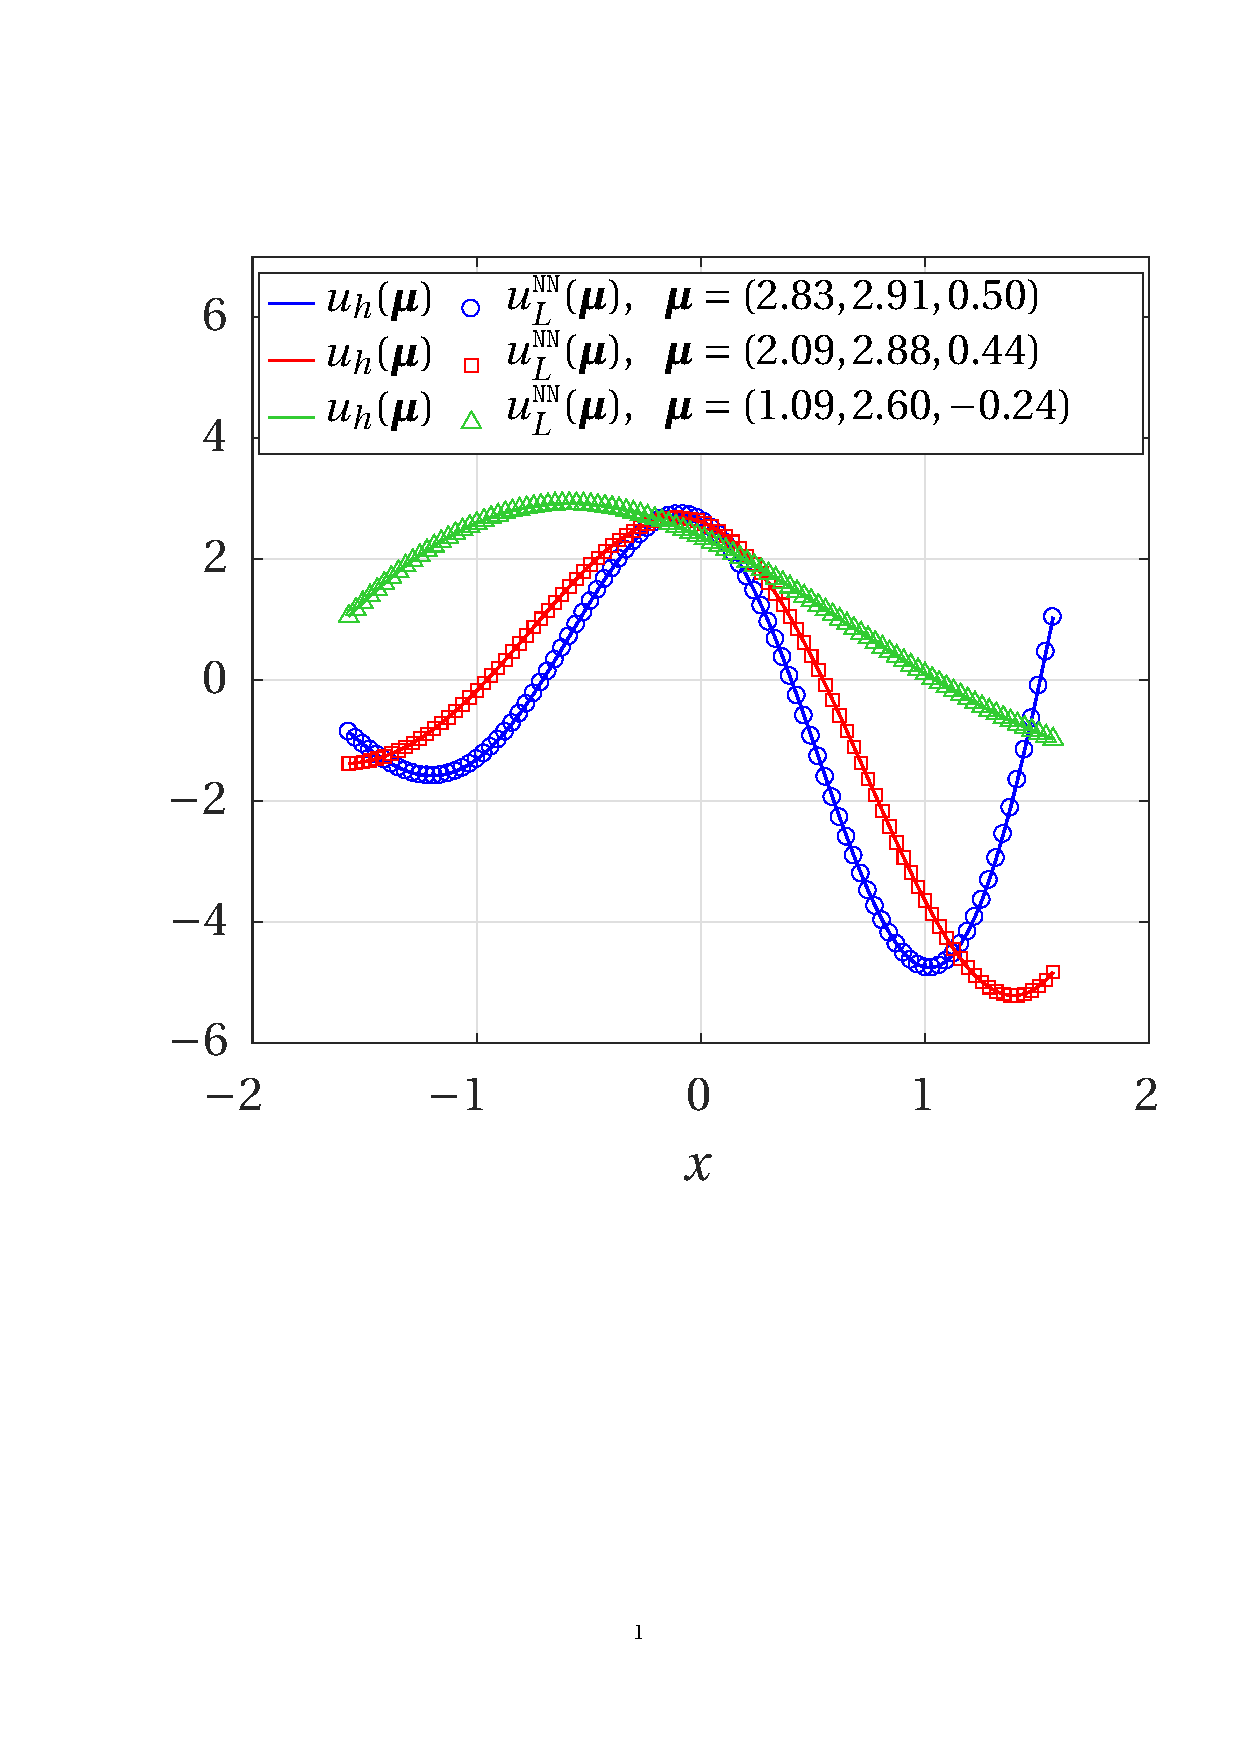
\includegraphics[scale = 0.4, trim = {1.5cm 9cm 1.5cm 3cm}, clip]{poisson1d_3_fe_vs_podnn}
			
			\caption{Convergence analysis for the POD-G and POD-NN methods applied to problem \eqref{eq:poisson1d-3} (\emph{left}) and comparison between the FE and the POD-NN solutions for three parameter values (\emph{right}). These latter results have been obtained via a neural network with $H_1 = H_2 = 35$ units per hidden layer, and considering $L = 10$ POD modes.}
			\label{fig:poisson1d-3-fig2}
		\end{figure}
		
		Concerning the results shown in the left plot of Fig. \ref{fig:poisson1d-3-fig2}, we should point out an important remark, valid throughout the chapter. The results refer to neural networks trained via exposition to the set of coefficients \[ \big\lbrace \big( u_h(\bg{\mu}), \, \psi_i \big)_h \big\rbrace_{i = 1}^{\scriptscriptstyle{\bar{L}}} \equiv \big\lbrace \big( \mathbf{u}_h(\bg{\mu}), \, \bg{\psi}_i \big)_{\mathbb{R}^M} \big\rbrace_{i = 1}^{\scriptscriptstyle{\bar{L}}} \] for each learning sample $\bg{\mu} \in \Xi_{tr}$, with $\bar{L} = 10$. Therefore, each network is equipped with $\bar{L} = 10$ output neurons - one for each coefficient. Once the training has been successfully completed, given a new input $\bg{\mu} \in \mathcal{P}$, the corresponding POD-NN RB solution of order $\bar{L}$ is obtained as:
		\begin{equation}
			\label{eq:podnn-solution-full}
			\mathbf{u}_{\bar{L}}^{\texttt{NN}}(\bg{\mu}) = \sum_{i = 1}^{\bar{L}} \big( \mathbf{u}_{\bar{L}}^{\texttt{NN}} \big)_i \bg{\psi}_i \, ,
		\end{equation} 
		where $\big( \mathbf{u}_{\bar{L}}^{\texttt{NN}} \big)_i$ denotes the network response observed at the $i$-th output neuron, $i = 1, \, \ldots \, , \bar{L}$. Although $\mathbf{u}_{\bar{L}}^{\texttt{NN}}(\bg{\mu})$ represents the best prediction for $\mathbf{u}_h(\bg{\mu})$ provided by the network, we can as well construct lower-ordered approximations $\mathbf{u}_L^{\texttt{NN}}(\bg{\mu})$, with $L < \bar{L}$, by simply retaining the first $L$ terms in the summation \eqref{eq:podnn-solution-full}. The claim is that such $L$-order RB solution is basically as accurate as the one we could obtain by exposing the network to exactly $L$ POD coefficients per training sample. In other terms, employing a larger amount of modes during the training than in the subsequent online queries, so somehow offering the network a wider overview on the problem, does not enable a substantial improvement in the performace. A confirmation of this is given by Fig. \ref{fig:poisson1d-3-fig3}, reporting the average relative POD-NN error $\bar{\varepsilon}_{\texttt{NN}}^{}(L)$, for $1 \leq L \leq 10$, yielded by networks equipped with either $20$ or $35$ units per hidden layer, and exposed, within the learning phase, to $N_{tr} = 300$ samples and either $L$ or $\bar{L}$ expansion coefficients per sample.
		
		\begin{figure}[H]
			\center
			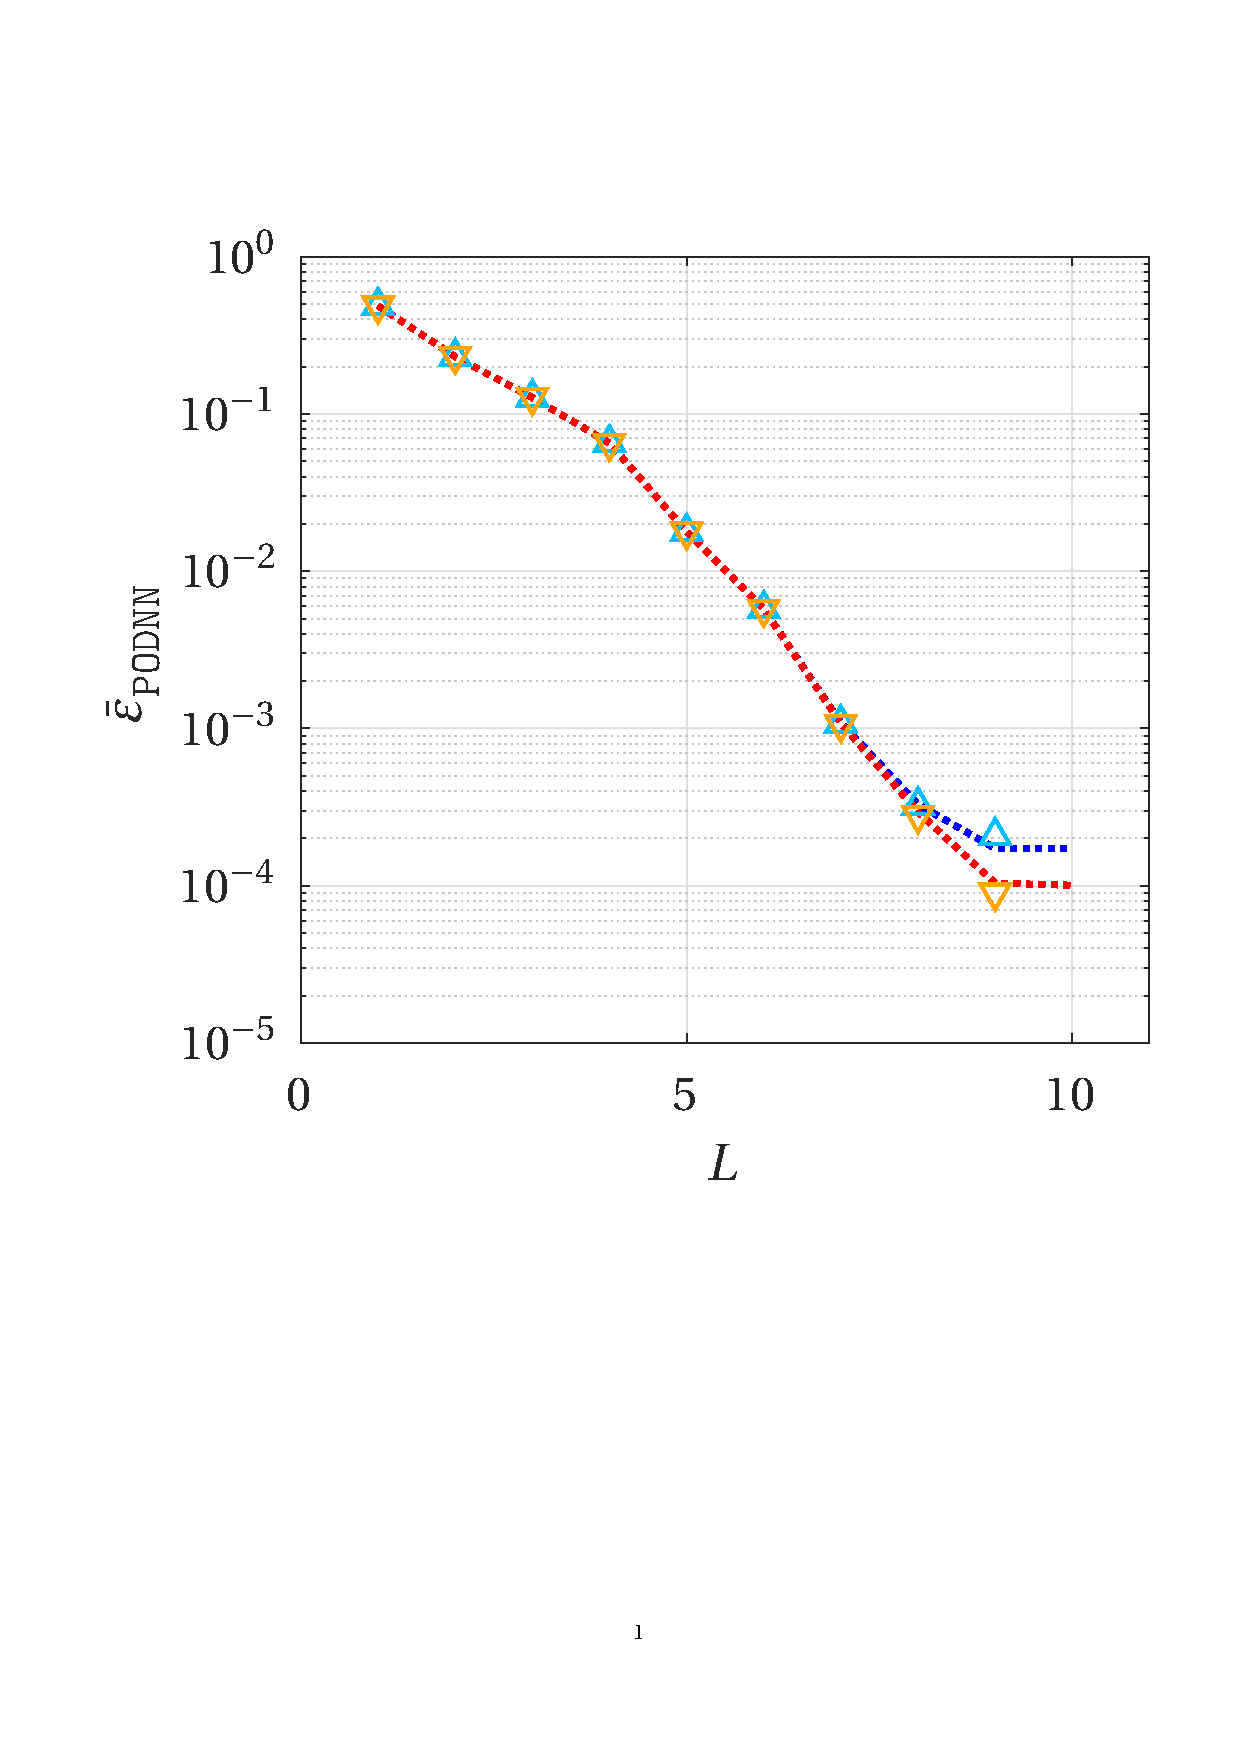
\includegraphics[scale = 0.40, trim = {1cm 9cm 1cm 3cm}, clip]{poisson1d_3_nn_test}
			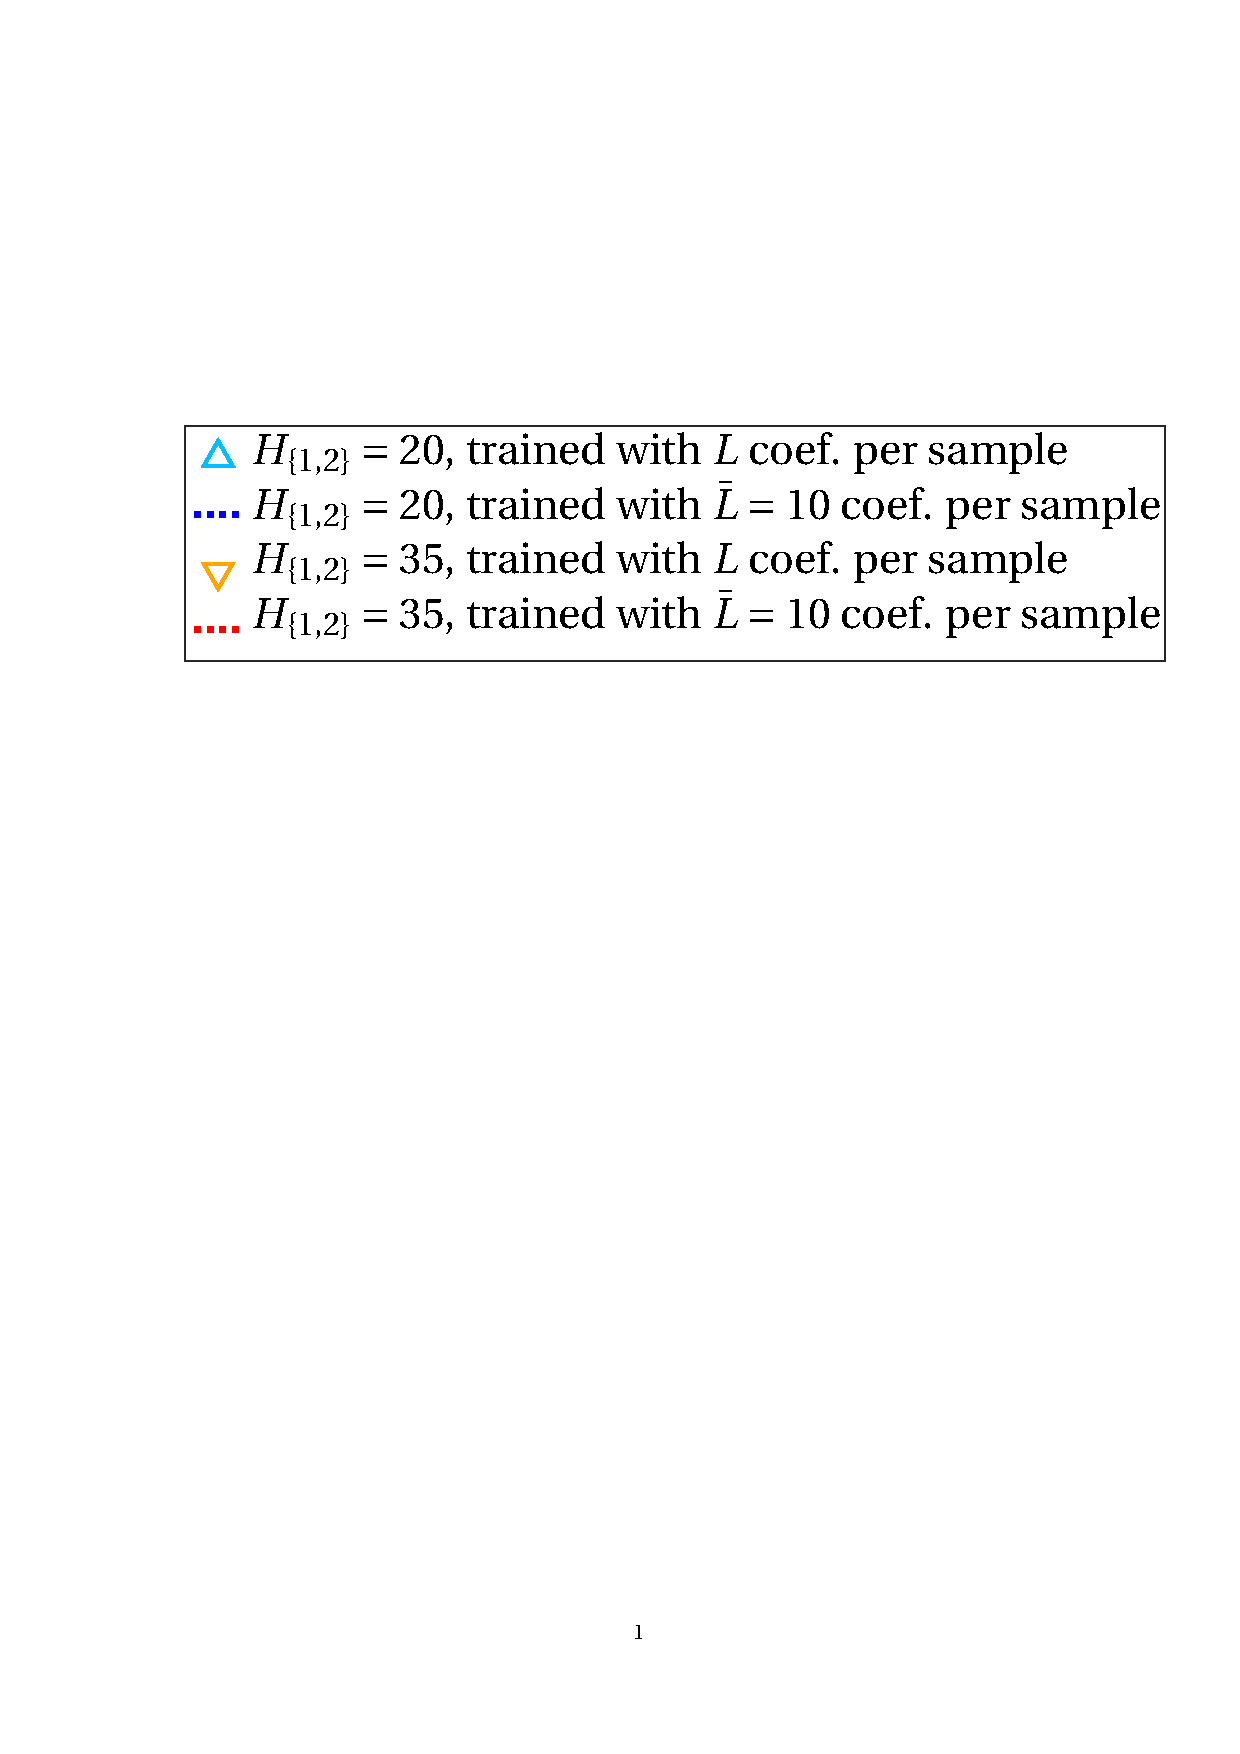
\includegraphics[scale = 0.42, trim = {2cm 11.25cm 1cm 3cm}, clip]{poisson1d_3_nn_test_legend}
			
			\caption{Sensitivity analysis for the POD-NN method applied to problem \eqref{eq:poisson1d-3} with respect to the number of POD coefficients (per sample) used during the training; to prevent overfitting, $N_{tr} = 300$ learning patterns have been used.}
			\label{fig:poisson1d-3-fig3}
		\end{figure}
		
	\clearpage
					
	\section{Two-dimensional Poisson equation}
	\label{section:Two-dimensional Poisson equation (results)}
	
		As disclosed in the introductory part, the two-dimensional differential problems we deal with in this chapter uniquely involve a geometrical parametrization, that is, $\bg{\mu} \equiv \bg{\mu}_g$. In particular, in this section we address the numerical discretization via RB methods of three BVPs concerning the Poisson equation, either linear or nonlinear. Each problem will be stated over one of the two domains $\wt{\Omega}(\bg{\mu})$ depictured in Fig. \ref{fig:quadrilateral-domain} and \ref{fig:stenosis-domain}. The former consists of a parallelogram, possibly rotated around the origin, and it is characterized by two parameters: one of the internal angles, $\mu_1 \in \big[ \nicefrac{\pi}{4}, \, \nicefrac{3 \pi}{4} \big]$, and the rotation angle itself, $\mu_2 \in \big[ 0, \, \nicefrac{\pi}{2} \big]$. Whereas, the latter represents a stenosis geometry, parametrized in the depths $\mu_1$ and $\mu_2$ of the bottom and top restrictions (or inflations), respectively, and the length $\mu_3$ of the vessel; the parameter domain is given by $\mathcal{P} = [-0.5,0.5] \times [-0.5,0.5] \times [1,5]$. For both geometries, the boundary parametrizations are reported alongside their visualization.
		
		As discussed in Section \ref{section:From the original to the reference domain}, in order to generate snapshots which can then be combined and processed via POD, the problems have to be re-formulated and solved on a reference, i.e., parameter-independent, configuration $\Omega$, discretized through a triangular mesh $\Omega_h$ with $M$ (inner) vertices. Here, $\Omega$ is given by the unit square shown in Fig. \ref{fig:bc-square}, while the volumetric transformation $\bg{\Phi} ~ : ~ \Omega \times \mathcal{P} \rightarrow \wt{\Omega}$, used to transpose the PDE from the physical to the fixed domain, is provided by the boundary displacement-dependent transfinite map \eqref{eq:bddtm}, built from the parametrizations of the edges of $\wt{\Omega}(\bg{\mu})$ (see Section \ref{section:The boundary displacement-dependent transfinite map}).
		
		\vspace*{-0cm}
		
		\begin{figure}[H]
			\begin{minipage}{0.4\textwidth}
				\center
				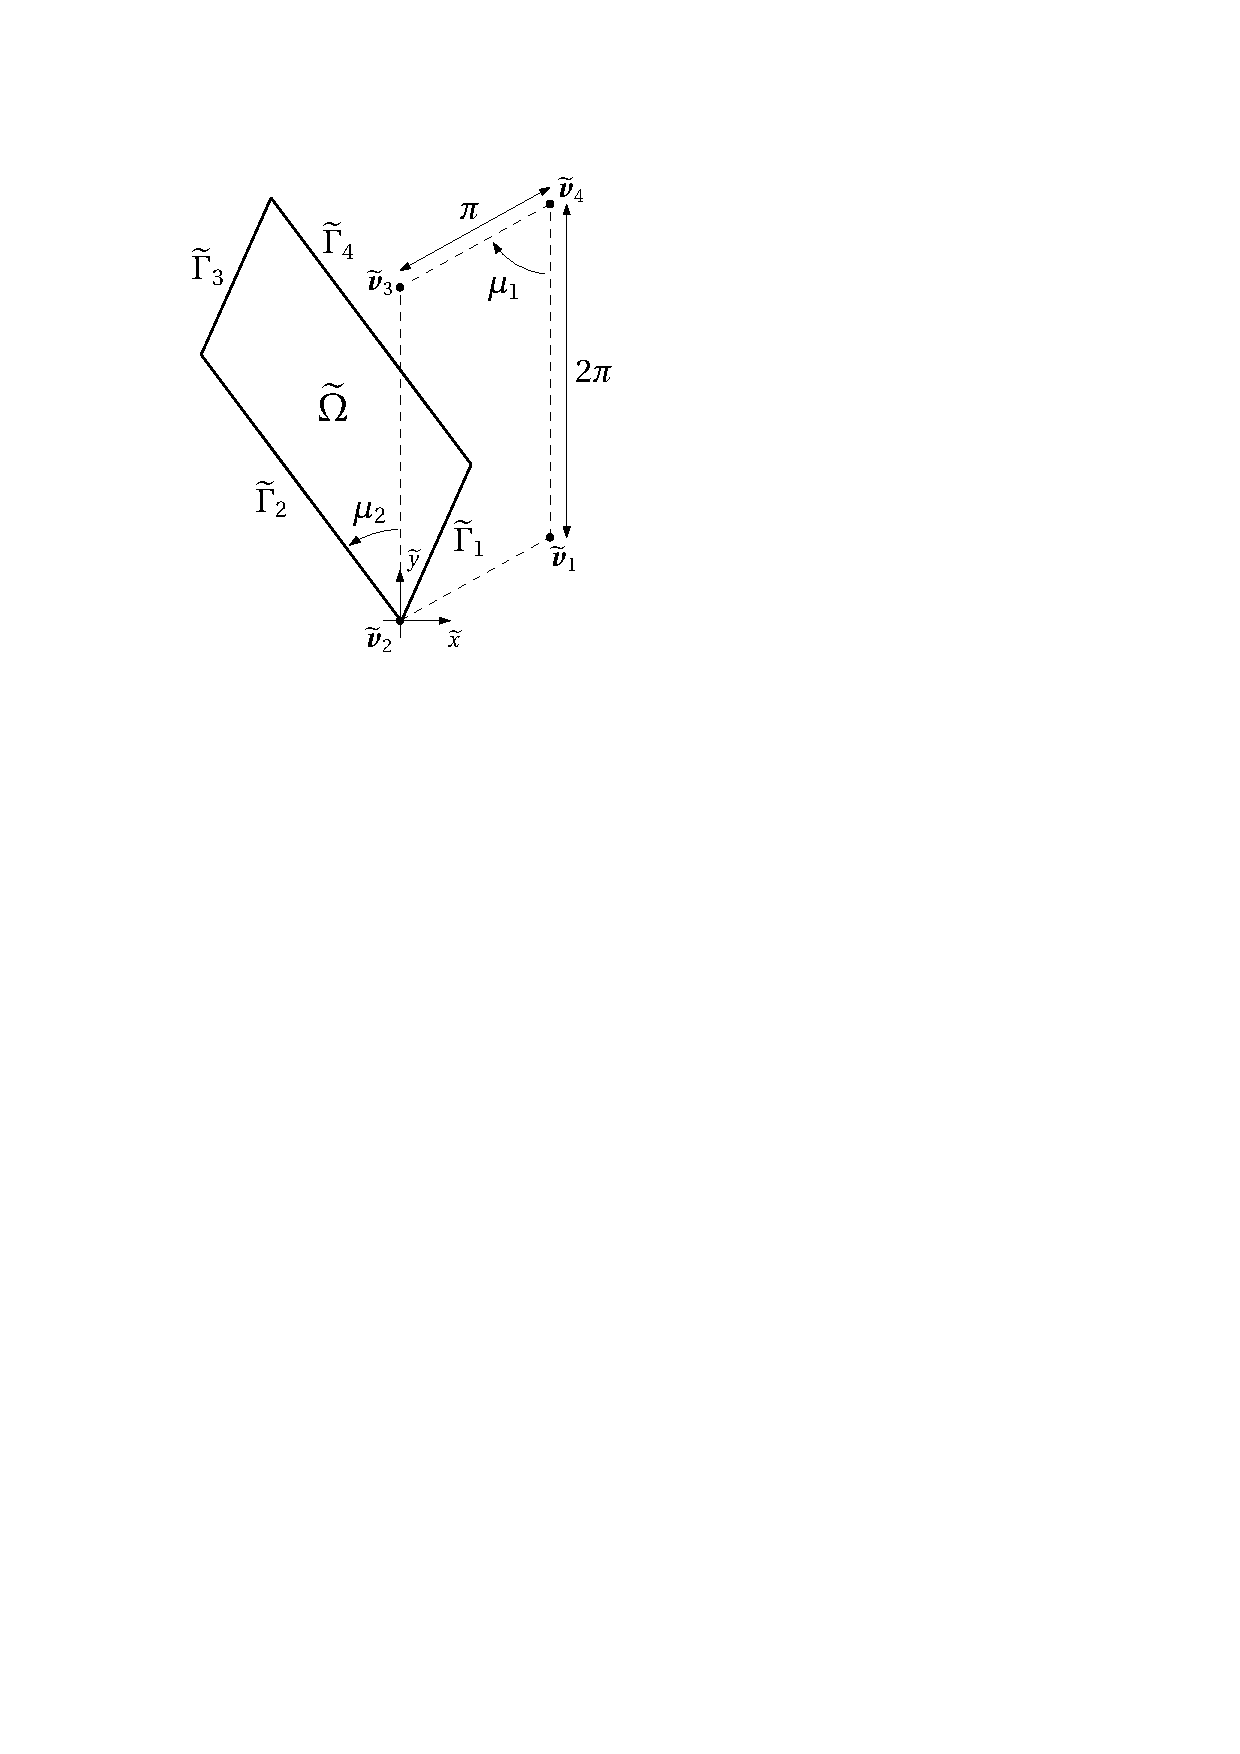
\includegraphics[scale = 0.65]{domain_square_ext}
			\end{minipage}
			\hfill
			\begin{minipage}{0.5\textwidth}
				$\mathbb{Q}(\mu_2) =
				\begin{bmatrix}
				\hspace*{-0.15cm}
				\begin{array}{cc}
					\cos(\mu_2) & -\sin(\mu_2) \\[0.1cm]
					\sin(\mu_2) & \cos(\mu_2)
				\end{array} 
				\hspace*{-0.15cm}
				\end{bmatrix}
				$ \\[0.3cm]
				$\wt{\bg{v}}_1 = \wt{\bg{v}}_1(\mu_1) = \big[ \pi \sin(\mu_1), \, \pi \cos(\mu_1) \big]^T$ \\[0.2cm]
				$\wt{\bg{v}}_2 = \wt{\bg{v}}_2(\mu_1) \equiv \big[ 0, \, 0 \big]^T$ \\[0.2cm]
				$\wt{\bg{v}}_3 = \wt{\bg{v}}_3(\mu_1) \equiv \big[ 0, \, 2 \pi \big]^T$ \\[0.2cm]
				$\wt{\bg{v}}_4 = \wt{\bg{v}}_4(\mu_1) = \big[ \pi \sin(\mu_1), \, \pi \big( 2 + \cos(\mu_1) \big) \big]^T$ \\[0.2cm]
				$\wt{\bg{\Psi}}_i(t; \, \bg{\mu}) = \mathbb{Q}(\mu_2) \left[ t \wt{\bg{v}}_i + (1-t) \wt{\bg{v}}_{i+1} \right]$ \\
				\hspace*{0.5cm} for $1 \leq i \leq 4$, with $\wt{\bg{v}}_5 \equiv \wt{\bg{v}}_1$
			\end{minipage}
			
			\vspace*{0.1cm}
			
			\caption{The quadrilateral domain used in the simulations (\emph{left}, solid line) and the parametrizations of its sides (\emph{right}).}
			\label{fig:quadrilateral-domain}
			
			\vspace*{0.45cm}
		
			\begin{minipage}{0.4\textwidth}
				\center
				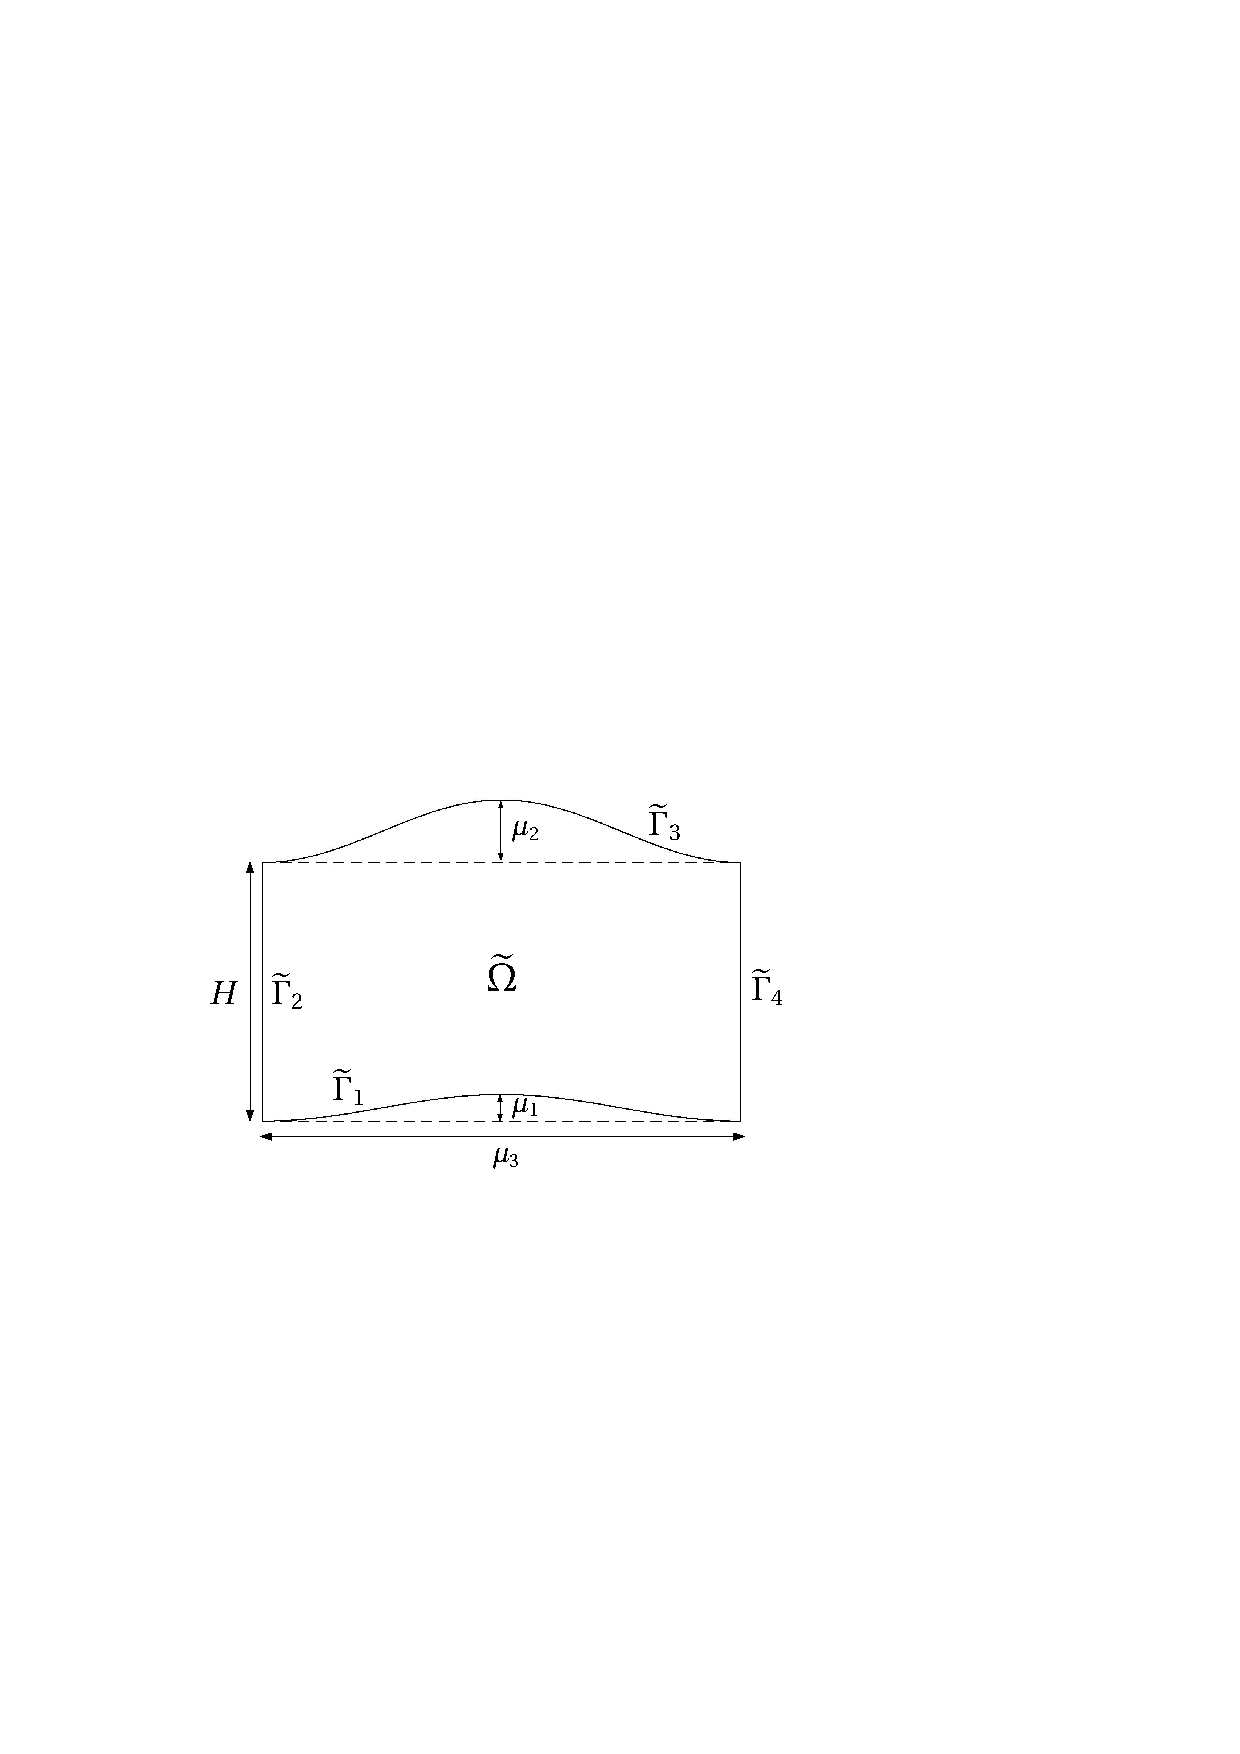
\includegraphics[scale = 0.65, trim = {0 0 0 1cm}, clip]{domain_stenosis}
			\end{minipage}
			\hfill
			\begin{minipage}{0.5\textwidth}
				$\wt{\bg{\Psi}}_1(t; \, \bg{\mu}) = \big[ \mu_3 \, (1-t), \, \mu_1 \cos\left( 2 \pi t - \dfrac{\pi}{2} \right) + \mu_1 \big]^T$ \\[0.15cm]
				$\wt{\bg{\Psi}}_2(t; \, \bg{\mu}) \equiv \big[ 0, \, H \, t \big]^T$ \\[0.15cm]
				$\wt{\bg{\Psi}}_3(t; \, \bg{\mu}) = \big[ \mu_3 \, t, \, H - \mu_2 \cos\left( 2 \pi t - \dfrac{\pi}{2} \right) - \mu_2 \big]^T$ \\[0.15cm]
				$\wt{\bg{\Psi}}_4(t; \, \bg{\mu}) = \big[ 0, \, H (1 - t) \big]^T$
			\end{minipage}
			
			\vspace*{-0.5cm}
			
			\caption{The stenosis geometry employed in the simulations (\emph{left}) and the parametrizations of its sides (\emph{right}).}
			\label{fig:stenosis-domain}
		\end{figure}
		
	\subsection{Linear test case}
	\label{section:poisson2d-1}
	
		Let $\wt{\Omega} = \wt{\Omega}(\bg{\mu})$ be the stenosis geometry shown in Fig. \ref{fig:stenosis-domain}, with $\bg{\mu} = \big( \mu_1, \, \mu_2, \, \mu_3 \big) \in \mathcal{P} = \big[-0.5, \, 0.5\big] \times \big[-0.5, \, 0.5\big] \times \big[1 , \, 5\big]$ and consider the following linear Poisson problem for $\wt{u} = \wt{u}(\bg{\mu})$:
		\begin{equation}
			\label{eq:poisson2d-1}
			\begin{cases}
				& - \wt{\Delta} \wt{u}(\bg{\mu}) = \wt{s} (\wt{x}, \, \wt{y}) = 2 \sin(\wt{x}) \cos(\wt{y}) \hspace*{0.3cm} \text{in $\wt{\Omega}(\bg{\mu})$} \, , \\
				& \wt{u}(\bg{\mu}) = \sin(\wt{\sigma}_x) \cos(\wt{\sigma}_y) \hspace*{2.175cm} \text{on $\partial \wt{\Omega}(\bg{\mu})$} \, .
			\end{cases}
		\end{equation}
		Once the problem has been re-stated over the reference domain $\Omega$ by means of the map \eqref{eq:my-bddtm} and the change of variables formulae reported in Section \ref{section:Change of variables formulae}, the discretization via finite elements yields the linear system
		\begin{equation}
			\label{eq:poisson2d-1-fe-system}
			\mathbb{A}(\bg{\mu}) \, \mathbf{u}_h(\bg{\mu}) = \mathbf{s}(\bg{\mu})
		\end{equation}
		in the nodal evaluations $\mathbf{u}_h(\bg{\mu}) \in \mathbb{R}^M$ of the high-fidelity solution $u_h(\bg{\mu})$, where the matrix $\mathbb{A}(\bg{\mu}) \in \mathbb{R}^{M \times M}$ and the vector $\mathbf{s}(\bg{\mu}) \in \mathbb{R}^M$ are defined as
		\begin{equation*}
			\begin{aligned}
				& \mathbb{A}(\bg{\mu})_{i,j} = \sum_{K \in \Omega_h} a_K(\phi_j, \, \phi_i) = \int_K \mathbb{J}_{\bg{\Phi}}^{-T}(\bg{\mu}) \nabla \phi_j \cdot \mathbb{J}_{\bg{\Phi}}^{-T}(\bg{\mu}) \nabla \phi_i ~ \big| \mathbb{J}_{\bg{\Phi}}(\bg{\mu}) \big| \, d\,K & \text{for $i$, $j = 1, \, \ldots \, , M$} \, , \\
				& \mathbf{s}(\bg{\mu})_i = \sum_{K \in \Omega_h} \int_K \big( \wt{s} \circ \bg{\Phi} \big) \, \phi_i ~ \big| \mathbb{J}_{\bg{\Phi}}(\bg{\mu}) \big| \, d\,K - \sum_{K \in \Omega_h} a_K(l_h(\bg{\mu}), \, \phi_i) & \text{for $i = 1, \, \ldots \, , M$}.
			\end{aligned}
		\end{equation*}
		Here, we recall that $K$ denotes a generic triangular element of the computational mesh $\Omega_h$, $\big\lbrace \phi_i \big\rbrace_{i = 1}^M$ is the canonical (Lagrangian) FE basis for $V_h = X_h^1 \cap H_0^1(\Omega)$, $\mathbb{J}_{\bg{\Phi}} ~ : ~ \Omega \times \mathcal{P} \rightarrow \mathbb{R}^{2 \times 2}$ represents the Jacobian (with respect to the spatial coordinates) of $\bg{\Phi}(\cdot; \bg{\mu})$, and $l_h(\bg{\mu}) \in X_h^1$ is the (discrete) lifting function. Therefore, letting $\mathbb{V} \in \mathbb{R}^{M \times L}$ represent a POD basis of rank $L$, for a given $\bg{\mu} \in \mathcal{P}$ the Galerkin projection procedure leads to the reduced system
		\begin{equation*}
			\label{eq:poisson2d-1-podg-system}
			\mathbb{A}_L(\bg{\mu}) \, \mathbf{u}_{\texttt{rb}}(\bg{\mu}) = \mathbf{s}_L(\bg{\mu})
		\end{equation*}
		in the expansion coefficients $\mathbf{u}_{\texttt{rb}}(\bg{\mu}) \in \mathbb{R}^L$, where
		\begin{equation*}
			\label{eq:poisson2d-1-podg-matrices}
			\mathbb{A}_L(\bg{\mu}) = \mathbb{V}^T \mathbb{A}(\bg{\mu}) \mathbb{V} \in \mathbb{R}^{L \times L} \hspace*{0.5cm} \text{and} \hspace*{0.5cm} \mathbf{s}_L(\bg{\mu}) = \mathbb{V}^T \mathbf{s}(\bg{\mu}) \in \mathbb{R}^L \, .
		\end{equation*}
		Hence, the assembly of the reduced-order matrices $\mathbb{A}_L(\bg{\mu})$ and $\mathbf{s}_L(\bg{\mu})$ entails their full-order counterpart $\mathbb{A}(\bg{\mu})$ and $\mathbf{s}(\bg{\mu})$. However, the (expensive) construction of these latter terms has to be entirely carried out at the online stage, due to the non-affine dependence of the map $\bg{\Phi}(\cdot; \bg{\mu})$ on $\bg{\mu}$, induced by the parametrizations $\bg{\Psi}_i(\cdot; \bg{\mu})$, $i = 1, \, 2, \, 3, \, 4$, characterizing the boundaries of the original domain $\wt{\Omega}(\bg{\mu})$ (see Fig. \ref{fig:stenosis-domain}). This clearly frustrates the advantage offered by the POD-Galerkin scheme of resorting to the resolution of a reduced system. In this respect, let us consider Fig. \ref{fig:poisson2d-1-fig1}, reporting the online run times for the FE, POD-G and POD-NN methods applied to \eqref{eq:poisson2d-1} for $N_{te} = 100$ randomly picked values of $\bg{\mu}$. The times refer to a MATLAB\textsuperscript{\textregistered} implementation of the three methods in exam, and have been measured on a laptop equipped with an Intel Core i7-6498DU @ 2.50 GHz processor. Both the RB models include $L = 15$ basis functions, constructed via proper orthogonal decomposition of $N = 100$ snapshots, computed over a triangular grid with $M = 16961$ internal vertices. Although the Galerkin projection leads to a reduction in the system size by a factor of $10^3$, no computational saving is attained for any test sample. Conversely, the POD-NN method enables an average online speed up of about $400$. This comes at the cost of an extended offline phase. Indeed, the automatic routine \ref{alg:podnn-training}, performed to find an optimal combination of the number of training samples and hidden neurons to use, takes around $2$ hours, as opposed to the few minutes required to build $N = 100$ FE snapshots (through the resolution of the system \eqref{eq:poisson2d-1-fe-system}) and compute their singular value decomposition. However, coupling POD with a neural network with $H_1 = H_2 = 35$ computing units per hidden layer and whose weights are adjusted relying upon $N_{tr} = 200$ training patterns $\big\lbrace \bg{\mu}^{(i)}, \, \mathbb{V}^T \mathbf{u}_h \big( \bg{\mu}^{(i)} \big) \big\rbrace_{i = 1}^{N_{tr}}$, with $\mathbb{V} \in \mathbb{R}^{M \times 15}$, yields (actually slightly) more accurate results than the POD-G method does, as can be inferred from Fig. \ref{fig:poisson2d-1-fig2} (\emph{right}). In particular, the POD-NN error $\bar{\varepsilon}_{\texttt{PODNN}}^{}(L)$ matches the projection error $\bar{\varepsilon}_{\mathbb{V}}^{}(L)$ for any $L \leq 15$; a convergence analysis for $L = 15$ is given in the left panel.
		
		\begin{figure}[H]
			\center
			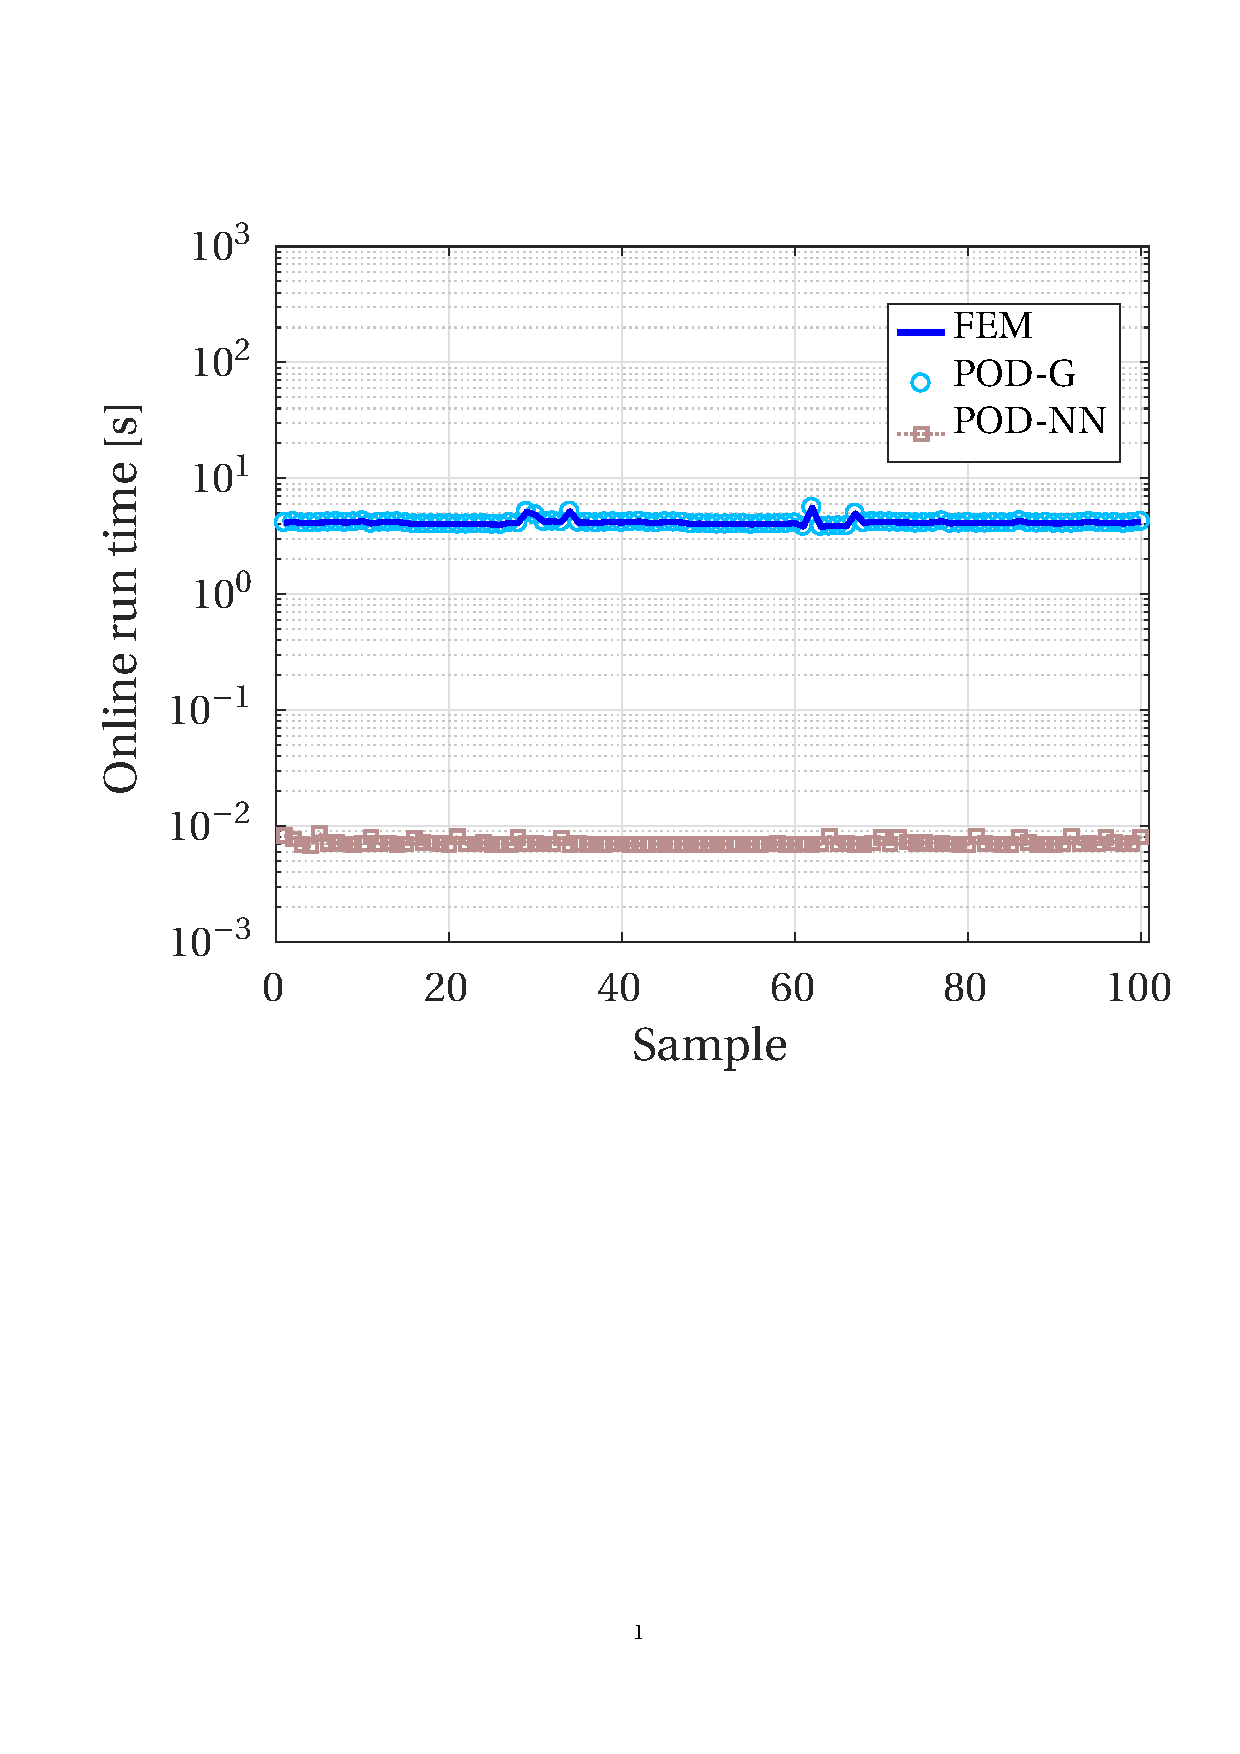
\includegraphics[scale = 0.39, trim = {1.5cm 9cm 1.25cm 3.5cm}, clip]{poisson2d_1_time}
			
			\caption{Online run times for the FE, POD-G and POD-NN methods applied to problem \eqref{eq:poisson2d-1}, for $N_{te} = 100$ randomly generated parameter values. }
			\label{fig:poisson2d-1-fig1}
		\end{figure}
		
		\vspace*{-0.2cm}
		
		\begin{figure}[H]
			\center
			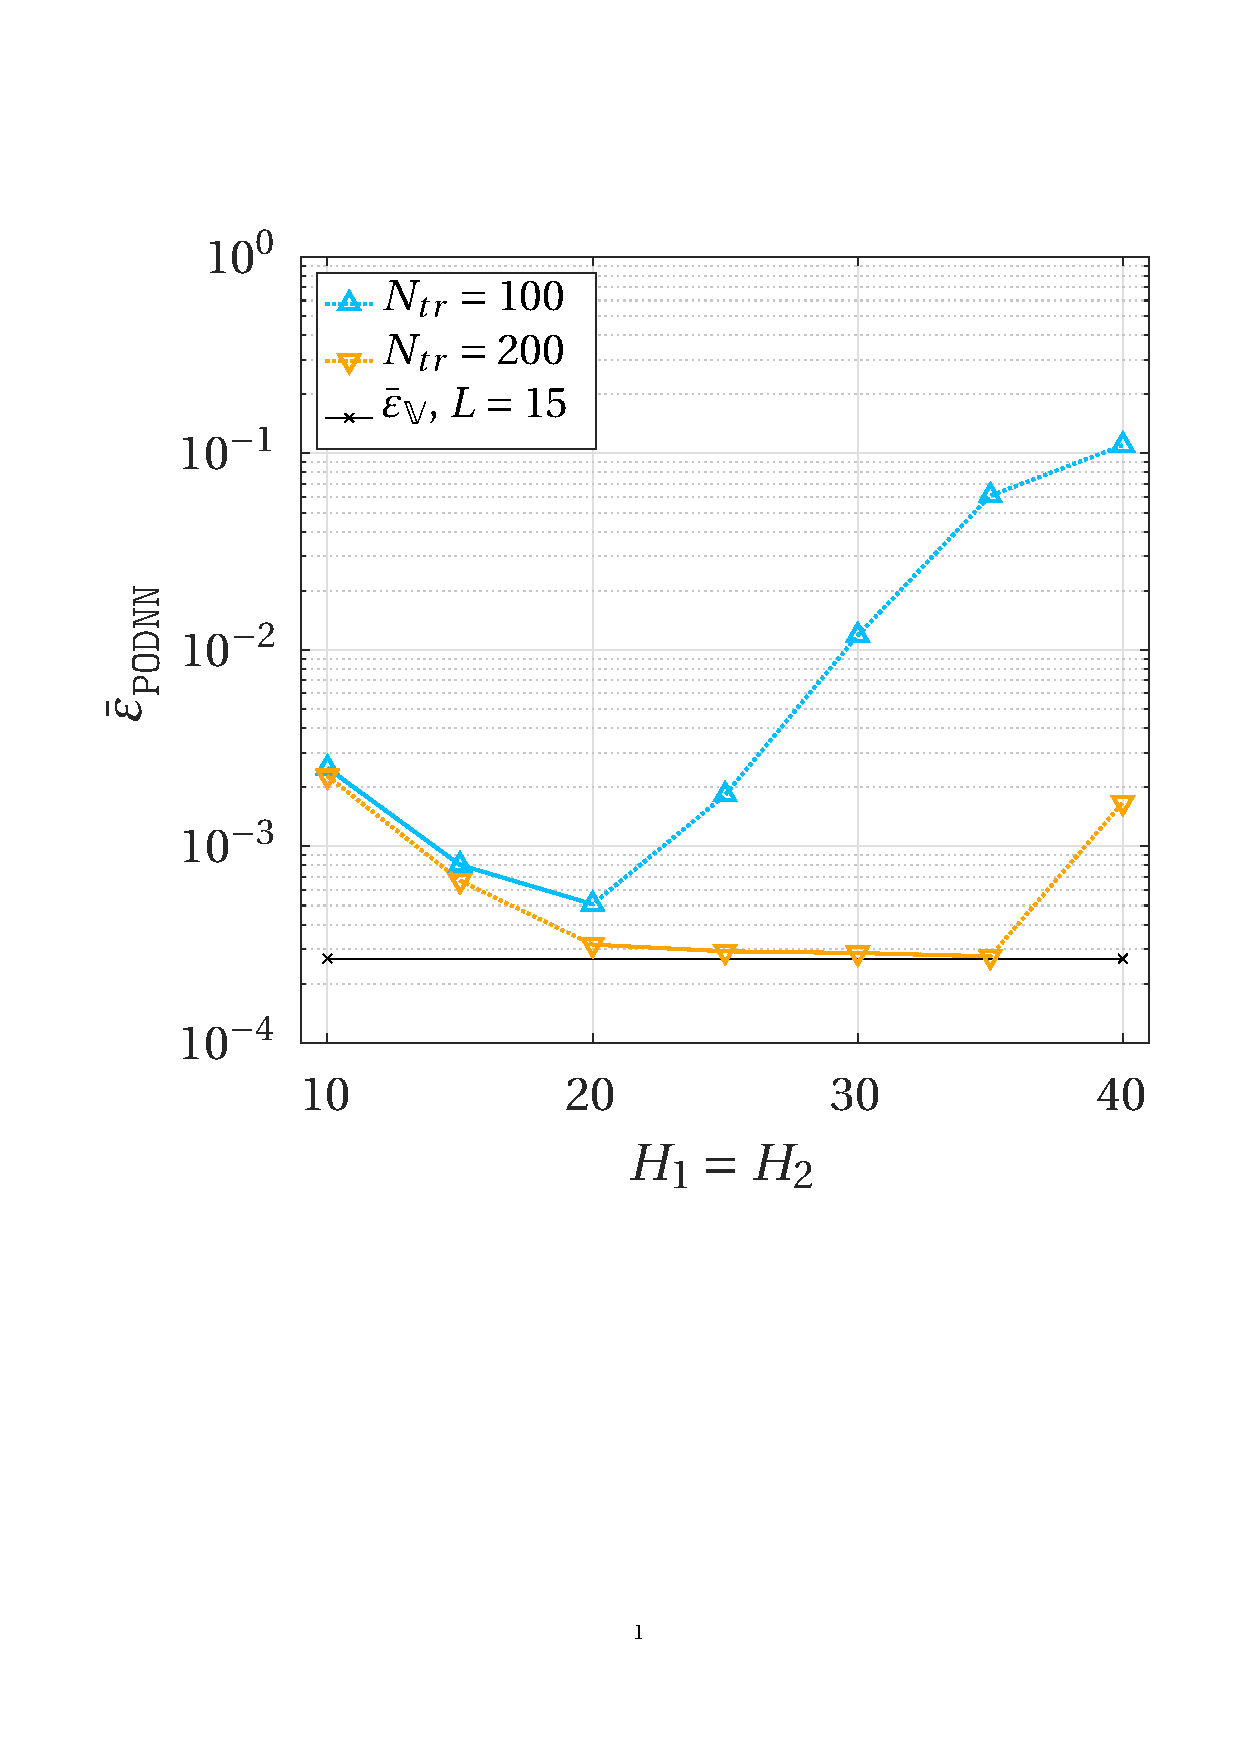
\includegraphics[scale = 0.39, trim = {1.5cm 9cm 1.5cm 3.5cm}, clip]{poisson2d_1_nn_convergence}
			\hspace*{0.5cm}
			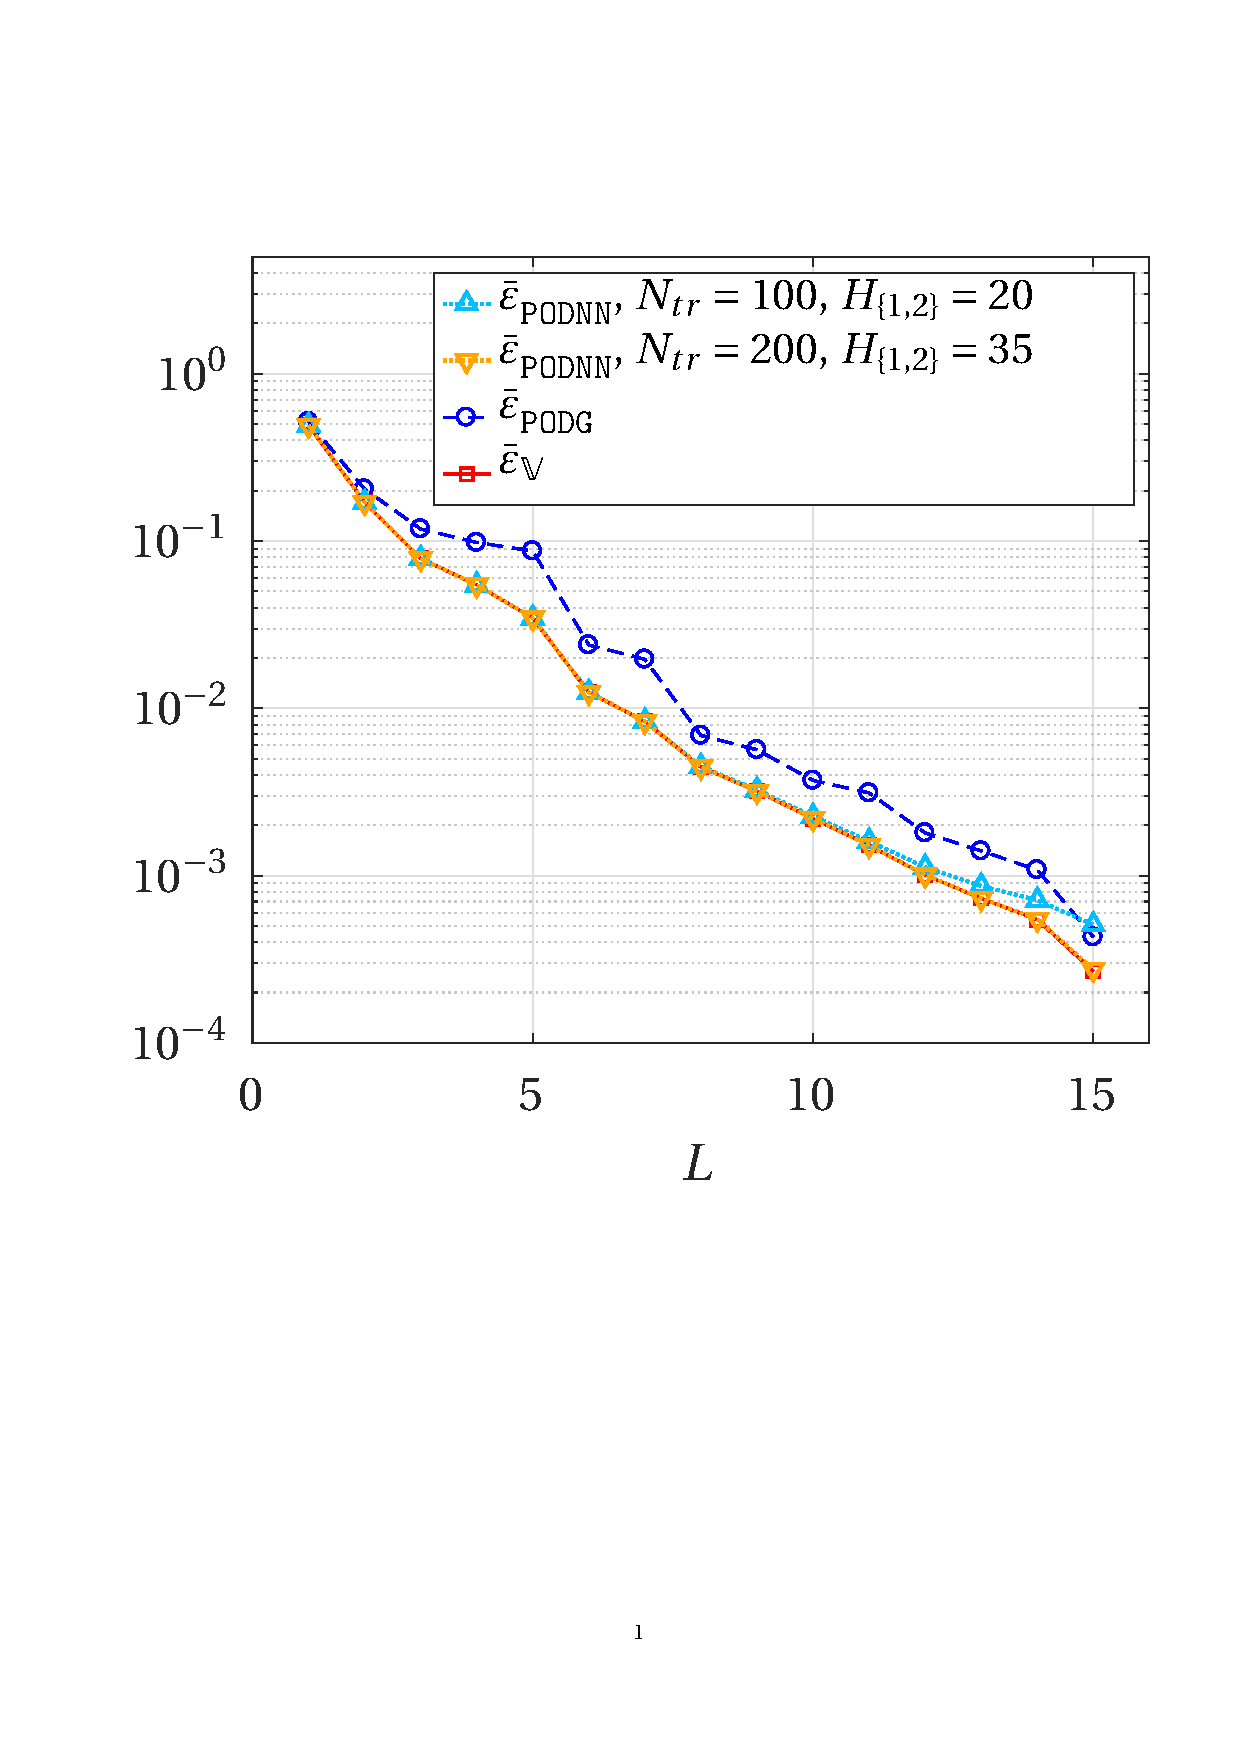
\includegraphics[scale = 0.39, trim = {1.5cm 9cm 1.5cm 3.5cm}, clip]{poisson2d_1_error_vs_rank}
			
			\caption{On the right, error analysis for the POD-G (blue dashed line) and the POD-NN (dotted lines) methods applied to problem \eqref{eq:poisson2d-1}. For the latter, a convergence analysis with respect to the number of training samples and hidden neurons used is provided on the left. The solid tracts denote the steps actually pursued by the automatic training routine \ref{alg:podnn-training}. All the results refer to neural networks exposed to $L = 15$ generalized coordinates per learning sample.}
			\label{fig:poisson2d-1-fig2}
		\end{figure}
		
	\subsection{Nonlinear test case, two parameters}
	\label{section:poisson2d-2}
	
		Let us address the upcoming BVP for a semilinear Poisson equation, stated over the parametrized quadrilateral domain $\wt{\Omega}(\bg{\mu})$ depictured in Fig. \ref{fig:quadrilateral-domain}: 
		\begin{equation}
			\label{eq:poisson2d-2}
			\begin{cases}
				& - \wt{\nabla} \cdot \big( (1 + \wt{u}(\bg{\mu})^2) ~ \wt{\nabla} \wt{u}(\bg{\mu}) \big) = \wt{s}(\wt{x}, \, \wt{y}) \hspace*{0.4cm} \text{in $\wt{\Omega}(\bg{\mu})$} \, , \\
				& \wt{u}(\bg{\mu}) = \wt{\sigma}_y \sin(\wt{\sigma}_x) \cos(\wt{\sigma}_y) \hspace*{1.65cm} \text{on $\partial \wt{\Omega}(\bg{\mu})$} \, .
			\end{cases}
		\end{equation}
		Here, the source term $\wt{s} = \wt{s}(\wt{x}, \, \wt{y})$ has been chosen so that for any $\bg{\mu} \in \mathcal{P} = \big[ \nicefrac{\pi}{4}, \, \nicefrac{3 \pi}{4} \big] \times \big[ 0, \, \nicefrac{\pi}{2} \big]$ the exact solution to the problem is given by $\wt{u}_{ex}(\wt{x}, \, \wt{y}) = \wt{y} \sin(\wt{x}) \cos(\wt{y})$. We have already referred to this problem in Section \ref{section:A POD-based RB method using neural networks}, as it lays bare the major weak point of the standard POD-Galerkin framework. In fact, as illustrated by Fig. \ref{fig:nonlinear-poisson-example}, although accurate, the POD-G method only seldomly leads to a computational saving at the online stage with respect to the FE scheme, due to the nonaffine parametric dependence of the underlying BVP. Instead, the proposed POD-NN RB procedure enables a substantial speed-up while guaranteeing high predictive precision. At this regard, Fig. \ref{fig:poisson2d-2-fig1} compares the truth (\emph{left}), POD-G (\emph{center}) and POD-NN (\emph{right}) solutions to problem \eqref{eq:poisson2d-2} for $\bg{\mu} = (0.835, \, 0.034)$. The FE discretization has been built over a mesh consisting of $M = 1921$ nodes, whereas the RB solutions have been constructed combining $L = 35$ POD basis functions, given by singular value decomposition of $N = 100$ snapshots. In particular, the POD-NN approximation has been obtained through a three-layers perceptron endowed with $H_1 + H_2 = 70$ hidden neurons and trained with $N_{tr} = 300$ learning patterns. Both RB frameworks turn out to be powerful predictive tools, as whitnessed by the good agreement between the corresponding solutions and the full-order one. This is confirmed also by the left panel in Fig. \ref{fig:poisson2d-2-fig2}, which reports the POD-G error \eqref{eq:podg-error} and the POD-NN error \eqref{eq:podnn-error} for $N_{te} = 50$ randomly picked samples not involved either in the generation of the reduced basis, nor in the networks training. However, resorting to neural networks not only yields precise responses, but also drastically reduces the time required to tackle any online query. Indeed, the right panel in Fig. \ref{fig:poisson2d-2-fig2}, offering the online run times on $\Xi_{te}$ for the two RB methodologies in exam, reveals how the POD-NN method is about $10^3$ times faster than POD-G. Yet, the search for the optimal network configuration through the routine outlined in Algorithm \ref{alg:podnn-training} unavoidably extends the offline stage of the POD-NN method. Here, it lasts around $2.5$ hours, of which only $18$ minutes are devoted to the generation of the reduced basis. Hence, considering that the FE scheme applied to \eqref{eq:poisson2d-2} takes (on average) $10$ seconds per query, the POD-NN procedure should be prefered to a direct approach only when the problem has to be solved for more than $900$ different input vector parameters.
				
		Lastly, consider Fig. \ref{fig:poisson2d-2-fig3}, which provides a convergence analysis for the POD-NN RB scheme with respect to the number $N_{tr}$ of samples used to train the network (\emph{left}) and the number $H_1 = H_2$ of internal neurons the network is endowed with (\emph{right}). For the latter plot, the results have been obtained by means of $N_{tr} = 300$ training patterns - not to incur in overfitting. Let us remark that, as for the POD-Galerkin procedure, for any fixed $N_{tr}$ and $H_i$, $i = 1$, $2$, the error yielded by the proposed method is monotonically decreasing in the number $L$ of retained basis functions, approaching or even attaining the projection error for each tested value of $L$, provided an oculate choice for $N_{tr}$ and $H_i$, $i = 1$, $2$. 
		
		\newpage
				
		\vspace*{-1.1cm}
		
		\begin{figure}[H]
			\center
			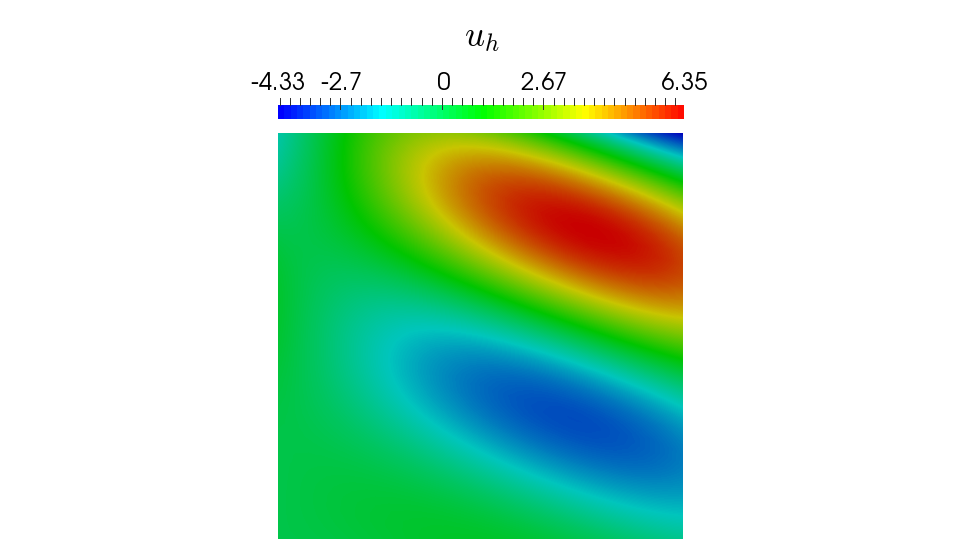
\includegraphics[scale = 0.29, trim = {8.5cm 0 8.5cm 0}, clip]{poisson2d_2_fe_solution}
			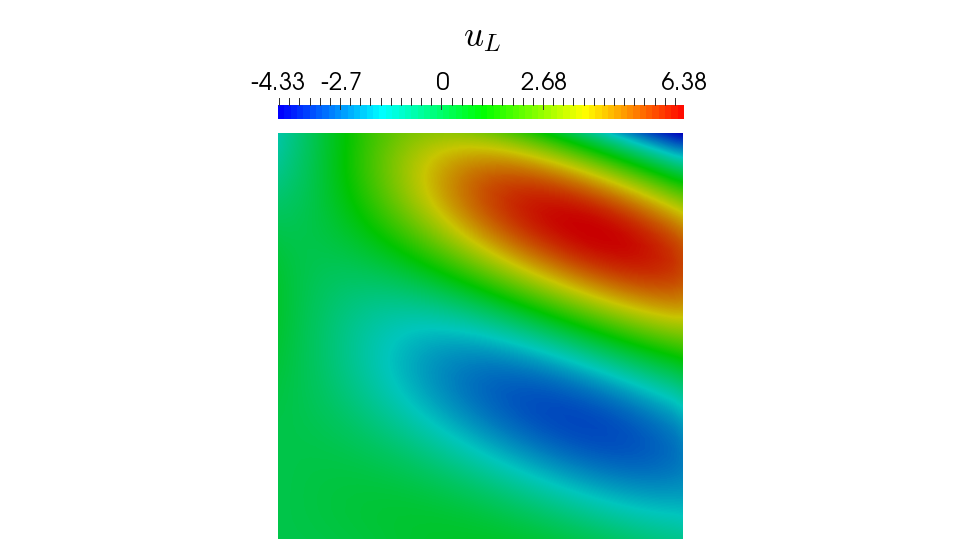
\includegraphics[scale = 0.29, trim = {8.5cm 0 8.5cm 0}, clip]{poisson2d_2_podg_solution}
			\includegraphics[scale = 0.29, trim = {8.5cm 0 8.5cm 0}, clip]{poisson2d_2_podnn_solution}
		
			\caption{Finite element (\emph{left}), POD-G (\emph{center}) and POD-NN (\emph{right}) solution to the semilinear Poisson problem \eqref{eq:poisson2d-2} re-stated over the reference domain, with $\bg{\mu} = (0.835, \, 0.034)$.}
			\label{fig:poisson2d-2-fig1}
				
		%\vspace*{-0.15cm}
		
			\center
			\includegraphics[scale = 0.4, trim = {1.5cm 9cm 1.5cm 3.5cm}, clip]{poisson2d_2_pointwise_error}
			\hfill
			\includegraphics[scale = 0.38, trim = {1.5cm 8.25cm 1.5cm 3.5cm}, clip]{poisson2d_2_time}
			
			\vspace*{-0.2cm}
			
			\caption{Online relative errors (\emph{left}) and run times (\emph{right}) for the POD-G and the POD-NN methods applied to problem \eqref{eq:poisson2d-2} for $N_{te} = 50$ randomly picked parameter values.}
			\label{fig:poisson2d-2-fig2}
		
		%\vspace*{-0.15cm}
		
			\center
			\includegraphics[scale = 0.4, trim = {1.5cm 9cm 1.5cm 3.5cm}, clip]{poisson2d_2_error_vs_rank}
			\hfill
			\includegraphics[scale = 0.4, trim = {1.5cm 9cm 1.5cm 3.5cm}, clip]{poisson2d_2_nn_convergence}
			
			\vspace*{-0.2cm}
			
			\caption{Convergence analysis for the POD-NN RB method applied to the BVP \eqref{eq:poisson2d-2}. The results have been obtained via three-layers perceptrons with $H_1 = H_2 \in \big\lbrace 15, \, 20, \, 25, \, 30, \, 35 \big\rbrace$ neurons per hidden layer, and trained with $N_{tr} \in \big\lbrace 100, \, 200, \, 300 \big\rbrace$ learning patterns. Each pattern consists of an input vector $\bg{\mu} \in \mathcal{P}$ and $L = 35$ POD coefficients $\big( \mathbf{u}_h(\bg{\mu}), \bg{\psi}_i \big)_{\mathbb{R}^M}$, $i = 1, \, \ldots \, , L$, as teaching inputs.}
			\label{fig:poisson2d-2-fig3}
		\end{figure}
				
	\subsection{Nonlinear test case, three parameters}
	\label{section:poisson2d-3}
	
		For the last test case concerning the nonlinear Poisson equation, we consider again the stenosis geometry of Fig. \ref{fig:stenosis-domain}, with $\mu_1, \, \mu_2 \in [-0.5, \, 0.5]$ and $\mu_3 \in [1, \, 5]$. The differential problem we deal with in this section reads:
		\begin{equation}
			\label{eq:poisson2d-3}
			\begin{cases}
				& - \wt{\nabla} \cdot \big( \exp(\wt{u}(\bg{\mu})) ~ \wt{\nabla} \wt{u}(\bg{\mu}) \big) = \wt{s}(\wt{x}, \, \wt{y}) \hspace*{0.45cm} \text{in $\wt{\Omega}(\bg{\mu})$} \, , \\
				& \wt{u}(\bg{\mu}) = \wt{\sigma}_x \sin(\pi \, \wt{\sigma}_x) \cos(\pi \, \wt{\sigma}_y) \hspace*{1.0cm} \text{on $\partial \wt{\Omega}(\bg{\mu})$} \, .
			\end{cases}
		\end{equation}
		with the source term $\wt{s} = \wt{s}(\wt{x}, \, \wt{y})$ properly chosen so that the exact solution to the problem is given by $\wt{u}_{ex}(\wt{x}, \, \wt{y}) = \wt{y} \sin(\pi \, \wt{x}) \cos(\pi \, \wt{y})$ for all $\bg{\mu} \in \mathcal{P}$. Albeit the state equation shows up an exponential nonlinearity and the computational domain presents curvilinear boundaries, both the RB methodologies studied in this work provide accurate solutions, close to the optimal one, i.e., the projection of the truth solution $u_h(\bg{\mu})$ onto the reduced space $V_{\texttt{rb}}$. This can be drawn from Fig. \ref{fig:poisson2d-3-fig1}, offering the finite element solution (\emph{top left}) to \eqref{eq:poisson2d-3} when $\bg{\mu} = (0.349, \, -0.413, \, 4.257)$, and the pointwise errors committed by either the projection onto $V_{\texttt{rb}}$ (\emph{top right}), or the POD-G method (\emph{bottom left}), or the POD-NN method (\emph{bottom right}). The computational mesh employed consists of $2792$ nodes, resulting in $M = 2632$ degrees of freedom (as many as the inner nodes) for the FE scheme. The reduced space $V_{\texttt{rb}}$ is generated by $L = 30$ basis functions, given by POD of an ensemble of $N = 100$ snapshots. Specifically, the results concerning the POD-NN method have been obtained by employing a neural network equipped with $H_1 = H_2 = 35$ neurons per hidden layer and trained relying upon $N_{tr} = 200$ learning samples. In this way, the POD-NN procedure leads to an error field which shows similar patterns to those featured by the projection error field. This is not surprising, due to the way neural networks are trained within the POD-NN framework (see Section \ref{section:A POD-based RB method using neural networks}). 
				
		\vspace*{-0.2cm}
						
		\begin{figure}[H]
			\center
			\subfloat{\includegraphics[scale = 0.275, trim = {1cm 3cm 4cm 2.5cm}, clip]{poisson2d_3_fe_solution}}
			\subfloat{\includegraphics[scale = 0.275, trim = {1cm 3cm 4cm 2.5cm}, clip]{poisson2d_3_error_projection}} \\[-0.2cm]
			\subfloat{\includegraphics[scale = 0.275, trim = {1cm 3cm 4cm 2.5cm}, clip]{poisson2d_3_error_podg}}
			\subfloat{\includegraphics[scale = 0.275, trim = {1cm 3cm 4cm 2.5cm}, clip]{poisson2d_3_error_podnn}}
			
			%\vspace*{-0.2cm}
			
			\caption{FE solution (\emph{top left}) to the Poisson problem \eqref{eq:poisson2d-3} with $\bg{\mu} = (0.349, \, -0.413, \, 4.257)$, and pointwise errors yielded by either its projection onto $V_{\texttt{rb}}$ (\emph{top right}), or the POD-G method (\emph{bottom left}), or the POD-NN method (\emph{bottom right}). The results have been obtained by considering $L = 30$ POD modes.}
			\label{fig:poisson2d-3-fig1}
		\end{figure}	
		
		\begin{figure}[H]
			\center
			\includegraphics[scale = 0.43, trim = {1.5cm 9.6cm 1.5cm 3.8cm}, clip]{poisson2d_3_error_vs_rank}
			\hfill
			\includegraphics[scale = 0.41, trim = {1.5cm 8.9cm 1.5cm 3.8cm}, clip]{poisson2d_3_time}
			
			\caption{Error analysis (\emph{left}) and online CPU time (\emph{right}) for the POD-G and the POD-NN methods applied to problem \eqref{eq:poisson2d-3} for $N_{te} = 50$ randomly picked parameter values. The reduced basis have been generated via POD, relying on $N = 100$ snapshots. The second plot refers to RB models including $L = 30$ modal functions; within the POD-NN framework, a neural network emboding $35$ neurons per inner layer has been used.}
			\label{fig:poisson2d-3-fig2}
		\end{figure}
		
		\vspace*{-0.2cm}
		
		A quantitative evidence of the efficacy of the RB approximations is given by the plot on the left in Fig. \ref{fig:poisson2d-3-fig2}, reporting a convergence analysis for both the POD-G and the POD-NN methods with respect to the number $L$ of retained modal basis functions. As usual, the error has to be intended as an average over a parameter data set $\Xi_{te}$, here consisting of $N_{te} = 50$ samples. However, the second plot of Fig. \ref{fig:poisson2d-3-fig2} reveals how the former scheme produces a response for any online query approximately $10^4$ times slowlier than the proposed POD-NN procedure does, preventing any computational gain with respect to the finite element scheme. This assertion can also be extended to the memory demand. In fact, in addition to the assembly of the full-order residual vector $\mathbf{G}_h(\cdot;\bg{\mu}) \in \mathbb{R}^M$ and the associated Jacobian $\mathbb{J}_h(\cdot;\bg{\mu}) \in \mathbb{R}^{M \times M}$, the online phase of the POD-G RB method requires the storage of the POD basis $\mathbb{V} \in \mathbb{R}^{M \times L}$. Here, $M = 2632$ and $L = 30$, with the (sparse) Jacobian featuring $18388$ non-zero entries. Hence, recalling that a float occupies $4$ bytes in memory, the memory footprint approximately amounts to $400$ Kb. Instead, the POD-NN method requires only the underpinning neural network to tackle any query. Therefore, assuming $35$ computing units within both inner layers, we need a bit more than $9$ Kb of RAM, coincident with the space necessary to save the synaptical and bias weights characterizing the network.
		
		Let us now dive deeplier into the analysis of the first plot of Fig. \ref{fig:poisson2d-3-fig2}. Within the POD-NN framework, when the proper orthogonal decomposition of a set of $N = 100$ snapshots is coupled with a three-layers perceptron with $35$ neurons per hidden layer, trained to approximate the map \eqref{eq:map-to-approximate} relying on $N_{tr} = 200$ learning patterns, for each $L \leq 30$ the yielded relative error is smaller than the error committed by the POD-Galerkin procedure. Yet, halfing the number of learning patterns employed, the POD-NN error curve stops decreasing at $L = 20$, then incurring in a plateu. In this regard, Fig. \ref{fig:poisson2d-3-fig3} suggests that as the size of the available training set decreases, one should coherently reduce the amount of computing units to be embodied in the network, thus to limit the risk of overfitting. This is in agreement with the results previously discussed in this chapter (see, e.g., Fig. \ref{fig:poisson1d-2-fig2} and Fig. \ref{fig:poisson2d-1-fig2}).
						
		\begin{figure}[H]
			\center
			\vspace*{-0.4cm}
			\includegraphics[scale = 0.42, trim = {1.5cm 9.6cm 1.5cm 3.5cm}, clip]{poisson2d_3_nn_convergence}
			\hfill
			\includegraphics[scale = 0.425, trim = {1.5cm 9.8cm 1.5cm 3.5cm}, clip]{poisson2d_3_nn_comparison}
						
			\caption{Convergence analysis with respect to the number of hidden neurons (\emph{left}) and modal functions (\emph{right}) used within the POD-NN framework applied to problem \eqref{eq:poisson2d-3}. The results provided in the first plot have been obtained using $L = 30$ modes; the solid tracts refer to the steps performed by Algorithm \ref{alg:podnn-training}.}
			\label{fig:poisson2d-3-fig3}
		\end{figure}	
		
		The distinguishing and novel feature of the POD-NN method is represented by the employment of multi-layer perceptrons to recover the coefficients of the reduced model. To motivate this choice, let us pursue a more traditional approach to tackle the interpolation step by resorting to cubic splines \cite{Deb78}. To this end, let $\Xi_{\delta} \subset \mathcal{P}$ be a tensor-product grid on the parameter domain, based on Chebyshev nodes \footnote{For a given natural number $n$, the Chebyshev nodes in the interval $(a, \, b)$ are \[ x_k = \dfrac{1}{2}(a + b) + \dfrac{1}{2}(b - a) \, \cos \left( \dfrac{2k - 1}{2n} \pi \right) \, , \] for $k = 1, \, \ldots \, , n$}. In the offline phase, for each $\bg{\mu}_{\delta} \in \Xi_{\delta}$ we compute the truth solution $\mathbf{u}_h(\bg{\mu}_{\delta}) \in \mathbb{R}^M$ and we extract the expansion coefficients $\mathbb{V}^T \mathbf{u}_h(\bg{\mu}_{\delta}) \in \mathbb{R}^L$. At the online stage, given a new parameter value $\bg{\mu} \in \mathcal{P}$, the $i$-th expansion coefficient, $i = 1, \, \ldots \, , L$, is sought by cubic spline interpolation of the samples \[ \big\lbrace \big( \bg{\mu}_{\delta}, \, \big( \mathbb{V}^T \mathbf{u}_h(\bg{\mu}_{\delta}) \big)_i \big) \big\rbrace_{\bg{\mu}_{\delta} \in \Xi_{\delta}} \, . \] Hence, denoting by $\mathbf{u}_{\texttt{rb}}^{\texttt{CS}}(\bg{\mu}) \in \mathbb{R}^L$ the so-constructed approximation of $\mathbb{V}^T \mathbf{u}_h(\bg{\mu})$, the reduced-order approximation of $\mathbf{u}_h(\bg{\mu})$ is given by $\mathbf{u}_L^{\texttt{CS}}(\bg{\mu}) = \mathbb{V} \, \mathbf{u}_{\texttt{rb}}^{\texttt{CS}}(\bg{\mu})$. Similarly to the POD-G and the POD-NN method, the accuracy of the resulting POD-CS procedure can be assessed by evaluating the relative error $\varepsilon_{\texttt{PODCS}}^{}(L, \, \bg{\mu})$, defined as
		\begin{equation*}
			\label{eq:podcs-error}
			\varepsilon_{\texttt{PODCS}}^{}(L, \, \bg{\mu}) = \dfrac{\norm{\mathbf{u}_h(\bg{\mu}) - \mathbf{u}_L^{\texttt{CS}}(\bg{\mu})}}{\norm{\mathbf{u}_h(\bg{\mu})}} = \dfrac{\norm{\mathbf{u}_h(\bg{\mu}) - \mathbb{V} \, \mathbf{u}_{\texttt{rb}}^{\texttt{CS}}(\bg{\mu})}}{\norm{\mathbf{u}_h(\bg{\mu})}} \, ,
		\end{equation*}
		on a test parameter set $\Xi_{te} \subset \mathcal{P}$, with $\Xi_{te} \cap \Xi_{\delta} = \emptyset$.
		
		For the Poisson problem \eqref{eq:poisson2d-3}, we report in the left plot of Fig. \ref{fig:poisson2d-3-fig4} the relative errors, averaged on $\Xi_{te}$, yielded by both the POD-CS and the POD-NN methods. For the former, we provide the results obtained on tensor-product grids consisting of $N_{\delta}$ interpolation points, with $N_{\delta} \in \lbrace 5^3, \, 7^3, \, 10^3 \rbrace$. For the latter, $H_1 = H_2 = 35$ neurons per hidden layer and $N_{tr} = 200$ training patterns have been used. Although the online performance of the two procedures are basically the same, as shown by the second plot in Fig. \ref{fig:poisson2d-3-fig4}, we observe that the level of predictive accuracy enabled by the POD-NN method can be attained or at least approached by cubic spline interpolation only when this relies on $N_{\delta} = 1000$ samples. In fact, as mentioned in the Introduction, a standard interpolation technique may require a large number of samples, thus snapshots, to be able to enforce the constraints characterizing the nonlinear manifolds which the reduced bases typically belong to \cite{Ams10}. Hence, although this approach provides a valuable alternative for paremetrized problems with a few parameters, it may be unfeasible in real-life applications, involving hundreads of parameters. Conversely, the secret hope behind the choice of a neural network-based function regression is that of bounding the amount of required snapshots also in case of a high-dimensional parameter domain, thus to justify the overheads due to the training phase.
		
		\begin{figure}[t!]
			\center
			\includegraphics[scale = 0.43, trim = {1.5cm 9.6cm 1.5cm 3.8cm}, clip]{poisson2d_3_cs_error}
			\hfill
			\includegraphics[scale = 0.41, trim = {1.5cm 8.9cm 1.5cm 3.8cm}, clip]{poisson2d_3_cs_time}
			
			\caption{Average relative errors (\emph{left}) and online run times (\emph{right}) on $\Xi_{te}$ for the POD-CS and the POD-NN methods applied to problem \eqref{eq:poisson2d-3}. For the latter, the results refer to an MLP equipped with $H_1 = H_2 = 35$ neurons per hidden layer.}
			\label{fig:poisson2d-3-fig4}
		\end{figure}
		
	\vspace*{0.3cm}
		
	\section{The lid-driven cavity problem}
	\label{section:The lid-driven cavity problem}
	
		In this section, we tackle the reduced-basis modeling of the steady uncompressible Navier-Stokes equations \eqref{eq:ns-differential} via the POD-G and the POD-NN procedure. Specifically, we address the numerical simulation of a viscous flow within a parallelogram-shaped cavity, illustrated in Fig. \ref{fig:dc-domain} (\emph{left}). The geometry of the domain is affected by three parameters: $\mu_1 \in [1, \, 2]$ and $\mu_2 \in [1, \, 2]$ define the length of the horizontal and slanting (possibly vertical) edges, respectively, whereas $\mu_3 \in \big[ \nicefrac{\pi}{6}, \, \nicefrac{5 \pi}{6} \big]$ denotes the angle between the oblique sides and the positive $\wt{x}$-semiaxis. The Dirichlet boundary conditions enforced on the velocity field, graphically represented in Fig. \ref{fig:dc-domain} (\emph{right}), are such that the flow is driven by a unit horizontal velocity at the top boundary \cite{Per02}. For this reason, this benchmark is typically referred to as the \emph{lid-driven cavity} problem. In addition, to retain the uniqueness of the solution, we fix the pressure at the lower-left corner \cite{Dho14}. Therefore, to properly resolve the steep velocity gradient near the upper boundary and the pressure singularities at the top corners, the computational mesh $\Omega_h$ (Fig. \ref{fig:dc-mesh}) is refined in the upper part of the domain, leading to $M_{\bg{v}} = 4868$ degrees of freedom for $\bg{v}$ and $M_p = 691$ nodal values for $p$. 
		
		Figure \ref{fig:dc-solutions-different-domains} shows the velocity streamlines (\emph{top}) and the pressure distribution (\emph{bottom}) obtained through the FE method for, from the left to the right, $\bg{\mu} = \big( 1, \, \nicefrac{2}{\sqrt{3}}, \, \nicefrac{2 \pi}{3} \big)$, $\bg{\mu} = \big( 1, \, 1, \, \nicefrac{\pi}{2} \big)$ or $\bg{\mu} = \big( 1, \, \nicefrac{2}{\sqrt{3}}, \, \nicefrac{\pi}{6} \big)$. The results refer to a Reynold's number of $400$. The Reynold's number is an adimensional group, defined as the ratio between the inertia and viscous (or friction) force. For the specific problem at hand, it reads:
		\begin{equation*}
			\vspace*{-0.1cm}
			Re = \dfrac{\max \big\lbrace \mu_1, \, \mu_2 \big\rbrace}{\nu(\bg{\mu})} \, ,
		\end{equation*}
		with $\nu = \nu(\bg{\mu})$ being the dynamic viscosity of the fluid. In our analyses, $\nu(\bg{\mu})$ is adapted according to the geometry so that the Reynold's number is either $200$ or $400$ \vspace*{0.2cm} \footnote{We would like to point out that these values for the Reynold's number have been chosen sufficiently low, so that the flow can be reasonably treated as steady.}.
				
		\vspace*{-0.3cm}
		
		\begin{figure}[t!]
			\center
			\includegraphics[scale = 0.65]{dc_domain}
			\hspace*{1cm}
			\includegraphics[scale = 0.65]{dc_domain_bc}
			
			\caption{Computational domain (\emph{left}) and enforced velocity at the boundaries (\emph{right}) for the lid-driven cavity problem for the uncompressible Navier-Stokes equations.}
			\label{fig:dc-domain}
		\end{figure}
				
		%\vspace*{-0.7cm}
				
		\begin{figure}[H]
			\center
			\includegraphics[scale = 0.375, trim = {2cm 9cm 1.5cm 3.5cm}, clip]{dc_mesh}
			
			\vspace*{-0.2cm}
			
			\caption{The computational mesh $\Omega_h$ used in the simulations.}
			\label{fig:dc-mesh}
		\end{figure}
				
		As mentioned above, the moving lid induces a large velocity gradient close to the top boundary, while it only slightly affects the fluid in the lower part of the cavity. In turn, this gives rising to two vortices. For $\mu_3 \geq \nicefrac{\pi}{2}$ a large recirculation area expands throughout the domain in the top-down direction, with a smaller vortex, characterized by much lower velocities, appearing in the lower-right corner. By contrast, for $\mu_3 = \nicefrac{\pi}{6}$ the two vortices share the domain almost equally. Actually, if we further decrease the shear angle $\mu_3$, we would note the generation of a third micro-vortex next to the bottom-left corner. In this respect, consider Fig. \ref{fig:dc-solutions-different-reynolds}, providing the velocity streamlines for the lid-driven cavity benchmark with $\bg{\mu} = \big( 1, \, \sqrt{2}, \, \nicefrac{\pi}{4} \big)$ and for a Reynold's number of either $200$ (\emph{left}) or $400$ (\emph{right}). It is worth noticing that as the Reynold's number decreases, the extent of the upper recirculation area increases, coherently with the augment of the dynamic viscosity. 
		
		Conversely to the velocity distribution, the pressure field does not undergo remarkable alterations across the parameter space. For all the configurations, a low-pressure region takes place at the upper-left corner of the domain and in the center of the major vortex (although it may be not clearly visible). Instead, the upper-right corner represents a stagnation point for the $\wt{x}$-velocity, and so therein the pressure assumes larger values than in the rest of the cavity \cite{Dho14}. 
						
		\begin{figure}[H]
			\center 
			\subfloat[$\bg{\mu} = \big( 1, \, \nicefrac{2}{\sqrt{3}}, \, \nicefrac{2 \pi}{3} \big)$]{\includegraphics[scale = 0.25, trim = {6.5cm 0 5.5cm 0}, clip]{dc_400_vel_fem_solution_1}}
			\subfloat[$\bg{\mu} = \big( 1, \, 1, \, \nicefrac{\pi}{2} \big)$]{\includegraphics[scale = 0.25, trim = {7.5cm 0 7.5cm 0}, clip]{dc_400_vel_fem_solution_2}}
			\subfloat[$\bg{\mu} = \big( 1, \, \nicefrac{2}{\sqrt{3}}, \, \nicefrac{\pi}{3} \big)$]{\includegraphics[scale = 0.25, trim = {4.8cm 0 5.5cm 0}, clip]{dc_400_vel_fem_solution_3}} \\
			\subfloat[$\bg{\mu} = \big( 1, \, \nicefrac{2}{\sqrt{3}}, \, \nicefrac{2 \pi}{3} \big)$]{\includegraphics[scale = 0.25, trim = {6.5cm 0 5.5cm 0}, clip]{dc_400_p_fem_solution_1}}
			\subfloat[$\bg{\mu} = \big( 1, \, 1, \, \nicefrac{\pi}{2} \big)$]{\includegraphics[scale = 0.25, trim = {7.5cm 0 7.5cm 0}, clip]{dc_400_p_fem_solution_2}}
			\subfloat[$\bg{\mu} = \big( 1, \, \nicefrac{2}{\sqrt{3}}, \, \nicefrac{\pi}{3} \big)$]{\includegraphics[scale = 0.25, trim = {5cm 0 5.5cm 0}, clip]{dc_400_p_fem_solution_3}}
					
			\caption{Velocity streamlines (\emph{top}) and pressure plot (\emph{bottom}) for the lid-driven cavity problem, computed through the FE method. Three different parameter values are considered; for all configurations, the Reynold's number is $400$.}
			\label{fig:dc-solutions-different-domains}
		\end{figure}
		
		\clearpage
		
		\begin{figure}[t!]
			\center
			\subfloat[$\bg{\mu} = \big( 1, \, \sqrt{2}, \, \nicefrac{\pi}{4} \big)$, $Re = 200$]{\includegraphics[scale = 0.29, trim = {3cm 0 5cm 0cm}, clip]{dc_200_vel_fem_solution_4}}
			\subfloat[$\bg{\mu} = \big( 1, \, \sqrt{2}, \, \nicefrac{\pi}{4} \big)$, $Re = 400$]{\includegraphics[scale = 0.29, trim = {3cm 0 5cm 0cm}, clip]{dc_400_vel_fem_solution_5}} 
			
			\caption{Velocity streamlines for the lid-driven cavity benchmark with $\bg{\mu} = \big( 1, \, \sqrt{2}, \, \nicefrac{\pi}{4} \big)$ and either $Re = 200$ (\emph{left}) or $Re = 400$ (\emph{right}). The solutions have been computed via $\mathbb{P}^2$-$\mathbb{P}^1$ finite elements.}
			\label{fig:dc-solutions-different-reynolds}
		\end{figure}
		
		Moving to the reduced-order modeling of the parametrized problem of interest, Fig. \ref{fig:dc-modal-functions} reports the first $5$ modal functions for the velocity $\bg{v}_h = \bg{v}_h(\bg{\mu})$ (\emph{left}), the supremizer solution $\bg{s}_h = \bg{s}_h(\bg{\mu})$ (\emph{center}) and the pressure $p_h = p_h(\bg{\mu})$ (\emph{right}) for $Re = 200$. These have been respectively obtained via proper orthogonal decomposition of the collections of snapshots $\big\lbrace \mathbf{v}_h \big( \bg{\mu}^{(i)} \big) \big\rbrace_{i = 1}^N$, $\big\lbrace \mathbf{s}_h \big( \bg{\mu}^{(i)} \big) \big\rbrace_{i = 1}^N$ and $\big\lbrace \mathbf{p}_h \big( \bg{\mu}^{(i)} \big) \big\rbrace_{i = 1}^N$, with $\Xi_N = \big\lbrace \bg{\mu}^{(i)} \big\rbrace_{i = 1}^N \subset \mathcal{P}$ a training sample generated through latin hypercube sampling. Here, $N = 100$. We recall that each (discrete) supremizer $\mathbf{s}_h \big( \bg{\mu}^{(i)} \big)$, $i = 1, \, \ldots \, , N$, is related to the corresponding pressure snapshot $\mathbf{p}_h \big( \bg{\mu}^{(i)} \big)$ through the linear system \eqref{eq:supremizer-system}. Then, within the POD-Galerkin RB framework, a reduced-order approximation for the velocity field is searched in the enriched space 
		\begin{equation*}
			\overline{V}_{\texttt{rb}}^{\bg{v}} = \text{span} \big\lbrace \psi_1^{\bg{v}}, \, \ldots \, , \psi_{L_{\bg{v}}}^{\bg{v}}, \, \psi_1^{\bg{s}}, \, \ldots \, , \psi_{L_{\bg{s}}}^{\bg{s}} \big\rbrace \, ,
		\end{equation*}
		of dimension $\overline{L}_{\bg{v}} = L_{\bg{v}} + L_{\bg{s}}$, where $\big\lbrace \psi_i^{\bg{v}} \big\rbrace_{i = 1}^{L_{\bg{v}}}$ (respectively, $\big\lbrace \psi_i^{\bg{s}} \big\rbrace_{i = 1}^{L_{\bg{s}}}$) denote the FE functions associated with the first $L_{\bg{v}}$ (resp., $L_{\bg{s}}$) left singular vectors of the snapshot matrix $\mathbb{S}_{\bg{v}}$ (resp., $\mathbb{S}_{\bg{s}}$). Upon considering a sufficiently large number of supremizer basis functions, the stability at the reduced level follows from Proposition \ref{proposition:supremizer-enrichment}. In \cite{Bal14}, several numerical evidences suggest that a proper value for $L_{\bg{s}}$ should lay in between $L_p / 2$ and $L_p$, with $L_p$ the number of pressure POD modes included in the RB model. In our simulations, we set $L_{\bg{s}} = L_p = L_{\bg{v}}$, resulting in a stable reduced (nonlinear) system in $L = 3 \, L_{\bg{v}}$ unknowns.
		
		Concerning the POD-NN procedure, for any $\bg{\mu} \in \mathcal{P}$, reduced-order discretizations $\mathbf{v}_{L_{\bg{v}}}^{\texttt{NN}}(\bg{\mu})$ and $\mathbf{p}_{L_p}^{\texttt{NN}}(\bg{\mu})$ of $\bg{v}(\bg{\mu})$ and $p(\bg{\mu})$, respectively, are sought in the form
		\begin{equation*}
			\mathbf{v}_{L_{\bg{v}}}^{\texttt{NN}}(\bg{\mu}) = \mathbb{V}_{\bg{v}} \, \mathbf{v}_{\texttt{rb}}^{\texttt{NN}}(\bg{\mu}) \hspace*{0.5cm} \text{and} \hspace*{0.5cm} \mathbf{p}_{L_p}^{\texttt{NN}}(\bg{\mu}) = \mathbb{V}_{p} \, \mathbf{p}_{\texttt{rb}}^{\texttt{NN}}(\bg{\mu}) \, .
		\end{equation*}
		Recalling the notation introduced in Section \ref{section:Application to the steady Navier-Stokes equations}, $\mathbb{V}_{\bg{v}} \in \mathbb{R}^{M_{\bg{v}} \times L_{\bg{v}}}$ (respectively, $\mathbb{V}_{p} \in \mathbb{R}^{M_p \times L_p}$) gathers the first $L_{\bg{v}}$ (resp., $L_p$) left singular vectors of the snapshot matrix $\mathbb{S}_{\bg{v}}$ (resp., $\mathbb{S}_p$). Moreover, $\mathbf{v}_{\texttt{rb}}^{\texttt{NN}}(\bg{\mu})$ and $\mathbf{p}_{\texttt{rb}}^{\texttt{NN}}(\bg{\mu})$ denote the output vectors provided by two \emph{distinct} multi-layer perceptrons, respectively trained with the ensemble of input-output patterns
		\begin{equation*}
			\big\lbrace \bg{\mu}^{(i)}, \, \mathbb{V}_{\bg{v}}^T \, \mathbf{v}_h \big( \bg{\mu}^{(i)} \big) \big\rbrace_{i = 1}^{N_{tr}} \hspace*{0.5cm} \text{and} \hspace*{0.5cm} \big\lbrace \bg{\mu}^{(i)}, \, \mathbb{V}_{p}^T \, \mathbf{p}_h \big( \bg{\mu}^{(i)} \big) \big\rbrace_{i = 1}^{N_{tr}} \, .
		\end{equation*}
		
		\clearpage
		
		\begin{figure}[H]
			\center
			\vspace*{-0.5cm}
			\subfloat{\includegraphics[scale = 0.22, trim = {7cm 0 7cm 0.4cm}, clip]{dc_200_vel_basis_1}}
			\subfloat{\includegraphics[scale = 0.22, trim = {7cm 0 7cm 0.4cm}, clip]{dc_200_sup_basis_1}}
			\subfloat{\includegraphics[scale = 0.22, trim = {7cm 0 7cm 0.4cm}, clip]{dc_200_p_basis_1}} \\
			\subfloat{\includegraphics[scale = 0.22, trim = {7cm 0 7cm 0.4cm}, clip]{dc_200_vel_basis_2}}
			\subfloat{\includegraphics[scale = 0.22, trim = {7cm 0 7cm 0.4cm}, clip]{dc_200_sup_basis_2}}
			\subfloat{\includegraphics[scale = 0.22, trim = {7cm 0 7cm 0.4cm}, clip]{dc_200_p_basis_2}} \\
			\subfloat{\includegraphics[scale = 0.22, trim = {7cm 0 7cm 0.4cm}, clip]{dc_200_vel_basis_3}}
			\subfloat{\includegraphics[scale = 0.22, trim = {7cm 0 7cm 0.4cm}, clip]{dc_200_sup_basis_3}}
			\subfloat{\includegraphics[scale = 0.22, trim = {7cm 0 7cm 0.4cm}, clip]{dc_200_p_basis_3}} \\
			\subfloat{\includegraphics[scale = 0.22, trim = {7cm 0 7cm 0.4cm}, clip]{dc_200_vel_basis_4}}
			\subfloat{\includegraphics[scale = 0.22, trim = {7cm 0 7cm 0.4cm}, clip]{dc_200_sup_basis_4}}
			\subfloat{\includegraphics[scale = 0.22, trim = {7cm 0 7cm 0.4cm}, clip]{dc_200_p_basis_4}} \\
			\subfloat{\includegraphics[scale = 0.22, trim = {7cm 0 7cm 0.4cm}, clip]{dc_200_vel_basis_5}}
			\subfloat{\includegraphics[scale = 0.22, trim = {7cm 0 7cm 0.4cm}, clip]{dc_200_sup_basis_5}}
			\subfloat{\includegraphics[scale = 0.22, trim = {7cm 0 7cm 0.4cm}, clip]{dc_200_p_basis_5}}
			
			\caption{First $5$ POD modes for the velocity (\emph{left}), supremizers (\emph{center}) and pressure (\emph{right}) for the parametrized lid-driven cavity problem with $Re = 200$.}
			\label{fig:dc-modal-functions}
		\end{figure}
		
		\noindent At this regard, let us point out two important remarks.
		\begin{enumerate}[label=(\roman*)]
			\item The supremizers $\big\lbrace \mathbf{s}_h \big( \bg{\mu}^{(i)} \big) \big\rbrace_{i = 1}^{N_{tr}^p}$ are not involved (either directly or indirectly) in the POD-NN framework. Indeed, the supremizer solutions allow to fulfill an equivalent of the inf-sup condition at the reduced level, thus ensuring the overall stability of the POD-Galerkin procedure (see Eq. \eqref{eq:inf-sup-ns-reduced}). However, they do not power-up the accuracy of the method, and so they can be disregarded whenever stability is not an issue.
			\item The routine resumed by Algorithm \ref{alg:podnn-training}, aiming at finding an optimal network configuration, is applied \emph{separately} to the perceptrons designated to predict the velocity field and to the perceptrons required to approximate the pressure distribution. As a result, once the offline phase of the POD-NN method is over, we may end up with two completely different networks, equipped with $H_1^{\bg{v}} = H_2^{\bg{v}}$ and $H_1^p = H_2^p$ computing units per hidden layer, respectively.  
		\end{enumerate}
		Figures \ref{fig:dc-200-error-analysis} and \ref{fig:dc-400-error-analysis} report the error committed by both RB procedures when approximating the velocity (\emph{left}) and pressure (\emph{right}) distributions by means of $L_{\bg{v}}$ velocity modes, $L_p$ pressure modes and, exclusively for the POD-Galerkin method, $L_{\bg{s}}$ supremizer modes, with $5 \leq L_{\bg{v}}, \, L_{\bg{s}}, \, L_p \leq 35$. The former figure refers to a Reynold's number of $200$, the latter to a Reynold's number of $400$. Please note that for clarity of illustration, the symbols denoting the projection, POD-G and POD-NN errors have been decorated with a superscript (either $\bg{v}$ or $p$) recalling the state variable they refer to. 
						
		\begin{figure}[b!]
			\center
			\includegraphics[scale = 0.44, trim = {2cm 9cm 1.5cm 3.5cm}, clip]{dc_200_vel_error_vs_rank}
			\includegraphics[scale = 0.44, trim = {2cm 9cm 1.5cm 3.5cm}, clip]{dc_200_p_error_vs_rank}
			
			\caption{Velocity (\emph{left}) and pressure (\emph{right}) error analysis for the POD-G and POD-NN methods applied to the lid-driven cavity problem with $Re = 200$.}
			\label{fig:dc-200-error-analysis}
		\end{figure}
		
		\begin{figure}[t!]
			\center
			\includegraphics[scale = 0.44, trim = {2cm 9cm 1.5cm 3.5cm}, clip]{dc_400_vel_error_vs_rank}
			\includegraphics[scale = 0.44, trim = {2cm 9cm 1.5cm 3.5cm}, clip]{dc_400_p_error_vs_rank}
			
			\caption{Velocity (\emph{left}) and pressure (\emph{right}) error analysis for the POD-G and POD-NN methods applied to the lid-driven cavity problem with $Re = 400$.}
			\label{fig:dc-400-error-analysis}
		\end{figure}
				
		While the error yielded on the velocity field shows an almost perfect exponential decay with the number of POD modes included in the RB model, the POD-G method faces difficulties in providing a correct recovery of the pressure, already for $Re = 200$. Indeed, the corresponding error curve may not be monotone, and generally lays at least one order of magnitude above the projection error. On the contrary, the POD-NN method attains a satisfactory predictive accuracy. Particularly, the advantages of resorting to a neural network-based nonlinear regression coupled with a POD procedure are evident when the approximation is built upon a few basis functions, say $L_p < 20$. However, even for $L_p = 35$ (i.e., the dimension of the largest basis tested in our experiments) the POD-NN error is smaller than the POD-G one. Moreover, Algorithm \ref{alg:podnn-training} recommends to use fewer neurons to predict the POD coefficients for the pressure than for the velocity, thus resulting in a lighter perceptron. 
		
		This is confirmed also by Fig. \ref{fig:dc-nn-convergence}, providing a sensitivity analysis of the predictive accuracy featured by the POD-NN method, with respect the amount of neurons and training samples used. Observe that for the pressure (\emph{right}), employing more than $30$ neurons within each hidden layer is counter-productive, both for $Re = 200$ (\emph{top}) and $Re = 400$ (\emph{bottom}). This assertion agrees with the peculiar role played by the pressure in the parametrized lid-driven cavity problem, with similar patterns featured across the entire parameter domain. 
		
		On the contrary, we have seen that the velocity field presents more complex dynamics, highly varying with the domain configuration. As a result, an optimal approximation of the velocity is obtained for the maximum values of $H_i^{\bg{v}}$, $i = 1, \, 2$, and $N_{tr}$ tested, that is, $H_1^{\bg{v}} = H_2^{\bg{v}} = 35$ and $N_{tr} = 300$ for $Re = 200$, $H_1^{\bg{v}} = H_2^{\bg{v}} = 40$ and $N_{tr} = 300$ for $Re = 400$. Moreover, we cannot exactly attain the same precision enabled by a standard projection procedure, although the results are quite similar. However, this (slight) loss of accuracy is offset by a (great) reduction in the online run time: the POD-NN method takes around $2/100$ of seconds per query, against the average $140$ seconds required by the POD-G method; see Fig. \ref{fig:dc-time}. As for the test cases for the Poisson problem discussed in Section \ref{section:Two-dimensional Poisson equation (results)}, this comes at the cost of a longer offline phase. In fact, the research and training of sufficiently accurate perceptrons lasted about $4.5$ hours here.
		
		\clearpage
		
		\vspace*{-1.4cm}
						
		\begin{figure}[H]
			\center
			\includegraphics[scale = 0.37, trim = {1cm 9cm 1.5cm 3.5cm}, clip]{dc_200_vel_nn_convergence}
			\hspace*{0.6cm}
			\includegraphics[scale = 0.37, trim = {1cm 9cm 1.5cm 3.5cm}, clip]{dc_200_p_nn_convergence}
			
			%\caption{Convergence analysis with respect to the number of hidden neurons and training samples used within the POD-NN procedure, aiming at approximating the velocity field (\emph{left}) and the pressure distribution (\emph{right}) by means of $35$ modal functions. The Reynold's number here is $200$.}
			%\label{fig:dc-200-nn-convergence}
		
			\center
			\vspace*{-0.3cm}
			\includegraphics[scale = 0.37, trim = {1cm 9cm 1.5cm 3.5cm}, clip]{dc_400_vel_nn_convergence}
			\hspace*{0.6cm}
			\includegraphics[scale = 0.37, trim = {1cm 9cm 1.5cm 3.5cm}, clip]{dc_400_p_nn_convergence}
			
			\vspace*{-0.1cm}
			
			\caption{Convergence analysis with respect to the number of hidden neurons and training samples used within the POD-NN procedure to approximate the velocity field (\emph{left}) and the pressure distribution (\emph{right}) by means of $35$ modal functions. The Reynold's number is either $200$ (\emph{top}) or $400$ (\emph{bottom}).}
			\label{fig:dc-nn-convergence}
		\end{figure}
		
		\vspace*{-0.2cm}
		
		\begin{figure}[H]
			\center
			\includegraphics[scale = 0.37, trim = {1cm 9cm 1.5cm 3.5cm}, clip]{dc_200_time}
			\hspace*{0.6cm}
			\includegraphics[scale = 0.37, trim = {1cm 9cm 1.5cm 3.5cm}, clip]{dc_400_time}
			
			\vspace*{-0.1cm}
			
			\caption{Online run times for the POD-G and the POD-NN method applied to the lid-driven cavity problem with $Re = 200$ (\emph{left}) and $Re = 400$ (\emph{right}). $N_{te} = 75$ test configurations are considered. For the latter method, the reported times include the (sequential) evaluation of both neural networks for the velocity and pressure field.}
			\label{fig:dc-time}
		\end{figure}
		
		Another numerical evidence of the predictive accuracy of the proposed POD-NN RB method is provided by Fig. \ref{fig:dc-pressure}, \ref{fig:dc-x-velocity} and \ref{fig:dc-y-velocity}, offering the contour plots for the pressure, $\wt{x}$-velocity and $\wt{y}$-velocity, respectively, computed through the FE (\emph{top row}) and the POD-NN (\emph{bottom row}) scheme. Three different configurations, corresponding to as many input vectors, are considered; the Reynold's number is fixed to $400$. We can appreciate the good agreement between the solutions given by the full-order and reduced-order methods. In particular, for the pressure distribution we also report the solutions provided by the standard POD-G technique. Although the patterns are qualitatively identical to the ones given by the high-fidelity method, with a stagnation point at the upper-left corner and a high-pressure region at the upper-right corner, the colorbars reveal a discrepancy in the maximum and minimum values attained, generally greater than for the POD-NN procedure. This motivates the larger error yielded by the POD-G method.
		
		\begin{figure}[H]
			\center
			\hspace*{-0.7cm}
			\stackunder[1pt]{\includegraphics[scale = 0.22, trim = {7cm 0 7.5cm 0.4cm}, clip]{dc_400_fem_p_1}}{\footnotesize{$\bg{\mu} = (1.12, \, 1.70, \, 1.08)$, FEM}}
			\hspace*{0.8cm}
			\stackunder[1pt]{\includegraphics[scale = 0.22, trim = {8.25cm 0 7.5cm 0.4cm}, clip]{dc_400_fem_p_2}}{\footnotesize{$\bg{\mu} = (1.90, \, 1.50, \, 1.60)$, FEM}}
			\hspace*{0.5cm}
			\stackunder[1pt]{\includegraphics[scale = 0.22, trim = {4.5cm 0 3cm 0.4cm}, clip]{dc_400_fem_p_4}}{\footnotesize{$\bg{\mu} = (1.78, \, 1.99, \, 2.29)$, FEM}} \\[0.4cm]
			
			\hspace*{-0.7cm}
			\stackunder[1pt]{\includegraphics[scale = 0.22, trim = {7cm 0 7.5cm 0.4cm}, clip]{dc_400_podg_p_1}}{\footnotesize{$\bg{\mu} = (1.12, \, 1.70, \, 1.08)$, POD-G}}
			\hspace*{0.8cm}
			\stackunder[1pt]{\includegraphics[scale = 0.22, trim = {8.25cm 0 7.5cm 0.4cm}, clip]{dc_400_podg_p_2}}{\footnotesize{$\bg{\mu} = (1.90, \, 1.50, \, 1.60)$, POD-G}}
			\hspace*{0.5cm}
			\stackunder[1pt]{\includegraphics[scale = 0.22, trim = {4.5cm 0 3cm 0.4cm}, clip]{dc_400_podg_p_4}}{\footnotesize{$\bg{\mu} = (1.78, \, 1.99, \, 2.29)$, POD-G}} \\[0.4cm]
						
			\hspace*{-0.7cm}
			\stackunder[1pt]{\includegraphics[scale = 0.22, trim = {7cm 0 7.5cm 0.4cm}, clip]{dc_400_podnn_p_1}}{\footnotesize{$\bg{\mu} = (1.12, \, 1.70, \, 1.08)$, POD-NN}}
			\hspace*{0.8cm}
			\stackunder[1pt]{\includegraphics[scale = 0.22, trim = {8.25cm 0 7.5cm 0.4cm}, clip]{dc_400_podnn_p_2}}{\footnotesize{$\bg{\mu} = (1.90, \, 1.50, \, 1.60)$, POD-NN}}
			\hspace*{0.5cm}
			\stackunder[1pt]{\includegraphics[scale = 0.22, trim = {4.5cm 0 3cm 0.4cm}, clip]{dc_400_podnn_p_4}}{\footnotesize{$\bg{\mu} = (1.78, \, 1.99, \, 2.29)$, POD-NN}}
			
			\caption{Pressure contour at three parameter values, as computed through the FE (\emph{top row}), POD-G (\emph{middle row}) and POD-NN (\emph{bottom row}) method. For each configuration, the Reynold's number is $400$.}
			\label{fig:dc-pressure}
		\end{figure}
		
		\begin{figure}[H]
			\center
			\hspace*{-0.7cm}
			\stackunder[1pt]{\includegraphics[scale = 0.22, trim = {7cm 0 7.5cm 0.4cm}, clip]{dc_400_fem_vx_1}}{\footnotesize{$\bg{\mu} = (1.12, \, 1.70, \, 1.08)$, FEM}}
			\hspace*{0.8cm}
			\stackunder[1pt]{\includegraphics[scale = 0.22, trim = {8.25cm 0 7.5cm 0.4cm}, clip]{dc_400_fem_vx_2}}{\footnotesize{$\bg{\mu} = (1.90, \, 1.50, \, 1.60)$, FEM}}
			\hspace*{0.5cm}
			\stackunder[1pt]{\includegraphics[scale = 0.22, trim = {4.5cm 0 3cm 0.4cm}, clip]{dc_400_fem_vx_4}}{\footnotesize{$\bg{\mu} = (1.78, \, 1.99, \, 2.29)$, FEM}} \\[0.4cm]
			
			\iffalse
			\hspace*{-0.7cm}
			\stackunder[1pt]{\includegraphics[scale = 0.22, trim = {7cm 0 7.5cm 0.4cm}, clip]{dc_400_podg_vx_1}}{\footnotesize{$\bg{\mu} = (1.12, \, 1.70, \, 1.08)$, POD-G}}
			\hspace*{0.8cm}
			\stackunder[1pt]{\includegraphics[scale = 0.22, trim = {8.25cm 0 7.5cm 0.4cm}, clip]{dc_400_podg_vx_2}}{\footnotesize{$\bg{\mu} = (1.90, \, 1.50, \, 1.60)$, POD-G}}
			\hspace*{0.5cm}
			\stackunder[1pt]{\includegraphics[scale = 0.22, trim = {4.5cm 0 3cm 0.4cm}, clip]{dc_400_podg_vx_4}}{\footnotesize{$\bg{\mu} = (1.78, \, 1.99, \, 2.29)$, POD-G}} \\
			\fi
			
			\hspace*{-0.7cm}
			\stackunder[1pt]{\includegraphics[scale = 0.22, trim = {7cm 0 7.5cm 0.4cm}, clip]{dc_400_podnn_vx_1}}{\footnotesize{$\bg{\mu} = (1.12, \, 1.70, \, 1.08)$, POD-NN}}
			\hspace*{0.8cm}
			\stackunder[1pt]{\includegraphics[scale = 0.22, trim = {8.25cm 0 7.5cm 0.4cm}, clip]{dc_400_podnn_vx_2}}{\footnotesize{$\bg{\mu} = (1.90, \, 1.50, \, 1.60)$, POD-NN}}
			\hspace*{0.5cm}
			\stackunder[1pt]{\includegraphics[scale = 0.22, trim = {4.5cm 0 3cm 0.4cm}, clip]{dc_400_podnn_vx_4}}{\footnotesize{$\bg{\mu} = (1.78, \, 1.99, \, 2.29)$, POD-NN}}
			
			\caption{$\wt{x}$-velocity contour at three parameter values, as computed through the FE (\emph{top row}) and POD-NN (\emph{bottom row}) method. For each configuration, the Reynold's number is $400$.}
			\label{fig:dc-x-velocity}
		\end{figure}
		
		\begin{figure}[H]
			\center
			\hspace*{-0.7cm}
			\stackunder[1pt]{\includegraphics[scale = 0.22, trim = {7cm 0 7.5cm 0.4cm}, clip]{dc_400_fem_vy_1}}{\footnotesize{$\bg{\mu} = (1.12, \, 1.70, \, 1.08)$, FEM}}
			\hspace*{0.8cm}
			\stackunder[1pt]{\includegraphics[scale = 0.22, trim = {8.25cm 0 7.5cm 0.4cm}, clip]{dc_400_fem_vy_2}}{\footnotesize{$\bg{\mu} = (1.90, \, 1.50, \, 1.60)$, FEM}}
			\hspace*{0.5cm}
			\stackunder[1pt]{\includegraphics[scale = 0.22, trim = {4.5cm 0 3cm 0.4cm}, clip]{dc_400_fem_vy_4}}{\footnotesize{$\bg{\mu} = (1.78, \, 1.99, \, 2.29)$, FEM}} \\[0.4cm]
			
			\iffalse
			\hspace*{-0.7cm}
			\stackunder[1pt]{\includegraphics[scale = 0.22, trim = {7cm 0 7.5cm 0.4cm}, clip]{dc_400_podg_vy_1}}{\footnotesize{$\bg{\mu} = (1.12, \, 1.70, \, 1.08)$, POD-G}}
			\hspace*{0.8cm}
			\stackunder[1pt]{\includegraphics[scale = 0.22, trim = {8.25cm 0 7.5cm 0.4cm}, clip]{dc_400_podg_vy_2}}{\footnotesize{$\bg{\mu} = (1.90, \, 1.50, \, 1.60)$, POD-G}}
			\hspace*{0.5cm}
			\stackunder[1pt]{\includegraphics[scale = 0.22, trim = {4.5cm 0 3cm 0.4cm}, clip]{dc_400_podg_vy_4}}{\footnotesize{$\bg{\mu} = (1.78, \, 1.99, \, 2.29)$, POD-G}} \\
			\fi
					
			\hspace*{-0.7cm}
			\stackunder[1pt]{\includegraphics[scale = 0.22, trim = {7cm 0 7.5cm 0.4cm}, clip]{dc_400_podnn_vy_1}}{\footnotesize{$\bg{\mu} = (1.12, \, 1.70, \, 1.08)$, POD-NN}}
			\hspace*{0.8cm}
			\stackunder[1pt]{\includegraphics[scale = 0.22, trim = {8.25cm 0 7.5cm 0.4cm}, clip]{dc_400_podg_vy_2}}{\footnotesize{$\bg{\mu} = (1.90, \, 1.50, \, 1.60)$, POD-NN}}
			\hspace*{0.5cm}
			\stackunder[1pt]{\includegraphics[scale = 0.22, trim = {4.5cm 0 3cm 0.4cm}, clip]{dc_400_podnn_vy_4}}{\footnotesize{$\bg{\mu} = (1.78, \, 1.99, \, 2.29)$, POD-NN}}
			
			\caption{$\wt{y}$-velocity contour at three parameter values, as computed through the FE (\emph{top row}) and POD-NN (\emph{bottom row}) method. For each configuration, the Reynold's number is $400$.}
			\label{fig:dc-y-velocity}
		\end{figure}
		
		\clearpage
								
		Lastly, Fig. \ref{fig:dc-streamlines} compares the streamlines obtained through the direct method (\emph{top}) and the proposed reduced basis approach (\emph{bottom}) over the three configurations previously considered. Streamlines provide an interesting test bed, as minor variation in velocity contours may lead to substantial difference in the streamlines \cite{Chen17}. However, we observe a good agreement between the two approaches. In particular, in the second example, the POD-NN method is still able to detect the two micro recirculation zones at the lower corners of the domain. Whereas, the method partially fails in properly describing the velocity field at the bottom-left and bottom-right corner in the first and last configuration, respectively. However, these are dead zones, so we can safely disregard these little imprecisions.
				
		\begin{figure}[H]
			\center
			\hspace*{-0.7cm}
			\stackunder[1pt]{\includegraphics[scale = 0.22, trim = {7cm 0 7.5cm 0.4cm}, clip]{dc_400_fem_stream_1}}{\footnotesize{$\bg{\mu} = (1.12, \, 1.70, \, 1.08)$, FEM}}
			\hspace*{0.8cm}
			\stackunder[1pt]{\includegraphics[scale = 0.22, trim = {8.25cm 0 7.5cm 0.4cm}, clip]{dc_400_fem_stream_2}}{\footnotesize{$\bg{\mu} = (1.90, \, 1.50, \, 1.60)$, FEM}}
			\hspace*{0.5cm}
			\stackunder[1pt]{\includegraphics[scale = 0.22, trim = {4.5cm 0 3cm 0.4cm}, clip]{dc_400_fem_stream_4}}{\footnotesize{$\bg{\mu} = (1.78, \, 1.99, \, 2.29)$, FEM}} \\
			
			\iffalse
			\hspace*{-0.7cm}
			\stackunder[1pt]{\includegraphics[scale = 0.22, trim = {7cm 0 7.5cm 0.4cm}, clip]{dc_400_podg_stream_1}}{\footnotesize{$\bg{\mu} = (1.12, \, 1.70, \, 1.08)$, POD-G}}
			\hspace*{0.8cm}
			\stackunder[1pt]{\includegraphics[scale = 0.22, trim = {8.25cm 0 7.5cm 0.4cm}, clip]{dc_400_podg_stream_2}}{\footnotesize{$\bg{\mu} = (1.90, \, 1.50, \, 1.60)$, POD-G}}
			\hspace*{0.5cm}
			\stackunder[1pt]{\includegraphics[scale = 0.22, trim = {4.5cm 0 3cm 0.4cm}, clip]{dc_400_podg_stream_4}}{\footnotesize{$\bg{\mu} = (1.78, \, 1.99, \, 2.29)$, POD-G}} \\
			\fi
			
			\hspace*{-0.7cm}
			\stackunder[1pt]{\includegraphics[scale = 0.22, trim = {7cm 0 7.5cm 0.4cm}, clip]{dc_400_podnn_stream_1}}{\footnotesize{$\bg{\mu} = (1.12, \, 1.70, \, 1.08)$, POD-NN}}
			\hspace*{0.8cm}
			\stackunder[1pt]{\includegraphics[scale = 0.22, trim = {8.25cm 0 7.5cm 0.4cm}, clip]{dc_400_podnn_stream_2}}{\footnotesize{$\bg{\mu} = (1.90, \, 1.50, \, 1.60)$, POD-NN}}
			\hspace*{0.5cm}
			\stackunder[1pt]{\includegraphics[scale = 0.22, trim = {4.5cm 0 3cm 0.4cm}, clip]{dc_400_podnn_stream_4}}{\footnotesize{$\bg{\mu} = (1.78, \, 1.99, \, 2.29)$, POD-NN}}
			
			\caption{Streamlines at three parameter values, as computed through the FE (\emph{top row}) and POD-NN (\emph{bottom row}) method. For each configuration, the Reynold's number is $400$.}
			\label{fig:dc-streamlines}
		\end{figure}
		
		
	\chapter*{Conclusion}
	\addcontentsline{toc}{chapter}{Conclusion}
	\markboth{Conclusion}{}
	
		In this work, we have developed a non-intrusive RB method (referred to as POD-NN) for parametrized time-independent differential problems. The method extracts a reduced basis from a collection of snapshots through a POD procedure and employs multi-layer perceptrons to approximate the coefficients of the reduced model. By exploiting the fundamental results by Cybenko (see \ref{cybenko-first-rule} and \ref{cybenko-second-rule} in Section \ref{section:Network topologies}), we can limit ourselves to perceptrons endowed with two hidden layers. The identification of the optimal number of inner neurons and the minimum amount of training samples which prevents overfitting is performed at the offline stage through an automatic routine (see Algorithm \ref{alg:podnn-training}), relying upon the latin hypercube sampling and the Levenberg-Marquardt training algorithm. On the one hand, this guarantees a complete decoupling between the offline and the online phase, with the latter which entails a computational cost independent of the dimension of the full-order model. On the other hand, this unavoidably extends the offline stage with respect to a standard projection-based RB procedure, making the POD-NN method practically convenient only when the underlying PDE has to be solved for many parameter values (many-query context). At this regard, the method would surely benefit from a GPU implementation, enabling a high parallelization of the code.
		
		The POD-NN method has been successfully tested on the (nonlinear) Poisson equation in one and two spatial dimensions, and on two-dimensional cavity viscous flows, modeled through the steady uncompressible Navier-Stokes equations. In particular, the proposed RB strategy allowed to attain the predictive accuracy provided by the POD-Galerkin method while reducing by two or even three order of magnitudes the CPU time required to tackle an online query. Generally, the optimal network configuration yielded by the developed automatic routine comprised around $35$ neurons per hidden layer and required from $200$ to $300$ training patterns not to incur in overfitting.
		
		All the test cases considered in our numerical studies involved from $1$ up to $3$ parameters, affecting either physical or geometrical factors of the differential problem. In the latter case, we made use of the boundary displacement-dependent transfinite map (see Section \ref{section:The boundary displacement-dependent transfinite map}) to formulate (and solve) the underlying PDE over a reference, parameter-independent domain. The application of the POD-NN method to time-dependent problems depending on many parameters is left as future work. The secret hope behind the choice of a neural network-based interpolation is that the number of training samples, thus snapshots, required to achieve a given level of accuracy properly scales with the dimension of the parameter space. In fact, as observed in Section \ref{section:poisson2d-3}, this represents the major weak point of traditional interpolation techniques.
		
		Lastly, let us observed that the 
		
	\chapter*{Acknowledgements / Ringraziamenti}
	\addcontentsline{toc}{chapter}{Acknowledgements / Ringraziamenti}
	\markboth{Acknowledgements / Ringraziamenti}{}
	
		[TODO]
		
						
	\begin{thebibliography}{50}
	
		\bibitem{Ams10}
		Amsallem., D. (2010). \emph{Interpolation on manifolds of CFD-based fluid and finite element-based structural reduced-order models for on-line aeroelastic predictions}. Doctoral dissertation, Department of Aeronautics and Astronautics, Stanford University.
		
		\bibitem{Bal14}
		Ballarin, F., Manzoni, A., Quarteroni, A., Rozza, G. (2014). \emph{Supremizer stabilization of POD-Galerkin approximation of parametrized Navier-Stokes equations}. MATHICSE Technical Report, \'Ecole Polytechnique F\'ed\'erale de Lausanne.
	
		\bibitem{Bar04}
		Barrault, M., Maday, Y., Nguyen, N. C., Patera, A. T. (2004). \emph{An 'empirical interpolation' method: Application to efficient reduced-basis discretization of partial differential equations}. Comptes Rendus Mathematique, 339(9):667-672.
		
		\bibitem{BNR00}
		Barthelmann, V., Novak, E., Ritter, K. (2000). \emph{High-dimensional polynomial interpolation on sparse grids}. Advances in Computational Mathematics, 12(4):273-288.
		
		\bibitem{Ben04}
		Bends\b{o}e, M. P., Sigmund, O. (2004). \emph{Topology optimization: Theory, methods and applications}. Heidelberg, DE: Springer Science \& Business Media. 
		
		\bibitem{Bro93}
		Brown, P. F., Pietra, V. J. D., Pietra, S. A. D., Mercer, R. L. (1993). \emph{The mathematics of statistical machine translation: Parameter estimation}. Computational linguistics, 19(2):263-311.
		
		\bibitem{Buf12}
		Buffa, A., Maday, Y., Patera, A. T., Prud'Homme, C., Turinici, G. (2012). \emph{A priori convergence of the greedy algorithm for the parametrized reduced basis method}. ESAIM: Mathematical Modelling and Numerical Analysis, 46:595-603.
		
		\bibitem{Bur06}
		Burkardt, J., Gunzburger, M., Lee, H. C. (2006). \emph{POD and CVT-based reduced-order modeling of Navier-Stokes flows}. Computer Methods in Applied Mechanics and Egninnering, 196:337-355.
		
		\bibitem{Cas15}
		Casenave, F., Ern, A., Lelièvre, T. (2015). \emph{A nonintrusive reduced basis method applied to aeroacoustic simulations}. Advances in Computational Mathematics, 41:961-986.
		
		\bibitem{Cha10}
		Chaturantabut, S., Sorensen, D. C. (2010). \emph{Nonlinear model reduction via discrete empirical interpolation}. SIAM Journal on Scientific Computing, 32(5):2737-2764.
		
		\bibitem{CR97}
		Caloz, G., Rappaz, J. (1997). \emph{Numerical analysis and bifurcation problems}. Handbook of numerical analysis, 5(2):487-637.
		
		\bibitem{Chen17}
		Chen, W., Hesthaven, J. S., Junqiang, B., Yang, Z., Tihao, Y. (2017). \emph{A greedy non-intrusive reduced order model for fluid dynamics}. Submitted to American Institute of Aeronautics and Astronautics.
	
		\bibitem{Cyb88}
		Cybenko, G. (1988). \emph{Continuous valued neural networks with two hidden layers are sufficient}. Technical Report, Department of Computer Science, Tufts University.
		
		\bibitem{Cyb89}
		Cybenko, G. (1989). \emph{Approximation by superpositions of a sigmoidal function}. Mathematics of Control, Signals, and Systems, 2(4):303–314.
		
		\bibitem{Deb78}
		De Boor, C. (1978). \emph{A practical guide to splines}. New York, NY: Springer-Verlag.
		
		\bibitem{Deb87}
		De Boor, C., H\"{o}llig, K., Sabin, M. (1987). \emph{High accuracy geometric Hermite interpolation}. Computer Aided Geometric Design, 4(4):269-278.
		
		\bibitem{Dep08}
		Deparis, S. (2008). \emph{Reduced basis error bound computation of parameter-dependent Navier-Stokes equations by the natural norm approach}. SIAM Journal of Numerical Analysis, 46(4):2039-2067.
		
		\bibitem{Dho14}
		Dhondt, G. (2014). \emph{CalculiX CrunchiX user's manual}. Available at \url{http://web.mit.edu/calculix_v2.7/CalculiX/ccx_2.7/doc/ccx/node1.html}.
		
		\bibitem{Eft08}
		Eftang, J. L. (2008). \emph{Reduced basis methods for partial differential equations}. Master thesis, Department of Mathematical Sciences, Norwegian University of Science and Technology.
		
		\bibitem{ESW04}
		Elman, H. C., Silvester, D. J., Wathen, A. (2004). \emph{Finite elements and fast iterative solvers with applications in incompressible fluid dynamics}. New York, NY: Oxford University Press.
		
		\bibitem{Fah88}
		Fahlman, S. E. (1988). \emph{An empirical study of learning speed in back-propagation networks}. Technical Report CMU-CS-88-162, CMU.
		
		\bibitem{GMW81}
		Gill, P. E., Murray, W., Wright, M. H. (1981). \emph{Practical optimization}. Academic Press.
		
		\bibitem{Hag94}
		Hagan, M. T., Menhaj, M. B. (1994). \emph{Training feedforward networks with the Marquardt algorithm}. IEEE Transactions on Neural Networks, 5(6):989-993.
		
		\bibitem{Hag14}
		Hagan, M. T., Demuth, H. B., Beale, M. H., De Jes\'us, O. (2014). \emph{Neural Network Design, 2nd Edition}. Retrieved from \url{http://hagan.okstate.edu/NNDesign.pdf}.
		
		\bibitem{Haa13}
		Hassdonk, B. (2013). \emph{Model reduction for parametric and nonlinear problems via reduced basis and kernel methods}. CEES Computational Geoscience Seminar, Stanford University.
		
		\bibitem{Hay05}
		Haykin, S. (2004). \emph{Neural Networks: A comprehensive foundation}. Upper Saddle River, NJ: Prentice Hall.
		
		\bibitem{Heb49}
		Hebb, D. O. (1949). \emph{The organization of behaviour: A neuropsychological theory}. New York, NY: John Wiley \& Sons. 
		
		\bibitem{Lia02}
		Liang, Y. C., Lee, H. P., Lim, S. P., Lin, W. Z., Lee, K. H., Wu, C. G. (2002) \emph{Proper Orthogonal Decomposition and its applications - Part I: Theory}. Journal of Sound and Vibration, 252(3):527-544.
		
		\bibitem{OBS}
		Hassibi, B., Stork, D. G. (1993). \emph{Second order derivatives for network pruning: Optimal Brain Surgeon}. Advances in neural information processing systems, 164-171.
		
		\bibitem{HSR16}
		Hesthaven, J. S., Stamn, B., Rozza, G. (2016). \emph{Certified reduced basis methods for parametrized partial differential equations}. New York, NY: Springer.
		
		\bibitem{HSZ14}
		Hesthaven, J. S., Stamn, B., Zhang, S. (2014). \emph{Efficienty greedy algorithms for high-dimensional parameter spaces with applications to empirical interpolation and reduced basis methods}. ESAIM: Mathematical Modelling and Numerical Analysis, 48(1):259-283.
		
		\bibitem{Hop82}
		Hopfield, J. J. (1982). \emph{Neural networks and physical systems with emergent collective computational abilities}. Proceedings of the National Acadamedy Science, 79:2554-2558.
		
		\bibitem{Imam08}
		Imam, R. L. (2008). \emph{Latin hypercube sampling}. Encyclopedia of Quantitative Risk Analysis and Assessment.
		
		\bibitem{JIR14}
		Jaggli, C., Iapichino, L., Rozza, G. (2014). \emph{An improvement on geometrical parametrizations by transfinite maps}. Comptes Rendus de l'Acad\'emie des Sciences Paris, Series I, 352:263-268. 
				
		\bibitem{KLM96}
		Kaelbling, L. P., Littman, M. L., Moore, A. W. (1996). \emph{Reinforcement Learning: A Survey}. Journal of Artificial Intelligence Reserch, 4:237-285.
		
		\bibitem{Koh95}
		Kohavi, R. (1995). \emph{A study of cross-validation and bootstrap for accuracy estimation and model selection}. Proceedings of the $40^{th}$ International Joint Conference on Artificial Intelligence, 2(12):1137-1143.
		
		\bibitem{Koh98}
		Kohonen, T. (1998). \emph{The self-organizing map}. Neurocomputing, 21(1-3):1-6.
		
		\bibitem{Kri07}
		Kriesel, D. (2007). \emph{A Brief Introduction to Neural Networks}. Retrieved from \url{http://www.dkriesel.com/en/science/neural_networks}.
		
		\bibitem{LeM10}
		Le Ma\^{i}tre, O., Knio, O. M. (2010). \emph{Spectral methods for uncertainty quantification with applications to computational fluid dynamics}. Berlin, DE: Springer Science \& Business Media.
		
		\bibitem{LM67}
		Lee, E. B., Markus, L. (1967). \emph{Foundations of optimal control theory}. New York, NY: John Wiley \& Sons.
		
		\bibitem{Mad06}
		Maday, Y. (2006) \emph{Reduced basis method for the rapid and reliable solution of partial differential equations}. Proceedings of the International Congress of Mathematicians, Madrid, Spain, 1255-1269.
		
		\bibitem{Mar63}
		Marquardt, D. W. (1963). \emph{An algorithm for least-squares estimation of nonlinear parameters}. Journal of the Society for Industrial and Applied Mathematics, 11(2):431-441.
		
		\bibitem{Mat16}
		The MathWorks, Inc. (2016). \emph{Machine learning challenges: Choosing the best model and avoiding overfitting}. Retrieved from \url{https://it.mathworks.com/campaigns/products/offer/common-machine-learning-challenges.html}.
		
		\bibitem{MM10}
		Mitchell, W., McClain, M. A. (2010). \emph{A collection of 2D elliptic problems for testing adaptive algorithms}. NISTIR 7668.
		
		\bibitem{MN16}
		Manzoni, A., Negri, F. (2016). \emph{Automatic reduction of PDEs defined on domains with variable shape}. MATHICSE technical report, \'Ecole Polytechnique F\'ed\'erale de Lausanne.
		
		\bibitem{Mol93}
		M\b{o}ller, M. D. (1993). \emph{A scaled conjugate gradient algorithm for fast supervised learning}. Neural Networks, 6:525-533.
						
		\bibitem{MR86}
		McClelland, J. L., Rumelhart, D. E. (1986). \emph{Parallel Distributed Processing: Explorations in the Microstructure of Cognition}. Cambridge, UK: MIT Press.
		
		\bibitem{Nie15}
		Nielsen, M. A. (2015). \emph{Neural Networks and Deep Learning}. Determination Press.
				
		\bibitem{NMA15}
		Negri, F., Manzoni, A., Amsallem, D. (2015). \emph{Efficient model reduction of parametrized systems by matrix discrete empirical interpolation}. Journal of Computational Physics, 303:431-454.
		
		\bibitem{Per02}
		Persson, P. O. (2002). \emph{Implementation of finite-element based Navier-Stokes solver}. Massachussets Institue of Technology.
		
		\bibitem{Pru02}
		Prud'homme, C., Rovas, D. V., Veroy, K., Machiels, L., Maday, Y., Patera, A. T., Turinici, G. (2002). \emph{Reliable real-time solution of parametrized partial differential equations: Reduced-basis output bound methods}. Journal of Fluids Engineering, 124(1):70-80.
		
		\bibitem{Qua10}
		Quarteroni, A. (2010). \emph{Numerical models for differential problems} (Vol. 2). New York, NY: Springer Science \& Business Media.
		
		\bibitem{QMN15}
		Quarteroni, A., Manzoni, A., Negri, F. (2015). \emph{Reduced basis methods for partial differential equations: An introduction} (Vol. 92). New York, NY: Springer, 2015.
		
		\bibitem{Ran99}
		Rannacher, R. (1999). \emph{Finite element methods for the incompressible Navier-Stokes equations}. Lecture notes, Institute of Applied Mathematics, University of Heidelberg.
		
		\bibitem{RB93}
		Riedmiller, M., Braun, H. (1993). \emph{A direct adaptive method for faster backpropagation learning: The rprop algorithm}. Neural Networks, IEEE International Conference on, 596-591.
		
		\bibitem{Ros58}
		Rosenblatt, F. (1958). \emph{The perceptron: A probabilistic model for information storage and organization in the brain}. Psychological Review, 65:386-408.
		
		\bibitem{Rud64}
		Rudin, W. (1964). \emph{Principles of mathematical analysis} (Vol. 3). New York, NY: McGraw-Hill.
		
		\bibitem{SD13}
		Stergiou, C., Siganos, D. (2013). \emph{Neural Networks}. Retrieved from \url{https://www.doc.ic.ac.uk/~nd/surprise_96/journal/vol4/cs11/report.html#Introduction to neural networks}.
		
		\bibitem{Vol08}
		Volkwein, S. \emph{Model reduction using proper orthogonal decomposition}. Lecture notes.
		
		\bibitem{WH60}
		Widrow, B., Hoff, M. E. (1960). \emph{Adaptive switching circuits}. Proceedings WESCON, 96-104.
		
	\end{thebibliography}	
	
\end{document}
